%change to one side if you want single sided.  Two side will properly
%alternate margins and page numbers for two-sided binding.
\documentclass[letterpaper,12pt,oneside,final]{thesis}
%\documentclass[11pt,one side,final]{Thesis}
\usepackage[section]{placeins}
\usepackage{epsfig,bm,epsf,float}
\usepackage{cite}
\usepackage{layouts}
\usepackage[font=singlespacing]{caption}
%%%%%%%%%%%%%%%%%%%%%%%%%%%%%%%%%%%%%%%%%%%%%%%%%%
%% Image Macros
% Single figure macro
\newcommand{\fig}[4]{\begin{figure}[!htb]
\centering
\includegraphics[{#2}]{{#1}}
\caption[#4]{#3}
%\caption{#3}
\end{figure}}

% Double figure, side by side macro
\newcommand{\doublefig}[8]{\begin{figure}[!htb]
\centering
\begin{subfigure}{0.49\textwidth}
  \centering
  \includegraphics[{#2}]{#1}
  \caption{#3}
\end{subfigure}%
\begin{subfigure}{0.49\textwidth}
  \centering
  \includegraphics[{#5}]{#4}
  \caption{#6}
\end{subfigure}
% \caption{#7}
\caption[#8]{#7}
\end{figure}}

%%%%%%%%%%%%%%%%%%%%%%%%%%%%%%%%%%%%%%%%%%%%%%%%%%%%%%%%%%%%%%%%%%%%%
% \usepackage[pdfpagemode={UseOutlines},bookmarks=true,bookmarksopen=true,
%   bookmarksopenlevel=0,bookmarksnumbered=true,hypertexnames=false,filecolor=magenta,colorlinks=true,linkcolor={blue},citecolor={cyan},urlcolor={cyan},
%   pdfstartview={FitV},unicode,breaklinks=true]{hyperref}
   
\usepackage{hyperref}
\hypersetup{colorlinks=true,citecolor=cyan,
    linkcolor=blue,
    filecolor=magenta,      
    urlcolor=blue!80!black}
%     % , filebordercolor= 0 0.5 0.5, urlbordercolor= 0 1 1, linkbordercolor= 1 0 0, menubordercolor= 1 0 0, runbordercolor= 0 0.7 0.7, pdfborder = 0 0 1
% % \usepackage[filecolor={magenta},colorlinks=true,linkcolor={blue},citecolor={cyan},urlcolor={cyan}]{hyperref}
% \makeatletter
% \Hy@AtBeginDocument{%
%   \def\@pdfborder{0 0 1}% Overrides border definition set with colorlinks=true
%   \def\@pdfborderstyle{/S/U/W 1}% Overrides border style set with colorlinks=true
%                                 % Hyperlink border style will be underline of width 1pt
% }
% \makeatother
%hyperref is nice, I find - it turns all your references (to citations, figures, etc) into hyperlinks,
% so someone reading electronically can jump around your document.  It makes no visible marks on a
   
%'makecell' For making newline within a box in a table
\usepackage{makecell}
%%%%%%%%%%%%
\usepackage{amsmath,paralist,amssymb,multirow}
\usepackage{amsthm,framed,enumitem}
\usepackage{lineno,amssymb,graphicx}
%%%%%%%%%%%%
\usepackage{bm}% bold math

\newcommand{\muo}{ \mu_{\scriptscriptstyle 0}}
%%%%%%%%%%%%%%%%%%%%%%
\usepackage{pgfplots}
\usepackage{algorithmic}
\usepackage{subcaption}

\usepackage{xcolor,colortbl,hhline}
\usepackage[ruled,vlined,linesnumbered]{algorithm2e}

\usepackage{pifont}% http://ctan.org/pkg/pifont


% Table of contents max depth listed:
% 1 = section, 2 = subsection, 3 = subsubsection
\setcounter{tocdepth}{3}
\pgfplotsset{compat=newest}

\begin{document}

% Single spacing: takes place of `draft' mode, without losing figures.
%  \ssp
% makes double-spaced
 \dsp

%your front matter - fill in your personal details here!
%%
\title{Active Magnetic Compensation Prototype for a Neutron Electric Dipole Moment Experiment}
\author{Shomi Ahmed}

\degreemonth{April} % month final submission occurs.
\degreeyear{2019}%
\degree{Master of Science}%
\department{Physics & Astronomy}%
\advisor{Dr. Jeff Martin and Dr. Chris Bidinosti} %



%\copyrightpage
% Insert a blank page for two-sided
%  \newpage
%  \thispagestyle{empty}
%  \hbox{}
%  \newpage


\maketitle


\begin{abstract}
The existence of a non-zero neutron electric dipole moment (nEDM) would violate parity and time-reversal symmetry.  Extensions to the Standard Model predict the nEDM to be $10^{-26}$ -- $10^{-28}$~e$\cdot$cm.  The current best upper limit set by Sussex/RAL/ILL nEDM experiment is $3.0 \times 10^{-26}$~e$\cdot$cm\cite{bestLim_1,bestLim_2}.  The nEDM experiment at TRIUMF is aiming at the $10^{-27}$~e$\cdot$cm sensitivity level.  We are developing the world's highest density source of ultracold neutrons (UCN).  The experiment requires a very stable ($<$~pT) and homogeneous ($<$~nT/m) magnetic field ($B_0$) within the measurement cell.  

My involvement in the nEDM experiment is the development of active magnetic shielding to stabilize the external magnetic field by compensation coils. I have optimized a prototype active magnetic shield at the University of Winnipeg. I have also simulated the behaviour of the coils in the presence of the passive magnetic shields  using finite element analysis (FEA), and made comparisons with  experimental results  to test the successfulness of the control system. A major challenge of the active 
compensation system is its  slow current response.  This is now understood and several recommendations are made to improve the performance in future realizations of such a system.

%  This thesis discussed my journey to understand the system and recommendations for future researchers in active compensation field.



% .Moreover, the magnetic environment at TRIUMF is more challenging than in our lab in Winnipeg, because of the closeness of the experiment to the TRIUMF cyclotron (B $\sim 350 - 400$ $\mu$T 'which is almost one order of magnitude larger than usual background fields') and the changing environment with iron.  Studies of the implementation at TRIUMF will also be reported.

\end{abstract}

\newpage
\tableofcontents
\addcontentsline{toc}{section}{Table of Contents}
%comment these out if you don't want a detailed list of figures and tables!
\listoffigures
\listoftables

\begin{acknowledgments}
\vspace{2em}

Being an engineering student, I found the alleyways were topsy-turvy during the tenure of my Masters journey. I stepped in with a high hope, stumbled sometimes in the middle but always found the right guidance and motivation for pursuing my objective. 

Firstly, I must recognize the contribution of my mentor and guide Dr.~Jeff Martin for taking the risk, keeping faith on my ability and most importantly allowing me the opportunity to experience the package under him. More so, Dr.~Martin has given me unparalleled freedom to feel a foreign land as my second home despite located 12000~km away from my motherland. He has always guided me whenever I got stuck in my research. He has given me the opportunity to attend several conferences all over Canada beyond the imagination of a Masters student. His contributions to my research as well as while writing this thesis are phenomenal. His mentoring and passion for exploring the mysteries of this project motivated me in every step. He has been influential in my growth as a student as well as a better researcher.  


% By the grace of almighty Allah, I am finishing my Masters in Physics. It was a very tough decision to switch from engineering into the world of particle physics. I am grateful to my supervisor Dr.~Jeff Martin for believing in me, and always be kind throughout my Masters journey. 

Next important person who deserves special mention is David Ostapchuk. I had absolutely no idea how and from where to begin my research. I am grateful to many whom I, formally or informally, have discussed, and consulted in connection to my research, but amongst all Dave is the most resourceful person. He has helped me graciously to settle in, write codes as well as build apparatus for my research project. In addition to my supervisor, whenever I faced problems, I knew that I could always rely on Dave for solution.


I would like to thank my co-supervisor Dr.~Chris Bidinosti for his generous help and support during my Masters journey as well as while writing this thesis. I would also like to thank Dr.~Peter Blunden and Dr.~Cyrus Shafai for serving to my committee. In addition to my supervisor, co-supervisor, and committee members, I want to thank Dr.~Takashi Higuchi for reviewing my thesis. I am grateful to Dr.~Russell Mammei for his contribution in OPERA simulation. I am also grateful to Dr.~Beatrice Franke and Dr.~Blair Jamieson for their valuable suggestions during my research work. 


The graduate students particularly Dr.~Taraneh Andalib, Sakib Rahman, Michael Lang, Moushumi Das, Ray Dwaipayan, Sean Hansen-Romu and Wolfgang Klassen were especially cooperative to me. I am thankful to each of them. 

Last but not the least, I want to thank my family specially my mother and also my friends who have supported me always. Above all, I am grateful to the almighty Allah for His endless mercy.

It has been an honor to be part of this wonderful project and be around extraordinary scholars.

\vspace{2em}
Thank you all.

-Shomi

\end{acknowledgments}

%
%\quotation
%\begin{quote}
%\hsp \em Is it the God's will or the Lotus flower's intention,  when it blooms in the mud?
%\end{quote}



\dedication
\vspace*{\fill}
\begin{center}
\begin{quote}
\hfil \hsp \Large \em Dedicated to - My father whom I lost during my Masters journey. May Allah rest his soul and place him in heaven.\hfil
\end{quote}
\vspace*{\fill}
\end{center}
\newpage
\cleardoublepage
\thispagestyle{empty}
\startarabicpagination
%Use 'startarabicpagination' to use both numbers and roman letters for pages
%%% end


% Chapters: list all the chapter latex files you want included here, in order

 \chapter{Motivation for a New Precise Measurement of the nEDM}
\lhead{\emph{Motivation for a New Precise Measurement of the nEDM}}\label{ch:motivation} 
This chapter highlights the scientific interest in a new precise measurement of the neutron electric dipole moment (nEDM). The measurement principle of the nEDM experiment is discussed with the importance of the magnetic environment for the successfulness of the experiment. Finally, this chapter ends with describing the TRIUMF Ultra Cold Advanced Neutron (TUCAN) EDM experiment.

\section{Baryon Asymmetry and the nEDM}

\fig{Images/SM_Pic3}{width = 0.8\textwidth}{ Standard model of elementary particles~\cite{SM_Pic}. Three generations of matter aligned column-wise and classified into two groups : quarks and leptons.\label{fig:SM_Pic}}{standard model of elementary particles.}

The universe is composed of particles which are governed by the four fundamental forces (electromagnetic, weak interaction, strong interaction and gravitational force). The Standard Model (SM) is a theory to describe particle interactions excluding gravity. Quarks, leptons, gauge bosons, and the higgs bosons are the fundamental particles. They are shown in Fig.~\ref{fig:SM_Pic}. Baryons such as the neutron are formed from three quarks. In the early universe, there were equal particle numbers of matter and antimatter. But the universe today contains mostly baryonic matter. By experimental observations of the cosmic microwave background radiation (CMBR) the baryon asymmetry can be deduced to be~\cite{expBar}

% which classify the matters based on the quantum numbers namely baryon carried by quarks and lepton number carried by leptons. 

\begin{equation}\label{eq:baryons}
    \eta =\frac{n_b-\bar{n}_b}{n_\gamma}\simeq 6.0 \times 10^{-10}
\end{equation}
where $n_b$, $\bar{n}_b$ and ${n_\gamma}$ are the number of baryons, anti-baryons and photons respectively. 

% So, this $6.0 \times 10^{-10}$ excess baryons over anti baryons per photon is called the baryon asymmetry of the universe. Scientists are continuously searching for the answer of this mystery. The breakthrough is possible by finding the non zero value of nEDM. 

% The relation of the non zero nEDM with the baryon asymmetry has been discussed next.

% \section{Sakharov Criteria and nEDM}
Baryogenesis is the process of creation of a baryon asymmetry from an initially symmetric state. In 1967, A.D. Sakharov described following three conditions on particle theories aiming to explain baryogenesis~\cite{Sakharov:1967dj}:
\begin{enumerate}
    \item {\bf Baryon number (B) violation.} Any theory which creates net baryon number obviously requires B-violating processes.
    \item {\bf Charge (C) and Charge-Parity (CP) symmetry violation.} Particle and antiparticle reaction rates must also be different otherwise net baryon creation would be balanced by net anti-baryon creation, hence CP violation is required.
    \item {\bf Departure from thermal equilibrium.} In thermal equilibrium, forward reaction rates would balance reverse rates and no net baryon number could be produced, hence a departure from thermal equilibrium is required.
\end{enumerate}

The Big Bang and subsequent cooling of the universe offers a way to provide the departure from thermal equilibrium in many models of baryogenesis~\cite{sakharov_3rd_cond}. \textcolor{red}{Electroweak baryogenesis is a scenario which uses SM processes, the electroweak phase transition are the expansion and cooling of the universe to explain baryogenesis.} One drawback of the electroweak baryogenesis is that there is not enough CP violation in the SM. This motivates searches for new sources of CP violation near the weak scale.

% The first criterion can be explained by the second and third conditions. During the expansion of the universe immediately after the big bang, most of the particles were departed from the thermal equilibrium ( defined by the temperature of the universe between $10^{2}$ GeV and $10^{12}$ GeV ) at $\sim 10^{19}$ GeV temperature as suggested by Sakharov \cite{sakharov_3rd_cond} resulting in net non zero B number. The non zero B number also exists due to C and CP asymmetry. Because in the absence of those violations, excess baryon reactions can be nullified by the excess anti-baryon reactions \cite{sakharov_1st_cond}. Though the standard model of particle physics possesses CP violation, there is an insufficient amount of CP violation to explain the observed baryon asymmetry.  Theories of new physics beyond standard model, motivated in part by the baryon asymmetry, predict new sources of CP violation.

A fundamental symmetry of quantum field theories is CPT symmetry, which implies that time-reversal (T) violation is equivalent to CP violation.  An electric dipole moment (EDM) is a measure of separation of oppositely charged particles within a system. To have a nonzero EDM, the system should not violate both parity (P) and time-reversal (T) symmetry~\cite{edm_reason}. Because of the CPT theorem, a non-zero EDM represents a search for new physics that violates CP symmetry. The neutron may have an EDM with its magnitude depending on the nature and origin of the T violation~\cite{nEDM_reason}. A precise measurement of the nEDM is a very important measurement which could help solving the baryon asymmetry by a discovery of new physics.


% on particle physics beyond the known interaction in the SM. 

% \section{Experimental Efforts So Far}\label{sec:lim}
% \fig{Images/lim}{width = \textwidth}{Experimental nEDM upperlimit over the years \cite{1_lim,2_lim,3_lim,4_lim,5_lim,6_lim,7_lim,8_lim,9_lim,10_lim,11_lim,12_lim,13_lim,14_lim,15_lim,16_lim,17_lim} along with theoretical predictions \cite{theory_lim_1, theory_lim_2, theory_lim_3}.\label{fig:lim}}

% Additional sources of CP violation beyond the standard model predict the nEDM to be in the range of $10^{-27}$ -- $10^{-28}$ ~e$\cdot$cm as compared to $10^{-33}$ -- $10^{-31}$~e$\cdot$cm predicted by the standard model \cite{theory_lim_1, theory_lim_2, theory_lim_3}. There are several experiments aiming at improving the uncertainty on the nEDM. The Fig. \ref{fig:lim} summarize all the results. Since the first measurement data published in 1957 \cite{1_lim}, the upper limit set on nEDM has been reduced by eight orders of magnitude over the last six decades. At 1980, ultra cold neutron (UCN) experiment overtook over neutron beam experiments on precision. The current best upper limit set by Sussex-RAL-ILL nEDM experiment is $3.0 \times 10^{-26}$~e$\cdot$cm (90 \% C.L) or $3.6 \times 10^{-26}$~e$\cdot$cm (96 \% C.L)  \cite{bestLim_1,bestLim_2}. The experiment has been done at the Institut Laue-Langevin (ILL) which is situated at Grenoble, France. A new generation of UCN source known as superthermal UCN source which uses a new method of cooling by transferring energy to quantum excitations in a material have recently come online. To use such a UCN source, the nEDM appa

% The apparatus for nEDM experiment has been moved from ILL to a superthermal UCN source at Paul Scherrer Institut (PSI) which is situated at Villigen, Switzerland. UCN superthermal source use the cooling technique . A new UCN source generation have recently come online. They use a technique from condensed
% matter physics involving cooling by transferring energy to quantum excitations in a material.
% UCN sources that employ this method of cooling are known as superthermal sources and they are
% beginning to transform the landscape of fundamental neutron physics at various facilities in the
% world.
% The nEDM apparatus from ILL was moved to such a UCN source at Paul Scherrer Institut
% (PSI, Villigen, Switzerland). The apparatus was also improved and upgraded in several respects.
% Data-taking for this new nEDM experiment was completed recently and the analysis of the data is
% ongoing [9]. The expectation in the community is that this new result will improve the previous
% best by a factor of about three to four.
% Next generation UCN EDM experiments are now in preparation at a variety of sites aiming to
% improve the result by an order of magnitude or more. Experiments are either ongoing or planned
% at ILL [10, 11], PSI [12], the Gatchina reactor [10], the Forchungsreaktor Munchen II (FRM2)
% reactor [13], Los Alamos National Laboratory (LANL, Los Alamos, NM, USA) [14], the Spallation
% Neutron Source (SNS, Oak Ridge, TN, USA) [15], and our eort at TRIUMF [16, 17]. We discuss
% our relationship to these experiments in Section 4. Our goal of dn < 10��27 ecm within the next
% 6-7 years (running until 2024-25, as stated earlier) is competitive with these eorts. One of the key
% factors is our unique UCN source, which we are upgrading. We envision achieving UCN counting
% rates over 100 times larger than the previous best nEDM experiment and the recently completed
% experiment at PSI, and similar to or surpassing the plans of other experiments.


% The nEDM experiment at TRIUMF is aiming to constrain the uncertainty on the nEDM at the $10^{-27}$~e$\cdot$cm sensitivity level. 


\section{Ultracold Neutrons}
Ultracold neutrons (UCN) are used to measure the nEDM. They have small kinetic energies ($<$ 300 neV).  They can be confined in a material bottle because they are reflected at any angle of incidence off suitable material walls~\cite{ucn_storage}. Their interaction with the neutron optical potential of the walls through the strong force enables them to trap. This provides long time frame (the mean lifetime of neutron is $\tau_n=881.5$~s~\cite{mike}) for observation making them ideal for the nEDM experiment. First UCN were produced in 2017 at TRIUMF using superfluid-helium at 0.9 K as the UCN production medium~\cite{TRIUMF_UCN,taraneh_theis,TRIUMF_Beamline}.

\section{Measurement Principle of nEDM}\label{sec:nEDM}

For the extraction of the nEDM, a form of Ramsey's method of separated oscillatory fields~\cite{ramsey} is used. UCN are polarized by passage through a strong magnetic field and guided to the nEDM cell. 

\fig{Images/ramsey}{width =\textwidth}{Ramsey's method of separated oscillatory fields, as applied to the measurement of the nEDM. $\bm{E_0}$ field parallel to $\bm{B_0}$ field in the left where in the right they are antiparallel. \label{fig:ramsey}}{Ramsey's method of separated oscillatory fields.}

%\FloatBarrier

The method of the nEDM measurement is shown in Fig.~\ref{fig:ramsey}. At the beginning and end of free precession, short $\pi$/2 pulses are applied. Polarized neutron detection after the pulse sequence is used to measure the free spin precession frequency $v$ (the Larmor frequency). In the first instance (left one in Fig.~\ref{fig:ramsey}), an electric field ($\bm{E_0}$) parallel to the magnetic field ($\bm{B_0}$) will be applied giving a spin-precession frequency as
\begin{equation}\label{eq:up_freq}
    h v_{\Uparrow \Uparrow}=2\mu_n B_0+2 d_n E_0
\end{equation}
where, $\mu_n$ and $d_n$ are the magnetic and electric dipole moments respectively, $h$ is Planck's constant and arrows indicate parallel orientation of $\bm{E_0}$ and $\bm{B_0}$.
Now the same experiment is repeated with anti-parallel $\bm{E_0}$ (right one in Fig.~\ref{fig:ramsey}) which gives the spin-precession frequency
\begin{equation}\label{eq:down_freq}
    h v_{\Uparrow \Downarrow}=2\mu_n B_0-2 d_n E_0
\end{equation}
where, the arrows indicate anti-parallel orientation of $\bm{E_0}$ and $\bm{B_0}$.
The measured change in the precession frequency (using Eq.~(\ref{eq:up_freq}) and Eq.~(\ref{eq:down_freq})) can be used to deduce the nEDM via
\begin{equation}\label{eq:nEDM}
    d_n=\frac{h (v_{\Uparrow \Uparrow}-v_{\Uparrow \Downarrow})}{4 E_0}~\text{.}
\end{equation}

\textcolor{red}{Since the NMR frequency is proportional to the magnetic field in the nEDM cell, the requirement is to have a very stable and homogeneous $\bm{B_0}$ field within the cell.}


\section{Experimental Efforts}\label{sec:lim}

Additional sources of CP violation beyond the standard model predict the nEDM to be in the range of $10^{-27}$ -- $10^{-28}$~e$\cdot$cm as compared to $10^{-33}$ -- $10^{-31}$~e$\cdot$cm predicted by the standard model~\cite{theory_lim_1, theory_lim_2, theory_lim_3}. There are several experiments aiming at improving the uncertainty on the nEDM. 

\fig{Images/lim}{width = 0.9\textwidth}{Experimental nEDM upper limit over the years~\cite{1_lim,2_lim,3_lim,4_lim,5_lim,6_lim,7_lim,8_lim,9_lim,10_lim,11_lim,12_lim,13_lim,14_lim,15_lim,16_lim,17_lim} along with theoretical predictions~\cite{theory_lim_1, theory_lim_2, theory_lim_3}. The vertical dashed line indicates the introduction of UCN. The light green region indicates the nEDM limit in SUSY, M-theory and others while he light red region indicates for SM. \label{fig:lim}}{Experimental nEDM upperlimit over the years}

Figure~\ref{fig:lim} summarizes the previous experimental results. Since the first data published in 1957~\cite{1_lim}, the upper limit set on the nEDM has been reduced by eight orders of magnitude over the last six decades. In 1980, ultracold neutron (UCN) experiments overtook neutron beam experiments in precision. The current best upper limit set by Sussex-RAL-ILL nEDM experiment is $3.0 \times 10^{-26}$~e$\cdot$cm (90 \% C.L)~\cite{bestLim_1,bestLim_2}. The experiment was performed at Institut Laue-Langevin (ILL, Grenoble, France). A new $^{199}\mathrm{Hg}$ EDM measurement constrains the nEDM better than direct nEDM measurements, $d_n<\mathrm{1.6\times10^{-26}}$~e$\cdot$cm~\cite{schiff_screen}, although subject to uncertainty from Schiff screening. The TUCAN nEDM experiment is aiming to constrain the uncertainty on the nEDM at the $10^{-27}$~e$\cdot$cm level. 



The Paul Scherrer Institut (PSI, Villigen, Switzerland) nEDM experiment used an improved version of the former Sussex-RAL-ILL apparatus. Several innovations were made at PSI, including a new solid deuterium ($\mathrm{SD_2}$) spallation-driven UCN source. The experiment employed several Cs magnetometers outside the EDM cell, and a $^{199}\mathrm{Hg}$ comagnetometer. Active magnetic shielding and other environmental controls were improved. A new detector that can simultaneously count both spin states of UCN was also mplemented. The final sensitivity expected is $\mathrm{10^{-26}}$~e$\cdot$cm~\cite{psi} and the final data are being analyzed. Some of the chief improvements made at PSI have been in the area of nearby alkali atom (Cs) magnetometry, Hg comagnetometry, and neutron magnetometry. An achievement at PSI is the understanding of the Cs magnetometer signals in terms of magnetic field gradients internal to the magnetic shielding. This has led to a detailed understanding of the false EDM of the Hg comagnetometer~\cite{psi_falseEDM}. Another recent achievement is in using the neutrons themselves to measure gradients~\cite{psi_n_gradient}. PSI also aims to improve their magnetometry with $^3\mathrm{He}$ magnetometers inside the electrodes of the double EDM measurement cells for their future n2EDM effort. They have performed R$\&$D using Cs magnetometers to sense the free-induction decay signal from $^3\mathrm{He}$, which resulted in a new high-precision magnetometer possessing excellent long-term stability~\cite{psi_magnetometer}. The precision goal for n2EDM is $5 \times 10^{-28}$~e$\cdot$cm~\cite{psi_n2edm_nEDM-workshop,psi_n2edm_PPNS-workshop}.

The nEDM collaboration at Spallation Neutron Source (SNS, Oak Ridge, TN, USA) plans to measure $\delta d_n<$ $3\times10^{-28}$~e$\cdot$cm~\cite{sns_nEDM-workshop}, a two orders of magnitude improvement~\cite{sns_lim}. They plan to use a unique experimental technique. A cold neutron (CN) beam from the SNS will impinge upon a volume of superfluid $^4\mathrm{He}$ creating UCN. The nEDM measurement will also be conducted in the superfluid. A small amount of polarized $^3\mathrm{He}$ introduced into the superfluid $^4\mathrm{He}$ will act as both a comagnetometer and spin analyzer for the UCN. The $^3\mathrm{He}$ neutron capture rate is strongly spin dependent, and will beat at the difference of the Larmor precession frequencies of the neutrons and $^3\mathrm{He}$. A non-zero EDM would change the beat frequency with $E$-reversal. Scintillation light produced in the superfluid will be used to detect the capture products. The false EDM of the $^3\mathrm{He}$ comagnetometer may be reduced by collisions in the surrounding $^4\mathrm{He}$~\cite{sns_false_edm}. The group aims to commission the experiment at SNS by 2022~\cite{sns_nEDM-workshop}.

% A new room-temperature nEDM experiment will be conducted using an upgraded
% Los Alamos National Laboratory (LANL, Los Alamos, NM, USA) UCN source~\cite{lanl_nEDM-workshop}. The aim of the project is to increase the UCN density by a factor of five to ten, which could then be used to carry out a $\sim$ $10^{-27}$~e$\cdot$cm determination of the nEDM. The experiment aims for completion of a $10^{-27}$ level result, to be completed in the years prior to the SNS nEDM experiment, which shares a number of collaborators. 

At Los Alamos National Laboratory (LANL, Los Alamos, NM, USA), an upgraded UCN source will be used to conduct a new room-temperature nEDM experiment~\cite{lanl_nEDM-workshop}. An upgrade of the source, and an experiment storing UCN in an nEDM-like bottle has been completed recently~\cite{sns_nEDM-workshop2,sns2}. The upgrade enables an nEDM experiment with a statistical sensitivity of $2\times10^{-27}$~e$\cdot$cm. A test nEDM apparatus, similar in scope to our prototype nEDM apparatus used at RCNP Osaka is assembled by the LANL collaboration to conduct experiments.



% Two other room temperature nEDM experiments are being pursued at the Forchungsreaktor Muncheon II (FRM2) reactor in Munich~\cite{frm2} and Gatchina reactor at ILL~\cite{PNPI}. Both experiments feature double measurement cells and Cs magnetometers internal to the innermost magnetic shield. The Munich effort features an impressive new effort in active and passive magnetic shielding~\cite{msr_design,shield_pnpi,shield_pnpi2}, and uses $^{199}\mathrm{Hg}$ comagnetometer. The ILL/Gatchina experiment has produced results at ILL~\cite{PNPI}. This could be improved in further runs at ILL in the EDM position, or in runs using the superfluid He UCN source at ILL, where a statistical sensitivity of $3.5 \times 10^{-27}$~e$\cdot$cm could be obtained~\cite{pnpi_nEDM-workshop}. The group will build a UCN source at the WWR-M reactor in Gatchina in order to increase the UCN flux.


AT ILL, groups from Russia~\cite{pnpi_nEDM-workshop} and Munich~\cite{ill2_nEDM-workshop} are pursuing two other room temperature nEDM experiments. In future, the Russian experiment will be moved at the Petersburg Nuclear Physics Institute (PNPI) in Gatchina where their own UCN source are being developed. Internal to the innermost magnetic shield of both experiments have double measurement cells and Cs magnetometers. The Munich experiment $^{199}\mathrm{Hg}$ comagnetometer and their active and passive magnetic shielding system~\cite{msr_design,shield_pnpi,shield_pnpi2} are quite impressive. The groups are at the stage of constructing major equipment and upgrades.

\section{TUCAN nEDM Experiment}


\fig{Images/tucan}{width =\textwidth}{Conceptual design of the proposed TUCAN source and nEDM Experiment. The major portion of the biological shielding is not shown. Protons strike a tungsten spallation target. Neutrons are moderated in the $\mathrm{LD_2}$ cryostat and become UCN in a super fluid $^4\mathrm{He}$ bottle within, which is cooled by the superfluid $^4\mathrm{He}$ cryostat. UCN pass through guides and the superconducting magnet (SCM) to reach the nEDM experiment located within a magnetically shielded room (MSR). Simultaneous spin analyzers (SSA's) detect the UCN at the end of each nEDM experimental cycle. \label{fig:tucan}}{Conceptual design of the proposed TUCAN source and nEDM Experiment.}

The proposed TUCAN facility and nEDM experiment is shown in Fig.~\ref{fig:tucan}. A proton beam at 480 MeV and 40 $\mu$A from the cyclotron impinges upon the tungsten spallation target liberating fast neutrons. Above the target is a neutron moderator system containing liquid deuterium ($\mathrm{LD_2}$) which creates a large flux of cold neutrons (CN). The CN enter a bottle surrounded by the $\mathrm{LD_2}$ which contains superfluid $^4\mathrm{He}$ at below 1 K. In the superfluid, the CN excite phonon and roton transitions, losing virtually all their kinetic energy to become ultracold. 

Once a sufficient density of UCN has built up, a UCN valve opens. The UCN are transported out of the source by reflection on the surfaces of UCN guides. A superconducting magnet (SCM) transmits one neutron spin orientation in the magnetic field, giving near-unity UCN polarization and facilitating transmission through a vacuum-isolation foil at room temperature. The UCN are then transported to the nEDM experiment by additional guides. At the end of each nEDM experiment cycle, simultaneous spin analyzers (SSA's) detect the UCN.


% In fChapter~\ref{ch:magnetics}, the magnetic field system around the EDM measurement cell is discussed in detail.
As mentioned above, a major challenge for all nEDM experiments is the generation of a sufficiently homogeneous and stable magnetic field in which to perform the Ramsey measurement. The particular magnetic field requirements for  the TUCAN nEDM experiment are presented in Chapter~\ref{ch:magnetics}, along with a description of the principles of active magnetic field compensation (AMC), which is the subject of this work. Chapters~\ref{ch:amcP} and~\ref{ch:operation} describe the AMC prototype and control methods developed in the thesis, while Chapter~\ref{ch:quantification} provides a detailed quantification of the systems performance. In Chapter~\ref{ch:conclusion}, I summarize the four key findings of the thesis and provide a number of recommendations for a final AMC system suitable for the TUCAN nEDM experiment.



% that are slowed in in a room-temperature neutron moderator composed of lead, graphite and ${D_2}$O and converted to cold neutron (CN) by L${D_2}$ in a bottle having superfluid He-II below 1K. Finally, they are reduced to ultra cold speeds by phonon scattering in superfluid helium. After generating sufficient density of UCN, the proton beam is turned off opening a cryogenic UCN valve. The UCN then transported by reflection on the surfaces UCN guides and to accelerate polarized UCN through barrier foils to a vacuum volume at room temperature, a superconducting magnet (SCM) has been used. At last , UCN's are transported to the nEDM experiment via additional guides. At the end of each nEDM experiment cycle, simultaneous spin analyzers (SSA's) detect the UCN. 






 \thispagestyle{plain}
 \lhead{\emph{Overview of Magnetic Field Systems}}
\chapter{Overview of Magnetic Field Systems}\label{ch:magnetics}

% \begin{itemize}
%     \item Literature Review
%     \item Literature Review of nEDM Experiments
%     \item Literature Review of Current Approaches to Magnetic Field
%     \item Magnetic Environment at TRIUMF
%     \item Magnetic Requirements for TRIUMF
%     \item Design Concepts for TRIUMF
% \end{itemize}


This chapter describes the magnetic field requirements for the TUCAN nEDM experiment. The magnetic subsystems which are required to achieve the magnetic field requirement are introduced. I have also briefly reviewed the current status worldwide of the use of active magnetic shielding for nEDM measurements.
% Finally, the chapter ends with  describing the main objective for this thesis. 


\section{Magnetic Field Requirements for TUCAN nEDM Experiment}\label{sec:msr}

The magnetic field requirements to achieve $10^{-27}$~e$\cdot$cm sensitivity level for TUCAN nEDM experiment are the following:

\begin{itemize}

    \item The experimental magnetic field $B_0\sim1~\mu$T.
    \item The drift in $B_0$ should be less than $\sim1$~pT over one nEDM measurement cycle. 
    \item The inhomogeneity in $B_0$ should be less than $\sim1$~nT/m over the fiducial volume of the nEDM experiment. 
    
\end{itemize}


% The magnetic stability upper limit on $B_0\sim1$~pT {\it i.e.} $<$~pT drift in one nEDM measurement cycle, and The magnetic homogeneity upper limit on $B_0\sim1$~nT/m {\it i.e.} $<$~nT/m field gradient. 


% To achieve $10^{-27}$ e$\cdot$cm sensitivity level for TUCAN nEDM experiment, it must be ensured to have a magnetic field of $\sim$1 pT stability i.e. $<$pT drift in one nEDM measurement cycle and $\sim$1 nT/m homogeneity. So, the magnetic field should be precisely monitored and controlled which imply that the coil generating the field must be better than that level. The nEDM experiment itself along with passive shielding will be under a Magnetically Shielded Room (MSR) and around which compensation coils will be placed for active shielding which needs to be designed as shown in Fig. \ref{fig:msr}. 
% A stable and homogeneous magnetic field $\bm{B_o}$ ($\sim$1 $\mu$T) is required to achieve the desired $10^{-27}$ e$\cdot$cm sensitivity level for TUCAN nEDM experiment. \\

A particularly challenging aspect is that the TUCAN nEDM experiment will be located in the fringe field of TRIUMF cyclotron. At the location of the experiment, the fringe could be as large as $7-8$ times the magnetic field of the Earth ($\sim376~\mu$T) with $\sim100~\mu$T/m gradients~\cite{sarte}. Furthermore, large changes due to external magnetic sources are possible. These sources include nearby beam line magnets or the movement of large magnetic objects such as the 50-ton crane in Meson Hall. In general, the cyclotron field is very stable. During quiet times  $\sim100$~nT fluctuations are observed which are consistent in scale with typical drifts in Earth's magnetic field and typical laboratory environments. But the fluctuations during the day could be as large as  $\sim16~\mu$T due to movement of the 50-ton crane based on measurements done in 2012. The magnetic field information will be quantified in near future with new fluxgates which are being set up in the Meson Hall~\cite{beapriv}.


% \fig{Images/msr_pic2}{width = 0.6\textwidth}{Schematic diagram for the TUCAN nEDM magnetics. From outside in: The active compensation system which is just outside the magnetically shielded room (MSR) will decrease $\Delta B\sim\rm{10^2}$ times. The four passive shielding layers of MSR will decrease $\Delta B\sim\rm{10^6}$ times. Internal to the innermost shielding layer, there is internal coil system ($\bm{B_0}$ and $\bm{B_1}$ coils) to generate the magnetic fields for the Ramsey cycle followed by the UCN and the co-magnetometers. \label{fig:msr}}{Schematic diagram for the TUCAN nEDM magnetics}
\fig{Images/msr_pic3}{width = 0.6\textwidth}{Schematic diagram for the TUCAN nEDM magnetic field systems. From outside in: The active compensation system external to the magnetically shielded room (MSR). Internal to the innermost of the four passive shielding layers of MSR, there is internal coil system ($B_0$ and $B_1$ coils) followed by the alkaline magnetometers, UCN, and the comagnetometers. \label{fig:msr}}{Schematic diagram for the TUCAN nEDM magnetic field systems}





% We need several complimentary approaches actively and passively to shield the experimental volume from the external fields. As well to stabilize and monitor the applied experimental fields. The nEDM experiment itself along with passive shielding will be under a Magnetically Shielded Room (MSR) and around which compensation coils will be placed for active shielding which needs to be designed. The general approach is shown in Fig.~\ref{fig:msr} and each element is discussed in further detail below. 
% We need several approaches combining active and passive magnetic shielding in order to insulate the experimental volume from the extraneous magnetic fields. There are also several techniques used to generate, stabilize and monitor the applied experimental fields. We need several approaches combining active and passive magnetic shielding in order to insulate the experimental volume from the extraneous magnetic fields. The general approach is shown in Fig.~\ref{fig:msr}. The nEDM experiment will be surrounded by passive shielding and placed in a Magnetically Shielded Room (MSR). Active shielding outside the MSR needs to be designed. The active compensation system, and the four passive shielding layers of MSR will nullify the uncontrolled and time-varying external fields. The internal coil system will generate the magnetic fields for the Ramsey cycle. The alkaline magnetometers will measure the presence of vertical magnetic field gradient. For compensating $B_0$ field fluctuations, $^{199}\mathrm{Hg}$ co-magnetometer will be used.


% The nEDM experiment itself along with passive shielding will be under a Magnetically Shielded Room (MSR) and around which compensation coils will be placed for active shielding which needs to be designed. 

We need several approaches combining active and passive magnetic shielding in order to insulate the experimental volume from the extraneous magnetic fields. The general approach is shown in Fig.~\ref{fig:msr}. The nEDM experiment will be placed inside a magnetically shielded room (MSR). Surrounding the MSR will be a suitably designed array of electromagnetic coils that
will provide active shielding, or compensation, of the cyclotron and other background
fields. Collectively the active compensation system and MSR will nullify external
fields in the region of the experiment. The internal coil system will generate the magnetic fields for the Ramsey cycle. The alkaline magnetometers will measure the presence of vertical magnetic field gradient. For compensating $B_0$ field fluctuations, $^{199}\mathrm{Hg}$ co-magnetometer will be used.


%  The active compensation system will decrease the field changes $\Delta B\sim\rm{10^2}$ times. The four passive shielding layers of MSR will decrease $\Delta B\sim\rm{10^5}$ times. To nullify the uncontrolled and time-varying external fields both active and passive shielding will be utilized. The nEDM experiment itself along with passive shielding will be under a Magnetically Shielded Room (MSR) and around which compensation coils will be placed for active shielding which needs to be designed. 

% A stable and homogeneous experimental magnetic field $\bm{B_0}$ ($\sim1~\mu$T) is required for the TUCAN nEDM experiment. The magnetic field should be precisely monitored and controlled which imply that the coil generating the field must be better than that level. The magnetic stability upper limit on the experimental field $\bm{B_0}$ is $\sim$1 pT i.e. $<$pT drift in one nEDM measurement cycle and the magnetic homogeneity upper limit is $\sim$1 nT/m. 



% For compensating $\bm{B_0}$ field fluctuations,  $^{199}Hg$ co-magnetometer will be used. To nullify the uncontrolled and time-varying external fields both active and passive shielding will be utilized. The nEDM experiment itself along with passive shielding will be under a Magnetically Shielded Room (MSR) and around which compensation coils will be placed for active shielding which needs to be designed. 





% The schematic diagram of the magnetic components of the
% TUCAN nEDM experiment is shown in Fig.~\ref{fig:msr}. Each of the magnetic component is explained below. 
% As explained in Section~\ref{sec:lim} and Section~\ref{sec:nEDM} that to achieve $10^{-27}$ e$\cdot$cm sensitivity level for TUCAN nEDM experiment, it must be ensured to have a magnetic field of $\sim$1 pT stability and $\sim$1 nT/m homogeneity. So, the magnetic field should be precisely monitored and controlled which imply that the coil generating the field must be better than that level. The nEDM experiment itself along with passive shielding will be under a Magnetically Shielded Room (MSR) and around which compensation coils will be placed for active shielding which needs to be designed as shown in Fig. \ref{fig:msr}. 
%  \fig{Images/exp2}{width = 0.8\textwidth}{Schematic diagram of prototype active compensation system at University of Winnipeg.\label{fig: active}}



% \doublefig{Images/msr_pic}{width =\textwidth,height =7cm}{Schematic diagram \label{fig:msr_pic}}{Images/msr_sketch}{width = \textwidth,height =7cm}{Photograph\label{fig:msr_sketch}}{{Schematic diagram for the TUCAN nEDM magnetics. From outside in: The
% active compensation system followed by several layers of magnetically shielded room and
% passive shields nullify the environmental magnetic eld. The magnetometers inside the
% active shielding monitor the changes in the magnetic eld internal to that region. The
% internal coil system ($B_0$ and B1 coils) generate the magnetic elds for the Ramsey cycle.
% The UCN and the co-magnetometers are internal to the coils. } \label{fig:msr}}




%  Furthermore, a multi-layer passive shielding system must reduce and stabilize the field around the internal coil. Self-shielded $\bm{B_0}$ coils and shim coils are the options for internal coils around the nEDM cells due to their immunization capability from the field perturbations that is induced by the changes in the magnetic permeability of the passive shields arising from temperature fluctuations \cite{Andalib_temp}. The passive shielding's magnetization must be tailored with degaussing and the shields themselves stabilized mechanically and thermally.  Finally, the magnetic environment of the passive shielding system must be stabilized.  The active shielding will control the magnetic field immediately outside the outermost passive shielding layer.   This thesis came into play for possible designing concepts of active shielding which will be discussed next.


% to the $\pm$ 1 nT level in the 10 Hz to DC frequency range. 










\subsection{Active Magnetic Shield}\label{sec:amc}

% The environment of the TUCAN nEDM experiment needs to be thermally and vibrationally isolated and controlled, primarily to avoid small changes and slow drifts in the properties of the passive magnetic shielding. 
The active magnetic field compensation (AMC) system will control the magnetic field immediately outside the outermost passive shielding layer. The AMC consists of a system of fluxgate magnetometers and coils to characterize and control the environment around the magnetic shields in a feedback loop. 

% \begin{itemize}
%     \item {\bf use static compensation coils}. The static compensation coils having constant-current supplies with a readily achievable stability of $\mathrm{10^{-3}}$ will nullify and stabilize the magnetic field environment at TRIUMF to $\sim1~\mu$T, and 
%      \item {\bf use dynamic compensation coils}. The separate set of dynamic compensation coils will reduce the fluctuations up-to a factor of 100 to $\sim1$~nT in the 10 Hz to DC frequency range in all three directions by supplying currents to the coils  where the fluctuations will be measured by array of fluxgate sensors in a continuous feedback loop. 
% \end{itemize}

The coils will reduce $\sim16~\mu$T fluctuations (for example from crane movement) to $\sim1~\mu$T$-100$~nT in the 10 Hz to DC frequency range in all three directions by active feedback from the array of fluxgate sensors. The fluxgate sensors will be placed near the compensation coils and the passive shields. The feedback loop goal correction rate is maximally 6~Hz. The goal correction rate is set by the following considerations:
% ($<8$~Hz to reduce potential of inducing spin flips or shifts on precession frequency)
% \item  changes due to the sources in Meson Hall of TRIUMF for example how fast a crane moves, how fast other large resistive magnets might be ramped. ($\gtrsim1$~Hz)
% \item  change of Earth's field with time. ($>\frac{1}{\mathrm{minute~to~hours}}$ for large changes)
\begin{itemize}
    \item  The upper limit should be $<8$~Hz to reduce potential of inducing spin flips or shifts on precession frequency where the precession frequencies are $\sim8$~Hz for $\mathrm{^{199}Hg}$ co-magnetometer and $\sim30$~Hz for neutrons in the nEDM experiment in a $1~\mu$T field~\cite{bea_paper}. 
    
    \item The lower limit should should be $\gtrsim1$~Hz considering changes due to the sources in Meson Hall of TRIUMF for example how fast a crane moves, how fast other large resistive magnets might be ramped as well as change of Earth's field with time. 
    % \item  change of Earth's field with time. ($>\frac{1}{\mathrm{minute~to~hours}}$ for large changes)
\end{itemize}
% Moreover, the precession frequency of $\mathrm{^{199}Hg}$ co-magnetometer for nEDM experiment in a $1~\mu$T field is $\sim8$~Hz~\cite{bea}. If the system has any potential of generating noise at $\sim8$~Hz in a $1~\mu$T field, it could induce changes in the $\mathrm{^{199}Hg}$ free precession.


% The TUCAN's plan is to reduce the static field to less than 50 $\mu$T using dedicated compensation coils and constant-current supplies, with a readily achievable stability of $\mathrm{10^{-3}}$ and to reduce the remaining static field and fluctuations by up to a factor of 100 through a separate set of compensation coils and current supplies, using fluxgate magnetometers
% for magnetic feedback. 



% The PSI~\cite{bea}
% and Munich~\cite{lins} groups have both commissioned and characterized such systems. The PSI group has also presented designs of their planned system for the n2EDM upgrade~\cite{rawlik}.

In the $\sim400~\mu$T fringe field of the cyclotron, saturation of the passive magnetic shielding system can be a concern, which would seriously impact its effectiveness. The AMC could be used to reduce this field if necessary. However, its dynamic range would need to be increased substantially, possibly necessitating two independent magnetic control systems. Furthermore, when accessing the experiment, the door to the MSR must be opened. If exposed to a large external field, the inner layers of the passive shielding system could themselves become magnetized, necessitating degaussing and additional experimental down time. This could be another reason to reduce the external field below $\sim400~\mu$T.

The point of the above discussion is that the requirements are not fully specified at this time but these are some ideas of what the requirements might be. Section~\ref{sec:implemantation} discusses in more detail some ideas about the implementation at TRIUMF.


% Overall, the AMC system should be able to reduce the net background magnetic field to the level of tens of nT over the volume of the nEDM cell. . This thesis came into play for possible designing concepts of AMC system which will be discussed in the following Chapters.

\subsection{Passive Magnetic Shield}\label{sec:passive}
The task of the passive magnetic shielding system is to provide a magnetically stable environment to perform the precision low-field NMR spectroscopy on the neutrons. Generally, the passive magnetic shielding system is composed of a thin multi-layer shields with materials having high magnetic permeability such as mu-metal. The outer layers are usually cylindrical \cite{mu_cyl_1,mu_cyl_2} but they can also take the same forms as the MSR~\cite{mu_msr_1,shield_pnpi2}. The innermost layer can be designed to include its response to the $B_0$ coil to achieve required homogeneity of the experimental field~\cite{mu_inner_1,mu_inner_2}. The TUCAN nEDM experiment will employ a MSR consisting of four nested mu-metal enclosures as its passive shielding, conceptually similar to Ref.~\cite{mu_msr_1}.  

% It includes a degaussing/idealization system used to reduce remnant magnetization in the shield layers which further improves the stability.

The MSR will have a quasi-static shielding factor of $\sim\mathrm{10^{5}}$ to reduce $\sim100$~nT fluctuations to $<$~pT. The MSR for TUCAN nEDM experiment will have an inner cubic space of side-length $1.8$~m and outer side-length $2.8$~m, with mu-metal wall thicknesses $2$~mm, $6$~mm, $4$~mm, $4$~mm (inner to outer), equally spaced to produce this shielding factor. 

% The passive shield is designed so that the magnetic fields inside are stable enough to be be measured by our precision comagnetometer and magnetometers discussed next. 

% beyond which a comagnetometer will be used to correct the field to the $\sim10$ fT level
\subsection{Internal Coil System}

The internal coil system must generate a highly uniform field of order $1~\mu$T with gradients less than  $\sim1$~nT/m and a drift of less than $\sim1$~pT over the free precession time of the UCN. This system includes a static $B_0$ coil, static correction coils, and an oscillating $B_1$-coil.



% This system includes a static $B_0$ coil to produce the $1~\mu$T magnetic field,  $B_1$ coil to perform neutron and comagnetometer spin flips, and correction coils to correct inhomogeneities to first and second order. 

$B_0$-coil which produces the $1~\mu$T magnetic field provides the quantization axis for Larmor precession. Correction coils which carry a relatively small current are required to null remnant transverse fields and gradients (typically $300$~pT/m) over the nEDM measurement cell. High-precision current supplies ($\sim$1~ppm) will be used to drive these DC internal coils. 


% The internal field is driven by remnant field as well as the ability to degausss. The typical gradient is $300$~pT/m internally. A static 



% $\bm{B_0}$ coils will be based on self-shielded coils which prevent eddy currents (loops of electrical current induced by a changing magnetic field) from being generated in the first place. The self-shielded $\bm{B_0}$ coils and shim are considered to be installed in the MSR due to their immunization capability from the field perturbations that is induced by the changes in the magnetic permeability of the passive shields arising from temperature fluctuations \cite{Andalib_temp}.

A $B_1$-coil operating at $\sim30$~Hz is used in the Ramsey resonance method for $\pi$/2 spin re-orientation. AC coils will apply the $\pi$/2 pulses for the UCN and comagnetometer species, to initiate free spin precession. The UCN need a second $\pi$/2 pulse to complete the Ramsey sequence. They are then drained and their spins measured along the quantization axis.

\subsection{Internal Magnetometry}
% Comagnetometry enables a measurement of the magnetic field inside the nEDM cell while the nEDM measurement is being conducted. It is the only way to correct for possible false EDM's caused by time-varying leakage currents. The comagnetometer is an atomic species (usually $^{199}\text{Hg}$).

A comagnetometer is used to measure and correct for  $B_0$ field drifts. 
In the comagnetometer, optical pumping is used to polarize a vapor of $^{199}\mathrm{Hg}$ atoms which are then introduced into the nEDM cell at the same time as the neutrons, and the spin-precession frequencies of both species are measured simultaneously. It is called a comagnetometer because both species occupy the same volume at the same time. A continuous measurement of the precession frequency of the comagnetometer can be used to normalize the magnetic field drifts. Normally, drifts of $1-10$~pT in $B_0$ field may be corrected to the $\sim10$~fT level using the comagnetometer technique in a typical nEDM experiment. 

% The design of the $^{199}\mathrm{Hg}$ comagnetometer in the TUCAN ndem experiment will be similar to that employed in the previous ILL nEDM experiment \cite{bestLim_1,comag_4}.

The motion of the comagnetometer atoms and neutrons within the EDM cell in the presence of a magnetic gradient causes frequency shifts that reverse sign with $\bm{E}$ reversal \cite{sns_false_edm,comag_1,comag_3}. Both the comagnetometer and UCN are affected, but comagnetometer effects tend to dominate due to the higher (thermal) velocity of the atoms. 

A number of alkaline magnetometers are placed just outside the
nEDM measurement cell. They are used to characterize magnetic homogeneity and stability. The chief purpose is to characterize gradients, in order to characterize the leading contributions to false EDMs arising from $\mathrm{Hg}$ and UCN motion in the EDM cell.

% At large fields, saturation of the passive magnetic shielding system can be a concern, which would seriously impact its effectiveness. Furthermore, when accessing the experiment, the door to the MSR must be opened. If presented with a large external field, the innermost layer of the passive shielding system could themselves become magnetized, necessitating degaussing and additional experimental down time with these factors in mind. The proposed plan is to nullify and stabilize the magnetic field environment at TRIUMF to ($\sim\;1\;\mu T$) using dedicated large bucking coils and also to reduce the fluctuations upto a factor of 100 using a separate set of coils by supplying currents to them  where the fluctuations will be measured by fluxgate sensors in a continuous feedback loop. Moreover,
% every channel  going through the feedback loop must be sampled faster than goal correction rate which is 6 Hz. The goal correction rate is set by :

% \begin{itemize}
%     \item  Precision frequency of the species in the experiment which is Hg-199 larmor frequency at 1 $\mu$ T.
%     \item  Induction of correction coils sets fundamental settling time.
%     \item  Correction for changes due to the sources in Meson Hall of TRIUMF where the actual experiment will take place .
%     \item  Change of Earth's field with time.
% \end{itemize}


% , but can
% also locally destabilize the magnetization state of the Mu-metal shield, which can then provoke time-delayed relaxations of the Mu-metal magnetization.Such events thus creates considerable downtime for the experiment as more time will be spent degaussing It was to reduce the effect of a neighbouring high-filed magnet test facility. Caused direction of field to reverse. $\sim50~\mu$T changes caused considrably downtime for the experiment, more time spent degaussing after such eveents.

% While the main benefit of a low magnetic field around the MSR is to avoid the
% magnetization of sensitive nEDM experiment components, the value of the field itself
% is less important. With degaussing techniques the passive shield can be brought into
% an equilibrium state, featuring a field inside of it almost independent of the outside
% field [70]. On the other hand, slow external field drifts change the magnetization
% of the passive shield, taking it away from its equilibrium state. Therefore the main
% feature of any ACS is to provide a temporally stable field around the passive shields.


% Our four layer $\mu$ metal magnetic shield is designed to minimize the
% magnetic field at the cell, but magnetic hysteresis limits the ability
% to do so.  A degaussing process is used to reset the magnetic
% properties of the material.  Ideally the degaussing process reduces
% the remanent magnetic field in the volume surrounded by the innermost
% shielding layer.

% The vertical magnetic holding field is superimposed by the remanent magnetic field caused by the magnetization of the Mu-metal. Demagnetizing‡ the Mu-metal regularly yields a residual field of less than 5 nT, measured at the precession chamber. Demagnetization procedures take approximately 30minutes (including a relaxation time directly after the procedure) and are applied at most twice per day in order not to reduce the nedm measurement time significantly. Therefore, the stabilization of the surrounding field by dynamic SFC operation in between is very important. External perturbations can not only influence the magnitude of the holding field, but can
% also locally destabilize the magnetization state of the Mu-metal shield, which can then provoke time-delayed relaxations of the Mu-metal magnetization. Due to such behavior often no direct correlation is observable between internal and external magnetic noise. Other sources can contribute to the internal magnetic noise, too, {\it e.g.} the power supply of the holding field coil or of the correction coils. For these reasons it is not advisable to use internal magnetometers as feedback sensor for the dynamic stabilization by the SFC.

\section{Review of the Active Magnetic Compensation Systems Developed for Other nEDM Experiments}


Several active shields have been built since the 1980s for applications like ion beams, bio-magnetism~\cite{active_raw_app_0,active_raw_app_1,active_raw_app_2,active_raw_app_3,active_raw_app_4,active_raw_app_5}, all the way to the nEDM experiments~\cite{bea,lins}. The first active magnetic field compensation system used in an nEDM experiment was at PSI in 2013~\cite{bea}. The main application was to stabilize and reduce the effect of the neighbouring superconducting test facilities, SULTAN and EDIPO, which are roughly 30~m away and can produce $\sim50~\mu$T fluctuations at the experimental site. Such external perturbations can influence the magnitude of $B_0$ field as well as change the magnetization of the mu-metal shielding producing remanent magnetic fields. Due to this more time is spent on degaussing after such events which reduces the nEDM measurement time significantly. Moreover, SULTAN and EDIPO can also reverse the direction of the magnetic field in the horizontal plane at the experimental site. 

For active magnetic compensation at PSI, six rectangular coils (6~m~$\times$~8~m) were used to create three orthogonal sets of Helmholtz-like coils. The currents in these coils were controlled dynamically via a proportional-integral feedback loop. The algorithm was a starting point for my work and is described in Chapter~\ref{ch:operation}. Reference~\cite{bea} has pointed out the ill-conditioned problem of the matrix in the feedback algorithm and solved the problem by using matrix regularization.

% the magnetic field can be stabilized
% by roughly one order of magnitude within a large control volume and not only at single points. 

% In addition to Earth field, stray fields from neighboring experiments, and the movement of magnetized sources such as an indoor crane or a car moving next to the experimental hall were the sources of external magnetic fields.

In 2016, Ref.~\cite{lins} also discussed a large-scale active shield that was designed, built, and characterized to compensate and cancel external magnetic fields in real-time for the Munich nEDM experiment.  The design was mainly based on simulations and optimization processes and the active shield was composed of 24 compensation coils and 180 field probes. The feedback algorithm was similar to that in Ref.~\cite{bea}. In addition to matrix regularization~\cite{bea} for noise reduction, Ref.~\cite{lins} also implemented signal correlations which only affected the proportional (P) term of the feedback control algorithm. Signal correlations prevented the active compensation system from adding unnecessary noise to a stable field.
The position of the 3-axis sensors and their quantity were optimized by a Monte Carlo method making use of the field maps of all 24 coils and the combined ambient field. This active magnetic compensation system reduces the static field surrounding the passive shields by roughly 10 times, while the dynamic mode improves the stability by more than one order of magnitude.


In 2018, Ref.~\cite{rawlik} presented the concept of active magnetic field compensation system for the n2EDM upgrade at PSI. Reference~\cite{rawlik} discussed a new method of grid-based magnetic field coil design where the predefined grid may be shared between multiple coils and demonstrated by a small-scale active magnetic shield. Reference~\cite{rawlik} suggested that the n2EDM shield will perform better by tailoring it for the particular magnetic environment and by providing coils for high-order variations. A mobile tower with magnetic sensors was built to map the magnetic environment at the n2EDM experimental site. The position and orientation of the magnetic sensors attached to the the mobile tower were continuously measured with string potentiometers while mapping. Reference~\cite{rawlik} pointed out the importance of the condition number and empathized building a well-conditioned system rather than regularizing an ill-conditioned system.



In 2013, Ref.~\cite{mike} introduced a prototype active magnetic compensation system. The system was constructed and tested at the University of Winnipeg for the development of active magnetic compensation for the TUCAN nEDM experiment. The system was based on the measurement of magnetic fields from a 3-axis fluxgate sensor, centered in a 3-axis Helmholtz-like coil set in absence of the passive magnetic shielding. A proportional-integral-derivative (PID) feedback algorithm was used to drive the field to zero. A Helmholtz-configuration perturbation coil was built to test the active shielding ability of the feedback system. The system was capable of reducing reducing tens of $\mu$T magnetic field variations to the level of tens of nT. The RMS shielding factors were found to be $>1000$ for magnetic field perturbation frequencies $\leq20$~mHz, and $>100$ for frequencies $\leq0.5$~Hz.  Ref.~\cite{mike} found that the shielding factors were proportional to the sampling frequency, inversely proportional to the perturbation frequency, and limited by the broadband noise of the background.
% \begin{enumerate}
%     \item shielding factor $\propto$ sampling frequency,
%     \item shielding factor $\propto\mathrm{(perturbation~frequency)^{-1}}$, and
%     \item shielding factor is ultimately limited by the broadband noise of the background.
% \end{enumerate}



% The experiment has been done at the Institut Laue-Langevin (ILL) which is situated at Grenoble, France. A new generation of UCN source known as superthermal UCN source which uses a new method of cooling by transferring energy to quantum excitations in a material have recently come online. To use such a UCN source, the nEDM appa

% The apparatus for nEDM experiment has been moved from ILL to a superthermal UCN source at Paul Scherrer Institut (PSI) which is situated at Villigen, Switzerland. UCN superthermal source use the cooling technique . A new UCN source generation have recently come online. They use a technique from condensed
% matter physics involving cooling by transferring energy to quantum excitations in a material.
% UCN sources that employ this method of cooling are known as superthermal sources and they are
% beginning to transform the landscape of fundamental neutron physics at various facilities in the
% world.
% The nEDM apparatus from ILL was moved to such a UCN source at Paul Scherrer Institut
% (PSI, Villigen, Switzerland). The apparatus was also improved and upgraded in several respects.
% Data-taking for this new nEDM experiment was completed recently and the analysis of the data is
% ongoing [9]. The expectation in the community is that this new result will improve the previous
% best by a factor of about three to four.
% Next generation UCN EDM experiments are now in preparation at a variety of sites aiming to
% improve the result by an order of magnitude or more. Experiments are either ongoing or planned
% at ILL [10, 11], PSI [12], the Gatchina reactor [10], the Forchungsreaktor Munchen II (FRM2)
% reactor [13], Los Alamos National Laboratory (LANL, Los Alamos, NM, USA) [14], the Spallation
% Neutron Source (SNS, Oak Ridge, TN, USA) [15], and our eort at TRIUMF [16, 17]. We discuss
% our relationship to these experiments in Section 4. Our goal of dn < 10��27 ecm within the next
% 6-7 years (running until 2024-25, as stated earlier) is competitive with these eorts. One of the key
% factors is our unique UCN source, which we are upgrading. We envision achieving UCN counting
% rates over 100 times larger than the previous best nEDM experiment and the recently completed
% experiment at PSI, and similar to or surpassing the plans of other experiments.





\section{Overview of the AMC protoype development}
% The goals to design an AMC system as explained in section \ref{sec:amc}  are the following:
% \begin{itemize}
%     \item  To stablize the magnetic field surrounding  MSR $\leq\;100\;nT$ and for that sample every channel in the feedback loop more than 6 Hz.
%     \item  To reduce $\sim\;400\;\mu T$ background field to avoid saturation
%     \item  To able to open the door without magnetizing internal layers.
% \end{itemize}

The overall objective of this thesis was the development of a prototype AMC system for the TUCAN nEDM experiment that offers feedback control of multiple compensation coils based on an array of fluxgate sensors. As mentioned already, an earlier prototype had been assembled at the University of Winnipeg and successfully tested in a basic mode of operation~\cite{liam_presentation}. I successfully implemented, commissioned, and characterized the multi-dimensional control system for the prototype based on the works of Refs.~\cite{bea,lins}, as described in Chapters~\ref{ch:amcP},~\ref{ch:operation},~and~\ref{ch:quantification}. To meet the design goal of 6~Hz and reduce high frequency noise, I built $\mathrm{4^{th}}$-order low-pass Butterworth filters. To understand the prototype performance and solve various problems I encountered, I completed a quasi-static magnetic simulation of the system, and made a time-dependent simulation of the PI feedback and control algorithm. The prototype now operates successfully with multi-dimensional control. My key contributions, along with recommendations for a future AMC system, are summarized further in Chapter~\ref{ch:conclusion}.


% and tested at a highest possible way within the last three years time frame. The overall system has been discussed in Chapter \ref{ch:amcP}. The main focus has been given on the making the system work successfully and understanding every problems that have been faced with possible solutions. The active feedback algorithm is explained in Chapter \ref{ch:operation}. The results and new discoveries are discussed in Chapter \ref{ch:quantification}. Finally, Chapter \ref{ch:conclusion} talks about the key findings, and the recommendation and implementation in TUCAN nEDM experiment. 


% and how the thesis will be milestone for future studies before summarizing everything.


% \section{Concept of Active Compensation}

% \fig{Images/exp2}{width = 0.8\textwidth}{Schematic diagram of prototype active compensation system at University of Winnipeg.\label{fig: active}}


% \newcommand{\fig}[4]{\begin{figure}[h]
% \centering
% \includegraphics[{#2}]{{#1}}
% \caption{#3}
% \end{figure}}

% \begin{figure}
%     \centering
%     \includegraphics[width=0.4 \textwidth]{Images/exp}
%     \caption[width=0.4 \textwidth]{Schematic diagram of prototype active compensation system at University of Winnipeg . }
%     \label{fig:active shielding}
% \end{figure}
% \begin{figure}
%     \centering
%     \includegraphics[width=0.5 \textwidth]{Images/ss}
%     \caption[width=0.4 \textwidth]{PI loop in flow chart. First measurement from the fluxgates will act as set-point. Then the repeated measurements from the fluxgates are taken. For each measurement difference with the setpoint are noted. On the basis of the difference, the required amount of current for the coils surrounding the outermost layer of the shileding are determined and sent. Those coil currents generate required amount of magnteic flux to compensate for the differences.}
%     \label{fig:active shielding}
% \end{figure}
% The four layer Mu-metal cylinder enclosing the experimental area, which will be used for passive shielding has surrounded by six coils on six faces , each of having 1 mm$^2$ area. The outermost cylinder with coils surrounding it has been shown in the Fig.\ref{fig: active}. The magnetic environment is sensed by the fluxgates placed in different positions on the surface of the coils. The fluxgates that have been used are 3-axis. So, a breakout box has been built to separate each of x,y $and$ z axis in respective direction. Then, a fourth order low pass butterworh filter with cutoff frequency at 10 Hz has been built  to get rid of high frequency noise. After filtering,  the signals are transmitted to the computer via analog to digital converter (ADC) of LabJack T7 Pro for controlling via proportional integral (PI) feedback loop. 


 \lhead{\emph{Active Magnetic Compensation Prototype}}
\chapter{Active Magnetic Compensation Prototype}\label{ch:amcP}
% \printinunitsof{pt}\prntlen{\textwidth}

% In Chapter~\ref{ch:magnetics}, the requirements of the magnetic field for nEDM experiment have been discussed. It also includes the active magnetic compensation to stabilize the external magnetic field. This thesis is based on the development of Active Compensation system for the TUCAN nEDM experiment. For that purpose a 


% A prototype active magnetic compensation system was built and tested at the University of Winnipeg. This chapter describes the components of the prototype and their performance. Measurements of time-dependence of the surrounding field in the laboratory are also presented. The system was designed to compensate fluctuations of that relevant scale. In Chapter~\ref{ch:operation}, the multi-dimensional feedback algorithm which corrects fluctuations is discussed.


A prototype active magnetic compensation system was built and tested at the University of Winnipeg. This chapter describes the components of the prototype and their performance. The multi-dimensional feedback algorithm which corrects fluctuations is discussed in the next chapter. The system was designed to compensate fluctuations on the scale of those of the background field in the laboratory. Customization of a future AMC system for the scale and magnetic environment of the TUCAN nEDM experiment can be done based on the experience gained with the prototype.


% The chapter describes the Active Magnetic Field Compensation (AMC) prototype that has been built at the University of Winnipeg. All the apparatus that made the AMC prototype will be discussed in detail.

\section{Overview of AMC Prototype}\label{sec:amcp_overview}
% This Section gives an overview of the AMC prototype that has been built at the University of Winnipeg in the development process of implementing the original one at TUCAN nEDM experiment.

%  placed at various positions near the shield and coil system

\doublefig{Images/exp4}{width=0.95\textwidth,height =8cm}{Schematic diagram \label{fig:exp}}{Images/exp_photo}{width =0.95\textwidth,height =8cm}{Photograph\label{fig:exp_photo}}{{AMC Prototype at the University of Winnipeg. The schematic diagram is shown in (a) and a photograph in (b). Surrounding the outermost mu-metal passive shielding layer are six coils on six faces of a cubic $\mathrm{Al}$ frame. A seventh coil provides additional perturbations to the field. The magnetic environment is sensed by the 3-axis fluxgates. The filters remove high-frequency noise. Fluxgate signals are recorded by an ADC and a computer uses a multi-dimensional feedback algorithm to control the currents in the coils via DACs and current sinks.} \label{fig:active}}{Active Magnetic Field Compensation (AMC) Prototype at the University of Winnipeg}


% A schematic diagram of the prototype is displayed in Fig.~\ref{fig:active}\textcolor{blue}{(a)}. A picture of the coils and magnetic shield is shown in Fig.~\ref{fig:active}\textcolor{blue}{(b)}. The magnetic background fluctuation was known to be $\sim100$~nT (see Section~\ref{sec:field}) over the course of a day. The prototype has been designed to compensate that by introducing six current carrying single loop coils on the six faces of a cube frame. The frame surrounds the outermost mu-metal shield of a four-layer cylindrical passive shielding system. A seventh square coil was used to generate additional perturbations. The properties of the mu-metal shields are discussed further in Section~\ref{sec:shield} and the coil cube in Section~\ref{sec:cube}. 



A schematic diagram of the prototype is displayed in Fig.~\ref{fig:active}\textcolor{blue}{(a)}. A picture of the coils and magnetic shield is shown in Fig.~\ref{fig:active}\textcolor{blue}{(b)}. The magnetic background fluctuation was known to be $\sim100$~nT (see Section~\ref{sec:field}) over the course of a day. The prototype has been designed to compensate that through the six current-carrying single-loop coils on the six faces of a cubic frame. A cylindrical multi-layer, mu-metal shield sits at the centre of the coils. This combined system represents a roughly one-third scale model of the eventual TUCAN nEDM experiment. An additional coil, located $\sim1-2$~m away from the prototype, serves to generate known magnetic field perturbations for quantitative characterization. The properties of the mu-metal shields are discussed further in Section~\ref{sec:shield} and the coil cube in Section~\ref{sec:cube}. 

Four 3-axis fluxgate sensors were placed at positions near the shield and coil system to measure the field for compensation. Another 3-axis fluxgate sensor was placed at the center of the passive shield for quantification of the prototype. Details of the fluxgate sensor system are discussed in Section~\ref{sec:sensor}.


%\FloatBarrier
% \clearpage
% The fluxgates suffered from environmental noise dominated by 60~Hz electrical noise. Moreover, if the system has any potential of generating noise at $\sim8$~Hz in a $1~\mu$T field, it could induce changes in the $\mathrm{^{199}Hg}$ free precession. $\mathrm{4^{th}}$-order low-pass Butterworth filters with corner frequency 10~Hz were built to reduce the noise. The filter details are prescribed in Section~\ref{sec:filter}. After filtering, the signals are transmitted to the computer via the analog to digital converter (ADC) of a LabJack T7 Pro~\cite{T7}. The required currents are calculated in a computer (PC) using a proportional-integral (PI) control algorithm. The computer uses digital to analog converters (DACs) to control six voltage controlled current sinks. The current sinks drive the six compensation coils.


It was found that the fluxgate signals were dominated by 60-Hz electrical noise from the background. A further concern is that if the AMC system itself generates substantial feedback at $\sim8$~Hz in a $1~\mu$T field, it could induce changes in the $\mathrm{^{199}Hg}$ free precession. As a result, a number of $\mathrm{4^{th}}$-order low-pass Butterworth filters with corner frequency 10~Hz were built to reduce the noise. The filter details are prescribed in Section~\ref{sec:filter}. After filtering, the signals are transmitted to the computer via the analog to digital converter (ADC) of a LabJack T7 Pro~\cite{T7}. The required currents are calculated in a computer (PC) using a proportional-integral (PI) control algorithm. The computer uses digital to analog converters (DACs) to control six voltage controlled current sinks. The current sinks drive the six compensation coils.

% \fig{Images/exp2}{width = 0.8\textwidth}{Schematic diagram of prototype active compensation system at University of Winnipeg.\label{fig: active}}
More details of each component are discussed in the following sections.

\section{Mu-Metal Shields}\label{sec:shield}
The passive magnetic shielding is composed of thin multi-layer shields with materials having high magnetic permeability (mu-metal). 
\fig{Images/passive2}{width =0.95\textwidth}{Prototype passive shielding at the University of Winnipeg (UW)~\cite{mammei_presentation}.\label{fig: passive}}{Prototype passive shielding at the University of Winnipeg}
In the prototype at UW, there are four layers of cylindrical shields enclosing a volume of interest as shown in Fig.~\ref{fig: passive}. Each shell is enclosed  with end caps as shown in Fig.~\ref{fig: passive}\textcolor{blue}{(a)}. Amumetal (Magnifer 7904) of thickness 0.0625~inch has been used for the layers,  which is an 80\% Nickel-Iron alloy. The shields were fabricated and annealed by Amuneal Manufacturing Corp.~\cite{mu-metal}.  There are two end-caps on each cylinder with a hole of 7.5~cm diameter at the center. To minimize the leakage of the external fields into the progressively shielded inner volumes, a stove-pipe of length 5.5~cm is placed on each hole (see Fig.~\ref{fig: passive}\textcolor{blue}{(a)}).

\begin{table} [!htb]
    \centering
    \begin{tabular} { |c|c|c|c|c|c|} 
        \hline
        Parameters & Innermost Layer & $\mathrm{2^{nd}}$ Layer & $\mathrm{3^{rd}}$ Layer & Outermost Layer & Stove Pipe\\
        \hline\hline
        Radius (cm) & 18.5 & 23.5 & 30 & 38 & 3.7 \\ 
        \hline
        Length (cm) & 37 & 55 & 71 & 90 & 5.5 \\ 
         \hline
    \end{tabular}
    % \vspace{4mm}
    \caption[Dimensions of prototype passive shielding layers]{Dimensions of prototype passive shielding layers including stove pipes radius and length.}\label{table:mu-metal}
\end{table}

The radii and lengths of the four layers including the stove pipes are shown in Table~\ref{table:mu-metal}. A combined DC shielding factor $\sim\mathrm{10^6}$ is expected. A discussion about another prototype of similar design but smaller in size can be found in Ref. \cite{baby_shield}, where a shielding factor of $\sim\mathrm{10^7}$ was measured using a very sensitive magnetometer.



% %\FloatBarrier
% The above discussion gives an idea about the dimensions and properties of the prototype passive shielding at the University of Winnipeg. Next the coil cube will be discussed in details.

\section{Coil Cube}\label{sec:cube}



As discussed in Section~\ref{sec:amcp_overview}, the prototype has been designed to compensate $\sim 100$~nT magnetic background fluctuations by introducing six current carrying closed loop coils on six faces of a cube surrounding the outermost mu-metal shield. To achieve this a single turn coil was wound on each of the six sides ($\rm 1.5~m\times1.5~m$) of an aluminium frame. The coils, which can be powered independently,
are designated as designated as $C_x^\pm$, $C_y^\pm$ and $C_z^\pm$ (Fig.~\ref{fig:coil}) and are sometimes referred to as compensation coils because they are responsible for compensating magnetic fluctuations. In addition, there is a perturbation coil namely $P_z^+$, which is used to apply additional field for testing purposes. Figure~\ref{fig:coil} also displays the numbers 1-8 indicating possible positions of the fluxgate sensors, which will be discussed in the next section.
% The side length of the cube is 1.15~m. 

\fig{Images/coil2}{width =0.95\textwidth}{Schematic diagram indicating the coil configuration and naming scheme, as well as the numbered locations of the fluxgate sensors.\label{fig:coil}}{Schematic diagram indicating the coil configuration and the position of the fluxgate sensors.}

% \FloatBarrier
The compensation coils have been chosen to be single turn to have small resistance ($\sim0.15~\Omega$) and small inductive reactance. The perturbation electro-magnet coil has the same dimensions but 77 turns. The perturbation coil was typically placed parallel to the same face of the $C_z^+$ coil, separated by 1.06~m. Coil properties are summarized in Table~\ref{table:coil}. 

\begin{table} [!htb]
    \centering
    \begin{tabular} { |c|c|c| } 
        \hline
        Parameters & \makecell{Compensation Coils \\ ($C_x^\pm$, $C_y^\pm$ and $C_z^\pm$)} & \makecell{Perturbation Coil \\ ($P_z^+$)} \\
        \hline\hline
        Dimension ($\rm m\times m$) & $1.15\times1.15$ & $1.15\times1.15$\\ 
        \hline
        No. of Turns & 1 & 77\\ 
        \hline
        Resistance ($\Omega$) & 0.15 & 11.55\\ 
        \hline
        Inductance (mH) & 0.32 & 24.62\\
        % \hline
        % Current ($A$) & 0 & 1\\
         \hline
    \end{tabular}
    % \vspace{4mm}
    \caption{Coil dimensions and electrical properties.}\label{table:coil}
\end{table}



%The perturbation coil was typically placed in the same face as $C_z^+$ and separated from it by 1.06~m.

% %\FloatBarrier
% The above discussion gives an idea about the coil configuration, dimensions and properties. Next, the apparatus used to measure magnetic field will be discussed.


\section{Fluxgate Sensors}\label{sec:sensor}
% The measured data from the fluxgate sensors are transferred to the computer via anlog to digital converter (ADC) of LabJack T7 Pro which will be discussed in the next section. But before coming to the ADC, the 3-axis of the fluxgates have to be separated and for that purpose we have build  2 breakout boxes. 

% A breakout box was built to separate each of $x$, $y$ and $z$ axis in respective direction and provide power. 
% A fluxgate sensor is a piece of magnetic material, within a sensing winding used for measuring the magnitude and direction of DC or low-frequency AC magnetic fields. The magnetometer's sensitivity direction is the axis of the sensing winding. The magnetic material is periodically saturated by a source of excitation power. It is the transition of this material into the magnetic saturation that creates the measurement signal~\cite{flux1,flux_sense}.
       
      
% A breakout box was built to separate each of $x$, $y$ and $z$ axis of the fluxgates in respective direction and provide power. The breakout box separates both powers and four 3-axis fluxgate sensors resulting in $3\times4=12$ analog outputs. Figure~\ref{fig:coil} also defines the direction $x$, $y$ and $z$ for the fluxgates. The properties of the fluxgate sensors that are used for the prototype are shown in Table~\ref{table:sensor} and collected from the manufacturer~\cite{flux}. 

The fluxgate is a well-known magnetic sensor~\cite{flux1,flux_sense}. For the AMC prototype, four 3-axis fluxgate sensors (2 Bartington Mag-03 and 2 Bartington Mag690) were placed at different positions within the compensation coils to measure field for compensation. Beside those, one 3-axis fluxgate sensor (Bartington Mag690) was placed at the center of the prototype for quantification of its performance. The numbering 1-8 in Fig.~\ref{fig:coil} indicates possible positions of the fluxgates. In addition to those, more positions were also used which would be discussed in Chapter~\ref{ch:quantification}. A breakout box was built to provide power to each of the four fluxgate units and to separate each of $x$-, $y$- and $z$-axis readouts, resulting in 12 analog outputs. Figure~\ref{fig:coil} also defines the direction $x$, $y$ and $z$ for the fluxgates. The properties of the fluxgate sensors that are used for the prototype are shown in Table~\ref{table:sensor} and collected from the manufacturer~\cite{flux}. 

\begin{table} [!htb]
    \centering
    \begin{tabular} { |c|c|c|c|c|c|} 
        \hline
        Parameters & Mag-03 & Mag690 \\
        \hline\hline
        Measure Range ($\mu$T) & $\pm70$ & $\pm100$ \\ 
        \hline
        \makecell{Noise Level \\($\mathrm{pT_{rms}\;/\sqrt{Hz}}$ at 1~Hz)} & $<6$ & $\geq10$ to $<20$ \\ 
        \hline
        Bandwidth (kHz) & 3 & 1 \\ 
        \hline

    \end{tabular}
    % \vspace{4mm}
    \caption{Properties of the fluxgate sensors used for the prototype.}\label{table:sensor}
\end{table}

%\FloatBarrier


According to the manufacturer, the typical noise levels are from $\mathrm{<6~pT_{rms}\;/\sqrt{Hz}}$ and $\geq \mathrm{10}$ to $\mathrm{<20}$~$\mathrm{pT_{rms}\;/\sqrt{Hz}}$ at $\mathrm{1~Hz}$ for Mag-03 and Mag690 respectively. The noise level of the fluxgates were measured to be found that they matched the manufacturer's specification. For the test, data was taken by placing each fluxgate inside the shield and field data recorded. The data was processed in Mathematica~\cite{Mathematica} to estimate the power spectral density using a discrete Fourier transform (DFT)~\cite{dft}. Figure~\ref{fig:noise} shows that the noise level is $\sim\mathrm{16~pT_{rms}\;/\sqrt{Hz}}$ at $\mathrm{1~Hz}$ for the Mag690. This also confirms that the ADC (Section~\ref{sec:DAQ}) does not present any substantial noise beyond the fundamental noise of the fluxgate.

\fig{Images/noise}{width =0.8\textwidth}{Average Spectral Density for Mag690. \label{fig:noise}}{Average Spectral Density for Mag690.}



% The above discussion gives an idea about the definition of the fluxgate sensor and the properties of the fluxgate sensors that we hav used. Next in the list according to Fig.~\ref{fig:active}\textcolor{blue}{(a)}, we should discuss the filter. But the necessity of the filter came later and so the data acquisition process will be discussed  where the analog to digital converter (ADC) and digital to analog converter (DAC) are the main components.


\section{Data Acquisition (DAQ) Module}\label{sec:DAQ}

% The signals from the fluxgates are all analog. An analog to digital converter (ADC) transfers information to the computer and a digital to analog converter (DAC) transfers information out of the computer. For that purpose, a LabJack T7 Pro Data Acquisition (DAQ) module~\cite{T7} was used.

A LabJack T7 Pro Data Acquisition (DAQ) module~\cite{T7} was used for analog to digital conversion of the 
fluxgate signals. The performance and characterization of the LabJack's analog to digital converter (ADC) is presented here. The same unit, with an additional expansion module, was used a digital to analog converter (DAC) to control coil currents, as discussed in the next section.

% \subsubsection{ADC of LabJack T7 Pro}

% The signals that are measured by fluxgate sensors are separated into $x$, $y$ and $z$ axis via breakout box and then with/without filter (discussed later) are transmitted to the computer via ADC of LabJack T7 Pro. The ADC records the analog voltage in terms of ADC counts. An ADC count is the smallest change in the voltage for a single change in ADC value. The resolution of ADC defines the number of discrete voltages which can be represented for a input range. 

% %For example, an ADC with 16 bit resolution can record $\mathrm{2^16=65536}$ discrete voltages and for an input range of 10 V, the smallest change in the voltages will be $\mathrm{10}$ V$\mathrm{/2^16=0.153}$ mV. But it is just theoretical prediction considering no channel noise. But in reality, in addition to noise of the ADC itself, there are noises from the power source and the fluxgates which contribute to the channel resolution and that resolution is called effective resolution which is lower than ideal resolution.


In addition to the standard 16-bit ADC with range $\pm10~\mathrm{V}$, the LabJack T7-Pro is equipped with a 24-bit sigma-delta ADC. The effective resolution can be varied from 16 to 19.1~bits when analog conversion occurs on the 16-bit ADC, and from 19.6 to 21.8 bits on the 24-bit ADC with gain 1~\cite{T7}. For testing, a short jumper was used to connect a test channel with ground and 512 successive readings, and the mean of those readings were stored. The root mean square (RMS) calibrated voltage differences from the mean was calculated as $\mathrm{\Delta V_{RMS}}$. This was converted to bits using
\begin{equation}
    \mathrm{Effective\;Resolution=log_2\left(\frac{\Delta V_{FSR}}{\Delta V_{RMS}}\right)}{\rm ,}
\end{equation}
where $\mathrm{\Delta V_{FSR}=20~V}$ is the ADC full-scale range for $\mathrm{gain=1}$ used for this study.
% The root mean square of the differences between the mean of the readings with each reading was calculated and termed as $\mathrm{noise_{RMS}}$. Depend on the 16-bit or 24-bit ADC with their input range, $\mathrm{noise_{RMS}}$ had been converted into ADC counts which transformed into bits by multiplying with $\mathrm{log_2}$ and termed as $\mathrm{noise_{bits}}$. The effective resolution was finally calculated by subtracting $\mathrm{noise_{bits}}$ from either  16 bits or 24 bits resolution depend on the type of ADC. For example, for a 16-bit ADC with $\pm$10~V range, the noise in teRMS of bits and thus effective resolution:
% \begin{equation}\label{eq:adc_mean}
%     \mathrm{noise_{bits}=log_2 \times \left(\frac{noise_{RMS}\times 2^{16}}{20}\right)}
% \end{equation}

% \begin{equation}
%     \mathrm{Effective\;Resolution=16 - noise_{bits}}
% \end{equation}. 


\fig{Images/res_T7adc}{width =0.75\textwidth}{Effective resolution for different resolution index for gain 1 and $\pm 10\:V$ range. A higher resolution index will result in lower noise and higher effective resolution but increases sample times. \label{fig:res}}{Effective resolution for different resolution index for gain 1 and $\pm 10\:V$ range.}



% After finding out the ADC counts of $\mathrm{noise_{RMS}}$, the corresponding bits has been found by multiplying with $\mathrm{log_2}$.  Finally, the effective resolution was found by subtracting that amount of bit form either the 16 bit or 24 bit ADC depends on which one is used. In short the formula \cite{T7} for 16-bit ADC will be
% \begin{equation}
%     \mathrm{Effective\;Resolution=16\;bits - [log_2 \times mean_{RMS} (in\;ADC \;counts)]\;bits}
% \end{equation}
% And for 24 bit sigma-delta ADC will be
% \begin{equation}
%     \mathrm{Effective\;Resolution=24\;bits - [log_2 \times mean_{RMS} (in\;ADC \;counts)]\;bits}
% \end{equation}


Figure~\ref{fig:res} compares the manufacturer~\cite{T7} result (dashed red) with  measured result (solid green) for different resolution indices. Higher resolution index means lower noise, but it also results in increased averaging times and decreased bandwidth as shown in Table~\ref{table:t7freq2}. Normally, a gain of 1 was used.
% Normally, a gain of 1(first column of Table~\ref{table:t7freq2}) was used.


% It is seen from the figure that the results are quite similar. Note that for resolution index 1-8, T7 Pro uses 16-bit ADC and for 9-12 resolution index it uses 24-bit sigma-delta ADC. 
\begin{table} [!htb]
    \centering
    \begin{tabular} { |c|c|c|c|c| } 
        \hline
        \thead{Res. Index} & \makecell{Bandwidth (Hz) \\ (Gain/Range: \\ 1/$\pm$ 10V)} & \makecell{Bandwidth (Hz) \\ (Gain/Range: \\ 10/$\pm$ 1V)} & \makecell{Bandwidth (Hz) \\ (Gain/Range: \\ 100/$\pm$ 0.1V)} & \makecell{Bandwidth (Hz) \\ (Gain/Range: \\ 1000/$\pm$ 0.01V)}\\
        \hline\hline
        1 & 25000.0 & 4347.8 & 970.9 & 198.8\\ 
        \hline
        2 & 25000.0 & 4347.8 & 492.6 & 100.0\\ 
        \hline
        3 & 16666.7 & 1818.2 & 198.0 & 99.0\\ 
        \hline
        4 & 11111.1 & 1724.1 & 196.9 & 99.0\\ 
        \hline
        5 & 6250.0 & 869.6 & 194.2 & 98.0\\ 
         \hline
        6 & 3448.3 & 438.6 & 97.3 & 97.1\\ 
        \hline
        7 & 1785.7 & 392.2 & 94.8 & 94.3\\ 
        \hline
        8 & 917.4 & 324.7 & 90.3 & 90.1\\ 
         \hline
        9 & 285.7 & 285.7 & 285.7 & 285.7\\ 
        \hline
        10 & 74.6 & 74.6 & 74.6 & 74.6\\ 
        \hline
        11 & 15.1 & 15.1 & 15.1 & 15.1\\ 
         \hline
        12 & 6.3 & 6.3 & 6.3 & 6.3\\ 
         \hline
         
    \end{tabular}
    % \vspace{4mm}
    \caption[T7 Pro manufacturer's sample frequency for different resolution index]{T7 Pro sample frequency for different resolution index, gain and voltage range~\cite{T7}.}\label{table:t7freq2}
\end{table}

% After having idea about the LabJack T7 Pro ADCs, now sampling frequency will be discussed. Note from the above that, the time required for the ADC hardware to make a single analog to digital conversion on any channel is ADC sampling time which does not include command/response and overhead time associated with the host computer/application~\cite{T7}. And the inverse of this ADC sampling time is called the sampling frequency. In normal mode, the ADC can sample as low as 6.3 Hz to 25 kHz per sample as shown in Table \ref{table:t7freq2}. Sampling at 6.3 Hz, the ADC itself is capable of avoiding all sorts of noises due its long average time. But the more channels means less sample frequency which makes the system more slower.



%\FloatBarrier
\begin{table} [!htb]
    \centering
    \begin{tabular} { |c|c|c|c|c| } 
        \hline
        \thead{Res. Index} & \makecell{Loop bandwidth (Hz)\\for 1 channel\\ (Gain/Range: 1/$\pm$ 10V)}& \makecell{Loop bandwidth (Hz)\\for 14 channels\\ (Gain/Range: 1/$\pm$ 10V)}& \makecell{Possible Averages \\for 14 channels\\ to meet design goal}\\
        \hline\hline
        1 & 3846.2 & 344.7 & 50\\ 
        \hline
        2 & 3846.2 & 328.0 & 48\\ 
        \hline
        3 & 3448.3 & 303.2 & 45\\ 
        \hline
        4 & 2777.8 & 263.8 & 39\\ 
        \hline
        5 & 2272.7 & 209.4 & 31\\ 
         \hline
        6 & 1694.9 & 149.4 & 23\\ 
        \hline
        7 & 1204.8 & 95.3 & 15\\ 
        \hline
        8 & 694.4 & 55.4 & 9\\ 
         \hline
        9 & 237.5 & 19.5 & 3\\ 
        \hline
        10 & 71.6 & 5.3 & -\\ 
        \hline
        11 & 15.0 & 1.1 & -\\ 
         \hline
        12 & 6.3 & 0.4 & - \\ 
         \hline
         
    \end{tabular}
    % \vspace{4mm}
    \caption[T7 Pro measured loop frequency for different resolution index]{T7 Pro loop frequency for different resolution index with gain 1 achieved in the setup at UW. Possible loop bandwidth for 14 channels and software averaging to meet design goal is also shown.}\label{table:t7freq}
\end{table}
% For the prototype, by effective sampling frequency we meant that the number of signals of the fluxgate sensors that are going to the feedback algorithm via analog to digital converter (ADC) per second per measurement. But we are recording the time for a complete iteration which we call it as loop sampling frequency which includes the ADC effective sampling frequency plus rest of the loop frequency. 

Table~\ref{table:t7freq2} also reports sampling rates for each analog input. If more than one input is used, the overall sample rate suffers accordingly since the same ADC is used. In addition, there are delays due to computation time, which results in an overall slower response which we call the loop sampling frequency (Table~\ref{table:t7freq}). For resolution index 1, it is found to be 3846.2~Hz, which is smaller than the effective sampling frequency 25000~Hz reported in Table~\ref{table:t7freq2} because of polling time which is typically 1~ms per channel read~\cite{T7}. The polling time includes LJM library overhead, Linux overhead, USB communication time, and device processing time. Table~\ref{table:t7freq} also shows the possible loop bandwidth for 14 fluxgate axes that have been used for active magnetic compensation. Possible software averaging is also shown in Table~\ref{table:t7freq} to meet the 6~Hz system design goal. Resolution index $1-9$ are acceptable to meet the design goal. Software averaging should give roughly the same noise performance which is discussed later (Chapter~\ref{ch:quantification}).
%\FloatBarrier
% The above discussion shows that the effective resolution that the LabJack corporation has given in their website are pretty similar to our result (see Fig.~\ref{fig:res}) and if we want to sample faster we need a lower resolution index but that will increase noise. To get rid of that noise and to meet design goal we can use software averaging (see Table~\ref{table:t7freq}), and filters which will be discussed in the latter part of this chapter.

% \subsubsection{LabJack T7 Pro with LJTick-DAC}
% Once the fluxgate signals have been processed in the PI control algorithm within the computer, currents must be sent to the compensation coils. An expansion module from LabJack called the LJTick-DAC provides two 14-bit analog outputs per module with a range of $\pm10$~V. The LJTick-DAC plugs into any digital I/O block of T7 Pro. To control the seven coils (including the perturbation coil), 4 LJTick-DACs were connected to LabJack T7 Pro via the CB15 terminal. 

% There are 3 LJTickDACs each with two channels thus total six for six compensation coils. They are shown in Fig. \ref{fig:tick}.

% \fig{Images/dac}{width =  \textwidth, height =6 cm}{LJTickDAC \label{fig:tick}}

% The DACs have 14 bits of resolution over $\pm$10 V range. For the prototype, there should be a current source that can convert DACs voltage to current so that 100 nT cna be generated. So, a current sink has been designed in the half of the range of DACs voltage. The currents required can be found by -

% \begin{equation}\label{eq:iSink}
%     I_{out}^{sink}=V\times nT^{-1}/R
% \end{equation}
% So, for 100 nT the required current according to Eq. \ref{eq:iSink} is -
% \begin{equation}\label{eq:iSink_100}
%     I_{out}^{sink}=10\times 100^{-1}/50=200\:mA
% \end{equation}

% This ends our discussion of DAQ for now. Next, we will test the resolution of the DAC as claimed by the LabJack by doing experiment on it after describing the current sink circuit.


\section{DAC and the Current Sink}\label{sec:sink}

Once the fluxgate signals have been processed in the PI control algorithm within the computer, currents must be sent to the compensation coils. DACs were used to provide analog output voltage signals. An 8-channel current sink device was built to convert those voltage signals into currents for the coils. Both the DAC and the current sink device will be discussed in this section. 
% The LJTick-DACs provide 14-bit analog outputs with a range of $\pm10$~V. The analog outputs are voltage signals which must be converted to currents for the coils. An 8-channel current sink device was built which will be discussed in this section. 

% \subsubsection{LabJack T7 Pro with LJTick-DAC}
% Once the fluxgate signals have been processed in the PI control algorithm within the computer, currents must be sent to the compensation coils. 

An expansion module from LabJack called the LJTick-DAC provides two 14-bit analog outputs per module with a range of $\pm10$~V. The LJTick-DAC plugs into any digital I/O block of T7 Pro. To control the seven coils (including the perturbation coil), 4 LJTick-DACs were connected to LabJack T7 Pro via the CB15 terminal. 

% To generate the designed $\sim 200\:nT$ magnetic field by the coils (see section \ref{sec:cube}), it was found that $\sim 200\:mA$ current must be sent to them. So, a current sink  device as shown in Fig. \ref{fig:currenSink} with 8 channels has been built.

% The 8 channels are actually 8 different voltage controlled current source circuits whose output currents are controlled by their input voltages. The circuit actively monitors and regulates the voltage drop across its sense resistor ($\mathrm{R_{sense}}$) until that is equal to the incoming voltage (in this case the output voltage of the LJTickDACs). Now, the the coil is kept in series with this resistor and thus, whatever current flows through the sense resistor must also flow through the coil. The device is termed as current sink device as current flows into the coils. The current sinks were designed to control 0-200 mA current from a 10V signal range. Because, 

% \subsubsection{Current Sink}

It was found that the field generated by one of the coils at the center of the cube was $\sim200$~nT, when there was $\sim200$~mA current flowing through the coil. Since the environmental magnetic fluctuations are $\sim100$~nT, a $200$~mA current sink was considered sufficient. The required gain of the current sink is then such that $200$~mA current shall be generated over a $10$~V range. In the current sink design (Fig.~\ref{fig:currenSink}), it means that the sense resistor must be $\mathrm{R_{sense}=\frac{10~V}{0.2~A}=50~\Omega}$. Of the eight available channels, six were connected to the six compensation coils and our first prototype current sink was connected to the perturbation coil. The other two remaining channels were not used here. The 8-channel device is powered by $24$~V at a limit of $\sim 1.3$~A current. 
% Other two remaining channels are not instrumented.
\fig{Images/currentSink2}{width =0.9\textwidth}{Current Sink Device. Circuit diagram of one of the voltage controlled current sink device shows in (a) and the pictorial topview of all the assembled current sink circuits shows in (b). The description is given in the text. \label{fig:currenSink}}{Current Sink Device}


% In the circuit diagram of one of the voltage controlled current sink is shown in Fig.~\ref{fig:currenSink}\textcolor{blue}{(a)}. It is seen that the output voltage from LJTick-DAC$\_$1a (channel a of first LJTick-DAC) is coming to the non-inverting input of an operational-amplifier (op-amp) and inverting input of that op-amp is connected to the sense resistor. The output of the op-amp is connected pin 1 (also known as gate) of a power metal-oxide-semiconductor field-effect transistor (MOSFET) designed for low voltage, high
% speed switching applications. So, voltage from LJTick-DAC$\_$1a ($\mathrm{V_{in}}$) is coming to gate of MOSFET and also current is generated as $\mathrm{I_{out}=V_{in}/R_{sense}}=V_{in}/50$ where, $\mathrm{Vin}$ ranges from 0 to 10 V. Now, when voltage between pin 1 (gate G) and pin 3 (source S) of MOSFET i.e.  $\mathrm{V_{GS}>0}$, then $\mathrm{I_{out}}$ flows from pin 3 (source S) to pin 2 (drain D) and eventually flows towards the coil $C_x^-$. It is also seen that a Schottky diode has been connected in parallel with the output where coil $C_x^-$ is connected for reverse current protection. It should be noted that outputs can not be left open. All the current sink circuits are assembled in a box and a picture from top is shown in Fig.~\ref{fig:currenSink}\textcolor{blue}{(b)}.


In the circuit diagram (Fig.~\ref{fig:currenSink}\textcolor{blue}{(a)}), the output voltage from LJTick-DAC$\_$1a (channel a of first LJTick-DAC) is connected to the input of the current sink. The output of the op-amp is connected to pin 1 (the gate) of a power metal-oxide-semiconductor field-effect transistor (MOSFET) designed for low voltage, high speed switching applications. A Schottky diode is connected in parallel with the output where the coil $C_x^-$ is connected for reverse current protection. All the current sink circuits are assembled in a box and a picture is shown in Fig.~\ref{fig:currenSink}\textcolor{blue}{(b)}. The current sinks were calibrated and agreement was formed with the gain of $50~\Omega$ set by $\mathrm{R_{sense}}$.  

% For calibrating current sink device, currents in the range of $0-200$ mA was requested and on the basis of that DACs generate the required voltages. Then the DACs generated voltage (input voltage) and the current that has been requested have been measured by 34970A data acquisition device. The readings of the input voltage and measured current have been noted. A linear fit of the input voltage (y-axis) based on LabJack 24-bit sigma-delta ADC specifications and measured current (x-axis) was made. The slope and offset of that fit is the ultimate gain and offset of the current sink channels. The gain found was 50 as expected because $\mathrm{R_{sense}}$ is 50 $\Omega$.  



% Although the LJTickDACs support a $\pm10$~V range, the current sink device has been built to be in 0-10 V range. The reason is that it is relatively easy to make a circuit that can source or sink current based on a unipolar voltage and unipolar current. However, to generate a circuit that can do both without any distortion near $0\:V$ is a bit harder but certainly doable. But losing half ranges was not an issue for the prototype design and thus without wasting time, the device was built. Now, at this point, if it is required to utilize the full resolution of the DACs,  it's probably easier to just modify the LJTick-DACs $\pm$10 V range to a smaller range prior to the generation of the bipolar output instead of making a new voltage controlled current supply. The first LJTick-DAC had been done modified in this way. 

Although the LJTick-DAC supports $\mathrm{-10~to~10~V}$ range, the current sink device uses the $\mathrm{0~to~10~V}$ range for convenience, at the cost of losing one bit in resolution. If it is required to utilize the full resolution of the DACs,  it's probably easier to just modify the LJTick-DACs $\mathrm{-10~to~10~V}$ range to a smaller unipolar range which exists on the chip just prior to the generation of the bipolar. We succesfully modified one LJTick-DAC in this way, and modified $\mathrm{R_{sense}}$ accordingly in its current sink. 

% For testing the resolution of the DACs, 500 values in the range of  0-1 mA was requested with 0.001 mA increment each time and the currents have been measured by 34970A data acquisition device. The readings of measured current had been noted.Then, the differences between the successive measured currents (mA)  were calculated from which the average difference was determined. Finally, from that average difference the resolution of the DACs had been calculated as
% \begin{equation}
% \mathrm{Resolution\;of\;DAC= log_2\left(\frac{200}{Measured\;Current\;Average\;Difference}\right)\;bits}
% \end{equation}
% where, 200 came from the fact that for full range of LJTick-DAC, the current sink produced 0-200 mA current.

The current resolution was tested using an Agilent 34970A data acquisition device with an ammeter module in it. Results are shown in Fig.~\ref{fig:dac} and are in agreement with expectation.

\fig{Images/dacRes2}{width=0.95\textwidth}{Resolution of LJTick-DACs. Currents measured (vertical-axis) with 0.001~mA increment each time  for requested current (horizontal axis) from 0 to 1~mA to find the resolution of the DACs. Resolution of channel b of modified LJTick-DAC is shown in (a), and resolution of channel b of unmodified LJTick-DAC in (b).\label{fig:dac}}{Resolution of LJTick-DACs}

% The resolution of channel b of modified first LJTick$\_$DAC is shown in Fig.~\ref{fig:dac}\textcolor{blue}{(a)}. It is seen that we have found 14 bits resolution as expected from the modified one. Again, the resolution of channel b of unmodified second LJTick$\_$DAC is shown in Fig.~\ref{fig:dac}\textcolor{blue}{(b)}. It is seen that the resolution is 13 bits in this case.


% The above discussion is all about the current sink that we have built. Next we will talk about a filter which is also built by us.





\section{Filtering}\label{sec:filter}

The raw fluxgate signals have a large amount of $60$~Hz noise. In principle, the ADC can handle this by increasing the amount of averaging. This is done by increasing the resolution index (Table~\ref{table:t7freq}) but at the cost of a slower effective sampling rate (bandwidth). The noise was large enough that resolution index 12 needed to be used which was unacceptably slow, and insufficient to meet the 6~Hz design goal for the long correction rate. 

% We have built twelve $\mathrm{4^{th}}$-order low-pass Butterworth filter with an aim to reduce noise while increasing sample rate for our fluxgate sensors. A low-pass filter has a constant gain (ratio between output and input) from 0 Hz to a high cutoff frequency where gain is down by 3 dB and after that the gain decreases with increasing input frequency. The frequencies between 0 Hz and the high cutoff frequency is known as passband frequencies whereas after that the frequencies are in stopband region. We use Butterworth filter approximation as they have flat passband and flat stopband. The specification of our filter are shown in Table~\ref{table:butter}. We have chosen the voltage range to be $\pm$12 V which is the same for our fluxgate sensors. So, we can use the same power supply for both the filter and the fluxgates. The precession frequency of $\mathrm{^{199}Hg}$ co-magnetometer for nEDM experiment in a 1$\mu$T field is $\sim$8 Hz~\cite{bea}. We only concern about the noises around this frequency. Because, if the system has any potential of generating noise at the $\mathrm{^{199}Hg}$ precession frequency in a 1 uT field, it could induce changes in the $\mathrm{^{199}Hg}$ free precession. In addition of cancelling 60 Hz electrical noise, because of low $\mathrm{^{199}Hg}$ precession frequency, we select the cutoff frequency of our filter to be 10 Hz. Beside that, we have built another protoype with gain 10. In addition to that we have also 3 low-pass filter available from our Bartington's signal conditioning unit known as SCU1 where we can choose variable gain.
To make the ADC response time faster, twelve $\mathrm{4^{th}}$-order low-pass Butterworth filters were designed and built. The specifications of the filter are shown in Table~\ref{table:butter}. The voltage range had chosen to be $\pm12$~V same as the fluxgate sensors. So, the same power supply can be used for both the filter and the fluxgates. The cutoff frequency of the filter was selected to be 10~Hz. This is sufficient to reduce 60~Hz noise to an acceptable level while still enabling the 6~Hz goal correction rate. In addition to these filters, 3 low-pass filters are available from a Bartington signal conditioning unit (SCU1) with variable gain and bandwidth.

%  The Fig.\ref{fig:f} shows the difference between the same measurements done by with/without filter.

\begin{table} [!htb]
    \centering
    \begin{tabular} { |c|c| } 
        \hline
        % \thead{Parameters} & \makecell{Compensation Coils \\ ($C_x^\pm$, $C_y^\pm$ and $C_z^\pm$)} & \makecell{Perturbation Coil \\ ($P_z^+$)} \\
        % \hline\hline
        Voltage Range (V) & $\pm$12\\ 
        \hline
        Gain (V/V) & 1 \\ 
        \hline
        Passband & -3 dB at 10 Hz\\ 
        \hline
        Stopband & -60 dB at 100 Hz\\
        % \hline
        % Current ($A$) & 0 & 1\\
         \hline
    \end{tabular}
    % \vspace{4mm}
    \caption{$\mathrm{4^{th}}$-order Low-Pass Butterworth Filter Specification}\label{table:butter}
\end{table}

%\FloatBarrier
The circuit diagram of a $\mathrm{4^{th}}$-order low-pass Butterworth filter is shown in Fig.~\ref{fig:filter_ckt}\textcolor{blue}{(a)}. The filter was designed online via Analog Filter Wizard tool~\cite{fWizard} to our specifications. Two $\mathrm{2^{nd}}$-order low-pass filters have been cascaded in series to form a $\mathrm{4^{th}}$-order low-pass filter. The $\mathrm{2^{nd}}$-order low-pass filters use Sallen-Key architecture which allows better passband gain without the use of the inductors. We also made a board to accommodate 3 filters (one for each axis of a fluxgate). Photographs of the implementation are shown in Fig.~\ref{fig:filter_ckt}\textcolor{blue}{(b)}. The front side (left in Fig.~\ref{fig:filter_ckt}\textcolor{blue}{(b)}) contains 3 input and output terminals.

\fig{Images/filter_ckt}{width=0.95\textwidth}{$\mathrm{4^{th}}$-order low-pass Butterworth filter (a) circuit diagram of one filter, (b) photographs of three filter board. \label{fig:filter_ckt}}{$\mathrm{4^{th}}$-order low-pass Butterworth filter}

% \fig{Images/mag_dB-Freq}{width =  \textwidth}{Comparison of simulation with measured in terms of Magnitude (Volts per Volt) vs Frequency (left) and Magnitude (dB) vs Frequency (right). \label{fig:butter}}


To characterize the filters above, one was connected to a lock-in amplifier and the frequency varied from $\mathrm{1~Hz-15~kHz}$ with constant amplitude inputted to the filter. The output of the filter was connected to the lock-in amplifier for demodulation. The gain was then determined as 

\begin{equation}\label{eq:filter_gain}
    \mathrm{Gain=|V_{out}/V_{in}|,~and}
\end{equation}
in decibel (dB) as
\begin{equation}\label{eq:filter_gain_db}
    \mathrm{Gain\;(dB)=20\;log_{10}|V_{out}/V_{in}|,}
\end{equation}
where $\mathrm{V_{in}}$ is the signal amplitude inputted to the filter, and $\mathrm{V_{out}}$ is the output amplitude.

\fig{Images/mag_dB-Freq2}{width=0.9\textwidth}{Comparison of frequency response of a $\mathrm{4^{th}}$-order low-pass Butterworth with simulation. Vertical axis in both represents the gain. The difference between (a) and (b) is that the gain is converted to dB in (b). The curve with different colors represent different results as shown by the legends and their description is given in the text. \label{fig:butter}}{Frequency response of a $\mathrm{4^{th}}$-order low-pass Butterworth filter.}

The frequency response for gain is shown in Fig.~\ref{fig:butter}\textcolor{blue}{(a)} and is compared with the simulated design values. The simulation provides an expected nominal, minimum, and maximum values. It is seen that the measured value falls within the region of simulated minimum and maximum and nearly to the nominal. The same comparison is shown in dB in Fig.~\ref{fig:butter}\textcolor{blue}{(b)}. The gain has been attenuated by $\sim3$~dB at 10~Hz as expected. In Section~\ref{sec:freq}, the results with and without the filters will be shown. 


% In above discussion, the filters that we have built have been described in details. Next, the drifts in the magnetic environment surrounding the prototype will be discussed.





% % But the more channels means less sample frequncy which makes the system more slower with go below the goal correction rate. On the otherhand, the fastest sampling time gives huge noises in terms of 60 Hz electrical noise due to grid line transmitted from power station and others. 
% So, a filter is indispensable. Based on all conditions,

% \doublefig{Images/nf}{width =\textwidth, height= 4 cm}{No Filter \label{fig:nf}}{Images/f}{width = \textwidth, height= 4 cm}{With filter\label{fig:f}}{{(a) shows the B over time without any filter (b) B over time with 10 Hz LPF  } \label{fig:f}}









\section{Field Fluctuations Surrounding the Prototype}\label{sec:field}
 
% A overall fluctuations of the magnetic field surrounding the experimental area over 24 hours will be helpful to design an active magnetic compensation system. In this section, the magnetic field fluctuations over a typical day surrounding the prototype has been discussed. 

To characterize the magnetic field fluctuations, the field was measured as a function of time using one fluxgate of the apparatus. For this measurement, the passive magnetic shields were removed from the coil cube so that they would not distort the result.
% from which the fluctuation can be determined as
% \begin{equation}\label{eq:fluc_meas_24}
%     \Delta B_{\mathrm{fluc}}(t) = B_{\mathrm{meas}}(0) - B_{\mathrm{meas}}(t)
% \end{equation}
% where, $B_{\mathrm{meas}}(0)$ is the first field measurement using the fluxgates and $B_{\mathrm{meas}}(t)$ is field measurement in time t.



The field fluctuation measurement is shown in Fig.~\ref{fig:fluc_24hrs} for one 24-hour period. The data are compared with data from the nearest space weather station (Brandon, MB, CA)~\cite{weather_station} which is $\sim215$~km away. The direction of $x$, $y$ and $z$ axis used in Fig.~\ref{fig:fluc_24hrs} are defined by the space weather station as follows: $+x=$ north, $+y=$ east, and $+z=$ vertically down.
% The nearest space weather station is in Brandon, MB, CA which is $\sim$215 km away from the prototype. We have measured the magnetic field around the prototype at UofW at 1pm on August 29, 2018 to 1pm on August 30, 2018. The field data given at space weather station is in Coordinated Universal Time (UTC) while we have measured in Central Standard Time (CST). So, we have downloaded the data from the Brandon space weather station by converting 1pm CST to UTC. The the fluctuations for our measured field and for the data from the Brandon space weather station have been determined using Eq.~(\ref{eq:fluc_meas_24}).
In order to compare field fluctuations more efficiently, an offset, defined by the first data points in the time series, was subtracted from all other data. The offsets were 10139~nT, 3048~nT, and 40358~nT for our case and 15108~nT, 1341~nT, and 54712~nT for the Brandon space weather station in $x$, $y$ and $z$ axis respectively.


\fig{Images/bmeas_24hrs2}{width=0.85\textwidth}{Comparison of fluctuations of the magnetic field measured at the University of Winnipeg (UofW) for 24 hours with that from the Brandon, MB space weather station. The data was taken from 1pm CST on August 29, 2018 to 1pm CST on August 30, 2018.\label{fig:fluc_24hrs}}{Fluctuations of the magnetic field at UofW}



Figure~\ref{fig:fluc_24hrs} shows that the field fluctuations level are $\sim50-100$~nT for all axes in both the measurement taken at UofW and that in Brandon. In general, the two measurements track one another. The UofW data, taken in a busy building in the middle of a city, obviously suffers additional human-induced magnetic noise. Overall, the fluctuations of the magnetic field in the lab at UofW are typically $\pm100$~nT, as was known prior to this measurement.



Magnetic noise at 1~Hz was characterized by making a histogram of differences in subsequent magnetic field measurements separated by 1 second as
\begin{equation}
    \mathrm{\Delta B (1s)=B(t+1s)-B(t)}.
\end{equation}



The result is shown in Fig.~\ref{fig:hist}. It is seen that the noise width at 1~Hz is $\sim1.5$~nT for most sensors. This property will be used in Section~\ref{sec:mont} for generating random magnetic fields. The fluxgate sensors used are shown in the legends of the figure for $x$, $y$ and $z$ magnetic field direction. For fluxgate sensor positions see Fig.~\ref{fig:coil}.

%%%%%%%%%%%%%%%%%%%%%%
%The vertical spacing above the top floatpage float is defined by \@fptop. The default value of this parameter is 0pt plus 1.0fil. Hence when you have a single figure on a separate page you get white space on top. (Similarly \@fpbot is for bottom space with the value 0pt plus 1.0fil. Hence you get white space on bottom also. And \@fpsep defines the vertical spacing between floatpage floats. The default is 8pt plus 2.0fil).

% To have the figure on top, you have to define @\fptop as
\makeatletter
\setlength{\@fptop}{0pt}
\makeatother
%%%%%%%%%%%%%%%%%%%

\begin{figure}[t!]
    \includegraphics[width=\textwidth]{Images/dbts2}
    \caption[Histogram of the difference in the magnetic field.]{Histogram of the difference in the magnetic field for different sensor positions and axes over 24 hours starting at 1 pm CST on 29 August, 2018 in the laboratory at the University of Winnipeg.}
    \label{fig:hist}
\end{figure}

% \fig{Images/dbts2}{width=\textwidth}{Histogram of the difference in the magnetic field for different sensor positions and axes over 24 hours starting at 1 pm CST on 29 August, 2018 in the laboratory at the University of Winnipeg. \label{fig:hist}}{Histogram of the difference in the magnetic field.}


% \begin{table} [h!]
%     \centering
%     \begin{tabular} { |c|c|c| } 
%         \hline
%         \thead{Parameters} & Current Sink Device \\
%         \hline\hline
%         Dimension ($m \times m$) & 1.15$\times$1.15 & 1.15$\times$1.15\\ 
%         \hline
%         No. of Turns & 1 & 77\\ 
%         \hline
%         Resistance ($\Omega$) & 0.2 & 15.4\\ 
%         \hline
%         Inductance ($mH$) & 1 & 0\\
%         % \hline
%         % Current ($A$) & 0 & 1\\
%          \hline
%     \end{tabular}
%     % \vspace{4mm}
%     \caption{Coils dimension and properties.}\label{table:coil}
% \end{table}


%%%%%%%%%%%%%%%%%%%%

% \newcommand{\fig}[4]{\begin{figure}[h]
% \centering
% \includegraphics[{#2}]{{#1}}
% \caption{#3}
% \end{figure}}

% \begin{figure}
%     \centering
%     \includegraphics[width=0.4 \textwidth]{Images/exp}
%     \caption[width=0.4 \textwidth]{Schematic diagram of prototype active compensation system at University of Winnipeg . }
%     \label{fig:active shielding}
% \end{figure}
% \begin{figure}
%     \centering
%     \includegraphics[width=0.5 \textwidth]{Images/ss}
%     \caption[width=0.4 \textwidth]{PI loop in flow chart. First measurement from the fluxgates will act as set-point. Then the repeated measurements from the fluxgates are taken. For each measurement difference with the setpoint are noted. On the basis of the difference, the required amount of current for the coils surrounding the outermost layer of the shileding are determined and sent. Those coil currents generate required amount of magnteic flux to compensate for the differences.}
%     \label{fig:active shielding}
% \end{figure}
%  The field fluctuations around the prototype has been found tom $\sim \pm$100 nT. It is also discussed that magnetic fields are normally distributed with standard deviation is 1.5 nT. With this section, Chapter~\ref{ch:amcP} is finished.

 \lhead{\emph{AMC Prototype Feedback and Control Algorithm}}

\chapter{AMC Prototype Feedback and Control Algorithm}\label{ch:operation}

% In Chapter~\ref{ch:amcP}, the overall system has been described.  Each component of the system was discussed in detail.

% This chapter is about
% \begin{itemize}
%     \item how the system works as a unit to provide magnetic field control.  This includes the algorithm which generates the control and some typical results from its operation.  It also includes the methods used in operating the system, such as methods used in tuning the PI control system.
%     \item simulation methods used to understand system performance, and some basic results from the simulation which are compared with data
%     \item definition of metrics that will be used to quantify further system performance.  These will be applied in Chapter~\ref{ch:quantification} where further results will be presented.
% \end{itemize}



% Much of this work follows the work of others, especially Refs.~\cite{bea,rawlik,lins}.  New work that builds on these results is presented in Chapter~\ref{ch:quantification}.

%This chapter describes the main tool that generates the required currents that should be fed to the coils for compensation.
%The algorithm is based on the control theory and similar to as discussed in Ref. \cite{bea}.

% Simulation methods used to understand the system performance are compared with the data
This chapter describes how the system works as a unit to provide magnetic field control. The description includes the algorithm which generates the feedback and control mechanism and some typical results from operation.  It also includes the methods used in operating the system, such as tuning methods used in the control algorithm. Finally, metrics are defined that will be used to further quantify the system performance. These will be applied in Chapter~\ref{ch:quantification} where more results and solutions to problem encountered in the operation of the system will be presented. Much of the work presented in Chapter~\ref{ch:operation} follows the work of others, especially Refs.~\cite{bea,rawlik,lins}.  New work that builds on these results is presented in Chapter~\ref{ch:quantification}.

\section{Principle of Operation\label{sec:process}}

% The goal of this Section is to tell the general idea of how the system works, and to introduce the principles of operation.  It also introduces a few of the key issues faced when operating the system.

% \begin{itemize}
%     \item fluxgates (hopefully described in some Section in Chapter~\ref{ch:amcP}) measure the field
%     \item a setpoint for each fluxgate axis is decided
%     \item when the fluxgate signal drifts from the setpoint, the error grows
%     \item how the fluxgates respond to changes in the current is described by a matrix
%     \item the inverse of the matrix describes how to correct the currents based on fluxgate signals
%     \item PI control is used to decide the corrected currents based on the input errors from the fluxgate readings
% \end{itemize}

% Details:
% \begin{itemize}
%     \item the matrix is not square and its inverse has to be defined
%     \item the problem can be ill-conditioned so that the matrix must be regularized in order that small changes in currents do not generate large, uncontrolled fluctuations in field.  The regularization itself is nontrivial.
%     \item the PI loop must be tuned
% \end{itemize}


% \fig{Images/feedback}{width = 0.6\textwidth}{PI loop in flow chart.\label{fig: feedback}}
% The first measurement from the sensors after filtering (see section \ref{sec:f}) will act as setpoint ($B_{setpoint}$)


% The basic idea is that there will be a goal/setpoint with whom the consecutive measurement will be compared and any deviation from the setpoint will be minimized by the Proportional Integral (PI) feedback algorithm. For this prototype, the first measurement from the sensors after filtering (see section \ref{sec:filter}) will act as setpoint. Then the repeated measurements from the sensors have been taken. For each measurement, difference with the setpoint is  noted as -
% \begin{equation*}
%     \Delta B = B(setpoint) - B(measure)
% \end{equation*}
% % The current is related to magnetic field by- 
% % \begin{equation*}
% %     B=M \times I
% % \end{equation*}
% % Where, $\bm{M}$ is the matrix of proportionality factor in $nT/A$. So, the difference in current can easily be found by -
% % \begin{equation*}
% %     \Delta I=M^{-1} \times \Delta B
% % \end{equation*}
% On the basis of that, PI feedback algorithm will generate the required current that should be fed to the coils to compensate $\Delta B$. After certain period, a perturbation is also applied using an eletro-magnet coil to test how good the system is performing.  The above process is repeated as long as the compensation is running. 

The goal of this Section is to introduce the general idea of how the feedback system works, and to introduce the principles of operation.  It also introduces a few of the key issues faced when operating the system. 

Fluxgates measure the magnetic field. Each fluxgate axis has a setpoint. When the fluxgate signal drifts from the setpoint, the error grows. The fluxgates respond to changes in the coil currents in a linear fashion and can therefore be described by a matrix. The inverse matrix describes how to correct the currents based on the errors from the consecutive fluxgate signals. A Proportional Integral (PI) control algorithm  is used in conjunction with the matrix inverse to correct currents based on the error signals. The matrix is not square and its inverse has to be defined. A problem arises that the matrix can be ill-conditioned, and this problem must be dealt with. 

In the upcoming Sections, the mathematical definitions required to explain system operation will be discussed. Issues encountered in ill-conditioning and the mathematical principles of non-square matrix inversion will be covered and some basic results of the measurements after tuning the PI parameters will be shown. Metrics of the system performance are also discussed. Chapter~\ref{ch:quantification} relates to use of these tools to characterize system performance, focusing on the novel aspects of any work.

\section{Matrix of Proportionality Factors}\label{sec:m}
% where subscript indices $s$, $c$ and $n$ has been used to indicate sensors, coil and no. of measurement respectively.
% The matrix relates the currents in the six coils to the magnetic field readings in the 12 sensors.
As previously discussed in Sections~\ref{sec:cube} and~\ref{sec:sensor}, there are total 14 sensor axes and 7 coils for the prototype. Among them, 12 sensors and 6 coils are used for compensation and others are used for quantification. The magnetic field readings change linearly with current, represented by a constant matrix $\bm{M}$. The matrix is a constant if we ignore hysteresis. This is generally a good approximation because the magnetic permeability of the nearby magnetic shields is very large.

\begin{table} [htb!]
    \centering
    \begin{tabular} { |c|c|c|c|c|c|} 
        \hline
        Index & Range & Labels & Definition\\
        \hline\hline
        $c$ & 1-6  & $C_x^\pm$, $C_y^\pm$ and $C_z^\pm$  & Define specific coil \\ 
        \hline
        $S$ & 1-14  & \makecell{1$x$, 1$y$, 1$z$ or \\3$x$, 3$y$, 3$z$ or\\ center-$x$ ... center-$z$ \\ etc. (see Fig.~\ref{fig:coil})}  & \makecell{Define the $x$, $y$ and $z$ \\of a specific position \\ (Numbering based \\on positions). \\Control sensors used\\ on the center\\ of the prototype} \\ 
        \hline
        $s$ & 1-12  & \makecell{Same as labels of $S$}  & \makecell{Subset of $S$ excluding\\ the 2 control sensors} \\ 
        \hline
        $n$ &  0$<N<\infty$ & 1,2,3,..,$N$  & \makecell{Define no. of \\PI loop iterations} \\ 
        \hline        
    \end{tabular}
    % \vspace{4mm}
    \caption[Definition of different indices used to indicate sensor, coil and iterations]{Definition of different indices used to indicate sensor, coil and iterations in the feedback loop. Each sensor and coil also has a label which identifies it physically.}\label{table:index}
\end{table}

The relationship between the relative sensor readings and the coil currents is
\begin{equation}\label{eq:B_coils}
    B_s^n(\mathrm{coils})=\sum_{c=1}^{6} M_{sc} I_c^n{\rm ,}
\end{equation}
where $M_{sc}$ are the elements of the matrix $\bm{M}$ and $I_c^n$ is the current set on the coils for a particular measurements where $n$ runs from 0 to $N$ for $N$ being total number of measurements. The sum is over coils $c$ and the sensor index $s$ runs from 1 to 12. They are defined in Table~\ref{table:index}. The field $B_s^n(\mathrm{coils})$ refers only to the relative field, in the sense that it is the field generated at sensor $s$ by the coil set. There could be other fields from the environment, which are the fields we seek ultimately to correct as will be discussed in the following Section~\ref{sec:pi}.




%\FloatBarrier


The matrix defined in this way is easy to measure using the system.  Each coil $c$ is set to a unit current, with all other currents set to zero.  The change in the sensor reading $s$ then gives the matrix element $M_{sc}$. 


\fig{Images/Mdiff3_31}{width =0.9\textwidth}{Color map of $\bm{M}$ measured using the scheme indicated in the text.  Horizontal axis indicates the various sensors, which are counted using the index $s$.  Vertical axis indicates the various coils, which are counted using the index $c$.  The color axis ($z$-axis) indicates the value of the matrix element.  Red elements indicate positive values while blue elements indicate negative values.  Elements that appear white are near zero in the matrix element.\label{fig:m}}{Color map of $\bm{M}$}

%\FloatBarrier
The color map of a matrix $\bm{M}$ measured in this fashion is shown in Fig.~\ref{fig:m}.  The results are reasonable considering the design of the system.  The system was designed to compensate magnetic field of order 100~nT for currents of 200~mA, which would imply the matrix elements should be of scale 500~nT/A.  Generally this agrees with the color scale seen in Fig.~\ref{fig:m}.  Furthermore, the strongest matrix elements are those where the coil is closest to the sensor in question.  For example, 8y is closest to coils $C_y^-$ and $C_x^+$.  It also makes sense that 8y would have strong matrix elements here because it is near the corner of the magnetic shield which causes for example the $C_x^+$ coil to be converted into a strong y component.  The red and blue colors are a result of the definitions of positive/negative current in relation to coil in question's orientation and the sensor axis definition.



\section{Implementation of PI Control Algorithm}\label{sec:pi}
 In our algorithm, the magnetic field is measured using the fluxgates and used to define the setpoints. As will be shown, when the field changes, the error in the field can be translated into an error in current based on inverting Eq.~(\ref{eq:B_coils}). New current values are then calculated that must be fed to the coils completing the PI control loop. 

% The measurement from the fluxgate sensors will have  the contribution from both the environment and  the field generated at sensors by the coil set of specific current value as presented in Eq.~(\ref{eq:B_coils} and can be related by 
% \begin{equation}\label{eq:B}
%     B_s^n (measure) = B_s^n(environment)+ B_s^n(coils)
% \end{equation}

The typical magnetic field of the surroundings has been measured using a fluxgate and is reported in Table~\ref{table:Benvironment}. The values are similar in scale to Earth's magnetic field. These are the typical scale of the setpoints.

\begin{table} 
    \centering
    \begin{tabular} { |c|c|c|c|c|c|} 
        \hline
        Axis & \makecell{Typical B field \\($\mu$ T)}\\
        \hline\hline
        $x$ & 10 \\ 
        \hline
        $y$ & 42 \\ 
        \hline
        $z$ & -5 \\ 
        \hline
    \end{tabular}
    % \vspace{4mm}
    \caption[Typical magnetic fields surrounding the prototype]{Typical magnetic field values of the environment surrounding the prototype obtained from fluxgate measurements when the $x$, $y$ and $z$ axis represent the northward, vertical downward, and westward direction respectively. }\label{table:Benvironment}
\end{table}

%\FloatBarrier
For PI control, the setpoint is measured using the fluxgate array by applying 100 mA current to the coils. Our current sink (see Section~\ref{sec:sink}) can generate 0-200 mA current. So, the 100 mA current has been chosen to utilize the full capacity of the current sink to compensate the field fluctuations in either direction. After finding the setpoint from the first measurement of the fluxgates, the change in the fluxgate signal is
\begin{equation}\label{eq:del_B}
    \Delta B_s^n = B_s(\mathrm{setpoint}) - B_s^n(\mathrm{measure})\text{.}
\end{equation}

For iteration $n=1$, Eq~(\ref{eq:del_B}) will give zero value as the first measurement is acting as to be setpoint, as explained earlier. The consecutive measurements are used in the control algorithm. 

Using the relationship between the sensor readings and the coil currents as explained in Eq.~(\ref{eq:B_coils}) and the $\Delta B_s^n$ obtained from Eq.~(\ref{eq:del_B}), the error in terms of the current  will be
\begin{equation}\label{eq:del_I}
    \Delta I_c^n =\sum_{s=1}^{12} M^{-1}_{cs} \Delta B_s^n\text{.}
\end{equation}
Here, $M^{-1}_{cs}$ are the elements of the inverse of the matrix $\bm{M}$. The inversion of the non-square matrix is a subtle problem and is discussed in Section~\ref{sec:inv}. $\Delta I_c^n$ is the error for $n^{\mathrm{th}}$ measurement on the basis of which the new set of currents will be calculated using a PI control algorithm. That is, the control variables in our case are the currents in the coils. The errors are also currents, those deduced from matrix inversion and magnetic sensor deviations from setpoints. In the algorithm, the new current~\cite{bea} is
\begin{equation}\label{eq:I}
    I^n_c=I^0_c+k^p_c \Delta I_c^n+k^i_c\sum_{j=1}^n \Delta I_c^j{\rm ,}
\end{equation}
where $I^0_c$ indicates the initial value of current for the set of the coils when the setpoint has been set (100 mA). $\Delta I_c^n$ is the error found using Eq.~(\ref{eq:del_I}) and the sum is over iterations $n$. The term $k^p_c$ is the proportional gain (P) and $k^i_c$ is the integral reset (I) for a particular coil. The gains $k^p_c$ and $k^i_c$ terms need to be tuned properly as will be explained in Section~\ref{sec:tune}. The index $c$ in $k^p_c$ and $k^i_c$ terms represents that the P and I value for for each coil could in principle be different. But throughout the thesis, same values of $k_c^p$ and $k_c^i$ in all six coils have been used. We found derivative term (D) in a typical PID scheme was unnecessary because it relates to optimizing fast response and our chief concern is long-term stability.

\fig{Images/1s1c1zc1}{width =0.9\textwidth}{The $C_x^-$ coil current (left) and magnetic field $\Delta B$ (right) for sensor 1z with $k_c^p=1.0$, and $k_c^i=0.0$. Green curve:  measured field.  Red curve: predicted uncompensated field (Eq.~(\ref{eq:Buncomp})). Vertical dashed lines indicate the time of the perturbation coil being turned on and off.\label{fig:1s1c1zc1} }{The compensation effect on single sensor due to single coil.}

Fig.~\ref{fig:1s1c1zc1} shows a simple one-dimensional control example implementing PI control algorithm. It is seen that the magnetic field change on sensor position 1z  has been compensated successfully due to coil current $C_x^-$. 


\section{Inversion of Matrix}\label{sec:inv}

This Section describes in detail the inversion process of the $12\times6$ (sensors~$\times$~coils) non-square matrix $\bm{M}$ and issues encountered. It also discusses the solution to inversion which uses regularization by random fluctuations, a strategy pursued previously by other groups. 


% We have a non-square matrix $\bm{M}$ with dimension $6*12$ (coils~$\times$~sensors). The matrix $\bm{M}$ is discussed earlier in Section~\ref{sec:m} and shown in Fig.~\ref{fig:m}. $\bm{M}$ needs to be inverted for calculating the error using Eq.~\ref{eq:del_I}.
% \fig{Images/1s2c3zc1c62}{width = \textwidth}{The compensation effect on sensor position 1z due to coil $C_x^-$ and coil $C_z^+$. Vertical axis in left shows the coil currents that have been sent to coils $C_x^-$ (blue color) and $C_z^+$ (green color). $C_x^-$ and $C_z^+$ have been separated by 40 mA for showing them together in the same figure. Vertical axis in right shows the $\Delta$ B found using Eq.~(\ref{eq:del_B}), where the blue color indicates $\Delta$ B due to compensation and the red indicates $\Delta$ B without compensation. In both figures, the red color dashed line indicates the time when the perturbation coil is turned on and the green color dashed line indicates when that is turned off. For position of the sensor and coils see the Fig.~\ref{fig:coil}.\label{fig:1s2c3zc1c6}}{The compensation effect on single sensor due to two coils.}


% Similar effect has been found if we use two coils current to control one sensor as shown in Fig.~\ref{fig:1s2c3zc1c6}. It is seen that the magnetic field on sensor position 1z (right) due to coils current $C_x^-$ and $C_z^+$ (left) has been stablized very well indicated by the blue color (right) as compared to the field that would have been without compensation indicated by the red color. 

% \fig{Images/2s1c3y3zc12}{width = \textwidth}{The compensation effect on sensor position 1y and 1z due to coil $C_x^-$. Vertical axis in left shows the coil currents that have been sent to coil $C_x^-$. Vertical axes in middle and right show the $\Delta$ B found using Eq.~(\ref{eq:del_B}), where the blue (middle) and green (right) colors indicate $\Delta$ B due to compensation and the red in both indicates $\Delta$ B without compensation. In all three figures, the red color dashed line indicates the time when the perturbation coil is turned on and the green color dashed line indicates when that is turned off. For position of the sensors and coil see the Fig.~\ref{fig:coil}.\label{fig:2s1c3y3zc1}}{The compensation effect on two sensors due to one coils.}


% We have also tested the magnetic compensation effect on two sensor positions due to single coil current as shown in Fig.~\ref{fig:2s1c3y3zc1}. It is seen that the magnetic field fluctuations ($\Delta$ B found using Eq.~(\ref{eq:del_B})) on sensor positions 1y (middle) and 1z (right) due to coil current $C_x^-$ (left) are similar/more while compensation indicated by blue color (middle) and green color (right) as compared to without compensation indicated by the red color. So, if we do not have a matrix to deal with, this system seems to work fine.














% \begin{figure}[!htb]
%     \begin{subfigure}{.5\linewidth}
%         \centering
%         \includegraphics[width=\linewidth, height= 3 cm]{Images/1s1c3y}
%         \caption{for 3y and $C_x^-$ }
%         \label{fig:1s1c3y}
%     \end{subfigure}%
%     \begin{subfigure}{.5\linewidth}
%         \centering
%         \includegraphics[width=\linewidth, height= 3 cm]{Images/1s1c3z}
%         \caption{for 3z and $C_x^-$}
%         \label{fig:1s1c3z}
%     \end{subfigure}\\[1ex]
%     \begin{subfigure}{.5\linewidth}
%         \centering
%         \includegraphics[width=\linewidth, height= 3 cm]{Images/1s2c3yc1c6}
%         \caption{for 3y, 3z, $C_x^-$ and $C_z^+$}
%         \label{fig:1s2c3yc1c6}
%     \end{subfigure}%
%         \begin{subfigure}{.5\linewidth}
%         \centering
%         \includegraphics[width=\linewidth, height= 3 cm]{Images/1s2c3zc1c6}
%         \caption{for 3y, 3z, $C_x^-$ and $C_z^+$}
%         \label{fig:1s2c3zc1c6}
%     \end{subfigure}\\[1ex]
%     \begin{subfigure}{1\linewidth}
%         \centering
%         \includegraphics[width=\linewidth, height= 3 cm]{Images/2s1c3y3zc1}
%         \caption{for 3y, 3z and $C_x^-$ }
%         \label{fig:2s1c3y3zc1}
%     \end{subfigure}

%     \caption{The compensation effect due to individual coil. Vertical axis in Fig.~\ref{fig:1s1c3y} and in Fig~\ref{fig:1s1c3z} shows the $\Delta$ B found using Eq.~\ref{eq:del_B} over time for two different sensors where the green indicates $\Delta$ B due to compensation and the red indicates $\Delta$ B without compensation. Vertical axis in left of both Fig.~\ref{fig:1s2c3yc1c6} and  Fig.~\ref{fig:1s2c3zc1c6} indicates the coil current that has been sent to coils $C_x^-$ and $C_z^+$ to satblize 3y and 3z as shoen in right of those respectively. Initially both $C_x^-$ and $C_z^+$ were in the same level but for showing them together in the same figure they have been separated by some constant.  Vertical axis in left of Fig.~\ref{fig:2s1c3y3zc1} also indicates the current but only for $C_x^-$. Vertical axis in right of Fig.~\ref{fig:1s2c3yc1c6} and  Fig.~\ref{fig:1s2c3zc1c6} and in middle and right of Fig.~\ref{fig:2s1c3y3zc1} have the same description as in in Fig~\ref{fig:1s1c3z} }
%     \label{fig:1d}
% \end{figure}

% %\FloatBarrier
% The author in Ref.~\cite{bea} in Section \textcolor{blue}{7.2.3} of her PhD thesis claimed that more sensors than coils with some optimization give better compensation forming a non-square matrix which needs to be inverted for calculating the error using Eq.~\ref{eq:del_I}. 

The Moore--Penrose pseudo-inverse can be used for the inversion process. A tutorial review of the pseudo-inverse can be found in Ref.~\cite{pseudo}. The pseudo-inverse of a matrix can be computed using singular value decompostion (SVD). SVD is a factorization or diagonalization of a matrix. The matrix can be a real or complex square or rectangular matrix. The SVD~\cite{tikhonov_book,svd2,svd3} of a real rectangular matrix $\bm{M}$ with dimension $m \times n$ and $m>n$ is 
% \begin{equation}\label{eq:m}
%     \begin{split}
%         \bm{M} = \bm{U} \bm{\Sigma} \bm{V^T}
%               &=\begin{bmatrix} 
%                     \Sigma_{11} &  &  & 0 \\
%                     & . &  &  \\
%                     &   & . &  \\
%                     0 &  &  & \Sigma_{nn} \\
%                     \end{bmatrix}
%                 \begin{bmatrix} 
%                     \Sigma_{11} &  &  & 0 \\
%                      & . &  &  \\
%                      &   & . &  \\
%                      0 &  &  & \Sigma_{nn} \\
%                 \end{bmatrix}
%     \end{split}
% \end{equation}
\begin{equation}\label{eq:m}
    \bm{M} = \bm{U} \bm{\Sigma} \bm{V^T}{\rm ,}
\end{equation}
% where, $\bm{U}\:\epsilon\:\mathbb{R}^{m \times m}$, $\bm{V^*}\:\epsilon\:\mathbb{R}^{n \times n}$ 
where $\bm{U}$ and $\bm{V}$ are matrices with dimensions $m \times m$ and $n \times n$ respectively and $\bm{V^T}$ is the transpose of $\bm{V}$. $\bm{U}$ and $\bm{V^T}$ are composed of the left and right singular vectors representing the orthonormal eigenvectors of $\bm{M}\bm{M^T}$ and $\bm{M^T}\bm{M}$ respectively. $\bm{\Sigma}$ is a real non-negative diagonal matrix with the same dimension as  $\bm{M}$ and can be written as

\begin{equation}
\bm{\Sigma} = \begin{bmatrix} 
\Sigma_{11} &   &   & 0           \\
            & . &   &             \\
            &   & . &             \\
            &   &   & \Sigma_{nn} \\
            &   &   &             \\
          0 &   &   & 0          \\

 \end{bmatrix}{\rm ,}
\end{equation}
where $\Sigma_{11},..,\Sigma_{nn}$ are diagonal values of $\bm{\Sigma}$ with $\Sigma_{11}\gg...\; \Sigma_{nn}\geq0$. The positive square roots of the non-negative eigenvalues of $\bm{M^T}\bm{M}$ yield the $\Sigma_{ii}(i=1,..,n)$, and are called the singular values of $\bm{M}$. 

The point of SVD is that this is easy to invert because the transpose of an orthogonal matrix is equal to its inverse. That is $\bm{U^T}=\bm{U^{-1}}$ and $\bm{V^T}=\bm{V^{-1}}$ and
\begin{equation}\label{eq:sigma_inv}
\bm{\Sigma^{-1}=}\frac{1}{\bm{\Sigma}} = \begin{bmatrix} 
\frac{1}{\Sigma_{11}} &  &  &  &  &  & & &0\\
  & . &  &  & & & & &\\
  &   & . & & & & & &\\

0 &  &  & \frac{1}{\Sigma_{nn}} &  &  & & &0 \\
 \end{bmatrix}{\rm .}
\end{equation}

The pseudo-inverse of $\bm{M}$ will be then the inverse of $\bm{U}$, $\bm{\Sigma}$ and $\bm{V^T}$ and can be written as
\begin{equation}\label{eq:psMinv}
    \bm{M^{-1}} = \bm{V \Sigma^{-1} U^T}{\rm .}
\end{equation}


% ${\rm I\!R}$
%  \fig{Images/6c_U_Mcond26_p1368}{width = \textwidth}{Color map of $\bm{U}$ for transpose of $\bm{M}$ shown in Fig.~\ref{fig:m}. $\bm{U}$ is orthonormal eigenvectors of $\bm{M}\bm{M^T}$ in sensors$\times$sensors dimension for 12 sensors signals (nT). Red elements indicate positive values while blue elements indicate near zero values. \label{fig:6c_U}}{Color map of $\bm{U}$.}

 \fig{Images/V_30_2}{width =0.8\textwidth}{Color map of $\bm{\Sigma}$ for transpose of $\bm{M}$ shown in Fig.~\ref{fig:m}. $\bm{\Sigma}$ is positive square roots of the non-negative eigenvalues of $\bm{M^T}\bm{M}$ in sensors$\times$coils dimension for 12 sensors and 6 coils in nT/A. Red elements indicate positive values while blue elements indicate negative values. Elements that appear white are near zero in the matrix element.\label{fig:v}}{Color map of $\bm{\Sigma}$}

%  \fig{Images/6c_Wt_Mcond26_p1368}{width = \textwidth}{Color map of $\bm{V^T}$ for transpose of $\bm{M}$ shown in Fig.~\ref{fig:m}. $\bm{V^T}$ is orthonormal eigenvectors of $\bm{M^T}\bm{M}$ in coils$\times$coils dimension for 6 coils currents (A). Red elements indicate positive values while blue elements indicate near zero values. \label{fig:6c_Vt}}{Color map of $\bm{V^T}$.}

% In earlier Section we have discussed a matrix $\bm{M}$ which is shown in Fig.~\ref{fig:m}. $\bm{M^T}$ is the transpose of that matrix. $\bm{M^T}$ has been decomposed via SVD in $\bm{U}$ , $\bm{\Sigma}$ and $\bm{V^T}$ which are shown in Fig.~\ref{fig:6c_U}, Fig.~\ref{fig:v} and Fig.~\ref{fig:6c_Vt} respectively. The $\bm{\Sigma}$ in Fig.~\ref{fig:v} shows that except diagonal values all are zero with the diagonal values are arranged from $\Sigma_{11}$ to $\Sigma_{nn}$ in a decreasing order each having non-negative values. 

% From those values the condition number of $\bm{M^T}$  can be found. The condition number of a matrix measures the change in the output for a small change in input. Large condition number indicates ill-conditioned matrix while small condition number indicates well-conditioned matrix. The condition number of $\bm{M^T}$ can be determined from the diagonal matrix $\bm{\Sigma}$ as 
%  \begin{equation}\label{eq:cond}
%      cond(\bm{M})=\frac{max(\Sigma_{ii})}{min(\Sigma_{ii})}
%  \end{equation}
 
% Using Eq.~(\ref{eq:cond}), the condition number of $\bm{M^T}$=5676/215=26.4 which indicates an ill-conditioned matrix.
Figure~\ref{fig:v} shows the diagonal matrix $\bm{\Sigma}$ for our measured $\bm{M}$. It is a diagonal with the singular values arranged from $\Sigma_{11}$ to $\Sigma_{66}$ in a decreasing order, each having a non-negative value. It is also noticeable that $\Sigma_{66}$ is very small compare to $\Sigma_{11}$. Since no. of coils ($c$) is less than no. of fluxgate sensors ($s$), it is easily thought of as the representation modes of the coil set. If $\Sigma_{nn}<<\Sigma_{11}$ it means that mode corresponding to  $\Sigma_{nn}$ requires a much larger current in order to generate the same scale of magnetic field as for the $\Sigma_{11}$ mode. 


% \textcolor{red}{\bf{*************Need to Modify***************}}

% The reason can be explained by representing the Eq.~(\ref{eq:del_I}) in vector form.

% \begin{equation}\label{eq:del_I_pseudo}
%     \Delta\Vec{I} \approx\bm{M^{-1}}\Delta\Vec{B}=\bm{V \Sigma^{-1} U^T}\Delta\Vec{B}=\sum_{i=1}^{n}v_i\frac{u_i^T \Delta\Vec{B}}{ \Sigma_{ii}}
% \end{equation}
% where, rank of $\bm{M}$ is equal to the number of positive singular values. It is seen that $\Delta\Vec{I}$ for smaller $\Sigma_{ii}$ will be much larger compare to large $\Sigma_{ii}$ for same scale of field change $\Delta\Vec{B}$. In other-words, $\Delta\Vec{I}$ is dominated by right singular vectors $v_i$ due to small $\Sigma_{ii}$. The quantities $\frac{u_i^T \Delta\Vec{B}}{ \Sigma_{ii}}$ are the expansion coefficients for the basis vectors $v_i$. When these quantities are small in magnitude, the $\Delta\Vec{I}$ has very little contribution from $v_i$. But dividing by a small $\Sigma_{ii}$ greatly magnify the corresponding error component, $u_i^T \Delta\Vec{B}$, which in turn contributes a large multiple of the high-frequency information contained in $v_i$ to compute $\Delta\Vec{I}$. Due to this, the coil currents as well as magnetic field changes are dominated by high frequencies, which will be shown later in Fig.~\ref{fig:6c_pseudo_shield}. The above discussion is based on the similar problem faced while deblurring image which is explained nicely in Section~\textcolor{blue}{1.4} of Chapter~\textcolor{blue}{1} of Ref.~\cite{svd4}.

% \textcolor{red}{\bf{********************End************************}}

% The condition number of $\bm{M}$ being large therefore indicates that problematic modes exist which will have practically no control on the magnetic field.
In Section~\ref{sec:coil_config}, this effect has been analyzed further in both simulation and experiment. For now, the strategy of Ref.~\cite{bea} is presented which was followed initially. The strategy involves matrix regularization.

Regularization methods help to reduce the dominance of singular vectors corresponding to small singular values. Tikhonov regularization~\cite{tikhonov2013numerical,tikhonov_book,svd,svd3} is a commonly used regularization method which solves the problem by minimizing 

% The aim of the feedback algorithm is to make $||\Delta\Vec{B}-\bm{M}\Delta\Vec{I}||_2^2$ equal to zero. But making it zero will regenerate the original problem of larger $\Delta\Vec{I}$ for smaller $\Sigma_{ii}$ as explained above and by Eq.~(\ref{eq:del_I_pseudo}).
\begin{equation}\label{eq:tikhonov}
    ||\Delta\Vec{B}-\bm{M}\Delta\Vec{I}||_2^2+{\alpha}^2||\Delta\Vec{I}||_2^2{\rm ,}
\end{equation}
where  $||\Delta\Vec{B}-\bm{M}\Delta\Vec{I}||_2^2$ is due to the Moore--Penrose pseudo-inverse. Here, $||\cdot ||_2$ is the Euclidean norm. Tikhonov regularization tries to make a compromise between $||\Delta\Vec{B}-\bm{M}\Delta\Vec{I}||_2^2$ and $||\Delta\Vec{I}||_2^2$ so that both of them are smaller. Tikhonov regularization makes that possible by introducing a filter $\alpha$ which sets the relative importance of the two terms. The filter $\alpha$ modifies the diagonal elements of $\bm{\Sigma^{-1}}$ from Eq.~(\ref{eq:psMinv}) as

\begin{equation}\label{eq:minvR}
    \frac{1}{\Sigma_{ii}} \rightarrow \frac{\Sigma_{ii}}{\Sigma_{ii}^2+\alpha^2}{\rm .}
\end{equation}

In Ref.~\cite{bea}, Tikhonov regularization has been further modified by defining $\alpha=10^r$~nT/A where $r$ is called the regularization parameter. If  $r \rightarrow - \infty$, Eq.~(\ref{eq:minvR}) becomes the same as Eq.~(\ref{eq:sigma_inv}) indicating no regularization whereas $r \rightarrow + \infty$ results in $\bm{M^{-1}} \rightarrow 0$ resulting no control (as no changes to currents, and independent of $\Vec{B}$). Generally, $r$ should be of order $\log(\Sigma_{ii})$ in order for regularization to have its desired effect of making the diagonal values of $\bm{\Sigma^{-1}}$ more equal to one another. For example, suppose $\Sigma_{11}$=100 and $\Sigma_{ii}$=1. The choice $\alpha$=10 results in 

% $$\frac{1}{\Sigma_{11}} \rightarrow \frac{100}{100^2+10^2}=\frac{1}{101} {\rm ~and~}\frac{1}{\Sigma_{ii}} \rightarrow\frac{1}{1^2+10^2}=\frac{1}{101}$$

% and the singular values thereby become equalized.

\begin{align*}
    \frac{1}{\Sigma_{11}} &\rightarrow \frac{100}{100^2+10^2}=\frac{1}{101} {\rm ~and~}\\
    \frac{1}{\Sigma_{ii}} &\rightarrow \frac{1}{1^2+10^2}=\frac{1}{101} 
\end{align*}
and the singular values thereby become equalized.

The value of $r$ may be selected using several iterative methods. The obtained $r$ can be directly used in feedback algorithm to determine $\bm{M^{-1}}$. Because $\bm{M^{-1}}$ appears in the definition of the error in current (Eq.~(\ref{eq:del_I})), it has also an effect on the PI parameters. The PI parameters can be tuned in concert with $r$ by observing the effect on current response and this is studied further in Section~\ref{sec:r_pi}.


An iterative method has been discussed in the previous study~\cite{bea} to find $r$. This concept was applied to our system which will be discussed next.

% %\FloatBarrier

% \begin{equation}\label{eq:sigma}
%     \frac{1}{\sigma_d} \rightarrow \frac{\sigma_d}{\sigma_d^2+(10^r)^2}
% \end{equation}

% So, the Eq.~(\ref{eq:psMinv}) will be modified due to the modified form of Tikhonov regularization as
% \begin{equation}\label{eq:minvR}
%     \bm{M^{-1}}(r) = \bm{V}\begin{pmatrix} 
% \frac{\sigma_1}{\sigma_1^2+(10^r)^2} & 0 \\
% 0 & \frac{\sigma_d}{\sigma_d^2+(10^r)^2}
% \end{pmatrix} \bm{U^T}
% \end{equation}



% \fig{Images/v}{width = \textwidth}{Color map of $\Sigma$ for a test $\bm{M}$ found using Python programming language. Horizontal axis indicates the various coils, which are counted using the index $c$. Vertical axis indicates the various sensors, which are counted using the index $s$. Red elements indicate positive values while blue elements indicate near zero values. \label{fig:v}}{Color map of $\Sigma$}

% %\FloatBarrier

% The problem can visualized from Fig.~\ref{fig:m} where for example X-(1) has negligible sensitivity for 3x which means that particular matrix element (in nT/A) is very small. So, the pseudo-inverse of $\bm{M}$ using Eq.~\ref{eq:psMinv} will produce very large element (in A/nT) which means that the amount of current will be huge there which will make the prototype unstable. To minimize the effect, the matrix must be regularized which means that all ill-conditioned places must be replaced  by well-conditioned ones.  



\subsection{Regularization by Random Fluctuation}\label{sec:mont}

The method of a previous study~\cite{bea} was adapted for the prototype to determine a value of $r$ by studying its effect on the ability to cancel random field fluctuations without generating unacceptably large current fluctuations.

For this method, sets of reasonable random magnetic fields ($B_s^{\text{rand}}$) are generated according to the normal distribution and standard deviation of 1.5~nT. As in Ref.~\cite{bea}, the reasonable value for the standard deviation was determined by the scale of the fluctuations seen from second to second by the sensor array (presented in Fig.~\ref{fig:hist}). The exact value of the standard deviation will turn out to be unimportant in the way Ref.~\cite{bea} finally deduces $r$ using normalized field and current fluctuations.

Using the setpoint as zero, according to Eq.~(\ref{eq:del_B}) the change in the sensed field is  
\begin{equation}\label{eq:del_Bs}
    \Delta B_s^{\text{sim}} = 0 - B_s^{\text{rand}}=-B_s^{\text{rand}}{\rm .}
\end{equation}
The array of the current errors  as function of $r$ due to the change in field $\Delta B_s^{\text{sim}}$ is then calculated using the regularized pseudo-inverse using Eq.~(\ref{eq:del_I}) as
\begin{equation}\label{eq:del_Is}
    \Delta I_c^{\text{sim}}(r) =\sum_{s=1}^{12} M^{-1}_{cs}(r) \Delta B_s^{\text{sim}}=\sum_{s=1}^{12} M^{-1}_{cs}(r) (-B_s^{\text{rand}}){\rm .}
\end{equation}
To estimate the overall current response from the array, the root mean square (RMS) of $\Delta I_c^{\text{sim}}(r)$ is calculated as
\begin{equation}\label{eq:delta_Isim_rms}
     \Delta I_{\text{RMS}}^{\text{sim}}(r)= \sqrt{\frac{1}{6}\sum_{c=1}^6 (\Delta I_c^{\text{sim}}(r))^2}\text{.}
\end{equation}
This is calculated as a function of $r$ for different sets of $B_s^{\text{rand}}$ (Fig.~\ref{fig:Isim}). With the increase of $r$, the current fluctuations $\Delta I_{\text{RMS}}^{\text{sim}}$ vanish as expected.


% $ \Delta I_{\text{RMS}}^{\text{sim}}(r)$ as indicated by vertical axis over $r$ as indicated by horizontal axis has been shown for 30 different sets of $B_s^{\text{rand}}$. The distribution $B_s^{\text{rand}}$ is randomly chosen with center of distribution and standard deviation is discussed earlier.  The horizontal axis represents $r$ while the vertical axis shows $\Delta I_{\text{RMS}}^{\text{sim}}$.

\fig{Images/6c_I}{width=0.8\textwidth}{The effect of $r$ on the coil currents for 30 different sets of $B_s^{\text{rand}}$ generated according to the normal distribution with a central value of 0 and standard deviation 1.5 nT. \label{fig:Isim}}{The effect of $r$ on the coil currents.}

%\FloatBarrier
The field produced by $ \Delta I_c^{\text{sim}}$ can be calculated using Eq.~(\ref{eq:B_coils}). The total field at each sensor $s$ will be the superposition of $B_s^{\text{rand}}$ and the response produced by $ \Delta I_c^{\text{sim}}(r)$ {\it i.e.}
\begin{equation}\label{eq:B_coils-sim}
    B_s^{\text{sim}}(r) =\sum_{c=1}^6 M_{sc} \Delta I_c^{\text{sim}}(r) + B_s^{\text{rand}}{\rm .}
\end{equation}
For a perfectly compensated system, the field produced by $ \Delta I_c^{\text{sim}}$ would equal $- B_s^{\text{rand}}$ which in turn would make the $B_s^{\text{sim}}(r)$ in Eq.~(\ref{eq:B_coils-sim}) identically zero. In practice, this is rarely the case. To quantify the effectiveness of the compensation,  the ratio of RMS of $B_s^{\text{sim}}(r)$ to the RMS of $B_s^{\text{rand}}$ is calculated as
\begin{equation}\label{eq:fluc}
    F(r)=\frac{\sqrt{\frac{1}{12} \sum_{s=1}^{12} (B_s^{\text{sim}}(r))^2}}{\sqrt{\frac{1}{12} \sum_{s=1}^{12} (B_s^{\text{rand}}(r))^2}}{\rm .}
\end{equation}
The function $F(r)$ would be zero for a perfectly compensated system and unity for an uncompensated system. In Ref.~\cite{bea}, $F(r)$ is called the ``remaining noise". The values of $F(r)$ shown in Fig.~\ref{fig:fluc-sim} are for the same sets of $B_s^{\text{rand}}$ used in Fig.~\ref{fig:Isim}. It is seen that with the increase of $r$, the field produced by $\Delta I_c^{\text{sim}}$ to compensate $B_s^{\text{rand}}$ increases, resulting in more field fluctuations. It is also noticeable that the system cannot be fully compensated because $F(r)$ never goes to zero. The lowest $F(r)$ is 0.45, indicating the system will not be terribly successful at correcting random fluctuations. We think this is mainly due to the limited coil design used for this prototype, which was designed instead to focus on issues in multi-dimensional PI control.

\fig{Images/6c_f}{width =0.8\textwidth}{The effect of $r$ on the effectiveness of field compensation indicated by the remaining fluctuation $F(r)$. The different curves indicate 30 different sets of $B_s^{\text{rand}}$. \label{fig:fluc-sim}}{The effect of $r$ on remaining fluctuations.}

%\FloatBarrier
It is seen from Figs.~\ref{fig:Isim} and \ref{fig:fluc-sim} that with the increase of $r$, current fluctuations decrease but field fluctuations increase. Ref.~\cite{bea} suggested a compromise between them be struck to determine the value of $r$, $\it i.e.$ that reducing current fluctuations ($r \rightarrow + \infty$) be traded off against reducing magnetic field fluctuations ($r \rightarrow - \infty$). To decide the value of $r$, $\Delta I_{\text{RMS}}^{\text{sim}}(r)$ and $F(r)$ were normalized to make their range extend from 0 to 1 using

\begin{align}
    \overline{\Delta I_{\text{RMS}}^{\text{sim}}}(r) &= \frac{\Delta I_{\text{RMS}}^{\text{sim}}(r)}{\Delta I_{\text{RMS}}^{\text{sim}}(r\rightarrow - \infty)} \;\mathrm{,\;and}\label{eq:Inorm}\\
    \overline{F}(r) &= \frac{F(r)- F(r\rightarrow - \infty)}{F(r\rightarrow \infty)- F(r\rightarrow - \infty)}\text{.}\label{eq:flucNorm}
\end{align}

\fig{Images/6c_I-fluc2}{width =0.8\textwidth}{The normalized $\overline{\Delta I_{\text{RMS}}^{\text{sim}}}$ and $\overline{F}$ for 30 sets of $B_s^{\text{rand}}$. The red line indicates the 0.5 level.\label{fig:I-fluc}}{The effect of $r$ on normalized current and remaining fluctuations.}

%\FloatBarrier
The effect of $r$ on $\overline{\Delta I_{\text{RMS}}^{\text{sim}}}$ and $\overline{F}$ is shown in Fig.~\ref{fig:I-fluc}. With an increase in $r$, $\overline{\Delta I_{\text{RMS}}^{\text{sim}}}$ decreases and $\overline{F}$ increases as expected from the discussion earlier.
Two values of $r$ were then found for each $B_s^{\text{rand}}$ by alternatively setting $r$ on $\overline{\Delta I_{\text{RMS}}^{\text{sim}}(r)}$ and $\overline{F(r)}$=0.5. This is indicated schematically by the horizontal line in Fig.~\ref{fig:I-fluc}. The values of $r$ so determined are averaged over a large number of $B_s^{\text{rand}}$ ($=30$). The optimized $r$ in the example of Fig.~\ref{fig:I-fluc} is found to be 2.87.

%  The values of $r$ so determined are averaged and in turn the averages are averaged over a large number of $B_s^{\text{rand}}$ ($=30$).

The calculation to find $r$ gives insight about the effect of regularization on current and field fluctuations, resulting in a compromise that adequately reduces both. With $r$ in hand, $\bm{M^{-1}}$ and thus the current error may be determined which is used in the PI algorithm.

\section{Tuning of PI Parameters}\label{sec:tune}
This section describes the tuning of the proportional gain $k_c^p$ and integral reset $k_c^i$ terms appearing in Eq.~(\ref{eq:I}) to compensate the changes in magnetic fields measured by the fluxgate sensors.

% According to the type of system and the way the control loop for a particular system has been chosen, 
The PI parameters can be tuned using various methods~\cite{tuning}. A common tuning method is Ziegler-Nichols closed tuning method~\cite{tuning_ZN}. We usually used this method as an initial guess for the PI parameters. In the Ziegler-Nichols method, $k_c^i$ is first set to zero and $k_c^p$ is increased until the currents in the coils start oscillating. The $k_c^p$ value for which the current in the coils start oscillating is denoted the ultimate gain $G_{u}$ and the period of the oscillation is denoted the ultimate oscillation period $T_u$. The value of $k_c^p$ and $k_c^i$ are then determined based on the PI row of Table~\ref{table:tuning}. Table~\ref{table:tuning} is a modified version of the Table~\textcolor{blue}{4} in Ref.~\cite{tuning_formula} where the formula for integral time $T_i=T_u/1.2$ has been used and the notation and other factors have been adjusted for this case.

% In Ref.~\cite{tuning_formula}, it is also mentioned that $k_c^i=(k_c^p/T_i)$ which for our case will be $k_c^i=(k_c^p/T_i)\Delta t$, where, $\Delta t$ is the time to complete one feedback loop iteration. So, the parameter $k_c^i$ derived of Ziegler-Nichlos tuning obtained for our case is 
% \begin{equation}
%     k_c^i=\left(\frac{k_c^p}{T_u/1.2}\right)\Delta t=\left(\frac{1.2\times0.45 G_u}{T_u}\right)\Delta t=\left(\frac{0.54 G_u}{T_u}\right)\Delta t\text{.}
% \end{equation}

\begin{table} [htb!]
    \centering
    \begin{tabular} { |c|c|c|c|c|c|} 
        \hline
        Controller & Gain ($k_c^p$) & Reset ($k_c^i$)\\
        \hline\hline
         P & 0.5 $G_u$ & 0 \\ 
        \hline
         PI & 0.45 $G_u$ & $\left(\frac{\text{0.54} G_u}{T_u}\right)\Delta t$ \\ 
        \hline
    \end{tabular}
    % \vspace{4mm}
    \caption{Ziegler-Nichols tuning method for P and PI controllers.}\label{table:tuning}
\end{table}

%\FloatBarrier
% In Ref.~\cite{tuning_formula}, it is also mentioned that $k_c^i=(k_c^p/T_i)$ which for our case will be $k_c^i=(k_c^p/T_i)\Delta t$, where, $\Delta t$ is the time difference between two consecutive feedback loop. So, $k_c^i$ will be
% \begin{equation}
%     k_c^i=\left(\frac{k_c^p}{T_u/1.2}\right)\Delta t=\left(\frac{1.2\times0.45 G_u}{T_u}\right)\Delta t=\left(\frac{0.54 G_u}{T_u}\right)\Delta t
% \end{equation}

The quantity $\Delta t$ in Table~\ref{table:tuning} is the time to complete one feedback loop iteration.

\fig{Images/p134c1}{width =0.9\textwidth}{Zoomed current behaviour in coil $C_x^+$ with $k_c^p$ =1.34 and $k_c^i$=0. Vertical axis represent the currents in coil $C_x^+$ with initial current being 100 mA. For position of the coil see Fig.~\ref{fig:coil}. \label{fig:tuning}}{Zoomed current behaviour in coil $C_x^+$.}
% in response to the perturbation coils
%\FloatBarrier
Figure~\ref{fig:tuning} shows the first step in the tuning process. For simplicity, zoomed version of the current in coil $C_x^+$ is shown only. At $k_c^p$=1.34 and $k_c^i$=0, the current in the coils oscillates allowing us to identify $G_u$=1.34.  The ultimate period is $T_u$=0.287~s. Now, according to Table~\ref{table:tuning}, the proportional gain and integral reset are

\begin{equation}
    k_c^p=0.45\times1.34=0.60\;\;\text{and}\;\; k_c^i=\left(\frac{0.54 \times1.34}{0.287}\right)\times0.146=0.37{\rm .}
\end{equation}
They can be further tuned for the individual coil currents if necessary but we chose not to study this. In general, we treated them as free parameters and studied the impact of changing them on system response. More about PI tuning will be discussed in the next chapter with compensation results.



% \doublefig{Images/p97}{width =\textwidth,height=8cm}{at $k_c^p$=0.97. \label{fig:tuningNmod}}{Images/p97mod}{width = \textwidth,height=8cm}{$k_c^p$=0.97 with zoomed $C_y^-$.\label{fig:tuningMod}}{{The current behaviour in all six coils with $k_c^p$ =0.97 and $k_c^i$=0. Vertical axes represent the currents in all six coils having different colors. The 'ON' and 'OFF' vertical dashed lines indicate the time of the perturbation coil being turned 'ON' and 'OFF' respectively. Both the figures are same except the current in $C_z^+$ coil has been zoomed in left figure.  } \label{fig:tuning}}{Tuning by observing coil currents}



% Moreover, to double check, the experimentally obtained $\bm{M}$ has been compared with a simulation done using finite element analysis (FEA) via Opera 3D software as shown in Fig.\ref{fig:Mdiff}.


%  \fig{Images/Mdiff}{width =  \textwidth}{Comparison of Experimental M with Simulation \label{fig:Mdiff}}
 
 
% 

% Fig.\ref{fig:bt} shows the compensation over time with applied perturbation. \newpage
%\FloatBarrier




\section{Quantitative Measures of Magnetic Compensation Performance\label{sec:metrics}}
% For every system, there are some metrics, which quantitatively determine the system's performance. The success of the prototype has been claimed similarly. 
Three main metrics were considered, which are based on previous studies of others~\cite{bea,lins,rawlik}. They are the following:

\begin{enumerate}
    \item Condition Number,
    \item Reduction of Magnetic Field Fluctuation and PI Behavior upon Stimulus, and
    \item Allan Deviations and Shielding Factor
\end{enumerate}

Each will be described. In Chapter~\ref{ch:quantification}, these definitions will be used to study them under various conditions.

\subsection{Condition Number}

% The condition number of a matrix measures the change in the output for a small change in input. Large condition number indicates ill-conditioned matrix while small condition number indicates well-conditioned matrix. 

The condition number of the matrix $\bm{M}$ can be determined from the diagonal matrix $\bm{\Sigma}$ as 
 \begin{equation}\label{eq:cond}
     \mathrm{cond}(\bm{M})=\frac{\mathrm{max}(\Sigma_{ii})}{\mathrm{min}(\Sigma_{ii})}=\frac{\Sigma_{11}}{\Sigma_{nn}}\text{.}
 \end{equation}
The condition number of a matrix is $\geq$1 by definition. Low condition number indicates a well-conditioned matrix while large indicates an ill-conditioned matrix. Sample diagonal elements $\Sigma_{ii}$ were shown in Fig.~\ref{fig:v}. Using Eq.~(\ref{eq:cond}),  $\mathrm{cond}(\bm{M})=5448.0/184.0=29.61$ which indicates an ill-conditioned matrix. 
% So having a very small $\Sigma_{ii}$ indicates an ill-conditioned matrix. Larger condition number also indicates that the $\Delta\Vec{I}$ is very sensitive to perturbation and rounding errors $u_n^T \Delta\Vec{B}$ (see Eq.~(\ref{eq:del_I_pseudo})).
% The condition number of $\bm{M}$ being large therefore indicates that problematic modes exist which will have practically no control on the magnetic field.

% The condition number can be influenced by the dimension of a matrix. But, the change in condition number in case of  well-conditioned matrix is incomparably smaller than that in a ill-conditioned matrix~\cite{cond_m_size}. However, there is no upper bound that indicates the limit of well-conditioned matrix. So, there is no definite answer about how small is considered as well-conditioned matrix. so that compensating a certain scale of change in magnetic field requires less change in current and also the compensation system does not loose its effect on all the sensors while making the condition number less.

In testing the active compensation system, the goal is to have matrix condition number as close to 1 as possible. If $\Sigma_{nn}$ is small (for example zero), it means that the $B_s$ never change no matter what the current for that mode. Consequently, on inverting, large currents are driven for that mode with practically no change in the $B_s$. Tikhonov regularization is one method of reducing the condition number closer to 1 but later we discovered that designing a well-conditioned system is a better method. A comparison of those methods is discussed in Section~\ref{sec:coil_config}.

% The main aim is to make the prototype well-conditioned by determining the best compromise between current and field fluctuations which will lead us to the optimized $r$. It has been also explored to determine whether the optimized $r$ is giving the best result or not. If not, additional parameters have been tuned to get the best possible result.

\subsection{Reduction of Magnetic Field Fluctuation and PI Behavior upon Stimulus}

% Active magnetic field compensation come into play in the first place to make the surrounding magnetic fluctuations as small as possible. So, prototype response for magnetic fluctuations has been studied in terms of its capabilities as reduction or amplification. We have already shown in Fig.~\ref{fig:fluc-sim} that the lowest remaining fluctuations due to several random fluctuations is 0.45. Ideally, the remaining fluctuations should be zero. The system is completely unsuccessful if the remaining fluctuation is found to be 1. Our goal for the prototype is to get remaining fluctuation at least 0.5.

For active magnetic compensation, the measured field by the fluxgate sensors $B_s^n(\text{meas})$ is the superposition of the uncompensated field and the field created by the compensation coils $B_s^n(\text{coils})$ at the sensor positions for $n=(1,...,N)$ number of measurements. The uncompensated field is thus estimated to be the magnetic field without the compensation effect by subtracting the $B_s^n(\text{coils})$ from the $B_s^n(\text{meas})$ {\it i.e.}
% The magnetic field without the compensation effect referred to as the uncompensated magnetic field. It is estimated using 
\begin{equation}\label{eq:Buncomp}
     B_s^n(\text{uncomp})=B_s^n(\text{meas})- B_s^n(\text{coils}){\rm ,}
\end{equation}
where $B_s^n(\text{coils})$ is determined using Eq.~(\ref{eq:B_coils}).



\fig{Images/bt-mod}{width=0.9\textwidth}{Magnetic field reduction at some of the sensors closer to the perturbation coil and the central position. Color curves: measured field change $=B_s^n(\text{meas})$. Red curves: extracted uncompensated field change $ B_s^n(\text{uncomp})$. Vertical dashed lines indicate the time of the perturbation coil being turned on and off.\label{fig:bt_mod}}{Magnetic field reduction at some of the sensor positions.} 

The PI feedback and control system can be tested by its response to a step in the perturbation coil current. This can also be studied by monitoring the central sensors within the passive magnetic shielding system. An example of this is shown in Fig.~\ref{fig:bt_mod} where both $B_s^n(\text{meas})$ and $B_s^n(\text{uncomp})$ are shown.  The active compensation reduces the effect of the perturbation coil current in the sensors. The response of the central sensor is also compensated somewhat. We expect the limitation in the correction is due to limitations in the coil design. 

% position and to some levels in other positions indicated by blue, green and cyan colors. Moreover, the last one named 'center-Z' predicts the response in the center of the prototype in $z$ axis without actually being in the feedback loop and there is also improvement in terms of step response level. We are considering the good results if the system response time is fastest without any overshoot and also reduces the step response levels as much as possible. The results are considered bad if the there is very slow response of the system.


%\FloatBarrier
The RMS current change and RMS field change for both the measurement and in the uncompensated case can be determined experimentally under application of the perturbation coil current.

% \begin{align}
%     \Delta I_c^{\text{exp}}(r) &= \sum_{s=1}^{12} M^{-1}_{cs}(r) (-B_{\text{uncomp}}(r))\label{eq:del_Is_exp}\\
%      \Delta I_{\text{RMS}}^{\text{exp}}(r) &= \sqrt{\frac{1}{6}\sum_{c=1}^6 (\Delta I_c^{\text{exp}}(r))^2}\label{eq:delta_Iexp_rms}
% \end{align}
% Furthermore, to find 

The remaining fluctuations can also be quantified experimentally as
\begin{equation}\label{eq:fluc_exp}
   F(\mathrm{exp})=\frac{\sqrt{\frac{1}{12} \sum_{s=1}^{12} (\Delta B_s(\text{meas}))^2}}{\sqrt{\frac{1}{12} \sum_{s=1}^{12} (\Delta B_s(\text{uncomp}))^2}}{\rm .}
\end{equation}
where, $\Delta B_s(\text{meas})$ and $\Delta B_s(\text{uncomp})$ represent step changes in the measured and uncompensated magnetic fields, respectively, under application of the perturbation coil current.

\fig{Images/mont_exp}{width =0.9\textwidth}{Experimentally determined effect of $r$ on (left) RMS current change  and (right) remaining field fluctuations $F(\mathrm{exp})$ for $k_c^p=1.0$ and $k_c^i=0.0$. Fluxgates were located at positions 1, 2 and 7 in this study, and 100~mA current was supplied in the perturbation coil. \label{fig:mont_comp}}{The effect of $r$ for experimental setup.}


An example of the effect of $r$ on the RMS current change  and $F(\mathrm{exp})$ for a particular perturbation coil current step is shown in Fig.~\ref{fig:mont_comp}. It is seen that around 100~mA RMS of current array is required to compensate the perturbation
which eventually vanishes with $r$ increment as expected (Fig.~\ref{fig:mont_comp}\textcolor{blue}{(a)}). Furthermore, field fluctuations are reduced to $50\%$ of their uncompensated values (Fig.~\ref{fig:mont_comp}\textcolor{blue}{(b)}).



 \subsection{Allan Deviations and Shielding Factors}
 
The Allan standard deviation \cite{allan} is used to test the time stability of clocks, amplifiers and oscillators. The same concept can be applied to time series of the magnetic field measurements. In this case, the Allan standard deviation is defined as~\cite{bea}
\begin{equation}\label{eq:adev}
    \sigma_{Adev} (\tau)=\sqrt{\frac{1}{2(N-1)}\sum_{l=1}^{N-1} \left(\overline{B_{l+1}}(\tau)-\overline{B_l}(\tau)\right)^2}{\rm ,}
\end{equation}
where $\overline{B_l}(\tau)$ is the average magnetic field for a subset $l$ over integration time $\tau$ and $\tau = \frac{T}{N}$ with $T$ the total measurement time, and $N$ the total number of subsets. The Allan standard deviation $\sigma_{Adev}$ depends on $\tau$ as follows: $\sigma_{Adev}\propto$1/$\sqrt{\tau}$ indicates the data are statistically distributed with the same mean in the values; $\sigma_{Adev}\propto \sqrt{\tau}$ indicates a random walk in the values; and $\sigma_{Adev}\propto\tau$ indicates a linear drift~\cite{allan_tau,allan_taraneh}. 

\fig{Images/sf_b2}{width =0.9\textwidth}{ (top) Field fluctuations $\Delta B$ for sensor 8x with the feedback switched off, (bottom) corresponding Allan standard deviation. Red horizontal lines represent $\overline{B_l}(\tau)$ for 8 subsets over integration time $\tau=128$~s separated by the vertical dashed lines. \label{fig:sf_mod}}{The Allan deviation.}


An example of the process of calculating the Allan deviation for magnetic field data is shown in Fig.~\ref{fig:sf_mod}. In this example, the feedback system was switched off. The top panel in Fig.~\ref{fig:sf_mod} demonstrates the eight divisions in the time series over $\tau=128$~s-long subsets. The red line indicate the average of each subset $B_l^{\tau}$. The Allan deviation formula (Eq.~(\ref{eq:adev})) is applied to these averages to arrive at the data point at $\tau=128$~s (red star marker) in the bottom panel's Allan deviation plot in Fig.~\ref{fig:sf_mod}.  It is seen that $\sigma_{Adev}$ rises by about one decade for every two decades in $\tau$. This indicates that $\sigma_{Adev}\propto \sqrt{\tau}$ which refers random walk in the field values when there is no compensation system is running. The largest integration time over which $\sigma_{Adev}$ can be determined is $\tau_{\text{max}}=T/2$ as can be seen from the horizontal axes of Fig.~\ref{fig:sf_mod}. The total number of subsets for $\tau_{\text{max}}$ is $N = \frac{T}{\tau_{\text{max}}}=\frac{T}{T/2}=2$. 

% However, $\sigma_{Adev}(\tau_{\text{max}})$ is statistically insignificant while comparing the allan deviation measurements (measured and uncompensated), since there is only one subtraction in Eq.~(\ref{eq:adev}) and thus $\sigma_{Adev}(\tau_{\text{max}})$ will be neglected in such case.


% \fig{Images/sf_mod}{width =\textwidth,height=12cm}{The Allan deviation (top) and shielding factor (bottom) for signals from some fluxgate sensors. Top vertical axis indicates the Allan deviation while bottom indicates shielding factor. Horizontal axis indicates the integration time. The different colors in top and bottom have been discussed in text.  \label{fig:sf_mod}}{The Allan deviation.}



The goal of the active compensation system is to reduce the Allan deviation to be less than the Allan deviation of the uncompensated magnetic field. This would indicate that the magnetic field is more stable with compensation than without. The shielding factor~\cite{bea} is defined as the ratio of Allan deviations {\it i.e.}
\begin{equation}\label{eq:sf}
    \text{sf} (\tau)=\frac{\sigma_{\text{Adev}}^{\text{uncomp}}(\tau)}{\sigma_{\text{Adev}}^{\text{meas}}(\tau)}{\rm .}
\end{equation}
The shielding factor $\text{sf} (\tau)>1$ indicates that the magnetic environment was improved. $\sigma_{Adev}(\tau_{\text{max}})$ will be neglected for calculating the $\text{sf} (\tau)$. Because $\sigma_{Adev}(\tau_{\text{max}})$ is statistically insignificant while comparing the Allan deviation measurements since there is only one subtraction in Eq.~(\ref{eq:adev}). The shielding factor is discussed further in Section~\ref{sec:adev_res}.
 

%\fig{Images/sf}{width = 0.5 \textwidth}{Allan Deviation and Shielding Factor \label{fig:sf}}
 
 
 

  
\lhead{\emph{Quantification of AMC Prototype}}
% \subsection{Where will I use this ??}
% This thesis started with reproducing the works of
% Ref.~\cite{bea}. While doing so we face problems in terms of slow
% current response in the compensation coils. We have done different
% experiments with different parameters for understanding the problem
% and figure out the solution. We have tried to make the system faster
% by increasing loop sampling frequency. To avoid high frequency noise
% we have built a $\mathbf{4^{th}}$ order low pass Butterworth filter
% with 10 Hz corner frequency. The filter is one of the many
% achievements of this thesis. The filter is described in
% Section~\ref{sec:filter}. The effect of the filter on increasing loop
% sampling frequency and noise reduction are discussed in
% Section~\ref{sec:freq}. We have used PI control algorithm to generate
% new current (Eq.~(\ref{eq:I})). The PI control algorithm requires a
% tuned proportional (P) term and a tuned integral (I) term. The tuning
% process is described in Section~\ref{sec:tune}. The general behaviour
% of P and I terms and their impact individually and combined are
% discussed in Section~\ref{sec:pi_behave} where it is seen that I term
% is necessary for prototype compensation. The impact of I term is
% significant on magnetic compensation compare to P term. It also
% reveals that I term is responsible for current unsettle problem in the
% coils. The previous studies does not help us understanding the current
% unsettle problem. We have added more fluxgates, change the positions
% of the fluxgates to understand the current unsettle problem which is
% discussed in Section~\ref{sec:flux_place}. Moreover, as the fluxgate
% placements study does not give us any clue we have removed the passive
% shield to see if that makes any difference but removing shield makes
% no difference . As our different studies are failing to discover the
% solution of slow current response we become motivate to build a
% simulation of the prototype. The simulation of the prototype
% integrating PI algorithm is discussed in Section~\ref{sec:pSim} where
% similarity between the experiment and simulation is shown. The PI
% simulation is another achievement for use. The simulation makes us
% generate new ideas to solve the current unsettle problem. As P and I
% term fail to solve the slow response problem, we change $r$ keeping P
% and I term fixed. The effect of changing $r$ is discussed in
% Section~\ref{sec:new_study_r} where it is discovered that lowering the
% value of $r$ can solve the slow current response but at the same time
% high frequency noise is induced. The author in Ref.~\cite{rawlik}
% introduces new ideas about the matrix should be well-conditioned
% before it takes part in the PI feedback loop which helps us look into
% matrix condition number in deep. While studying matrix condition
% number, we have realized that we can use the concept to find $r$
% alternative to another method discussed in Section~\ref{sec:mont}. We
% propose new method of regularization where optimize $r$ is determined
% based on lowest matrix condition number the method is discussed in
% Section~\ref{sec:cond}. The author in Ref.~\cite{rawlik} also claims
% that for a perfectly conditioned matrix there is no need of PI
% algorithm which we prove wrong in Section~\ref{sec:style_pi}. While
% studying matrix condition number, we also realize that matrix is ill
% conditioned because one of of the current modes producing zero net
% current. We have improved the matrix condition number significantly
% which also eliminates our initial problem of current unsettle
% discussed in Section~\ref{sec:coil_config}.

\chapter{Quantification of Active Magnetic Compensation Prototype}\label{ch:quantification}

In Chapter~\ref{ch:operation}, the magnetic control process and the
quantitative measures of the magnetic field compensation performance
suggested by the Refs.~\cite{bea,lins,rawlik} are discussed. While implementing the magnetic control process, problems occurred in terms of slow
current response in the compensation coils. We did different
experiments with different parameters for understanding the problem
and figure out the solution. The system was made faster by introducing
filter which enabled us to change the sample frequency without adding
noise. The effect of the filter is discussed in
Section~\ref{sec:freq}. The general behaviour
of P and I terms and their impact are
discussed in Section~\ref{sec:pi_behave}. The study
revealed that I term was responsible for current unsettle problem in the
coils. We added more fluxgates, changed the positions
of the fluxgates and also removed the passive shield but that made no difference for current unsettle problem. The studies are discussed in Section~\ref{sec:flux_place}. We then motivated to build a
simulation of the prototype. The simulation of the prototype
integrating PI algorithm is discussed in Section~\ref{sec:pSim} where
similarity between the experiment and simulation is shown. The current drifting problem could be solved by lowering the value of $r$ keeping P
and I term fixed, although additional noise was introduced. The effect of changing $r$ is discussed in Section~\ref{sec:new_study_r}. In Section~\ref{sec:cond}, an alternative method is proposed to find $r$ based on lowest matrix condition number. The new control algorithm suggested by Ref.~\cite{rawlik} was also implemented and compared with the existing one suggested by Ref.~\cite{bea}. An interesting similarity in the control algorithms is discussed in Section~\ref{sec:style_pi}. We realized that the matrix for the prototype was ill conditioned because one of the current modes was producing zero net current. The matrix condition number can be improved significantly by removing the bad current mode which also eliminates our initial problem of current unsettle which is discussed in Section~\ref{sec:coil_config}. Finally, the results of the metrics are presented in Section~\ref{sec:metrics_res}. 

New directions for future studies are presented in
Chapter~\ref{ch:conclusion}.

% In Chapter~\ref{ch:operation}, the magnetic control process and the
% simulation methods to understand the process have been described. The
% quantitative measures of the magnetic field compensation performance
% suggested by the Refs.\cite{bea,lins,rawlik} are also discussed
% there. While implementing the magnetic control process discussed in
% Chapter~\ref{ch:operation}, problems occurred in terms of long
% drift in the coil currents and also slower response of the prototype
% system. The system was made faster by introducing
% filter which enabled us to change the sample frequency without adding
% noise and will be discussed in Section~\ref{sec:freq}. In
% Section~\ref{sec:pi_behave}, the studies to
% understand P and I term of PI control algorithm are discussed. As the coil current
% drifting problem was still there, the fluxgate
% positions were changed randomly and the passive shielding layer was removed to see if there was any effect.  All the discussions
% about the different position of fluxgates and shield removal are in
% Section~\ref{sec:flux_place}. To confirm the experimental coil current pattern, a simulations of the prototype were also made. Simulations are discussed in Section~\ref{sec:pSim}. I have also implemented the new control
% algorithm suggested by Ref.~\cite{rawlik} and compared with our
% existing one suggested by Ref.~\cite{bea}. While comparing those I
% came up with an interesting similarity in the control algorithms which
% is discussed in Section~\ref{sec:style_pi}. But the new algorithm sill
% had no answers for the current drifting problems which encouraged me
% to study the regularization parameter in different way that is
% discussed in Section~\ref{sec:new_study_r}. The current drifting
% problem can be solved but that introduced additional noise. I have
% then realized that coil configuration has a great impact on the
% current modes which I have discussed in
% Section~\ref{sec:coil_config}. Finally, the results of the metrics
% that has been discussed in Section~\ref{sec:metrics} are presented in
% Section~\ref{sec:metrics_res}. 


% There are some unique points discussed
% here which are not explicitly present on previous studies on active
% compensation. These represent the principal improvements and
% innovations made in this thesis work. They are: {\color{red}These
% should be made to sound impressive and potentially gathered together
% to make a smaller list.}
% \begin{itemize}
%     \item a new $\mathbf{4^{th}}$ order low pass Butterworth filter
%     \item PI tuning general behaviour on active compensation system 
%     \item $r$ behaviour on PI tuning.
%     \item Effect of $r$ on coil current response
%     \item Impact of shield on active compensation
%     \item Fluxgate placement suggestions.
%     \item Relation of $r$ with matrix condition number
%     \item Prototype PI control simulation
%     \item Relation of different PI control algorithm
%     \item Coil current modes based on coil configuration
% \end{itemize}


% They are: {\color{red}These
% should be made to sound impressive and potentially gathered together
% to make a smaller list.}
% \begin{itemize}
%     \item a new $\mathbf{4^{th}}$ order low pass Butterworth filter
%     \item PI tuning general behaviour on active compensation system 
%     \item $r$ behaviour on PI tuning.
%     \item Effect of $r$ on coil current response
%     \item Impact of shield on active compensation
%     \item Fluxgate placement suggestions.
%     \item Relation of $r$ with matrix condition number
%     \item Prototype PI control simulation
%     \item Relation of different PI control algorithm
%     \item Coil current modes based on coil configuration
% \end{itemize}


% we have the varied some parameters to quantify the prototype system. They are 
% \begin{itemize}
%     \item Sampling frequency
%     \item $r$, P and I term
%     \item 
% \end{itemize}

% There are vast number of parameters that can be varied and studied for active compensation. For quantifying the the prototype, five among them are chosen based on importance, time limitation, resources available etc. and studied via both experiment and simulation. Those will create a huge impact for the future studies on active compensation. Some unique points have been discussed which aren't explicitly present on previous studies on active compensation. Their successfulness have been discussed using some metrics (see Section~\ref{sec:metrics}). In this chapter, studies on the parameter as well as the metrics to justify them will be discussed in terms of results.

\section{Sampling Frequency and Filtering}\label{sec:freq}

%\begin{itemize}
%\item We built some analog filters which were discussed in Chapter 3
%\item Goal of the filter was to remove high-frequency noise (low-pass Butterworth with 10~Hz corner frequency)
%\item This would allow the ADC to operate with less averaging, reducing its effective sampling time (denoted by the ``resolution index'')  (refer to Ch. 3)
%\item We show the effectiveness in this section.
%\end{itemize}

In Chapter~\ref{ch:amcP}, low-pass analog Butterworth
filters which were built and implemented into the system are discussed.  The filters
were designed with 10~Hz corner frequency with the goal to remove
high-frequency noise.  This would allow the ADC to operate with shorter
averaging, increasing its effective sampling frequency (denoted by the
``resolution index'' in Table~\ref{table:t7freq}).  The filter gives
us more freedom in terms of
\begin{itemize}
    \item using different sampling frequencies of the ADC,
    \item reducing magnetic field compensation response time,
    \item reducing coil current response time, and most importantly
    \item maintaining our design sample rate with better reduction of noise.
\end{itemize}
Studies of the effectiveness of the filters in achieving these
points are described in this section.



% \subsubsection{Filtering effect to use the fastest sampling frequency}

%\begin{itemize}
%\item Fix Fig. 5.1 (horizontal scale)
%\item Without filter noise is dominated by 60 Hz and higher.
%\item Compensation is off
%\item Also compared with SCU... it agreed well.  Our filters gave slightly better performance (lower noise) likely due to slight difference in design.
%\item Loop frequency is 100~Hz.  This is larger than 25~kHz$/14\approx 2$~kHz reported in Chapter 3 (ref) because of polling time.  Typ.~1~ms/channel read.  When read in this way, can increase resolution index to 7 (and averaging time) before significant delays are noted.  (when ADC effective sample time approaches 1~ms)
%\item At times we did this alternate way:  increase resolution index.
%\item Another problem:  current drifting during compensation although field would not change.  This is discussed further in Sections~\ref{drifting1} and \ref{drifting2}.
%\item We thought maybe this was due to sequential reads (higher resol index $\sim$ 7) so in general we aimed for resol index 1 which makes the reads distributed in time.  (Explain better... it is leading up to Fig. 5.2 and 5.3.)  In such cases when using lower resol index (1) we did software averaging until the design loop rate was met.  This will be discussed further in the next sections.
%\item Another point:  in Fig. 5.1 is that there is a time lag (slewing?) for the filter... consistent with expectation.
%\item Conclusion:  the filter works and allows us to go to higher effective sample rate.
%\item We would be stuck at resolution index 11 or 12 otherwise.  12 has 6 Hz effective sample rate $\approx$ 10 PLC averaging.  If doing this for 12 channels it it means $<0.5$~Hz.  Impossible to do compensation at 6~Hz this way (fails to meet design goal).
%\end{itemize}

Without the filters, the noise on the fluxgate signals are dominated
by 60~Hz and higher frequency noise.  As a consequence, resolution
index 11 or 12 was always used in order to remove this noise.
Resolution index 12 would correspond to averaging over roughly 10
power line cycles (PLC), as indicated in Table~\ref{table:t7freq2},
and would therefore significantly reduce the noise.  The problem with
this solution is that the feedback and control loop cycle time for all
14 ADC channels would be limited to $\sim 0.5$~Hz, which does not meet
the design goal of $\gtrsim 6$~Hz.

\fig{Images/filtering2}{width=\textwidth}{Filtering effect on the magnetic field signal measured at the 1x position.  For this measurement, the PI control system was switched off so that it would not affect the noise.  Vertical axis represent $\Delta B$ (see Eq.~(\ref{eq:del_B})) found from the measurement of sensor (a) without filter, (b) with Bartington SCU1 (Signal Conditioning Unit) and (c) with our filter. Vertical dashed lines indicate the time of the perturbation coil being turned on and off.  The current supplied on perturbation coil was 100~mA and resolution index 1 was used for the ADC. The loop sampling frequency for (a), (b) and (c) are shown in Hz and is limited by the polling time for the 14 sensors.\label{fig:filtering}}{Filtering effect on the magnetic field signals.}

Figure~\ref{fig:filtering} shows an example of the importance of using
the filter, comparing an unfiltered signal to one filtered by
Bartington SCU1 10 Hz low pass filter, and comparing with our
filter.  For this study the fastest effective sampling rate
(resolution index 1) has been used.  The loop sampling frequency is
found to be $\sim 220$~Hz limited by the polling time for all 14
channels and additional delays arising from LabJack communications.

It is seen that the signal is very noisy without any filter. The noise
is reduced by a factor of ten using Bartington SCU1 10 Hz low pass
filter.  Our filters gave slightly better performance (lower noise)
than the Bartington SCU1 module, likely due to slight differences in
components and design.  It is also seen that the outputs are limited
in their time response by the filters, as expected.

% When read in this way, the resolution index can be increased to 7 before significant delays are noted which is the same time when ADC loop sample time approaches 1~ms. We thought maybe this was due to sequential reads (higher resol index $\sim$ 7) so in general we aimed for resol index 1 which makes the reads distributed in time.  (Explain better... it is leading up to Fig. 5.2 and 5.3.)  In such cases when using lower resol index (1) we did software averaging until the design loop rate was met.  This will be discussed further in the next sections.

% In the early days of the prototype experiment, we have used the slowest sampling frequency which is corresponding to resolution index 12 in Table~\ref{table:t7freq} to get rid of high frequency noise e.g. 60 Hz and higher.
% While converting anlog dc fluxgate signal When determining the value of a dc signal, there oftentimes exists some power line-induced ac noise. Integrating the dc signal over one or more power line cycles helps to reject this noise. If the noise is at the line frequency (60Hz in the U.S., 50Hz in most other countries), it can be removed over one cycle. Sometimes however, the noise is not uniform, and the signal should be integrated over multiple cycles. The greater the number of power line cycles, the more accurate the signal value will be, i.e. greater noise rejection and better resolution. If your application simply calls for a true/false or high/low voltage reading, minor noise will not be a major factor in achieving the desired value, and you can use a very small NPLC to maximize throughput.






% Sampling frequency is the number of samples per second in a signal. For the prototype, by sampling frequency we meant that the number of signals of the fluxgate sensors that are going to the feedback algorithm via analog to digital converter (ADC) per second per measurement. But we are recording the time for a complete iteration which we call it as loop sampling frequency which includes the ADC sampling frequency plus rest of the loop frequency.   The problem with that was the response time for the current was very slow and so does the compensation of the magnetic field. Then we have decided to use the fastest sampling frequency that the ADC can offer which is corresponding to resolution index 1 in Table~\ref{table:t7freq}. But new problem has arisen in terms of noise especially the 60 Hz electrical noise from the power source which has motivated us to build the 4\textsuperscript{th} order low pass Butterworth filter (see Section~\ref{sec:filter}) to get rid of unwanted high frequency noise. This Section talks about the results that we got to solve those problems by increasing the sampling frequency.



% As we have decided to use the fastest sampling frequency that our ADC
% can offer as discussed above , we have faced problems in terms of
% noise there. So, we have build a 4\textsuperscript{th} order low pass
% Butterworth filter (see Section~\ref{sec:filter}) to get rid of
% unwanted high frequency noise.



%
% The Fig.~\ref{fig:filtering} shows the importance of using the filter discussed above. The data was taken by measuring the drift in the signal $\Delta B$ (see Eq.~(\ref{eq:del_B})) by '1x' sensor position two times where one with filter and another one without filter. On the part of data measurement, current has been applied in the perturbation coil at $\sim$ 0.32 s which is indicated by the vertical red dashed line and is termed as ON. At $\sim$0.95 s current supply in the perturbation coil has cut off which is indicated by the green vertical dash line and termed as OFF. The total loop sampling frequency is found to be $\sim$220 Hz. It is seen that the signal is very less attenuated while using filter and very noisy without any filter.

The conclusion is that the filter is capable of reducing high
frequency noise and allows us to go to higher effective sample rate.
Given this additional freedom we can even do additional software
averaging within the feedback and control loop in order to further
reduce the noise.

%

% So, for faster sampling it needs to have filter to avoid high frequency noise. Next, after applying filter let's see how the sampling frequency has impact on response time of the magnetic field compensation.


% \subsubsection{Effect on Response Time of Magnetic Field Compensation}

%\begin{itemize}
%\item Fig. 5.2.  Left: with filter, resol index 1, 50 software averages per point, compensation ON, loop cycle rate (correction rate) 6.57 Hz indicated in the Fig.  Right:  no filter, resolution index 12, no other averaging (other than what the ADC oes), graph is on longer timescale because loop rate is slower (0.45~Hz).  Corrected/uncorrected (projected) values are shown.
%\item Main point:  loop cycle rate is good!  $\sim$ 15x faster.  Even plenty of time for additional averaging to reduce noise further.  Likely the same result if somewhat higher resolution index used, possibly even with reduced software averaging.
%\end{itemize}

\fig{Images/samp_freq_iteration}{width=\textwidth,height=8cm}{Magnetic field at sensor position 1y using resolution index 1 with 50 software averages per cycle (left) and resolution index 12 (right) when the active magnetic compensation system is switched on.  Blue curves:  measured field change $\Delta B$.  Red curves:  predicted uncompensated field (Eq.~(\ref{eq:Buncomp})) change. Vertical dashed lines indicate the time of the perturbation coil being turned on and off. \label{fig:samp_freq_iteration}}{Active magnetic field compensation at sensor position 1y.}

Figure~\ref{fig:samp_freq_iteration} shows an example of using the
filters with the active compensation system switched on (left).  Only
one of the 14 sensors being used in the system has been displayed.  In
this case, 50 software averages could also be conducted, achieving a
loop cycle rate of 6.57~Hz.  This can be compared with the right panel
of Fig.~\ref{fig:samp_freq_iteration}, where the analog filters were
not used, necessitating PLC averaging using the largest resolution
index of the ADC.  In this case a loop cycle rate of 0.45~Hz is
achieved.  Although both schemes achieve similar noise performance,
the analog filtering solution can increase the loop cycle rate by a
factor of $6.57/0.45\approx 15$.  The two panels of
Fig.~\ref{fig:samp_freq_iteration} appear on different time bases
because the number of feedback control loops has been equalized.

%\begin{itemize}
%\item Fig. 5.3.  Always filtered.  Different resolution indices indicated on the figure along with their loop cycle rates.  Always 50 software averages done.
%\item By resolution index 8 or 9, the loop cycle rate for the 50 software averages slows to 1.1 and 0.39 Hz respectively.  The results look similar to resolution index 12 (without filter) but much less noisy, smoother.
%\item Another option is to run with fewer averages than 50 and at higher resolution index, while still achieving the 6 Hz loop rate design goal.  This would likely also work just fine although we didn't try it.  The advantage of resolution index 1 with averaging is that the channels are all sampled at closer to the same time, which we suspected was a problem, as discussed earlier.
%\end{itemize}


Another significant problem that we faced in this experiment was that
the current would drift during compensation although field would not
change significantly.  This is discussed further in Sections~\ref{sec:pi_behave}, \ref{sec:flux_place}, and \ref{sec:pSim}.  For this reason, we were
often concerned with any sources of slow current response.  The main
point of the remainder of this section is to study the trade-offs
involved in the resolution index, the loop cycle rate, and the number
of software averages, and their effect on changes in the coil currents
driven by the compensation system.

\fig{Images/samp_freq_time}{width=\textwidth,height=8cm}{The $C_x^-$ coil current (left) and magnetic field $\Delta B$ (right) for sensor 8x for various resolution indices.  The resolution indices are represented by 1, 6, 7, 8 and 9 with the corresponding loop sampling frequencies indicated.  In each case, 50 software averages were done in the loop as well.  Vertical dashed lines indicate the perturbation coil state. \label{fig:samp_freq_example_time}}{Compensation behaviour for various resolution indices.}

Figure~\ref{fig:samp_freq_example_time} shows an active compensation
result displaying the current in one of the 6 coils and the field in
one of the 14 fluxgate axes, when the resolution index is changed.
For each case, 50 software averages have always been done in the
feedback loop, further reducing the loop cycle rate.  Increasing the
resolution index slows the response of the system, and most notably increases the current response time. For example, it takes $\sim 7$~s
for the $C_x^-$ coil current to settle after the perturbation coil is
switched on when the loop sampling frequency is 6.35 Hz. It is also
seen that the loop cycle rate slows to 1.1 Hz and 0.39 Hz by
resolution index 8 and 9 respectively.  The results look similar to
resolution index 12 (without filter) but are generally much less
noisy, and smoother over longer periods of time as well.


\fig{Images/samp_freq_same}{width = \textwidth,height=8 cm}{Active magnetic field compensation for resolution indices 1, 3, 5 and 7 and for 50, 45, 29 and 13 software averages respectively.  These settings achieve nearly the same loop cycle rates ($\sim 6$~Hz, indicated in parentheses).  Only the $C_x^-$ coil current (left) and $\Delta B$ for fluxgate 8x (right) are shown.  Vertical dashed lines indicate the time of the perturbation coil being turned on and off. \label{fig:samp_freq_same}}{Compensation behaviour for various resolution indices with different software averages.}

Another option is to run with fewer averages than 50 and at higher
resolution index, while still achieving the 6 Hz loop rate design
goal.  Figure~\ref{fig:samp_freq_same} shows a study where, as the
resolution index is increased, the number of software averages is
decreased, so as to maintain nearly the same $\sim 6$~Hz loop cycle
rate.  As expected, they all have a similar effect on the magnetic
compensation result.  But the coil current and magnetic field for
resolution index 7 is noisier compared to others. 

We expect that the advantage of resolution index 1 with larger
software averaging is due to the fact that the 12 channels are sampled
more continuously over the entire course of one loop cycle.  This
potentially gives a more accurate measurement of the true magnetic
field, averaged over that cycle.


% 
% In the upcoming Section PI, regularization parameter and condition number will be revisited with results.

\section{PI Tuning General Behavior}\label{sec:pi_behave}
%Main points:
%\begin{itemize}
%\item Lead into discussion of the current-drifting problem and that since the simulation and data agree, and we checked the hardware, that it is not a hardware problem.
%\end{itemize}

The tuning method of proportional gain $k_c^p$ (P) and integral reset
$k_c^i$ (I) have been discussed in Section~\ref{sec:tune}, for example
in Eq.~(\ref{eq:I}).  This Section describes the effect of changing the P and I terms on feedback system performance when they are changed individually or together.

A problem that became more apparent in the course of these studies was
long-term drifting of the applied currents in the feedback system.  A
major conclusion of this section is that adjustments of the PI
parameters could not fix this problem, which is discussed further in
later sections.


\subsection{Effect of changing P term}

For these studies, the proportional gain $k_c^p$ was varied while the
integral reset $k_c^i$ was set to zero.  We expected that this would
result in a form of multidimensional proportional droop.  Proportional
droop occurs because the proportional term contains only the
instantaneous error function.  A controller using only P-control
therefore requires a non-zero error in order to function.  This
results in the error never being fully corrected and hence ``droop''.
Raising $k_c^p$ can decrease the droop but will eventually result in
system oscillation.

\fig{Images/p25p125}{width=\textwidth,height=12cm}{Currents (left) in all six coils ($C_x^\pm$, $C_y^\pm$ and $C_z^\pm$) and field change $\Delta B$ (right) for 12 fluxgate axes with fluxgate positions 1, 3, 6 and 8.  (a) $k_c^p=0.25$, (b) $k_c^p=1.25$.  In both cases $k_c^i=0$.  Grey curves denote the uncompensated $\Delta B$ whereas colors indicate the compensated values with one color denoting each axis.  Vertical dashed lines indicate the perturbation coil being turned on and off.\label{fig:p_pi}}{Coil currents with field change $\Delta B$ for different values of $k_c^p$.}


The effect of changing $k_c^p$ is shown in Fig.~\ref{fig:p_pi}.  The
current supplied to the perturbation coil was 10~mA when on.
Resolution index 1 with 50 averages per feedback loop iteration were
used.  The resultant loop sampling frequency was found to be $\sim
6.5$~Hz.

Increasing $k_c^p$ from 0.25 to 1.25 gives larger correction currents
and better reduction of the changes induced by the perturbation coil.
However this comes at the expense of larger oscillations at higher
frequency in both the currents and the fields for the larger value of
$k_c^p$.  Both effects are as expected based on proportional droop.

\fig{Images/mont_p}{width = \textwidth}{The effect of $k_c^p$ on (a) current error and (b) remaining field fluctuations with the system operating on fluxgate positions 1, 2, and 7 (9 axes of control).  Here, 100~mA current has been supplied in the perturbation coil.\label{fig:mont_p}}{The effect of $k_c^p$ on fluctuations.}

The aggregate effect of $k_c^p$ on the current error and remaining
field fluctuations, in another similar test, is shown in
Fig.~\ref{fig:mont_p}.  Measurements were conducted using the system
for various $k_c^p$.  Beyond $k_c^p\approx 1.3$, the system would
start to oscillate.  This is reflected in the RMS current error taking
a value of 200~mA, which is approximately the dynamic range of the
current sinks used to power the coils.

The ``remaining fluctuations'' $F$ shown in the right panel of
Fig.~\ref{fig:mont_p} are based on the reduction of the measured field
compared to the predicted uncompensated field.  When the system is
oscillating, both the measured and uncompensated fields are seen to
oscillate, which is inaccurate (the uncompensated field obviously
should not oscillate).  As a consequence the system believes it is
reducing the field fluctuations when in fact it is inducing
oscillation.  This is the reason the fluctuations apparently decrease
in the right panel.

%%% Figure showing a bunch of different r's and P's is commented out
%%% for now... more important to show in the later section.

%%%%\fig{Images/mont_pr}{width = \textwidth}{The effect of changing $k_c^p$ and changing $r$ on current fluctuations (a) and remaining field fluctuations (b) for fluxgate positions 1, 2, and 7. Here, 100 mA current has been supplied in the perturbation coil. For position of the fluxgates  and coil see Fig.~\ref{fig:coil}.\label{fig:mont_pr}}{Short}


We also studied the effect of varying the regularization parameter $r$.
As expected, when $r$ is increased, it decreases the amount of the
control.  The proportional gain would therefore have to be increased
in order to provide compensation.  Further studies of the adjustment
of $r$ are presented in Section~\ref{sec:new_study_r}.

% \doublefig{Images/p25}{width =\textwidth,height =8cm}{with passive shielding layers. \label{fig:shield_opera2}}{Images/p125}{width = \textwidth,height =8cm}{without outermost passive shielding layer.\label{fig:noShield_opera}}{{Currents (left vertical axis) in all six coil sides ($C_x^\pm$, $C_y^\pm$ and $C_z^\pm$) with drift $\Delta B$ (right vertical axis) at sensor position '1x' for different values of $k_c^p$ with $k_c^i$ in Eq.~(\ref{eq:I}) being zero. Blue color curve denotes the actual drift in signal at position '1x' found by Eq.~(\ref{eq:del_B}) while the red curve denotes the drift that would have been without the compensation. Vertical dashed lines indicate the time of the perturbation coil being turned on and off. For position of coils and sensors see Fig.~\ref{fig:coil} \label{fig:p_pi}}}{Prototype setup in OPERA simulation software.}



% \begin{figure}[!htb]
%     \begin{subfigure}{.5\linewidth}
%         \centering
%         \includegraphics[width=\linewidth, height= 6.5 cm]{Images/p25_33}
%         \caption{at $k_c^p$=0.25}
%         \label{fig:p25}
%     \end{subfigure}%
%     \begin{subfigure}{.5\linewidth}
%         \centering
%         \includegraphics[width=\linewidth, height= 6.5 cm]{Images/p50_33}
%         \caption{at $k_c^p$=0.50}
%         \label{fig:p50}
%     \end{subfigure}\\[1ex]
%     \begin{subfigure}{.5\linewidth}
%         \centering
%         \includegraphics[width=\linewidth, height= 6.5 cm]{Images/p75_33}
%         \caption{at $k_c^p$=0.75}
%         \label{fig:p75}
%     \end{subfigure}%
%         \begin{subfigure}{.5\linewidth}
%         \centering
%         \includegraphics[width=\linewidth, height= 6.5 cm]{Images/p100_33}
%         \caption{at $k_c^p$=1.0}
%         \label{fig:p100}
%     \end{subfigure}

%     \caption[short]{Currents (left vertical axis) in all six coil sides ($C_x^\pm$, $C_y^\pm$ and $C_z^\pm$) with drift $\Delta B$ (right vertical axis) at sensor position '1x' for different values of $k_c^p$ with $k_c^i$ in Eq.~(\ref{eq:I}) being zero. Blue color curve denotes the actual drift in signal at position '1x' found by Eq.~(\ref{eq:del_B}) while the red curve denotes the drift that would have been without the compensation. Vertical dashed lines indicate the time of the perturbation coil being turned on and off. For position of coils and sensors see Fig.~\ref{fig:coil}. }
%     \label{fig:p_pi2}
% \end{figure}


% It is seen that $\Delta B$=17.5 nT, 15.5 nT and 13.5 nT for $k_c^p$ = 0.25, 0.5 and 0.75 respectively (see Fig.~\ref{fig:p_pi}\textcolor{blue}{(a)}, Fig.~\ref{fig:p_pi}\textcolor{blue}{(b)}, Fig.~\ref{fig:p_pi}\textcolor{blue}{(c)}). That is, with the increase of $k_c^p$, $\Delta B$ magnetic field decreases. But, it has a limit after which with the increase of $k_c^p$, the systems becomes unstable and starts oscillating which can be seen from Fig.~\ref{fig:p_pi}\textcolor{blue}{(d)}) where the currents (left) are oscillating and the drift itself also at $\Delta B$=12.5 nT (right). So, the error is reduced maximum by (20.5-12.5)/20.5 * 100$\%\approx$37$\%$ from the initial drift of $\Delta B$=20.5 nT denoted by the red curve at position '1x'. 

%
The above results confirm that increasing $k_c^p$ reduces difference
between the setpoint and the actual measurements of the magnetic
field, at least until the point when the system starts to oscillate.

\subsection{Effect of the I term}

In using integral reset, the error (the difference between setpoint
and actual measurement) is accumulated (integrated) over the series of
measurements.  The accumulated error keep tracks of the offsets
(proportional droop) that should have been corrected previously.  The
integral reset (I) term multiplies that accumulated error with a
constant gain $k_c^i$.

The value $k_c^i$ also determines how fast the feedback loop will
respond to changes in the error signal.  A large value of $k_c^i$ will
result in a faster response.  If $k_c^i$ is increased too much,
eventually it results in overshoot i.e. exceed the setpoint.

% As like the effect on P, the effect of changing I has been shown in Fig.~\ref{fig:i_pi} where the change in current in all six coil sides with  $\Delta B$ on a particular sensor position have been observed for $k_c^i$=0.25, 0.5, 0.75 and 1.0 . It is seen that with increase of I the level of compensation of the magnetic field is almost similar but the main difference occurs on how fast the system response in an expense of increasing current in all the coil sides (see Fig.~\ref{fig:i_pi}\textcolor{blue}{(a)}, Fig.~\ref{fig:i_pi}\textcolor{blue}{(b)}, Fig.~\ref{fig:i_pi}\textcolor{blue}{(c)} and Fig.~\ref{fig:i_pi}\textcolor{blue}{(d)}). The main problem with changing only I term is that it creates a very slow current response time. But, in terms of compensation only changing I gives very good result. The slow current response can be minimized by decreasing the value of optimized $r$ (see Section~\ref{sec:r_pi} and Section~\ref{sec:r_currentResponse} ).

\fig{Images/i125}{width=\textwidth,height =7cm}{Currents (left) in all six coils with field change $\Delta B$ (right) at 12 fluxgate sensors with fluxgate positions 1, 3, 6 and 8 for $k_c^i$=1.25 with $k_c^p=0$.  Grey curves denote the uncompensated field change while color curves denote the measured field change.  Vertical dashed lines indicate the perturbation coil being turned on and off.\label{fig:i_pi}}{Coil currents with field change $\Delta B$ for $k_c^i$.}

% \begin{figure}[!htb]
%     \begin{subfigure}{.5\linewidth}
%         \centering
%         \includegraphics[width=\linewidth, height= 6.5 cm]{Images/i25_33}
%         \caption{at $k_c^i$=0.25}
%         \label{fig:i25}
%     \end{subfigure}%
%     \begin{subfigure}{.5\linewidth}
%         \centering
%         \includegraphics[width=\linewidth, height= 6.5 cm]{Images/i75_33}
%         \caption{at $k_c^i$=0.75}
%         \label{fig:i50}
%     \end{subfigure}\\[1ex]
%     \begin{subfigure}{.5\linewidth}
%         \centering
%         \includegraphics[width=\linewidth, height= 6.5 cm]{Images/i100_33}
%         \caption{at $k_c^i$=1.0}
%         \label{fig:i75}
%     \end{subfigure}%
%         \begin{subfigure}{.5\linewidth}
%         \centering
%         \includegraphics[width=\linewidth, height= 6.5 cm]{Images/i125_33}
%         \caption{at $k_c^i$=1.25}
%         \label{fig:i100}
%     \end{subfigure}

%     \caption[short]{Currents (left vertical axis) in all six coil sides ($C_x^\pm$, $C_y^\pm$ and $C_z^\pm$) with drift $\Delta B$ (right vertical axis) at sensor position '1x' for different values of $k_c^i$ with $k_c^p$ ( see Eq.~(\ref{eq:I}) ) being zero. Blue color curve denotes the actual drift in signal at position '1x' found by Eq.~(\ref{eq:del_B}) while the red curve denotes the drift that would have been without the compensation. Vertical dashed lines indicate the time of the perturbation coil being turned on and off. For position of coils and sensors see Fig.~\ref{fig:coil}.}
%     \label{fig:i_pi}
% \end{figure}

In this study we tried running the system with $k_c^p=0$ and then
adjusting $k_c^i$.  The results are shown in Fig.~\ref{fig:i_pi}.  As
for Fig.~\ref{fig:p_pi}, the current supplied to the perturbation coil
was 10~mA when it was switched on.  Resolution index 1 with 50
averages per feedback loop iteration were used.  The resultant loop
sampling frequency was found to be $\sim 6.5$~Hz.

A reasonably good value of $k_c^i=1.25$ was used for
Fig.~\ref{fig:i_pi}.

It is seen that coil currents range from 137 mA to 85 mA, which is a
large spread compared to Fig.~\ref{fig:p_pi}. It is also seen that the
range of $\Delta B$ is smaller indicating better compensation.  In
contrast to the right panel of Fig.~\ref{fig:p_pi}, the results in
Fig.~\ref{fig:i_pi} have reduced high-frequency noise.  So clearly
this is a system that is operating in a better state than
proportional-only control.

The other observation is that in the left panel of
Fig.~\ref{fig:i_pi}, the currents drift for very long periods of time.
This may be contrasted with the right panel of Fig.~\ref{fig:i_pi},
where it is clear that the fields do not drift with such long
timescales.  This can also be compared with Fig.~\ref{fig:p_pi} where
no such long-term drift of the currents can be seen either.

Eventually we figured out this problem was due to ill conditioning,
and it is discussed further in Section~\ref{sec:coil_config}.  But at the
stage we decided to characterize the problem further by adjusting the
PI parameters to see what effect that might have.

% \begin{itemize}
%     \item message from the Fig.~\ref{fig:i_pi} ?
% \end{itemize}

%

% \doublefig{Images/i100_33_zoom}{width =\textwidth,height =8cm}{at $k_c^i$=1.0 \label{fig:shield_opera2}}{Images/i125_33_zoom}{width = \textwidth,height =8cm}{at $k_c^i$=1.25 \label{fig:noShield_opera}}{{Simulated zoomed version of the drift $\Delta B$ for fluxgate position 1x for different values of $k_c^i$ with $k_c^p$ ( see Eq.~(\ref{eq:I}) ) being zero. For position of coils and sensors see Fig.~\ref{fig:coil}. For description about simulation see Section~\ref{sec:pSim}. The red vertical dashed line indicates the time of the perturbation coil being turned 'ON'. A time delay of 0.145 s was used to match the experimental loop sampling frequency of $\sim$6.5 Hz. \label{fig:i_pi_zoom}}}{Simulated zoomed version of the drift $\Delta B$.}

% For understating the system response time and the overshoot effect, two PI simulation as explained in Section~\ref{sec:pSim} with only $k_c^i$=1.0 and $k_c^i$=1.25 have been made and  each case $\Delta B$ graphs have been generated and zoomed as shown in Fig.~\ref{fig:i_pi_zoom}. It is seen that the $\Delta B$ is $\sim$3.23 nT  at 25-10=15 s (the perturbation is turned 'ON' at 10 s) in Fig.~\ref{fig:i_pi_zoom}\textcolor{blue}{(a)} for $k_c^i$=1.0  compare to within 10.6-10.0=0.6 s in Fig.~\ref{fig:i_pi_zoom}\textcolor{blue}{(b)} for $k_c^i$=1.25. So, the magnetic field reduction response time increases hugely with increase value of $k_c^i$. It is also seen from the Fig.~\ref{fig:i_pi_zoom}\textcolor{blue}{(b)} that there is an overshoot in the error level before it settles in.
% \begin{itemize}
%     \item message from the Fig.~\ref{fig:i_pi_zoom} ?
% \end{itemize}

% It is seen that the error level (right) seems to be $\sim$3.5 nT in every case and the coil currents(left) settle  faster for increasing value of $k_c^i$. The figures are neither helpful to understand the system response time nor the overshoot effect in the $\Delta B$ graph (right). 
% for the same duration of perturbation (here 'ON' at 11s and 'OFF' at 51s and so total 40s)
% \begin{figure}[!htb]
%     \begin{subfigure}{.5\linewidth}
%         \centering
%         \includegraphics[width=\linewidth, height= 6.5 cm]{Images/i25_33_zoom.png}
%         \caption{at $k_c^i$=0.25}
%         \label{fig:i25zoom}
%     \end{subfigure}%
%     \begin{subfigure}{.5\linewidth}
%         \centering
%         \includegraphics[width=\linewidth, height= 6.5 cm]{Images/i75_33_zoom.png}
%         \caption{at $k_c^i$=0.75}
%         \label{fig:i75zoom}
%     \end{subfigure}\\[1ex]
%     \begin{subfigure}{.5\linewidth}
%         \centering
%         \includegraphics[width=\linewidth, height= 6.5 cm]{Images/i100_33_zoom.png}
%         \caption{at $k_c^i$=1.0}
%         \label{fig:i100zoom}
%     \end{subfigure}%
%         \begin{subfigure}{.5\linewidth}
%         \centering
%         \includegraphics[width=\linewidth, height= 6.5 cm]{Images/i125_33_zoom.png}
%         \caption{at $k_c^i$=1.25}
%         \label{fig:i125zoom}
%     \end{subfigure}

%     \caption[short]{Zoomed in version of the drift $\Delta B$ shown in right side of Fig.~\ref{fig:i_pi}\textcolor{blue}{(a)}, Fig.~\ref{fig:i_pi}\textcolor{blue}{(b)}, Fig.~\ref{fig:i_pi}\textcolor{blue}{(c)} and Fig.~\ref{fig:i_pi}\textcolor{blue}{(d)} respectively at sensor position '1x' for different values of $k_c^i$ with $k_c^p$ ( see Eq.~(\ref{eq:I}) ) being zero. The red vertical dashed line indicates the time of the perturbation coil being turned 'ON'. For position of coils and sensors see Fig.~\ref{fig:coil}.\label{fig:i_pi_zoom}}
% \end{figure}

% \fig{Images/i_pi_zoom}{width = \textwidth,height =10cm}{Zoomed in version of the drift $\Delta B$ shown in right side of Fig.~\ref{fig:i_pi}\textcolor{blue}{(a)}, Fig.~\ref{fig:i_pi}\textcolor{blue}{(b)}, Fig.~\ref{fig:i_pi}\textcolor{blue}{(c)} and Fig.~\ref{fig:i_pi}\textcolor{blue}{(d)} respectively at sensor position '1x' for different values of $k_c^i$ with $k_c^p$ ( see Eq.~(\ref{eq:I}) ) being zero. The red vertical dashed line indicates the time of the perturbation coil being turned 'ON'. For position of coils and sensors see Fig.~\ref{fig:coil}.\label{fig:i_pi_zoom}}


%

The above results show that using only the I term provides better
compensation, but then it gives rise to slowly-varying currents that
take a long time to settle.  We often refer to this problem as the
``current drifting problem'' in the remainder of this thesis.

% \subsection{r vs. Condition No.}\label{sec:cond}
% Instead of going through all the steps that are discussed in Section~\ref{sec:inv}, the concept of condition number of a matrix can be used. The condition number of $\bm{M}$ can be determined from the diagonal matrix $\bm{\Sigma}$ as given in eq.\ref{eq:m} by -
%  \begin{equation}
%      cond(\bm{M})=\frac{max(\sigma_d)}{min(\sigma_d)}
%  \end{equation}
 

\subsection{Effect of adjusting both P and I}

In this section, the P and I terms were tuned following the
Ziegler-Nichols procedure (discussed in Section~\ref{sec:tune}). The
tuned values were found to be $k_c^p=0.60$ and $k_c^i=0.37$.

% \fig{Images/p60i368}{width = \textwidth,height=7cm}{Currents (left vertical axis) in all six coil sides ($C_x^\pm$, $C_y^\pm$ and $C_z^\pm$) with drift $\Delta B$ (right vertical axis) at 12 sensor positions with fluxgate positions 1, 3, 6 and 8 for $k_c^p$=0.6 and $k_c^i$=0.37 (see Eq.~(\ref{eq:I})). For position of coils and fluxgates see Fig.~\ref{fig:coil}. All grey color curves in $\Delta B$ graph denote the drift in signal that would have been without the compensation while all other color curves denote the actual drift in signal at fluxgate positions 1, 3, 6 and 8 found by Eq.~(\ref{eq:del_B}). Vertical dashed lines indicate the time of the perturbation coil being turned on and off. The current supplied on perturbation coil was 10  mA. The resolution index 1 (see Table~\ref{table:t7freq}) with 50 no of averages per measurement was used. The loop sampling frequency was found to be $\sim$6.5 Hz.\label{fig:tuned_vs_i}}{Coil currents with drift $\Delta B$ for $k_c^p$ and $k_c^i$ combined.}



% For simplicity instead of showing all the drift $\Delta B$ for all the fluxgate sensors for the positions given in the horizonatal axis of Fig.~\ref{fig:m}, only '1x' is shown on the right of the figure. And same as earlier the currents  that are being sent to the coils ($C_x^\pm$, $C_y^\pm$ and $C_z^\pm$) shown on the left of the same figure. But, we could not determine the effect of having both of them at a time. So, keeping $k_c^i$ as 0.52 and excluding P term i.e. $k_c^p$=0.0 we run the same measurement again and the results are shwon in Fig.~\ref{fig:tuned_vs_i}\textcolor{blue}{(b)}. As as matter of surprise, there is hardly any difference between the results in Fig.~\ref{fig:tuned_vs_i}\textcolor{blue}{(a)} and Fig.~\ref{fig:tuned_vs_i}\textcolor{blue}{(b)}. Why is that so ? For the moment, the Fig.~\ref{fig:tuned_vs_i} suggests that may be we don't need P term at all or maybe we need different tuning methods. So, applying P and I term at a time raises question of the necessity of the P term or importance of the tuning method describe in Section~\ref{sec:tune}. Due to lack of time, we did not further go into other tuning methods. Rather we have tried to discover the differences in the work between Ref.~\cite{bea} and Ref.~\cite{rawlik}.



\fig{Images/pi_i_mCond30}{width=\textwidth,height=12cm}{Currents (left) in all six coil sides with field measurements $\Delta B$ (right) from 12 sensor axes with fluxgate positions 1, 3, 6 and 8 for $k_c^i=0.37$ and adjusting (a) $k_c^p=0.6$ to (b) $k_c^p=0$.  Grey curves denote the uncompensated field change.\label{fig:pi_i_mCond30}}{Coil currents with drift $\Delta B$ for different values of $k_c^p$ only.}

The results of running the system with these parameters is shown in
Fig.~\ref{fig:pi_i_mCond30}\textcolor{blue}{(a)} It is seen that the
coil currents (left) and $\Delta B$ (right) graphs have similar pattern
to only I term pattern which is shown in
Fig.~\ref{fig:pi_i_mCond30}\textcolor{blue}{(b)} where only
$k_c^i$=0.37 is used.

% \fig{Images/mont_i}{width = \textwidth}{The effect of $k_c^i$ on current fluctuations (a) and remaining field fluctuations (b) for fluxgate positions 1, 2, and 7. Here, 100 mA current has been supplied in the perturbation coil and $k_c^p$=0.7 and $r$=3.5 have been used. For position of the fluxgates  and coil see Fig.~\ref{fig:coil}.\label{fig:mont_i}}{The effect of $k_c^i$ on fluctuations.}
% \doublefig{Images/p43i52_33}{width =\textwidth,height =8cm}{at $k_c^p$=0.43 and $k_c^i$=0.52. \label{fig:pi_tuned}}{Images/i52_33}{width = \textwidth,height =8cm}{at $k_c^p$=0.0 and $k_c^i$=0.52..\label{fig:i52}}{{Currents (left vertical axis) in all six coil sides ($C_x^\pm$, $C_y^\pm$ and $C_z^\pm$) with drift $\Delta B$ (right vertical axis) at sensor position '1x' for combine different values of $k_c^i$ and $k_c^p$ ( see Eq.~(\ref{eq:I}) ). Blue color curve denotes the actual drift in signal at position '1x' found by Eq.~(\ref{eq:del_B}), while the red curve denotes the drift that would have been without the compensation. Vertical dashed lines indicate the time of the perturbation coil being turned on and off. For position of coils and fluxgate sensor see Fig.~\ref{fig:coil}.} \label{fig:tuned_vs_i}}{short}

The conclusion is that the P term has a smaller effect compared to the
I term which is seen from comparing Fig.~\ref{fig:p_pi} with
Fig.~\ref{fig:i_pi} and Fig.~\ref{fig:pi_i_mCond30}. It is also clear that the Ziegler-Nichols tuning does not necessarily give substantially different results compared to the $k_c^p=0$ case. Figure~\ref{fig:pi_i_mCond30}\textcolor{blue}{(b)}, in comparison to the Ziegler-Nichols results in Fig.~\ref{fig:pi_i_mCond30}\textcolor{blue}{(a)}, looks better in some respects. The recovery time for the $\Delta B$ is somewhat faster upon application of the perturbation coil current, and the general high-frequency noise on the $\Delta B$ is somewhat reduced. It should also be noted that there are some lower frequency bumps in the $\Delta B$ graphs in Fig.~\ref{fig:pi_i_mCond30}. These were caused by a somewhat unstable magnetic environment during the measurement and are not reflective of the tuning parameters.

% \textcolor{red}{It is also clear
% that it is important to do some fine tuning of the PI parameters
% beyond Ziegler-Nichols in order to get the best feedback results.}

Unfortunately, neither applying Ziegler-Nichols nor doing any
additional tuning was able to change the current drifting problem.
Although it does not appear when only the P term is nonzero, this was
deemed undesirable because of proportional droop and the fact that the
compensation results for the magnetic field were clearly better when
using the I term or combined PI tuning.
% \item Do we need all the figures?  Can the data be summarized better (all currents and all fields on two graphs for each setting?)
% \item Should we show data?  I think so.  Need to establish that the simulation agrees with the data.  That could also be a major point of this section.  It would also lead into discussion of the current-drifting problem and that since the simulation and data agree, and we checked the hardware, that it is not a hardware problem..

\subsection{The ``Current Drifting Problem''}

Because of the current drifting problem, we changed a large number of
parameters in order to try to determine its cause.  For example, one
suspicion was that it could be due to malfunctioning power supplies
that were themselves drifting, while the feedback loop was
stabilizing.  This was ruled out by careful tests of the power
supplies, and by running the system with a reduced number of axes of
control.  For example, when only one axis of control was used, the
system performed just like a usual PI loop with properly adjusted
currents and fields.  This is one reason the studies presented in
Section~\ref{sec:inv} were done.

Section~\ref{sec:flux_place} represents other studies that were geared
mostly at solving this problem.  In these studies the positioning of
the fluxgates were changed and the passive shield within the coils was
removed.  As will be shown, neither had an impact on the current
drifting problem.

In Section~\ref{sec:pSim}, simulation results are presented and
compared with the data.  It was at this point that we started to gain
confidence that this was a true problem of multidimensional control,
because, surprisingly the simulations agreed perfectly with
the data and even reproduced the current drifting problem.

By studying the simulation results and the conditioning of the
matrix (Section~\ref{sec:cond}), we eventually determined that
ill conditioning was the main problem.  The next several sections all
follow this theme of developing a better understanding of
multidimensional control and ultimately showing that the simulation tools
we developed are the best way to design the control system.


\section{Fluxgate Placements and Impact of Passive Shield}\label{sec:flux_place}

%\begin{itemize}
%\item We still had no clue so we just started changing things randomly.
%\item We changed fluxgate positions to try to make cond number smaller to see if it had an effect.  Could not change the cond number or the problem significantly.  (Table 5.1).  We also ran the compensation system and it still had the current drifting problem to varying degrees.
%\item We were confused if the slow current response might be due to magnetic responses that were slow.  So we tried removing the shields.  No change.  Fig. 5.9.
%\item And then we realized this had nothing to do with it.
%\end{itemize}

An observation of the previous section was that the coil current does
not settle properly although the field seems to be compensated on
shorter timescales than the settling time for the currents.  We called
this the ``current drifting problem'' as noted in the previous
Section.  We developed hypotheses to try to explain this observation
and then began to test these hypotheses experimentally.

The two hypotheses to explain the current drifting problem that are
addressed in this Section are:
\begin{enumerate}
\item The fluxgate positions might be affecting the measurement.   To address this, we adjusted the fluxgate positions to try to reduce the condition number and see if this had a positive effect.  We tried different positions mainly in
corners and center of each of the coil faces, and at various distances
inside and outside the coil cube.  The conclusion of this study was
that we could not change the condition number or the current drifting
problem significantly.
\item The slow current response might be due to slow magnetic responses.
To address this, we tried removing the magnetic shielding system from
the coil cube and re-tuning the system.  The conclusion of this study
was that it also did not fix the problem.
\end{enumerate}
In this Section, the results of these studies are shown and discussed.
As will be shown in Section~\ref{sec:coil_config}, the problem
originates from having too many degrees of freedom in the coil system
itself.  Nonetheless these studies are important to show the process
by which we learned this.

\subsection{Fluxgate Placements}

Previous work of others did not fully investigate the principles by
which the fluxgate positions should decided.  In general the strategy
of Ref.~\cite{bea} was to place a larger number of
fluxgates than required at conveniently mounted locations, generally
distributed within the region of the coils and magnetic shield.

Based on this reference, we started taking data with $14\times 3$-axis fluxgate
magnetometers placed just inside various corners of our coil cube.
One hypotheses was that increasing the number of sensors would
eliminate the problem of current drifting. To test this, we
implemented additional fluxgate sensors and build an additional
breakout box (see Section~\ref{sec:sensor}) so that we could acquire
magnetic field data from them.  This still gave anomalously slow
responses in the coil currents.

Another hypothesis was that placing the magnetometers at the center of
each of the faces of the coils could improve the current response, or
that more generally a broader range of positions should be tried.  A
general finding was that this also had not much effect on reducing the
condition number significantly, nor did it have an effect on the
current drifting problem.

\begin{table}%[htb!]
    \centering
    \begin{tabular} { |c|c|c|c|c|c|} 
        \hline
        \makecell{Fluxgates \\Position} & \makecell{$\bm{M}$\\ Condition No.} &\makecell{$\bm{M^{-1}}$\\ Condition No.} & $r$ & $r'$\\
        \hline\hline
        1, 3, 6 and 8 & 33.25 & 2.63 & 2.97 & 2.95\\ 
        \hline
        2, 4, 5 and 7 & 28.55 & 1.98 & 3.04 & 3.06 \\ 
        \hline
        \makecell{Center \\($C_x^\pm$, $C_y^\pm$ and $C_z^\pm$)} & 36.24 & 1.8 & 2.47 & 2.49 \\ 
        \hline
        \makecell{Center-6cm \\($C_x^\pm$, $C_y^\pm$ and $C_z^\pm$)} & 98.61 & 3.05 & 2.36 & 2.34 \\ 
        \hline
        \makecell{Center+6cm \\($C_x^\pm$, $C_y^\pm$ and $C_z^\pm$)} & 80.74 & 1.49 & 2.26 & 2.02 \\ 
        \hline
        \makecell{1, 2, 3, 4, \\5, 6, 7 and 8} & 28.30 & 1.94 & 3.17 & 3.19 \\ 
        \hline
        \makecell{1, 2, 3, 4, \\5, 6, 7, 8 and \\Center ($C_x^\pm$, $C_y^\pm$ and $C_z^\pm$)}  & 21.84 & 1.8 & 3.23 & 3.37 \\ 
        \hline

    \end{tabular}\caption[Matrix properties for different numbers of
   fluxgate sensors at different positions.]{Matrix properties for
   different numbers of fluxgate sensors at different positions.  The
   nomenclature for the positions of the fluxgates is explained in
   Fig.~\ref{fig:coil}.  The column $r$ represents the regularization
   method which is explained in Section~\ref{sec:mont} and $r'$
   represents the regularization method which will be explained in
   Section~\ref{sec:cond}.}\label{table:flux-pos}
\end{table}

The results for condition number are summarized for a representative
subset of these tests in Table~\ref{table:flux-pos}.  Both the
condition number of the matrix (equivalent to the condition number of
the unregularized pseudoinverse) and the condition number of the
regularized pseudoinverse are reported.  Two very similar
regularization parameters $r$ and $r'$ are reported.  The
regularization parameter $r'$ was determined by a new method we
developed which will be discussed further in
Section~\ref{sec:cond}.

The positions of the fluxgates are defined by the numbers for corner
positions (see Fig.~\ref{fig:coil}) and when they are in the center of
each of the coil faces they are termed as Center ($C_x^\pm$, $C_y^\pm$, and
$C_z^\pm$). Center-6cm means all the sensors in the center of the coil
faces have been brought 6~cm towards the origin at the center and
Center+6cm means they are 6~cm farther away from the center.

The matrix can be created for an arbitrary number of sensor positions
by moving the sensors and recording field data for the various coil
settings in subsequent runs.  This has been done for example in the
lowest row of the table where $14\times 3$-axis fluxgates have been
incorporated into the matrix.

The general conclusion of Table~\ref{table:flux-pos} is that while the
fluxgate positions have some impact on the condition number of both
the unregularized and regularized pseudo-inverse, they do not solve the
problem of ill-conditioning: the matrix must still be regularized or
the current fluctuations driven by the compensation system would be
unacceptably large.  Even with significant changes in the fluxgate
positions (for example~corners vs.~center faces) the condition number
changes at most by a factor of three in the unregularized
pseudo-inverse and a factor of $<2$ for the regularized pseudo-inverse.
Interestingly, even if a large number of sensors are included ({\it
e.g.}~the final two rows of the table), this does not necessarily have
a positive impact on the condition number.

Another conclusion is that an over-constrained system (more fluxgate
axes than coils) is not necessarily sufficient in order to have a
well-conditioned problem.  It is not even clear whether an
over-constrained system is absolutely necessary to generate good
control.  For example, at the center face positions, the fluxgates
only ever sense a large magnetic field in one particular direction,
because the magnetic field must be perpendicular to the magnetic
shield at this point.  It effectively reduces the number of fluxgate
axes to six, which is equal to the number of coils being used for
control.  And yet this gives an almost the same ill-conditioned
properties for the matrix as any other row in the Table.  We also
tried studies where we used only those six axes in the control system,
with very similar results to the corner-placement positions.

In Section~\ref{sec:pSim}, a simulation will be reported which is
successful in reproducing these results.  Although not shown here, the
results of PI tuning of the systems for which we had enough sensors
were also acquired.  None of the positions gave particularly better PI
control than any of the others and all of them generally suffered from
the same current drifting problem.

We also tried slight adjustments to the corner positions and this had a
similar small effect.  It will be discussed further in
Section~\ref{sec:cond} that it is also noticeable that regularization
by two different methods (the method of Ref.~\cite{bea}
and our new method) agree.

% \doublefig{Images/cB_t_center_p}{width =\textwidth, height= 6 cm}{Position=1,2,3,4,6,8\label{fig:cb_center_p}}{Images/cB_t_center_pi}{width = \textwidth, height= 6 cm}{Position=1,2,3,4,6,8\label{fig:cb_center_pi}}{{PI Active Magnetic Field Compensation Results by both Experiment and Simulation.} \label{fig:cb_center}}

% \doublefig{Images/bt6}{width =\textwidth, height= 7 cm}{Position=1,2,3,4,6,8\label{fig:bt6}}{Images/sf6}{width = \textwidth, height= 7 cm}{Position=1,2,3,4,6,8\label{fig:sf6}}{{PI Active Magnetic Field Compensation Results by both Experiment and Simulation.} \label{fig:btSF6}}

% \doublefig{Images/bt8}{width =\textwidth, height= 7 cm}{Position=1,2,3,4,5,6,7,8\label{fig:bt8}}{Images/sf8}{width = \textwidth, height= 7 cm}{Position=1,2,3,4,5,6,7,8\label{fig:sf8}}{{PI Active Magnetic Field Compensation Results by both Experiment and Simulation.} \label{fig:btSF8}}

%The above discussion of the Table~\ref{table:flux-pos} shows that
%current goes crazy if the fluxgates are placed in the center of each
%of the coil faces and crazier if they are slightly moved inside or
%outside of the center. The corners position fluxgates shows normal
%behaviour compare to the center positions. But the study does not help
%us solving our original problem of slow current response.

% To quantify more we have taken the help of regenerating Fig.~\ref{fig:Isim} and Fig.~\ref{fig:fluc-sim}. From Fig.~\ref{fig:Isim}, we have recorded the maximum  $\Delta I_c^{\text{simRMS}}$ (mA) for 30 different sets of $B_s^{\text{rand}}$. For maximum compensation we have generated the Fig.\ref{fig:fluc-sim} for same for 30 different sets of $B_s^{\text{rand}}$ from which we have recorded lowest the remaining fluctuation F. For example- for fluxgate positions 1, 3, 6 and 8, the lowest F goes to 0.3. That means the maximum compensation due to the field produced by $\Delta I_c^{\text{sim}}$to counteract $B_s^{\text{rand}}$ is(1-0.3$\times$100$\%$) =70$\%$. For more details see Section~\ref{sec:mont}. It seen that the current goes crazy if the fluxgates are placed in the center of the coil faces and the maximum $\Delta I_c^{\text{simRMS}}$ ranges from 98 to 192 mA. But the maximum $\Delta I_c^{\text{simRMS}}$ is 12 mA when the center fluxgates are used with the corners one. But on that time the maximum compensation due to the field produced by $\Delta I_c^{\text{sim}}$to counteract $B_s^{\text{rand}}$ is only 15$\%$. So, anything with center seems to give crazy results. Then by looking at the all the three parameters e.g. matrix condition number, maximum $\Delta I_c^{\text{simRMS}}$ and maximum compensation for the 3 different sets of corner positions only, it is seen that the results are more balanced and surprisingly the compensation with 4*3-axis sensors are better than 8*3-axis sensors in exchange of more maximum $\Delta I_c^{\text{simRMS}}$.





% The increase in matrix condition number for the center of the coil sides is noteworthy.  So, a study has been done to see the current response effect while sensors are in the middle of the coil sides as shown in Fig.~\ref{fig:cb_center}. The Fig.~\ref{fig:cb_center_p} represents the current response on all the six coil sides with their effect on the $z$-axis in the origin as shown in the right with only choosing proportional (P) term. But just adding a small fraction of integral resest (I) term makes the current response unstable as shown in Fig.~\ref{fig:cb_center_pi}. So only P controller is suitable if fluxgates are placed in the middle of the coil sides but in the case of corner positions either P only or I only or PI controller option is available. In a summary, the more the sensors the more is the matrix condition number. Corner positions are better in terms of different freedom of controlling.

% \doublefig{Images/cB_t_center_p}{width =\textwidth, height= 6 cm}{Position=1,2,3,4,6,8\label{fig:cb_center_p}}{Images/cB_t_center_pi}{width = \textwidth, height= 6 cm}{Position=1,2,3,4,6,8\label{fig:cb_center_pi}}{{PI Active Magnetic Field Compensation Results by both Experiment and Simulation.} \label{fig:cb_center}}

% \doublefig{Images/bt6}{width =\textwidth, height= 7 cm}{Position=1,2,3,4,6,8\label{fig:bt6}}{Images/sf6}{width = \textwidth, height= 7 cm}{Position=1,2,3,4,6,8\label{fig:sf6}}{{PI Active Magnetic Field Compensation Results by both Experiment and Simulation.} \label{fig:btSF6}}

% \doublefig{Images/bt8}{width =\textwidth, height= 7 cm}{Position=1,2,3,4,5,6,7,8\label{fig:bt8}}{Images/sf8}{width = \textwidth, height= 7 cm}{Position=1,2,3,4,5,6,7,8\label{fig:sf8}}{{PI Active Magnetic Field Compensation Results by both Experiment and Simulation.} \label{fig:btSF8}}
% The above discussion of the Table~\ref{table:flux-pos} shows that current goes crazy if the fluxgates are placed in the center of each of the coil faces and crazier if they are slightly moved inside or outside of the center. The corners position fluxgates shows normal behaviour compare to the center positions and surprisingly less sensors shows better compensation in the corners in exchange more more currents.


\subsection{Impact of Passive Shield}\label{sec:shield_impact}

Fluxgate placements failed to solve the slow coil current response.
Another hypothesis developed around this time was that increasing
sampling frequency would solve the problem.  So, besides the advantages
discussed in Section~\ref{sec:freq}, solving the slow current response
time was also a motivation to build the filters as that would allow us
to use the fastest sampling frequency of the ADC.  As can be seen in
that Section, using the filter, we successfully reduced the response
time but still suffered from current drifts over long timescales.

Then we thought the passive shielding layer might have caused some
slower response of the system, perhaps due to slow changes in the
magnetization of the shield. To test if this affected the feedback and
control system, we conducted tests where we removed the magnetic shield
from within the coil cube.


% After that we decided to use the fastest sampling frequency of our ADC for which we have to build the filters.  Now, due to this the current response time has increased but that was not the solution of the current unsettle problem. Finally, we have realized that in addition to fastest response we have to also consider the matrix condition number and if the condition number is large then we have to lower the value of optimized $r$ (see Section~\ref{sec:new_study_r}). Here, we will talk about the the studies we have done on fluxgate placements.
\fig{Images/shield_noShield}{width=\textwidth,height=12cm}{Magnetic compensation results (a) with shield and (b) without shield within the coil cube.  The fluxgate positions are 1, 3, 6 and 8.  The feedback and regularization parameters are $k_c^p=0.0$, $k_c^i=1.0$, and $r=2.8$.  The current supplied to the perturbation coil was 25  mA when switch on. Resolution index 1 with 50 averages per cycle were used.\label{fig:shield_noShield}}{Comparison of magnetic compensation results with and without the magnetic shield present.}

Figure~\ref{fig:shield_noShield} compares the response of the system
with the outermost magnetic shield layer inside the coil cube, to the
response when no magnetic shields are present within the coil cube.
When the shield is removed, it changes the matrix elements
significantly. The matrix was therefore remeasured and the
regularization process redone.  It was possible to get satisfactory
results for the inversion of both matrices (shield and no shield)
using $r=2.8$.  Figure~\ref{fig:shield_noShield} demonstrates that
removal of the magnetic shield, while having a significant impact on
the matrix elements, does not have much impact on the effectiveness of
the system to compensate the field.  It also has no impact on the
current drifting problem, although the pattern of currents has changed
somewhat, because of the change in the matrix elements.

Another difference between Fig.~\ref{fig:shield_noShield} and
Fig.~\ref{fig:i_pi} is that the connection of the coils to current
sinks was changed, resulting in a change in the sign of some of the
currents.  These kinds of changes were also done often in order to try
to address the current drifting problem and conduct tests of the
current sinks.


% except for the case of shield, the matrix condition number is less. The Fig.~\ref{fig:btSF8_s} shows the AMC compensation (Fig.~\ref{fig:bt8_s}) and the corresponding allan deviation and shielding factor ( Fig.~\ref{fig:sf8_s}) with outermost layer of shield. The matrix condition number is found to be 19. Similarly, the Fig.~\ref{fig:btSF8} shows the AMC compensation (Fig.~\ref{fig:bt8}) and the corresponding allan deviation and shielding factor ( Fig.~\ref{fig:sf8}) without any shield. The matrix condition number in this case is 132. The one advantage of having shielding is that , the shielding factor for all the sensors remain $geq$1 but in case of no shield, the shielding factor may be very good at certain point but in some point it can go below 1.



% \doublefig{Images/bt8_shield}{width =\textwidth, height= 7 cm}{Position=1,2,3,4,6,8\label{fig:bt8_s}}{Images/sf8_shield}{width = \textwidth, height= 7 cm}{Position=1,2,3,4,6,8\label{fig:sf8_s}}{{Shield} \label{fig:btSF8_s}}{short}

% \doublefig{Images/bt8}{width =\textwidth, height= 7 cm}{Position=1,2,3,4,5,6,7,8\label{fig:bt8}}{Images/sf8}{width = \textwidth, height= 7 cm}{Position=1,2,3,4,5,6,7,8\label{fig:sf8}}{{No SHield} \label{fig:btSF8}}{short}

In the end, neither fluxgate placement nor shielding effect provided a
solution of the current drifting problem.  How we really started to
determine the source of the problem was by simulating the full,
multidimensional feedback and control system.

\section{Simulation of Multidimensional Feedback System}\label{sec:pSim}

We developed a variety of simulation tools in order to understand the
behavior of the multidimensional PI control loop:
\begin{enumerate}
\item {\bf Three-dimensional finite-element analysis simulations in OPERA.}  These were used to simulate
\begin{enumerate}
\item the quasi-static magnetic response of the magnetic shield to Earth's field
\item the magnetic response of the magnetic shield to changes in coil-cube currents (in turn enabling us to determine $\bm{M}$), and
\item the magnetic response of the magnetic shield to the perturbation coil (in turn allowing us to simulate the PI system response to this perturbation.
\end{enumerate}
\item {\bf Field Map Processing in Python.}  The OPERA simulations provided full three-dimensional field maps.  Python scripts were written to process and simplify the information into for example~the matrix $\bm{M}$, or the changes seen at each fluxgate position when the perturbation coil was energized.
\item {\bf PI Simulation in Python.}  With this reduced information in hand, the full PI loop was also simulated in Python in real time.  This allowed us to simulate the full time-dependent response of the feedback and control system to the perturbation coil.
\end{enumerate}
As will be shown, these simulations were quite successful in
describing the system including: the matrix $\bm{M}$ and its
inverse, and the time-dependent response of the PI loop to
perturbation.

\subsection{Simulation in OPERA to Generate Field Maps in Coil Cube}
% The simulating process will be discussed here at first and then the result of the simulation will be compared with the experiment and whether there is current unsettle problem exists in the simulation will be discovered.

OPERA 3D Finite Element Analysis~(FEA)~\cite{opera} simulation
software was used for simulating the prototype and generating field
maps within the coil cube of the prototype. OPERA is a multi-physics
software package.  We have used the Opera Static Electromagnetics
module which computes magnetostatic and electrostatic fields in three
dimensions. The module solves Maxwell's equations for the static case
in a discretized model using FEA. For calculating magnetic fields from
coils, the module uses the Biot-Savart integral equation.

%\begin{itemize}
%    \item define the geometry of the experimental setup.
%    \item extract the magnetic field values within the geometry.
%    \item energize each coil.
%\end{itemize}



% which allows coupled simulations including the ability to couple a Static Module simulation with a thermal simulation or a stress simulation, for example to calculate the stress due to electromagnetic forces.The module automatically switches to the part containing magnetic sources in case of magnetostatics.or direct current (DC) flow .To calculate the potential at each node of the mesh, OPERA uses an iterative solution technique which is memory-efficient and computationally fast. In this module, the properties of the magnetic materials can be specified as required i.e. linear, non-linear, isotropic, anisotropic, laminated or permanent magnet. 



% and then move forward to all the simulations made to run a fully functional PI simulation. For, data analysis, sorting  and modifying the data and also running the PI control algorithm the Python programming language has been used alongside the simulation software. The complete simulation is made of three different simulations. 

% \begin{itemize}
%     \item Making geometry of the experimental setup and extracting the magnetic field values in that geometry
%     \item Simulation of Matrix M
%     \item Simulation of Magnetic Field Distribution
%     \item Simulation of PI Control
% \end{itemize}
% In the following  all of the above simulations  will be discussed in detail starting with the simulation software itself. The section ends with comparing the simulation results with the experimental ones.

% \subsection{About Simulation Software}
% Here, the simulation software has been discussed in detail. Mainly, the focus is on the the module of the software that we have used .



% In the upcoming Sub-sections, the geometry that has been built will be discussed along with all the steps done to finally make a PI control simulation.


\subsubsection{Geometry Definition in OPERA}

\doublefig{Images/shield2}{width=\textwidth,height=8cm}{\label{fig:shield_opera}}{Images/noShield}{width=\textwidth,height=8cm}{\label{fig:noShield_opera}}{{Geometry in OPERA simulation (a) with passive shielding, and (b) without passive shielding.  The square in the back, appearing in both drawings, is the perturbation coil. The direction of each of the three axes may be seen in (b).} \label{fig:opera_setup}}{Prototype geometry in OPERA simulation}

Figure~\ref{fig:opera_setup} shows the geometry as defined in OPERA,
both with and without the magnetic shields.  The dimensions of
the prototype passive shielding layers and the stove pipe were given
in Table~\ref{table:mu-metal}.  These were implemented using simple
cylindrical and planar shapes available in OPERA.  The dimensions of
the coils were given in Table~\ref{table:coil}.  These were
implemented as wires of square profile 1.24~m~$\times$~1.24~cm.

The material of the magnetic shield was chosen to be linear with
relative magnetic permeability $\mu_r=20,000$.  Some air volumes were
also drawn near the shields to aid in meshing near the thin layers.

The perturbation coil is 1.06~m away from the origin, which is at the
center of the coil cube.

All the information has been written in the {\tt comi} format
file which is the command language in OPERA. Another {\tt comi} file
was made with no shield
(Fig.~\ref{fig:opera_setup}\textcolor{blue}{(b)}) for simulation of
that experiment.  The dots in
Fig.~\ref{fig:opera_setup}\textcolor{blue}{(b)} represent some
fluxgate positions.  But in general both simulations outputted full
field maps so that the fluxgate positions could be adjusted
arbitrarily after the simulation was complete.

A cubic mother volume with side length 4 times the side length of the
coil cube was used.

%{\bf consider a Table for the following paragraph.}

\fig{Images/surface_mesh}{width =0.8\textwidth}{Settings to generate surface mesh in OPERA. \label{fig:s_mesh}}{Settings to generate surface mesh in OPERA.}

In OPERA, surfaces are first meshed, and then these meshes are
extended into the volume with a subsequent volume meshing step.
%\textcolor{red}{To
%generate the surface mesh, the maximum mesh element size was chosen to
%be 10 with maximum angle between elements of 10$^\circ$. The maximum
%deviation from surface was set to 0 and the absolute tolerance used to
%check point coincidence was set to $1\times10^{-8}$. The mesh
%type was set to ``Prefer Mosaic''.}
The settings used to generate the surface mesh are presented in
Fig.~\ref{fig:s_mesh}, where a portion of the settings window is
shown.  To generate the volume mesh there is one additional setting
which is another absolute tolerance; it was set to $1\times10^{-8}$.

\subsubsection{Simulation Applying Current in Compensation Coils}\label{sec:mSim}

%In Section~\ref{sec:m}, matrix elements $M_{sc}$ are measured  to produce $\bm{M}$ which relates coil currents with the magnetic field. Inversion of the matrix produce current error (Eq.~(\ref{eq:del_I})) that later goes to PI control algorithm (Eq.~(\ref{eq:I})) to find new current that should be fed to compensate the drift in field. For matrix simulation, zero magnetic field is applied so that six current generated field map in T/A for six coils in the cube can be generated with current being supplied to the the coils one at a time with others having zero current. The process is discussed here. 

In order to simulate the matrix $\bm{M}$ we need to energize each
coil in turn and measure the magnetic field change at each fluxgate
position.

In OPERA, a coil was energized by setting its current density to
1~A/area, where the area is determined automatically by the OPERA
based on the dimensions provided.  To conduct the finite element
analysis, the TOSCA magnetostatic module of OPERA was used.  The
numerical solution convergence tolerance was set to be $1\times10^{-13}$.

Once the solution for a single energize coil was completed, the field
map was outputted to a file using the post-processor of OPERA.
The unit of the magnetic field was set to be T, and we used the GRID
command which evaluates the fields over a uniform 3D grid. The grid
started from $-62$~cm in $x$, $y$ and $z$ coordinates with an
increment of 1~cm and ends at $+62$~cm which covers the full cube
dimensions.  The output of the GRID command gives a text ({\tt csv})
file with 6 columns, where the first 3 columns indicate the
coordinates of the grid point ($x$,$y$,$z$) and the last 3 columns
indicate the magnetic field ($B_x$,$B_y$,$B_z$) at that point.  In
this way 6 field maps are stored in 6 {\tt csv} files, one for each of
the 6 coils.

% The background region defines the sa 'comi' file is written where the magnetic field contribution due to environment is set to zero as  matrix elements $M_{sc}$ relate the coils current to the field produced by the coils current (see Eq.~(\ref{eq:B_coils})). Now as matrix elements $M_{sc}$ are in the unit of nT/A, in the same 'comi' file current for the all the six coils have set to 1A which makes the Eq.~(\ref{eq:B_coils}) as

% \begin{equation}\label{eq:B_coils_1A}
%     B_s(\text{coils})=\sum_c^{c=1-6} M_{sc}
% \end{equation}
% where, $n$=1.

% Now the 'comi' file for the above setup will interact with the 'comi' file of the prototype geometry and then by using the solver of OPERA, $B_s(\text{coils})$ i.e. $M_{sc}$ elements will be calculated.

% \renewcommand{\labelitemi}{$\blacksquare$}
% \begin{itemize}
%     \item[$\blacksquare$] \textbf{Creation of Matrix M}
% \end{itemize}

% The advantage of simulation is that we have got 6 field maps for 6 coil sides which we can use to generate any dimensions of matrix $\bm{M}$ within the cube dimensions. For generating the matrix, we used the Python programming language where the fields maps are acted as input. We convert the fields maps into nT/A and depending on the coordinates of the points provided by us, the matrix is generated in the output of the Python code. Note that the points must be from -62 cm to 62 cm with an increment of 1 cm in each of the $x$, $y$ and $z$ co-ordinate.


% % The best thing about simulating in this setting is that the OPERA has calculated the $M_{sc}$ elements for the whole volume of the prototype geometry which can be easily exported in a 'csv' file by running a simple 'comi' file for volume extraction. Thus the $M_{sc}$ elements of the whole prototype geometry have been stored in a 'csv' file in T/A. Then, a code has been written in the Python programming language to clean, modify and sort the data of that 'csv' file and convert the data in nT/A and  provide the coordinates of the points from where the magnetic field values i.e.  $M_{sc}$ elements (see Eq.~(\ref{eq:B_coils_1A})) are determined.

% % And the current in the coils are related to the magnetic filed with those $M_{sc}$ elements as given in Eq.~(\ref{eq:B_coils}). It is very easy to extract magnetic field information by providing the coordinates vale in OPERA. In addition to the field produced by the coil currents, there is also  values of $M_{sc}$. That means, setting current, I=1 A and offset =0 in all six coil will produce 
% % \fig{Images/noShield}{width =\textwidth,height=14 cm}{Prototype setup in OPERA simulation software without passive shielding layers. \label{fig:noShield_opera}}

% For comparison with the experimental $\bm{M}$, the simulation $\bm{M}$ has been made by choosing coordinates of the points as same as the sensor positions in the experiment. Then the absolute differences between the experimental $M_{sc}$ elements with that of the simulation ones  are calculated as

% \begin{equation}
%     |M_{sc}^{\text{diff}}|=|(|M_{sc}^{\text{exp}}|-|M_{sc}^{\text{sim}}|)|
% \end{equation}
% where, $|M_{sc}^{\text{exp}}|$ and $|M_{sc}^{\text{sim}}|$ indicate the absolute values of $M_{sc}$ elements both in experiment and simulation respectively.
% The absolute differences $|M_{sc}^{\text{diff}}|$ have been shown in Fig. \ref{fig:Mdiff}. It is seen that most of $|M_{sc}^{\text{diff}}|$ differences are within 100 nT/A. But that in some of the positions the differences are very big. The reason is that it is very difficult to exactly pinpoint the locations both in experiment and simulation and also the simulation runs in ideal conditions where the experiment suffers from the condition of its surrounding. The differences can be made smaller by choosing different coordinates of the sensor positions. We are not that concerned about that because the $M_{sc}$ element due to a particular coil and sensor position has similar response pattern both in experiment and simulation. 

% \fig{Images/Mdiff_56}{width = \textwidth}{The absolute differences between the  experimental $M_{sc}$ elements with that of simulation in nT/A. Horizontal axis indicates the various sensors, which are counted using the index $s$. Vertical axis indicates the various coils, which are counted using the index $c$. The value of the elements are increasing from dark blue to red. For position of the sensors and coils please see Fig.~\ref{fig:coil}. \label{fig:Mdiff}}{Comparison of experimental $\bm{M}$ with simulation one.}

% 
% So, we have made simulation which can produce $M_{sc}$ elements for any number of the sensors placed in the prototype geometry. This will be a tool for the future students who are limited by sensor position and placing them correctly in their system to study in detail about the effect of $\bm{M}$ for any set of sensors.


% \subsection{Simulation of Magnetic Field Distribution}\label{sec:pSim}

% The main aim of active compensation is to compensate the drift that generates due to the difference between the setpoint and the actual measurement. The measurement of the field by fluxgates surrounding the prototype without any compensation system running are given in Table~\ref{table:Benvironment} which we have used to generate two field maps one with no current in any coils and another with current in the perturbation coil. The concept is that without any perturbation, the field is always same. So, the field map with no current in any coil will generate the setpoint i.e. $B_s(\text{setpoint})$ and the field map with current in perturbation coilwill generate the actual measurement i.e. $B_s(\text{measure})$. The difference between $B_s(\text{measure})$ and $B_s(\text{setpoint})$ will generate drift in field (Eq.~(\ref{eq:del_B})).

% and lastly how the perturbation affects the current in all six coil sides will be discussed. 

\subsubsection{The Effect of Earth's Field and of the Perturbation Coil}

The field maps of the previous section were calculated in the absence
of Earth's field.  In general, the fluxgate setpoints were decided by
first measuring the field and then selecting the setpoint based on
that measurement.  The feedback system would then try to lock the
fields to those setpoints.

The average field measured by fluxgates surrounding the prototype
without any compensation system running were given in
Table~\ref{table:Benvironment}.  This information was used to try to
simulate the setpoints.  This was done for two field maps: one with no
current in any coils and another with current only in the perturbation
coil.  So, the field map with no current in any coil will generate the
setpoint i.e. $B_s(\text{setpoint})$ and the field map with current in
perturbation coil will generate the actual measurement
i.e. $B_s(\text{measure})$. The difference between
$B_s(\text{measure})$ and $B_s(\text{setpoint})$ will generate the
change in field $\Delta B$.

The six field maps generated by the coil-cube simulation of the
previous section can be added to these maps without loss of generality
under the assumption of linear material properties.

% The magnetic field distribution without any current in the coils that is $B_s(\text{setpoint})$ will be determined by simulating the prototype in OPERA.
% The 770 mA is same as providing 10 mA in the experimental perturbation coil as the experimental one has 77 turns
We used the same meshing as described earlier.  The perturbation coil
was energized, or left unenergized, in a similar fashion as used for
the coil-cube.  
%\textcolor{red}{The main difference compared to the previous coil-cube simulati%on was
%that the magnetic field $\bm{H}$ on the boundary of the mother volume
%was set according to Table~\ref{table:Benvironment}}.
%\textcolor{blue}{
The main difference compared to the previous coil-cube simulation was
that the external magnetic field $\bm{H}$ on TOSCA analysis module was
set according to Table~\ref{table:Benvironment}.
%}
%\textcolor{magenta}{It is sometimes convenient to introduce a “background” magnetic field into
%an analysis. OPERA-3d supports this facility in magnetostatic TOSCA,
%ELEKTRA and CARMEN analyses and in SCALA. A uniform field with
%any orientation may be specified. In these analyses, the applied magnetic field contributes to the overall coil
%fields in the problem. It is equivalent to having an infinite solenoid whose
%axis is oriented in the direction of the field. Consequently, it is necessary
%for the exterior of the model space (the outer layers of finite elements in the
%mesh) to use reduced magnetic scalar potential. The extent of this layer is
%unimportant – a single layer of elements works just as well as making all
%the air reduced potential. }
Otherwise the field was solved and outputted to a {\tt csv} file as in the previous
section.  Two {\tt csv} files (one each for the perturbation coil
switched on and off) were created.

% For generating setpoints, we have used the Python programming language where the fields map is acted as input. We convert the fields maps into nT as to match the experimental unit  and depending on the coordinates of the points provided by us, the $B_s(\text{setpoint})$ are generated in the output of the Python code. Note that the points must be from -62 cm to 62 cm with an increment of 1 cm in each of the $x$, $y$ and $z$ co-ordinate.

% While comparing experimentally measured setpoints with that determined by simulation we have found that, the values of Bx, By and Bz are differ by $\sim$2000 nT but they have the same signs with same order of magnitude in $x$, $y$ and $z$ co-ordinate. The different values can be due to not match the coordinate points exactly. 


% As long as the signs of Bx, By and Bz are same both in simulation and experiment, the difference is no issues as the main aim is to find the drift in the magnetic field.

%\subsubsection{Simulation of Field Map With Current in Perturbation Coil}

When the perturbation coil was switched on, its current density was set to 770~mA/area.  The reason is that, in the experiment, 10~mA current was normally provided to the perturbation coil which has
77~turns.

% \begin{itemize}
%     \item[$\blacksquare$] \textbf{Creation of Measurements}
% \end{itemize}

% For generating measurements, we have used the Python programming language where the fields map is acted as input. We convert the fields maps into nT as to match the experimental unit  and depending on the coordinates of the points provided by us, the measurements $B_s(\text{measure})$ are generated in the output of the Python code. Note that the points must be from -62 cm to 62 cm with an increment of 1 cm in each of the $x$, $y$ and $z$ co-ordinate.

% For comparing the simulation result with experimental one, the effect of the perturbation has been found in terms of change in the coil currents in all six coils both in simulation and experiment. For the simulation, in the above, $B_s(\text{setpoint})$ and $B_s(\text{measure})$ have been determined by choosing coordinates of the points as same as the sensor positions in the experiment from which the change in the signal i.e. $\Delta B_s$ have been determined using Eq.~(\ref{eq:del_B}). Finally, the change in the coils current i.e. the errors in the coils have been determined by multiplying $\Delta B_s$ with regularized pseudo-inverse of $\bm{M(\text{sim})}$ obtained from Section~\ref{sec:mSim} (see Eq.~(\ref{eq:del_I}) and Section~\ref{sec:inv}). For experiment the changes in the fluxgate signals are determined by applying 10 mA in the perturbation  coil and then find $\Delta B_s$ using Eq.~(\ref{eq:del_B}) and eventually find the change in coil currents in the same way as done for the simulation. The change in current in all six coil sides found due to experiment and simulation are given in Table~\ref{table:currentChange} where the simulation results are quite similar to the experimental ones for all six coils sides.

% \begin{table} [htb!]
%     \centering
%     \begin{tabular} { |c|c|c|c|c|c|} 
%         \hline
%         Coils & \makecell{Change in Current (mA)\\Experiment} & \makecell{Change in Current (mA)\\Simulation}\\
%         \hline\hline
%         $C_x^-$ & -26 & -32 \\ 
%         \hline
%         $C_x^+$ & 22 & 20 \\
%         \hline
%         $C_y^-$ & -30 & -24 \\
%         \hline
%         $C_y^+$ & 24 & 17 \\
%         \hline
%         $C_z^-$ & -14 & -13 \\
%         \hline
%         $C_z^+$ & 54 & 46 \\
%         \hline

%     \end{tabular}
%     % \vspace{4mm}
%     \caption[Comparison of change in current in experiment and simulation.]{Comparison of change in current in different coil sides at the time of applying perturbation both in experiment and simulation.}\label{table:currentChange}
% \end{table}

% 
% In the above, simulation made via OPERA to find $B_s(\text{setpoint})$ and $B_s(\text{measure})$ have been used to find the change in current in all six coil sides and matched with experimental results. 

%In the upcoming Section the field maps obtained due to various simulations in OPERA will be used to generate matrix and drift in signals which will then integrate in PI control algorithm to make a fully functional PI simulation.
% The values obtained due to this have been compared with the values due to experimental setup and the results are similar as shown in Fig. \ref{fig:noShield_cSim}.

% \fig{Images/cSim}{width =\textwidth, height=12cm}{Comparison of change in current in different Coil sides at the time of applying perturbation both in experiment and simulation. \label{fig:noShield_cSim}}

\subsection{Field Map Processing in Python}

A set of Python codes are used to generate files containing the matrix
$\bm{M}$ and $\Delta B$ perturbations from the OPERA field maps.
The codes accept as input the field maps and the coordinates for the
fluxgate positions, and then output the relevant field values from
OPERA.


%\subsubsection{$\bm{M}$ Matrix Comparison to Data}

%There are 6 field maps generated for currents in all six coils where
%each of the six field maps represents the values associated with the
%current bearing coil.  The advantage of simulation is that which we
%can use 6 field maps to generate any dimensions of matrix $\bm{M}$
%within the cube dimensions. For generating the matrix, we used the
%Python programming language where the fields maps are acted as
%input. We convert the fields maps into nT/A to match the experimental
%unit and depending on the coordinates of the points provided by us,
%the matrix is generated in the output of the Python code. Note that
%the points must be from -62 cm to 62 cm with an increment of 1 cm in
%each of the $x$, $y$ and $z$ co-ordinate.


% The best thing about simulating in this setting is that the OPERA has calculated the $M_{sc}$ elements for the whole volume of the prototype geometry which can be easily exported in a 'csv' file by running a simple 'comi' file for volume extraction. Thus the $M_{sc}$ elements of the whole prototype geometry have been stored in a 'csv' file in T/A. Then, a code has been written in the Python programming language to clean, modify and sort the data of that 'csv' file and convert the data in nT/A and  provide the coordinates of the points from where the magnetic field values i.e.  $M_{sc}$ elements (see Eq.~(\ref{eq:B_coils_1A})) are determined.

% And the current in the coils are related to the magnetic filed with those $M_{sc}$ elements as given in Eq.~(\ref{eq:B_coils}). It is very easy to extract magnetic field information by providing the coordinates vale in OPERA. In addition to the field produced by the coil currents, there is also  values of $M_{sc}$. That means, setting current, I=1 A and offset =0 in all six coil will produce 
% \fig{Images/noShield}{width =\textwidth,height=14 cm}{Prototype setup in OPERA simulation software without passive shielding layers. \label{fig:noShield_opera}}

For comparison with the experimental $\bm{M}$, the simulation $\bm{M}$
has been made by choosing coordinates of the points as same as the
sensor positions in the experiment. Then the absolute differences
between the experimental and simulated matrix elements are calculated
as
%\begin{equation}
%    M_{\text{RMS}}^{\text{diff}}=\sqrt{\frac{(|M_{sc}^{\text{exp}}|-|M_{sc}^{\text{sim}}|)^2}{12\times6}}
%\end{equation}
\begin{equation}
    \Delta|M_{sc}|=|M_{sc}^{\text{exp}}|-|M_{sc}^{\text{sim}}|
\end{equation}
where, $|M_{\text{sc}}^{\text{exp}}|$ and $|M_{sc}^{\text{sim}}|$
indicate the absolute values of the $M_{sc}$ elements both in
experiment and simulation respectively.  The absolute value is taken
to avoid any potential sign errors in the coil directions in
experiment compared to simulation.

%\fig{Images/Mdiff_31}{width = \textwidth}{The RMS differences between the absolute experimental $M_{sc}$ elements with that of simulation in nT/A. Horizontal axis indicates the various sensors, which are counted using the index $s$. Vertical axis indicates the various coils, which are counted using the index $c$. The value of the elements are increasing from dark blue to red. \label{fig:Mdiff}}{Comparison of experimental $\bm{M}$ with simulation one.}

\fig{Images/Mdiff2_31}{width =0.8\textwidth}{Differences between absolute experimental and simulated matrix elements $\Delta|M_{sc}|$ (defined in the text).  Horizontal axis indicates the various sensors, which are counted using the index $s$. Vertical axis indicates the various coils, which are counted using the index $c$.\label{fig:Mdiff2}}{Comparison of experimental and simulated $\bm{M}$.}

%\fig{Images/Mdev}{width = \textwidth}{Maximum variations in $M_{sc}$ elements for $\bm{M}$ measure in every 15 mins for 8 hours in nT/A. Horizontal axis indicates the various sensors, which are counted using the index $s$. Vertical axis indicates the various coils, which are counted using the index $c$. The value of the elements are increasing from dark blue to red. \label{fig:Mdev}}{Comparison of experimental $\bm{M}$ with simulation one.}


The resultant differences $\Delta|M_{sc}|$ are presented in
Fig.~\ref{fig:Mdiff2}.  These can be compared with the experimental
values which were presented in Fig.~\ref{fig:m}.

In general, the simulated values are somewhat larger than the
experimental values resulting in Fig.~\ref{fig:Mdiff2} having more
blue than red numbers.  This is particularly true of fluxgate sensor
position 3 (3x, 3y, and 3z).  The largest difference seen is in the 3x
sensor in its response to the $C_x^+$ coil.  On average, the matrix
elements agree within about 30\% with the matrix elements in
Fig.~\ref{fig:m}, as can be seen from the change in the color scales
on the figures.  The mean of the absolute values of the entries in
Fig.~\ref{fig:Mdiff2} is found to be 168 nT/A, and the root mean
square of the values is found to be 291 nT/A.  These are indications
of the average absolute deviation of the simulation from the
experimental values.

We expect that most of the differences can be attributed to
discrepancies in the sensor placements between the experiment and
simulation.  Experimentally, the value of the field measured and its
slope with current are very sensitive to location in this region
between the coils and the shield.  For example, the field near the
surface of the magnetic shield can be enhanced by a factor of 2 to 3
over the general background field far from the shield.

Interestingly, the condition number of the two matrices are very
similar.  The experimental $\bm{M}$ has a condition number of 29.6 and the
simulated one is 30.5.  Recall that the condition number is the ratio
of the maximum and minimum singular values.  This likely indicates
that ratios of the important matrix elements are reproduced better
than the absolute difference would indicate.  The singular value
decomposition also tends to correct sensor misalignment.  In other
simulations, we found that moving sensors slightly or changing their
alignment had little to no effect on the condition number, even though
the matrix elements might change.

In another experimental study, the stability of the matrix
elements was measured over an eight-hour period, continually ramping the currents
on each coil and measuring the slope over and over again.  We found
that the measured matrix elements were reproducible at the level of
100 nT/A.  We also discovered a technical issue that the $C_x^-$ coil
current had stability issues, which turned out to be due a bad
connection, which was repaired.

%It is seen that most of $|M_{sc}^{\text{diff}}|$ differences are
%within 100 nT/A. But that in some of the positions the differences are
%very big. The reason is that it is very difficult to exactly pinpoint
%the locations both in experiment and simulation and also the
%simulation runs in ideal conditions where the experiment suffers from
%the condition of its surrounding. The differences can be made smaller
%by choosing different coordinates of the sensor positions. We are not
%that concerned about that because the $M_{sc}$ element due to a
%particular coil and sensor position has similar response pattern both
%in experiment and simulation.



%\subsubsection{Change in Magnetic Field Generation}

%For generating change in B field i.e. $\Delta B$ field, difference
%between the setpoint and actual measurement is required
%(Eq.~(\ref{eq:del_B})).

%For generating setpoint, we have used the Python programming language
%where the field map generated due to no current in any coils with
%external field applied as discussed earlier is acted as input. We
%convert the field map into nT to match the experimental unit and
%depending on the coordinates of the points provided by us, the
%$B_s(\text{setpoint})$ are generated in the output of the Python code.

%Similarly, for generating actual measurement, we have again used the
%Python programming language where the field map generated due to
%current in perturbation coil with external field applied as discussed
%earlier is acted as input. We convert the field map again into nT to
%match the experimental unit and depending on the coordinates of the
%points provided by us, the measurements $B_s(\text{measure})$ are
%generated in the output of the Python code. Note that the points must
%be from -62 cm to 62 cm with an increment of 1 cm in each of the $x$,
%$y$ and $z$ co-ordinate in both case.


%The difference between $B_s(\text{setpoint})$ and
%$B_s(\text{measure})$ will then produce $\Delta B$ field. While
%comparing experimentally measured $\Delta B$ field with that determined
%by simulation we have found that, the values are similar except some
%sign issues which we fixed by comparing with experimental values.

Of course, the effect of the perturbation coil on the fluxgate signals
was also compared between experiment and simulation.  We discuss these
results further in the case of the PI system operating, in the next
section.


\subsection{PI Simulation in Python}

The matrix $\bm{M}$ and perturbation coil $\Delta B$ simulations can
now be implemented into a dynamic PI simulation.  The $\Delta B$
perturbation can be turned on at a particular time.  Errors in the
coil currents (Eq.~(\ref{eq:del_I})) are generated using $\Delta B$
and the regularized pseudoinverse of the simulated $\bm{M}$. The same values
of $k_c^p$ and $k_c^i$ are used in the simulation as in the experiment.

We decided to simulate the PI loop in real-time.  In
Section~\ref{sec:tune}, the time difference between two consecutive
feedback loop is found to be 0.146~s. To match the same time of
completing a feedback loop both in simulation and experiment, we added
a time delay of 0.146~s in the PI simulation code. After adding the
time delay, The same process have been repeated for the same time
duration as the experiment.

The comparison of the experimental and simulated PI loops is shown in
Fig.~\ref{fig:exp_sim}.  It is seen that the coil current responses
and field changes have similar pattern in the simulation, when
compared to the experiment.

The most amazing aspect of the graph is that the current drifting
problem is reproduced.  The currents drift for long periods of time,
whereas the field corrections appear to occur on a much more rapid
timescale.

\fig{Images/exp_sim}{width=\textwidth,height=12cm}{Magnetic filed compensation results in (a) experiment and (b) simulation.  The fluxgate positions are 1, 3, 6 and 8.  The feedback and regularization parameters are $k_c^p=0.0$, $k_c^i=1.0$, and $r=3.1$.  The current supplied to the perturbation coil was 10~mA when switched on.  Resolution index 1 with 50 averages per cycle were used.\label{fig:exp_sim}}{Comparison of experimental and simulated magnetic compensation results.}

Seeing this anomalous effect reproduced so accurately in the
multidimensional PI gave us confidence that it is a real effect which
is somehow due to the algorithm that we were following.  This led to
additional simulations and the discovery of new ways to deal with the
current drifting problem, without making large changes to the
apparatus.

% The uncompensated magnetic field is the magnetic field without the compensation effect and predicted by
% \begin{equation}\label{eq:Buncomp}
%     B_s^n(\text{uncompensated})=B_s^n(\text{measured})- B_s^n(\text{coils})
% \end{equation}
% where, $B_s^n(\text{measured})$ is the actual measurement from coming the fluxgate sensors in experiment or determined using simulation (see Section~\ref{sec:pSim}) with $n$=(1,...N) is the no of measurements taken and $B_s^n(coils)$ is determined using Eq.~(\ref{eq:B_coils}).

% 
% \doublefig{Images/pi_exp_all}{width =\textwidth, height=10cm}{Experiment\label{fig:pi_exp_all}}{Images/pi_sim_all}{width = \textwidth,height=10cm}{Simulation\label{fig:pi_sim_all}}{{PI active magnetic field compensation results by both Experiment (a) and Simulation (b). Vertical axis represents the $\Delta B_s$ (see Eq~(\ref{eq:del_B})) and the horizontal axis represent the time. All the colors has been discussed in the text. Vertical dashed lines indicate the time of the perturbation coil being turned on and off. } \label{fig:pi_ExpSim_all}}{PI active magnetic field compensation results by both experiment and simulation.}






% Again, the same result has been shown by separating $x$, $y$ and $z$ respectively in Fig. \ref{fig:pi_exp} obtained by experiment and in Fig. \ref{fig:pi_sim} due to simulation.

% \fig{Images/pi_exp}{width =\textwidth,height=12cm}{PI Active Magnetic Field Compensation Results in $x$, $y$ and $z$ axis by both Experiment. \label{fig:pi_exp}}

% \fig{Images/pi_sim}{width =\textwidth,height=12cm}{PI Active Magnetic Field Compensation Results in $x$, $y$ and $z$ axis by both Simulation. \label{fig:pi_sim}}

\section{New Studies on the Regularization Parameter $r$}\label{sec:new_study_r}

In Section~\ref{sec:inv}, the regularization parameter $r$ was introduced
and then regularization by random field fluctuations was discussed in
Section~\ref{sec:mont} which is based on the previous study from
Ref.~\cite{bea}.

These studies were expanded in relation to the current drifting
problem.  We found that the current drifting problem can be reduced by
adjusting $r$ and the PI parameters, treating $r$ more-or-less as
another free parameter.  But this is generally at the expense of also
introducing higher-frequency noise.

Finally, a new method of determining the regularization
parameter is proposed which is unique compared to the Monte Carlo method
introduced in Section~\ref{sec:mont} and used in Ref.~\cite{bea}. The method is based on minimizing the condition number of the regularized matrix, which gives similar results as the Monte Carlo method. The correspondence between the two methods will be discussed in the following sections.

% So, first the importance of matrix condition number on PI will be discussed.

% \subsection{Importance of Matrix Condition Number on PI}\label{sec:pi_behave_m}

% \begin{itemize}
% \item Consider deleting this section in favor of 5.4.2 Effect of r on PI tuning.
% \end{itemize}

% Matrix Condition number ( see Eq.~(\ref{eq:cond} ) have been introduced in Section.~\ref{sec:m} while discussing the inversion of the matrix $\bm{M}$ . An ill-conditioned matrix has large condition number and a matrix with small condition number is said to be well-conditioned. Here, the effect of matrix condition number on PI will be discussed in terms of a very large condition number that is 129.
 
% \subsubsection{Condition Number Effect on changing only P term}
% Here, the effect of changing proportional gain term (P) or $k_c^p$ of Eq.~(\ref{eq:I}) will be discussed for a matrix condition number of 129 which is very ill-conditioned compared to 33 discussed in Section~\ref{sec:pi_behave}.

% P term is proportionally multiplying the error (the difference between setpoint and actual measurement) with a constant gain and discussed more in Section~\ref{sec:pi_behave}.


% \begin{figure}[!htb]
%     \begin{subfigure}{.5\linewidth}
%         \centering
%         \includegraphics[width=\linewidth, height= 6.5 cm]{Images/p25}
%         \caption{at $k_c^p$=0.25}
%         \label{fig:p25m}
%     \end{subfigure}%
%     \begin{subfigure}{.5\linewidth}
%         \centering
%         \includegraphics[width=\linewidth, height= 6.5 cm]{Images/p50}
%         \caption{at $k_c^p$=0.50}
%         \label{fig:p50m}
%     \end{subfigure}\\[1ex]
%     \begin{subfigure}{.5\linewidth}
%         \centering
%         \includegraphics[width=\linewidth, height= 6.5 cm]{Images/p75}
%         \caption{at $k_c^p$=0.75}
%         \label{fig:p75m}
%     \end{subfigure}%
%         \begin{subfigure}{.5\linewidth}
%         \centering
%         \includegraphics[width=\linewidth, height= 6.5 cm]{Images/p100}
%         \caption{at $k_c^p$=1.0}
%         \label{fig:p100m}
%     \end{subfigure}

%     \caption[short]{Currents (left vertical axis) in all six coil sides ($C_x^\pm$, $C_y^\pm$ and $C_z^\pm$) with drift $\Delta B$ (right vertical axis) at sensor position '1x' for different values of $k_c^p$ with $k_c^i$ in Eq.~(\ref{eq:I}) being zero. Blue color curve denotes the actual drift in signal at position '1x' found by Eq.~(\ref{eq:del_B}) while the red curve denotes the drift that would have been without the compensation. Vertical dashed lines indicate the time of the perturbation coil being turned on and off. For position of coils and sensors see Fig.~\ref{fig:coil}. }
%     \label{fig:p_pi_m}
% \end{figure}

% The effect of changing $k_c^p$ has been shown in Fig.~\ref{fig:p_pi_m} where the currents (left) that are being sent to the coils ($C_x^\pm$, $C_y^\pm$ and $C_z^\pm$) for drift $\Delta B$ found by Eq.~(\ref{eq:del_B}) in sensor position '1x'.  It is seen that $\Delta B$=23 nT, 18.5 nT and 16.5 nT for $k_c^p$ = 0.25, 0.5 and 0.75 respectively (see Fig.~\ref{fig:p_pi_m}\textcolor{blue}{(a)}, Fig.~\ref{fig:p_pi_m}\textcolor{blue}{(b)}, Fig.~\ref{fig:p_pi_m}\textcolor{blue}{(c)}). That is, with the increase of $k_c^p$, $\Delta B$ magnetic field decreases. But, it has a limit after which with the increase of $k_c^p$, the systems becomes unstable and starts oscillating which can be seen from Fig.~\ref{fig:p_pi_m}\textcolor{blue}{(d)}) where the currents (left) are oscillating and the drift itself also at $\Delta B$=14.5 nT (right). So, the error is reduced maximum by (29.5-14.5)/29.5 * 100$\%\approx$51$\%$ from the initial drift of $\Delta B$=29.5 nT denoted by the red curve at position '1x'. 

% 
% The above results confirm that matrix condition number has minimal effect on P term by comparing the effect shown in Section~\ref{sec:pi_behave}. Next, we will discuss about the effect on only I term.

% \subsubsection{Condition Number Effect on Changing only I term}
% Here, the effect matrix condition number effect on changing integral reset term (I) or $k_c^i$ of Eq.~(\ref{eq:I}) will be discussed.

% The error (the difference between setpoint and actual measurement) is accumulated for the length of measurements and I term is multiplying that accumulated error  with a constant gain as discussed in Section~\ref{sec:pi_behave}.




% As like the effect on P, the effect of changing $k_c^i$ has been shown in Fig.~\ref{fig:i_pi_m} where the currents (left) that are being sent to the coils ($C_x^\pm$, $C_y^\pm$ and $C_z^\pm$) for drift $\Delta B$ found by Eq.~(\ref{eq:del_B}) in sensor position '1x' for $k_c^i$=0.25, 0.5, 0.75 and 1.0.  It is seen from Fig.~\ref{fig:i_pi_m}\textcolor{blue}{(a)}, Fig.~\ref{fig:i_pi_m}\textcolor{blue}{(b)}, Fig.~\ref{fig:i_pi_m}\textcolor{blue}{(c)} and Fig.~\ref{fig:i_pi_m}\textcolor{blue}{(d)}). which are correspond to $k_c^i$ = 0.25, 0.75, 1.0 and 1.25 respectively that the error level (right) is $\sim$3.5 nT in every case, the coil currents(left) never settle in any of them which is not he case for low matrix condition number as seen from Fig.~\ref{fig:i_pi}\textcolor{blue}{(a)}, Fig.~\ref{fig:i_pi}\textcolor{blue}{(b)}, Fig.~\ref{fig:i_pi}\textcolor{blue}{(c)} and Fig.~\ref{fig:i_pi}\textcolor{blue}{(d)}) where the condition number is 33 compared to 129 here.

% \begin{figure}[!htb]
%     \begin{subfigure}{.5\linewidth}
%         \centering
%         \includegraphics[width=\linewidth, height= 6.5 cm]{Images/i25}
%         \caption{at $k_c^i$=0.25}
%         \label{fig:i25m}
%     \end{subfigure}%
%     \begin{subfigure}{.5\linewidth}
%         \centering
%         \includegraphics[width=\linewidth, height= 6.5 cm]{Images/i50}
%         \caption{at $k_c^i$=0.5}
%         \label{fig:i50m}
%     \end{subfigure}\\[1ex]
%     \begin{subfigure}{.5\linewidth}
%         \centering
%         \includegraphics[width=\linewidth, height= 6.5 cm]{Images/i75}
%         \caption{at $k_c^i$=0.75}
%         \label{fig:i75m}
%     \end{subfigure}%
%         \begin{subfigure}{.5\linewidth}
%         \centering
%         \includegraphics[width=\linewidth, height= 6.5 cm]{Images/i100}
%         \caption{at $k_c^i$=1.0}
%         \label{fig:i100m}
%     \end{subfigure}

%     \caption[short]{Currents (left vertical axis) in all six coil sides ($C_x^\pm$, $C_y^\pm$ and $C_z^\pm$) with drift $\Delta B$ (right vertical axis) at sensor position '1x' for different values of $k_c^i$ with $k_c^p$ ( see Eq.~(\ref{eq:I}) ) being zero. Blue color curve denotes the actual drift in signal at position '1x' found by Eq.~(\ref{eq:del_B}) while the red curve denotes the drift that would have been without the compensation. Vertical dashed lines indicate the time of the perturbation coil being turned on and off. For position of coils and sensors see Fig.~\ref{fig:coil}.}
%     \label{fig:i_pi_m}
% \end{figure}



% % \fig{Images/i_pi_zoom}{width = \textwidth,height =10cm}{Zoomed in version of the drift $\Delta B$ shown in right side of Fig.~\ref{fig:i_pi}\textcolor{blue}{(a)}, Fig.~\ref{fig:i_pi}\textcolor{blue}{(b)}, Fig.~\ref{fig:i_pi}\textcolor{blue}{(c)} and Fig.~\ref{fig:i_pi}\textcolor{blue}{(d)} respectively at sensor position '1x' for different values of $k_c^i$ with $k_c^p$ ( see Eq.~(\ref{eq:I}) ) being zero. The red vertical dashed line indicates the time of the perturbation coil being turned 'ON'. For position of coils and sensors see Fig.~\ref{fig:coil}.\label{fig:i_pi_zoom}}


% 
% The above results confirm the currents in the coils never settles in if there is a ill-conditioned matrix present.. Next the condition number effect on both both of them after tuning (see Section~\ref{sec:tune}) will be discussed and may be the currents settle there!!


% \subsection{r vs. Condition No.}\label{sec:cond}
% Instead of going through all the steps that are discussed in Section~\ref{sec:inv}, the concept of condition number of a matrix can be used. The condition number of $\bm{M}$ can be determined from the diagonal matrix $\bm{\Sigma}$ as given in eq.\ref{eq:m} by -
%  \begin{equation}
%      cond(\bm{M})=\frac{max(\sigma_d)}{min(\sigma_d)}
%  \end{equation}
 

% \subsubsection{Condition Number Effect of changing PI term combined}
% Finally, the Section~\ref{sec:pi_behave_m} will be ended here with the discussion of the condition number effect on changing P and I term at a time which will complete the Eq.~(\ref{eq:I}).

% Here, first the P and I term have been tuned following the discussion on Section~\ref{sec:tune} which has generated $k_c^p$=0.43 and $k_c^i$=0.52 . The results by applying $k_c^p$ and $k_c^i$ as those tuned values are shown in Fig.~\ref{fig:tuned_vs_i}\textcolor{blue}{(a)}. For simplicity instead of showing all the drift $\Delta B$ for all the fluxgate sensors for the positions given in the horizonatal axis of Fig.~\ref{fig:m}, only '1x' is shown on the right of the figure. And same as earlier the currents  that are being sent to the coils ($C_x^\pm$, $C_y^\pm$ and $C_z^\pm$) shown on the left of the same figure. But, we could not determine the effect of having both of them at a time. So, keeping $k_c^i$ as 0.52 and excluding P term i.e. $k_c^p$=0.0 we run the same measurement again and the results are shwon in Fig.~\ref{fig:tuned_vs_i_m}\textcolor{blue}{(b)}. The results of Fig.~\ref{fig:tuned_vs_i_m}\textcolor{blue}{(a)} are similar to that of Fig.~\ref{fig:tuned_vs_i_m}\textcolor{blue}{(b)} which is also true for low condition number as discussed in Section~\ref{sec:pi_behave}. 

% \doublefig{Images/p43i52}{width =\textwidth,height =8cm}{at $k_c^p$=0.43 and $k_c^i$=0.52. \label{fig:pi_tuned_m}}{Images/i52}{width = \textwidth,height =8cm}{at $k_c^p$=0.0 and $k_c^i$=0.52..\label{fig:i52m}}{{Currents (left vertical axis) in all six coil sides ($C_x^\pm$, $C_y^\pm$ and $C_z^\pm$) with drift $\Delta B$ (right vertical axis) at sensor position '1x' for combine different values of $k_c^i$ and $k_c^p$ ( see Eq.~(\ref{eq:I}) ). Blue color curve denotes the actual drift in signal at position '1x' found by Eq.~(\ref{eq:del_B}), while the red curve denotes the drift that would have been without the compensation. Vertical dashed lines indicate the time of the perturbation coil being turned on and off. For position of coils and fluxgate sensor see Fig.~\ref{fig:coil}.} \label{fig:tuned_vs_i_m}}{short}

% 
% The above results rather confirm that matrix condition number does not bring any change while using P and  term at a time. But it has got huge impact on I term for which the coil current never settles in case of ill conditioned matrix. Next we will try to improve the current settling problem by changing the regularization parameter.

\subsection{Effect of $r$ on PI Tuning}\label{sec:r_pi}


% \begin{itemize}
% \item We noticed that if we kept P \& I fixed, and changed only $r$, then we'd also get worse current drifting.  But paradoxically, the field would respond quite fast.
% \item It is natural that r should affect PI, because the error function involves $\bm{M^{-1}}$ and therefore $r$.  See e.g.~Eq.~(4.10) for r and (4.3) and (4.4) for how Minv enters the PI algorithm.  If $r$ is big then Minv gets small.  So it would be reasonable to expect that if r increases then we need to crank up both kp and ki accordingly see eq. 4.4.
% \item Consider showing a study where you change P\& I to try to compensate?
% \item We tried this but it didn't work.  Data?  Or simulation?
% \item Lower r seems better Fig.~5.13(a), but what I remember is that when we did that it made the B-noise worse.  Seems like an overcorrected system.  Setting P\& I lower to try to compensate the overcorrection I think made the system slower again (?)
% \item Basic conclusion:  If r or cond is bad (too big) then no amount of PI tuning will help speed up the current drifting.  If r set falsely low, it also does not help because it induces HF noise and setting PI large again induces slow response.
% \end{itemize}

The discussion on Section~\ref{sec:pi_behave} suggests that the
$k_c^i$ term in the PI feedback algorithm is necessary for fast system
response, and to reduce proportional droop and hence the error
signals.  But, in including this term, we found that it also creates
problems in terms of the coil currents which take long periods of time
to settle (several tens of seconds).  We called this problem the
current drifting problem.  Adjusting the PI feedback parameters
changed the problem somewhat but ultimately did not reduce the current
drifting time.  Here, we focus on the effect of $r$ on this problem,
treating it on a more equal footing with the PI parameters.


\fig{Images/rp_i}{width=\textwidth,height=8cm}{The $C_z^+$ coil current (left) and magnetic field change $\Delta B$ for sensor 8x (right) with $k_c^p=0.6$, $r=3.04$ and different values of $k_c^i$. In each case, resolution index 1 with 50 software averages per cycle were used. Vertical dashed lines indicate the perturbation coil state.\label{fig:rp_i}}{Single magnetic field compensation results for fixed $k_c^p$ and $r$ and different values of $k_c^i$.}

Figure~\ref{fig:rp_i} shows an example of the impact of changing
$k_c^i$ when $k_c^p$ is held fixed and the regularization parameter
$r$ is set to its best value.  Only the current in one coil and the
field measured in one fluxgate axis are shown so that the impact of
changing $k_c^i$ can be observed.

It is seen that there is no current drifting problem if $k_c^i=0.0$ is
used, but that the field error is consequently larger.  If $k_c^i=0.8$
is used, the field is corrected in a few seconds to a smaller error,
but the current drifts for considerably longer, about 10-20 seconds.
This is similar to the observations described in
Section~\ref{sec:pi_behave}.  We have also seen the effect in
Section~\ref{sec:pi_behave} that increasing $k_c^i$ after a point
makes the current unstable resulting in overshoot.

For these studies, we focused on the $C_z^+$ coil and the 8x sensor
because they are located closer to the perturbation coil and hence see the effect most.

\fig{Images/pi_r}{width = \textwidth,height=8 cm}{The $C_z^+$ coil current (left) and magnetic field change $\Delta B$ (right) for sensor 8x with $k_c^p=0.6$, $k_c^i=0.37$ and different values of $r$. In each case, resolution index 1 with 50 software averages per cycle were used. Vertical dashed lines indicate the perturbation coil state.\label{fig:pi_r}}{Single magnetic field compensation results for fixed $k_c^p$ and $k_c^i$ and different values of $r$.}


We then tried changing $r$ while keeping $k_c^i$ and $k_c^p$ terms
fixed.  Figure~\ref{fig:pi_r} shows the active compensation for same
fluxgate positions and same settings as in Fig.~\ref{fig:rp_i}, with
$k_c^i=0.37$, and this time for different values of $r$. The
observation is that for decreasing $r$, the current drifting problem
disappears, but the feedback system introduces high frequency noise (the spiky behavior in the currents, which is also seen at a somewhat reduced level in the $\Delta B$).

It is natural that $r$ should affect the PI control, because the error
function involves $\bm{M^{-1}}$ and therefore $r$ (see
for example~Eqs.~(\ref{eq:del_I}), (\ref{eq:I}), and (\ref{eq:minvR})).  If
$r$ is larger then $\bm{M^{-1}}$ generally gets small.  So, it would be
reasonable to expect that if $r$ increases then we need to increase
both $k_c^p$ and $k_c^i$ accordingly (see Eq.~(\ref{eq:I})).

\fig{Images/p60i36r24}{width = \textwidth,height=7cm}{Currents (left) in all six coils ($C_x^\pm$, $C_y^\pm$ and $C_z^\pm$) and field change $\Delta B$ (right). The fluxgate positions are 1, 3, 6 and 8.  The feedback and regularization parameters are $k_c^p=0.6$, $k_c^i=0.37$, and $r=2.4$.  The current supplied to the perturbation coil was 10  mA when switch on. Resolution index 1 with 50 averages per cycle were used.\label{fig:pi_tuned_r24}}{Coil currents with field change $\Delta B$ for $k_c^p=0.60$, $k_c^i=0.37$ and $r=2.4$}

Therefore best that can be done to fix the current drifting problem is that $r$, $k_c^p$, and $k_c^i$ be adjusted to reduce the current
drifting problem without too much impact on high-frequency noise.  An
example of an attempt to make this trade-off is shown in in
Fig.~\ref{fig:pi_tuned_r24}.  Other than changing $r$ to 2.4, this
Figure uses the same settings as
Fig.~\ref{fig:pi_i_mCond30}\textcolor{blue}{(a)}.  Indeed reducing $r$
has increased the speed with which the currents settle, but apparently increased high-frequency noise on the currents.
However, this increase in current noise does not increase
the noise on the field measurements noticeably, which is similar in both cases.
In Fig.~\ref{fig:i100_r24}, we have retained this value of $r=2.4$ and
adjusted the PI parameters to attempt to further improve the response
time on the currents.

\fig{Images/p0i100r24}{width = \textwidth,height=7cm}{Currents (left) in all six coils ($C_x^\pm$, $C_y^\pm$ and $C_z^\pm$) and field change $\Delta B$ (right). The fluxgate positions are 1, 3, 6 and 8.  The feedback and regularization parameters are $k_c^p=0.0$, $k_c^i=1.0$, and $r=2.4$.  The current supplied to the perturbation coil was 10  mA when switch on. Resolution index 1 with 50 averages per cycle were used.\label{fig:i100_r24}}{Coil currents with field change $\Delta B$ for $k_c^p=0.0$, $k_c^i=1.0$ and $r=2.4$}

Eventually, it was discovered that neither of these solutions was truly
optimal.  We now characterize them as being generally
ill-conditioned.  The final solution is discussed further in
Section~\ref{sec:coil_config}.

The above results show that if $r$ (or the condition number) is bad
(too big) then no amount of PI tuning will help speed up the current
drifting. If $r$ is set too small, it is expected to have an undesirable impact on the PI parameters. While this might be acceptable in some
situations, such as a case where the field noise is already rather large, it is
not the best general solution.
%If $r$ set falsely low, it has the undesirable impact of
%inducing high frequency current noise, similar to increasing the PI
%parameters, which is expected. 
 



% \begin{itemize}
%     \item message from Fig.~\ref{fig:exp_sim}??
% \end{itemize}

% The experimental setup is same as discussed in Section~\ref{sec:pi_behave_m}. But in this case we have chosen $k_c^p$=0 and $k_c^i$=0.52. Among those $k_c^i$=0.52 has been found due to PI tuning (see Section~\ref{sec:tune}) and instead of choosing  $k_c^p$=0.43 we have made this zero as from the earlier discussion we saw that it barely has any effect while we use the I term. So, these values of $k_c^p$ and $k_c^i$ will be applied on Eq.~\ref{eq:I} to find the currents to be sent to the coils ($C_x^\pm$, $C_y^\pm$ and $C_z^\pm$) for drift $\Delta B$ found by Eq.~(\ref{eq:del_B}) in the sensor positions given in the horizontal axis of Fig.~\ref{fig:m}. So, keeping those fixed, we will try to change the value of $r$ which will modify the Eq.~(\ref{eq:minvR}) for each change of $r$ value.

% The effect of changing $r$ with $k_c^p$=0 and $k_c^i$=0.52 has been shown in Fig.~\ref{fig:r_pi} where the currents (left) that are being sent to the coils ($C_x^\pm$, $C_y^\pm$ and $C_z^\pm$) for drift $\Delta B$ found by Eq.~(\ref{eq:del_B}) in sensor position '1x'.  It is seen from Fig.~\ref{fig:r_pi}\textcolor{blue}{(a)}, Fig.~\ref{fig:r_pi}\textcolor{blue}{(b)}, Fig.~\ref{fig:r_pi}\textcolor{blue}{(c)} and Fig.~\ref{fig:r_pi}\textcolor{blue}{(d)} which are correspond to $r$ = 2.0, 2.4, 2.8 and 3.2 respectively that the changing $r$ has significant effect on the coil current graph and barely any effect on the system response time for reducing the drift in the signal. That is at $r$=2.0, the coil current graph has the fastest settling time where the current settles within 3 s after the perturbation has been applied. At $r$=2.4, it takes 10s for the coil currents to settle in. But at $r$=2.8, it seems like the coil current never settles in which is again improved at $r$=3.2. Note that the here seriously ill conditioned matrix with condtion number 129 has been used and optimized $r$ found by the simulation model is $\sim$2.9 which tells us that the coil settling of the current graph seems to have issue with the that optimized 'r for ill-conditioned matrix. So, instead of taking the optimized $r$ that has been found by the simulation model we may have to choose the lower value of $r$. 

% \fig{Images/exp_sim}{width = \textwidth,height=12cm}{Currents (left vertical axis) in all six coil sides ($C_x^\pm$, $C_y^\pm$ and $C_z^\pm$) with drift $\Delta B$ (right vertical axis) at 12 sensor positions with fluxgate positions 1, 3, 6 and 8 for $k_c^p$=0.0 and $k_c^i$=1.0 (see Eq.~(\ref{eq:I})). For position of coils and fluxgates see Fig.~\ref{fig:coil}. All grey color curves in $\Delta B$ graph denote the drift in signal that would have been without the compensation while all other color curves denote the actual drift in signal at all 12 sensor positions found by Eq.~(\ref{eq:del_B}). Vertical dashed lines indicate the time of the perturbation coil being turned on and off. The current supplied on perturbation coil was 10  mA. The resolution index 1 (see Table~\ref{table:t7freq}) with 50 no of averages per measurement and $r$=3.1 were used. The loop sampling frequency was found to be $\sim$6.5 Hz.\label{fig:exp_sim}}{Coil currents with drift $\Delta B$ for $k_c^p$=0.0, $k_c^i$=1.0 and $r$=3.1}







% % \fig{Images/cp0i100r24}{width = \textwidth}{short.\label{fig:m2}}{Short}
% \begin{itemize}
%     \item message from Fig.~\ref{fig:pi_tuned_r24}??
%     \item current drifting in Fig.~\ref{fig:tuned_vs_i} is hugely reduced in Fig.~\ref{fig:pi_tuned_r24}. 
% \end{itemize}


% \begin{figure}[!htb]
%     \begin{subfigure}{.5\linewidth}
%         \centering
%         \includegraphics[width=\linewidth, height= 6.5 cm]{Images/r20}
%         \caption{at r=2.0}
%         \label{fig:r20}
%     \end{subfigure}%
%     \begin{subfigure}{.5\linewidth}
%         \centering
%         \includegraphics[width=\linewidth, height= 6.5 cm]{Images/r24}
%         \caption{at r=2.4}
%         \label{fig:r24}
%     \end{subfigure}\\[1ex]
%     \begin{subfigure}{.5\linewidth}
%         \centering
%         \includegraphics[width=\linewidth, height= 6.5 cm]{Images/r28}
%         \caption{at r=2.8}
%         \label{fig:r28}
%     \end{subfigure}%
%         \begin{subfigure}{.5\linewidth}
%         \centering
%         \includegraphics[width=\linewidth, height= 6.5 cm]{Images/r32}
%         \caption{at r=3.2}
%         \label{fig:r32}
%     \end{subfigure}


%     \caption[short]{Currents (left vertical axis) in all six coil sides ($C_x^\pm$, $C_y^\pm$ and $C_z^\pm$) with drift $\Delta B$ (right vertical axis) at sensor position '1x' for combine different values of $k_c^i$ and $k_c^p$ ( see Eq.~(\ref{eq:I}) ). Blue color curve denotes the actual drift in signal at position '1x' found by Eq.~(\ref{eq:del_B}), while the red curve denotes the drift that would have been without the compensation. Vertical dashed lines indicate the time of the perturbation coil being turned on and off. For position of coils and fluxgate sensor see Fig.~\ref{fig:coil}.}
%     \label{fig:r_pi}
% \end{figure}


% Now the question arises about what if $r$ value is chosen more than the optimized $r$. For answering that question, we have also studied the effect for more values of $r$ with same setup which are shown in Fig.~\ref{fig:r_pi_more}. It is seen from Fig.~\ref{fig:r_pi_more}\textcolor{blue}{(a)}, Fig.~\ref{fig:r_pi_more}\textcolor{blue}{(b)}, Fig.~\ref{fig:r_pi_more}\textcolor{blue}{(c)} and Fig.~\ref{fig:r_pi_more}\textcolor{blue}{(d)} which are correspond to $r$ = 3.5, 3.6, 3.7 and 3.9 respectively that the coil current graph seems to be settle in for larger value of $r$ before it starts showing less responsive for example at $r$=3.9.   

% \begin{figure}[!htb]
%     \begin{subfigure}{.5\linewidth}
%         \centering
%         \includegraphics[width=\linewidth, height= 6.5 cm]{Images/r35}
%         \caption{at r=3.5}
%         \label{fig:r35}
%     \end{subfigure}%
%     \begin{subfigure}{.5\linewidth}
%         \centering
%         \includegraphics[width=\linewidth, height= 6.5 cm]{Images/r36}
%         \caption{at r=3.6}
%         \label{fig:r36}
%     \end{subfigure}\\[1ex]
%     \begin{subfigure}{.5\linewidth}
%         \centering
%         \includegraphics[width=\linewidth, height= 6.5 cm]{Images/r37}
%         \caption{at r=3.7}
%         \label{fig:r37}
%     \end{subfigure}%
%         \begin{subfigure}{.5\linewidth}
%         \centering
%         \includegraphics[width=\linewidth, height= 6.5 cm]{Images/r39}
%         \caption{at r=3.9}
%         \label{fig:r39}
%     \end{subfigure}


%     \caption[short]{Currents (left vertical axis) in all six coil sides ($C_x^\pm$, $C_y^\pm$ and $C_z^\pm$) with drift $\Delta B$ (right vertical axis) at sensor position '1x' for combine different values of $k_c^i$ and $k_c^p$ ( see Eq.~(\ref{eq:I}) ). Blue color curve denotes the actual drift in signal at position '1x' found by Eq.~(\ref{eq:del_B}), while the red curve denotes the drift that would have been without the compensation. Vertical dashed lines indicate the time of the perturbation coil being turned on and off. For position of coils and fluxgate sensor see Fig.~\ref{fig:coil}.}
%     \label{fig:r_pi_more}
% \end{figure}



% The above results confirm that for a matrix with large condition number, the value of $r$ has to be tuned alongside the PI tuning. Next we will talk about a new method to find $r$.

\subsection{Regularization by Matrix Condition Number Method  }\label{sec:cond}

%\begin{itemize}
%\item This previous stuff plus Rawlik made us believe that cond number is important.  It's important to make it small.
%\item We noticed another relationship between condition number and regularization parameter for this system:  the best r determined by MC method gave the smallest cond \#.  Fig. 5.15 shows that when r is varied there is a minimum cond \#.  We tested this for a broad variety of M both theoretical and experimental and found it to be always true that the MC method gave the same best r as if we had just selected the one that gives the smallest cond number.
%\item We suspect this is because Tikhonov regularization minimizes both RMS current as well as field fluctuations.  cite Wikipedia (I mean some Tikhonov thing).  In Wikipedia, it minimizes Gammax2 + Ax2.  L2 reg.
%\item So it's not surprising and could be more useful, not requiring an random number technique to find the best r.
%\item Maybe add example graph somehow comparing to the MC technique?
%\end{itemize}


The condition number of $\bm{M}$ and its regularized pseudo-inverse,
and the regularization parameter $r$ were introduced in
Section.~\ref{sec:m} while discussing the inversion of the matrix
$\bm{M}$ . Moreover, in Section~\ref{sec:mont}, the method of
Ref.~\cite{bea} of selecting the best value for $r$ by randomly
generated field perturbations was discussed.  The purpose of this
section is to report that this method of selecting $r$ is equivalent
to minimizing the condition number of the regularized pseudo-inverse
$\bm{M^{-1}}$.

%  Recall from Section~\ref{sec:inv}, regularization is needed in the first place while inverse of the matrix $\bm{M}$ because $\bm{M}$ itself is ill-conditioned matrix. That means the $\bm{M}$ has a large condition number which while inverse would produce large currents in some ill-positioned places that will make the system unstable. So, it is required to have a well-conditioned  $\bm{M^{-1}}$ which implies that the condition number of $\bm{M^{-1}}$ should be small and that's what regularization has been doing. So, 
 
%We introduce Eq.~\ref{eq:minvR} with various values of $r$ and each time the condition number of $\bm{M^{-1}}$ is stored. Then the optimized $r$  has been determined by selecting the $r$ for which the condition number of $\bm{M^{-1}}$ is the minimum.

\fig{Images/mc_Mcond2}{width = \textwidth,height =7cm}{(a) Condition number of $\bm{M}^{-1}$ vs.~$r$, and (b) determination of $r$ using random field fluctuations.  For a more complete description of (b) see Fig.~\ref{fig:I-fluc}.\label{fig:cond}}{Comparing $r$ from two different methods.}

The condition number of $\bm{M^{-1}}$ for different values of $r$ is
presented in Fig.~\ref{fig:cond}\textcolor{blue}{(a)} and exhibits a
clear minimum at $r=2.90$ (indicated by the red diamond in the
Figure).  It is seen that for $r=0$, the condition number of
$\bm{M^{-1}}\approx 51$ which is by definition the same as the
condition number of $\bm{M}$ itself.  The minimum value of the
condition number is 3.2 which is a factor of 17 reduction.  Recall
that the ideal value of the condition number is unity.

Figure~\ref{fig:cond}\textcolor{blue}{(b)} shows the same matrix being
analyzed using the random field fluctuation method of
Section~\ref{sec:mont} and Ref.~\cite{bea}, where current fluctuations
are traded off against field control.  In this study, the ``best''
value $r=2.88$ is determined, which can be compared to $r=2.90$ which
minimizes the condition number of the regularized pseudoinverse.

We tried this same comparison for a variety of different $\bm{M}$ and
always found the same level of agreement in the determination of $r$.
A sample of results was shown in Table~\ref{table:flux-pos}.  We think
that the method of minimizing the condition number is more robust
because it does not involve random number generation and therefore is
free of any additional statistical error.

We suspect the excellent agreement seen between the two methods results
from the definition of Tikhonov
regularization~\cite{tikhonov2013numerical,tikhonov_book,svd,svd3}.

Given a vector of field fluctuations $\Delta\vec{B}$ and a vector of
correction currents $\Delta\vec{I}$, the Moore-Penrose pseudo-inverse
$\bm{M}^{-1}$ can be thought of as the matrix which minimizes
$|\Delta\vec{I}-\bm{M}^{-1}\Delta\vec{B}|$, which is analogous to
chi-squared minimization for a system of linear equations.  Tikhonov
regularization is used when this problem becomes ill-conditioned, and
introduces another constraint that simultaneously minimized the modulus of the vector
$|\Delta\vec{I}|$ . In a way this is equivalent to the compromise being
made in the selection of the ``best'' $r$ using the random field
fluctuation method.  Current and field fluctuations are being traded
off against one another in order to prevent large current fluctuations
from occurring.




We think, it is therefore not surprising that the two methods give good
agreement. We feel the minimization of condition number is a better
defined solution, not requiring random number generation, and that it
is a superior and robust method to determine $r$.


% \subsubsection{Optimized r  Revisited Based on Current Response Time}\label{sec:r_currentResponse}
% It was found that there is very slow coil current rise time while applying perturbation. To get rid of that problem, first and foremost, the fastest sampling frequency (see section [\ref{sec:filter}, \ref{sec:freq}]) is needed. Then, the next step of the problem can be solved via two ways with individual having own limitations. First way is tuning the value of P and I term of PI loop as explained in Eq.~(\ref{eq:I} and Section~\ref{sec:tune}. But with increasing the value of P, the current start oscillating after certain values as shown by the top and middle current graph on Fig.~\ref{fig:crnt} which is a problem. 

% \fig{Images/crnt}{width = \textwidth}{Coil current in one of the coil side for optimized r=2.8 with P=0 and I=1.0 (top) and with P=0 and I=1.5 (middle) and for best r considering noise with P=0 and I=1.0 (bottom). \label{fig:crnt}}



% The alternative way is to change the value of optimized r (see section [\ref{sec:mont}, \ref{sec:cond}]) which in turns increase noise in the prototype. But with inclusion of some current fluctuations, it was found that the coil current response time was increased heavily  as shown by the bottom current graph in Fig.~\ref{fig:crnt}. Now, the best compromised value of r was chosen by observing the 'rise time vs r' and 'fluctuations vs r' as shown in Fig.~\ref{fig:riseT}.



%  \doublefig{Images/riseT}{width =\textwidth, height= 8 cm}{Rise Time vs r \label{fig:rise}}{Images/fluc}{width = \textwidth, height= 8 cm}{Fluctuations\label{fig:fluc}}{{(a) shows the Rise Time vs r (b) shows the Fluctuations } \label{fig:riseT}}
% % \fig{Images/bt}{width = \textwidth}{Magnetic Field Compensation \label{fig:bt}}






% \section{Fluxgate Placements and Impact of Shields}\label{sec:flux_place}


% \begin{itemize}
% \item We still had no clue so we just started changing things randomly.
% \item We changed fluxgate positions to try to make cond number smaller to see if it had an effect.  Could not change the cond number or the problem significantly.
% \item We were confused if the slow current response might be due to magnetic responses that we slow.  So we tried removing the shields.  No change.
% \item consider a graph where there is current drifting but with no shield.
% \item And then we realized this had nothing to do with it.
% \end{itemize}

% In earlier section we have shown results using 12 fluxgate sensors placed at positions as given in horizontal axis of Fig.~\ref{fig:m} and there exact positions are described by the Fig.~\ref{fig:coil}. We were facing serious problem with coil current not being settle properly although the field seems to be compensated on time. So, we have tried different positions mainly in corners and center of each of the coil faces. Even, we have removed the outermost shields also. In this Section, the results of those studied will be shown and discussed. 

% First the study on the fluxgate placement will be discussed.

% \subsection{Fluxgate Placements}

% We have not got clear idea about the placements of the fluxgates from the previous studies and our coil current also did not settle down the way we thought is should. We have started taking data with 3*4=12 sensors at slowest sampling frequency (see Table~\ref{table:index}) in the corners but the coil currents were not properly settle down. Then we thought maybe increasing sensors will eliminate the problems. So, we bought new fluxgate sensors and build another breakout box (see Section~\ref{sec:sensor}) but still the results were not good in the coil currents. Then we thought may be if we place in the center of each of the faces of the coils the results will be better but unlucky us. Then we decided to remove the outermost shield (see Section~\ref{sec:shield}) to see the effect but still no luck. After that we decided to use the fastest sampling frequency of our ADC for which we have to build the filters. But due to time limitations and cost concern we have only build 12 filters to support 12 fluxgate sensors. Now, due to this the current response time has increased but that was not the solution of the current unsettle problem. Finally, we have realized that in addition to fastest response we have to also consider the matrix condition number and if the condition number is large then we have to lower the value of optimized $r$ (see Section~\ref{sec:new_study_r}). Here, we will talk about the the studies we have done on fluxgate placements.

% \begin{table} [htb!]
%     \centering
%     \begin{tabular} { |c|c|c|c|c|c|} 
%         \hline
%         \makecell{Fluxgates \\Position} & \makecell{$\bm{M}$\\ Condition No.} &\makecell{$\bm{M^{-1}}$\\ Condition No.} & $r$ & $r'$\\
%         \hline\hline
%         1, 3, 6 and 8 & 33.25 & 2.63 & 2.97 & 2.95\\ 
%         \hline
%         2, 4, 5 and 7 & 28.55 & 1.98 & 3.04 & 3.06 \\ 
%         \hline
%         \makecell{Center \\($C_x^\pm$, $C_y^\pm$ and $C_z^\pm$)} & 36.24 & 1.8 & 2.47 & 2.49 \\ 
%         \hline
%         \makecell{Center-6cm \\($C_x^\pm$, $C_y^\pm$ and $C_z^\pm$)} & 98.61 & 3.05 & 2.36 & 2.34 \\ 
%         \hline
%         \makecell{Center+6cm \\($C_x^\pm$, $C_y^\pm$ and $C_z^\pm$)} & 80.74 & 1.49 & \textcolor{red}{2.26} & \textcolor{red}{2.02} \\ 
%         \hline
%         \makecell{1, 2, 3, 4, \\5, 6, 7 and 8} & 28.30 & 1.94 & 3.17 & 3.19 \\ 
%         \hline
%         \makecell{1, 2, 3, 4, \\5, 6, 7, 8 and \\Center ($C_x^\pm$, $C_y^\pm$ and $C_z^\pm$)}  & 21.84 & 1.8 & \textcolor{red}{3.23} & \textcolor{red}{3.37} \\ 
%         \hline

%     \end{tabular}
%     % \vspace{4mm}
%     \caption[Properties of different no of fluxgate sensors for different positions.]{Properties of different no of fluxgate sensors for different positions. For the positions of the fluxgates see Fig.~\ref{fig:coil} }\label{table:flux-pos}
% \end{table}

% Mainly the corner positions and the center of each of the coil faces  have been tested. Also, they have been analyzed by moving slightly in different positions. The results for different no of sensors in different positions are given in Table~\ref{table:flux-pos}. Position of the fluxgates are defined by the numbers while they are in corners and when they are in the center of each of the coil faces they are termed as 'Center ($C_x^\pm$, $C_y^\pm$ and $C_z^\pm$)'. Center-6cm means all the sensors in the center of the coil faces have been brought 6cm towards the origin from the center and center+6cm means they have brught 6cm away outside the center. For, the full picture of the positions see Fig.~\ref{fig:coil}. the It is seen that that matrix condition number is from 22-36 for the fluxgates being placed either in corners or in center. But if they are slightly moved within $\pm$6cm of center then the matrix condition number becomes very large. Only considering the matrix condition number, it seems that having fluxgates in all the corners and the center of each of the coil faces should be the best choice as its giving the lowest condition number which is 22. But that is not the whole story! To quantify more we have taken the help of regenerating Fig.~\ref{fig:Isim} and Fig.~\ref{fig:fluc-sim}. From Fig.~\ref{fig:Isim}, we have recorded the maximum  $\Delta I_c^{\text{simRMS}}$ (mA) for 30 different sets of $B_s^{\text{rand}}$. For maximum compensation we have generated the Fig.\ref{fig:fluc-sim} for same for 30 different sets of $B_s^{\text{rand}}$ from which we have recorded lowest the remaining fluctuation F. For example- for fluxgate positions 1, 3, 6 and 8, the lowest F goes to 0.3. That means the maximum compensation due to the field produced by $\Delta I_c^{\text{sim}}$to counteract $B_s^{\text{rand}}$ is(1-0.3$\times$100$\%$) =70$\%$. For more details see Section~\ref{sec:mont}. It seen that the current goes crazy if the fluxgates are placed in the center of the coil faces and the maximum $\Delta I_c^{\text{simRMS}}$ ranges from 98 to 192 mA. But the maximum $\Delta I_c^{\text{simRMS}}$ is 12 mA when the center fluxgates are used with the corners one. But on that time the maximum compensation due to the field produced by $\Delta I_c^{\text{sim}}$to counteract $B_s^{\text{rand}}$ is only 15$\%$. So, anything with center seems to give crazy results. Then by looking at the all the three parameters e.g. matrix condition number, maximum $\Delta I_c^{\text{simRMS}}$ and maximum compensation for the 3 different sets of corner positions only, it is seen that the results are more balanced and surprisingly the compensation with 4*3-axis sensors are better than 8*3-axis sensors in exchange of more maximum $\Delta I_c^{\text{simRMS}}$.


% 


% % The increase in matrix condition number for the center of the coil sides is noteworthy.  So, a study has been done to see the current response effect while sensors are in the middle of the coil sides as shown in Fig.~\ref{fig:cb_center}. The Fig.~\ref{fig:cb_center_p} represents the current response on all the six coil sides with their effect on the $z$-axis in the origin as shown in the right with only choosing proportional (P) term. But just adding a small fraction of integral resest (I) term makes the current response unstable as shown in Fig.~\ref{fig:cb_center_pi}. So only P controller is suitable if fluxgates are placed in the middle of the coil sides but in the case of corner positions either P only or I only or PI controller option is available. In a summary, the more the sensors the more is the matrix condition number. Corner positions are better in terms of different freedom of controlling.

% % \doublefig{Images/cB_t_center_p}{width =\textwidth, height= 6 cm}{Position=1,2,3,4,6,8\label{fig:cb_center_p}}{Images/cB_t_center_pi}{width = \textwidth, height= 6 cm}{Position=1,2,3,4,6,8\label{fig:cb_center_pi}}{{PI Active Magnetic Field Compensation Results by both Experiment and Simulation.} \label{fig:cb_center}}

% % \doublefig{Images/bt6}{width =\textwidth, height= 7 cm}{Position=1,2,3,4,6,8\label{fig:bt6}}{Images/sf6}{width = \textwidth, height= 7 cm}{Position=1,2,3,4,6,8\label{fig:sf6}}{{PI Active Magnetic Field Compensation Results by both Experiment and Simulation.} \label{fig:btSF6}}

% % \doublefig{Images/bt8}{width =\textwidth, height= 7 cm}{Position=1,2,3,4,5,6,7,8\label{fig:bt8}}{Images/sf8}{width = \textwidth, height= 7 cm}{Position=1,2,3,4,5,6,7,8\label{fig:sf8}}{{PI Active Magnetic Field Compensation Results by both Experiment and Simulation.} \label{fig:btSF8}}
% The above discussion of the Table~\ref{table:flux-pos} shows that current goes crazy if the fluxgates are placed in the center of each of the coil faces and crazier if they are slightly moved inside or outside of the center. The corners position fluxgates shows normal behaviour compare to the center positions and surprisingly less sensors shows better compensation in the corners in exchange more more currents.

% 
% \subsection{Different Shields}

% There are four layers of shields have been used for passive shielding in this prototype (see Section~\ref{sec:shield}). The active compensation effect has been seen using outermost shield and no shields. Both of the configurations produce similar results.

% \begin{itemize}
%      \item message from Fig.~\ref{fig:shield_noShield}??
%  \end{itemize}

% % except for the case of shield, the matrix condition number is less. The Fig.~\ref{fig:btSF8_s} shows the AMC compensation (Fig.~\ref{fig:bt8_s}) and the corresponding allan deviation and shielding factor ( Fig.~\ref{fig:sf8_s}) with outermost layer of shield. The matrix condition number is found to be 19. Similarly, the Fig.~\ref{fig:btSF8} shows the AMC compensation (Fig.~\ref{fig:bt8}) and the corresponding allan deviation and shielding factor ( Fig.~\ref{fig:sf8}) without any shield. The matrix condition number in this case is 132. The one advantage of having shielding is that , the shielding factor for all the sensors remain $geq$1 but in case of no shield, the shielding factor may be very good at certain point but in some point it can go below 1.

% \fig{Images/shield_noShield}{width = \textwidth,height=12cm}{Currents (left vertical axis) in all six coil sides ($C_x^\pm$, $C_y^\pm$ and $C_z^\pm$) with drift $\Delta B$ (right vertical axis) at 12 sensor positions with fluxgate positions 1, 3, 6 and 8 for $k_c^p$=0.0, $k_c^i$=1.0 (see Eq.~(\ref{eq:I})) and $r$=2.8. For position of coils and fluxgates see Fig.~\ref{fig:coil}. All grey color curves in $\Delta B$ graph denote the drift in signal that would have been without the compensation while all other color curves denote the actual drift in signal at all 12 sensor positions found by Eq.~(\ref{eq:del_B}). Vertical dashed lines indicate the time of the perturbation coil being turned on and off. The current supplied on perturbation coil was 25  mA. The resolution index 1 (see Table~\ref{table:t7freq}) with 50 no of averages per measurement used. The loop sampling frequency was found to be $\sim$6.5 Hz.\label{fig:shield_noShield}}{Coil currents with drift $\Delta B$ for $k_c^p$=0.0, $k_c^i$=1.0 and $r$=2.8}

% % \doublefig{Images/bt8_shield}{width =\textwidth, height= 7 cm}{Position=1,2,3,4,6,8\label{fig:bt8_s}}{Images/sf8_shield}{width = \textwidth, height= 7 cm}{Position=1,2,3,4,6,8\label{fig:sf8_s}}{{Shield} \label{fig:btSF8_s}}{short}

% % \doublefig{Images/bt8}{width =\textwidth, height= 7 cm}{Position=1,2,3,4,5,6,7,8\label{fig:bt8}}{Images/sf8}{width = \textwidth, height= 7 cm}{Position=1,2,3,4,5,6,7,8\label{fig:sf8}}{{No SHield} \label{fig:btSF8}}{short}



\section{``New'' feedback algorithm vs.~standard PI control}\label{sec:style_pi}

%\begin{itemize}
%\item We were led astray by M. Rawlik in late 2017 (nEDM2017).  It is also written in his thesis.
%\item The claim is that the PI algorithm is not necessary.  Just use this magic new algorithm and you don't need PI any more.
%\item Describe the algorithm and its difference compared to typical PI (our understanding).  Our implementation included P and I terms also.  The main difference seemed to be that I0 wasn't used but rather In in order to determine In+1.
%\item In our implementation we noticed experimentally that kp=1 in the new system corresponded to ki=1 in the old system.
%\item Eventually we figured out why (derivation).
%\item Main conclusion:  the ``New PID'' is the ``old PID'' but with a very particular choice ki=1 and kp=0.  It is clearly better to allow more freedom in the algorithm than this.  Old PID is therefore more general.  Although indeed ki=1 and kp=0 generally do seem to be close to optimal, we think this is a coincidence rather than physics.  We also note the time delays inserted into Rawlik's algorithm are themselves a form of tuning.
%\item So we use regular PI and treat the parameters as TBD by system tuning.
%\end{itemize}

In Sections~\ref{sec:tune} and \ref{sec:pi_behave}, the PI
feedback algorithm and the studies of tuning both the PI parameters and
the regularization parameter $r$ were discussed. The studies were all based on the
work of Ref.~\cite{bea}.

Subsequently, Refs.~\cite{rawlik,rawkliknedm2017,rawlikpriv} made the
claim that there is no need to use the standard PI feedback algorithm.
This led to a number of studies using the ``new'' feedback algorithm,
which indeed seemed to give similar results when compared to the
``old'' feedback algorithm.

Eventually, we determined this is due to the fact that they are
mathematically equivalent under certain conditions which correspond
closely to the typical operating conditions of my active magnetic
compensation apparatus.

The basis of the ``new'' feedback algorithm is presented in
Ref.~\cite{rawlik} as providing an updated version of current
$\vec{I}^{n+1}$ which is based on the current determined by the previous
step $\vec{I}^{n}$.  The equation to be used to find the next current in the
new algorithm is
\begin{equation}\label{eq:I_raw}
    \vec{I}^{n+1}= \vec{I}^{n}+\bm{M^{-1}} (\vec{B}_{\rm setpoint}-\vec{B}_{\rm
    measure}^n)=\vec{I}^{n}+\bm{M^{-1}} \Delta  \vec{B}^{n}
\end{equation}
which is taken directly from Eq.~\textcolor{blue}{(28)} in Section~\textcolor{blue}{5.5} of
Ref.~\cite{rawlik}. In this equation, $\Delta  \vec{B}^{n}$ is a vector of
magnetic field values measured in the given feedback step.  The
dimension is equal to the number of fluxgate axes being used for
control (12 in our case).  The quantity $\bm{M^{-1}}$ is the Moore-Penrose
pseudo-inverse (a $6\times 12$ non-square matrix, in our case).  The
quantity $\vec{I}^{n}$ are a vector of currents (dimension 6, in our case).
The index $n$ refers to the present feedback step.
The index $n+1$ on the left-hand-side of the equation is indicating
the next vector of currents that will be set based on this feedback
algorithm.

This algorithm can be compared with the standard PI algorithm, which were
presented in Eqs.~(\ref{eq:del_I}), and (\ref{eq:I}).  Naively, the main
difference between the two equations appeared to be that the current
from the previous step was being used to determine the next current
with the error from the present step also being included.
Eq.~(\ref{eq:I}) on the other hand, refers to the next current to
the initial current, and implements two control terms: a proportional
term which appears similar to the error term containing $\bm{M^{-1}}$
above, and an integral term containing an sum over the past history of
errors.

%  or with
%a delay like -
%\begin{equation}\label{eq:I_raw_delay}
%    \vec{I}^{n+1}= \vec{I^{n-2}}+\bm{M^{-1}} (B_{setpoint}-B_{measure}^n)=\vec{I^{n-2}}+\bm{M^{-1}} \Delta B^n
%\end{equation}

The new feedback algorithm was implemented into our code to test it.
Experimentally, it was discovered that the new algorithm gave very similar
results to the standard PI algorithm if we set $k_c^p=0$ and used
$k_c^i=1.0$.  The results of such a test are shown in
Fig.~\ref{fig:style_of_pi}, where the two algorithms are compared in
both their current and field response, and give suspiciously similar
results.

\fig{Images/pi_comp}{width = \textwidth,height=12cm}{``Old'' ((a) and (b)) and ``new'' ((c) and (d)) feedback algorithms compared.  Panels (a) and (c) compare the currents in coil $C_z^+$, and (b) and (d) the field change $\Delta B$ for sensor position 1x. The feedback parameters used for the ``old'' PI algorithm  $k_c^p=0.0$, $k_c^i=1.0$.  The current supplied to the perturbation coil was 10~mA when switched on. Resolution index 1 with 50 averages per cycle were used.
\label{fig:style_of_pi}}{Comparison of old and new feedback algorithms.}


% \doublefig{Images/i100_old}{width =\textwidth, height= 6.5 cm}{at $k_c^p$=0.0 and $k_c^i$=1.0 for 'Old PI' \label{fig:i100_old}}{Images/p100_new}{width = \textwidth, height= 6.5 cm}{at $k_c^p$=1.0 and $k_c^i$=0.0 for 'New PI'\label{fig:p100_new}}{{Currents (left vertical axis) in all six coil sides ($C_x^\pm$, $C_y^\pm$ and $C_z^\pm$) with drift $\Delta B$ (right vertical axis) at sensor position '1x' for combine different values of $k_c^i$ and $k_c^p$ by applying Eq.~(\ref{eq:I}) at (a) and Eq.~(\ref{eq:I_raw}) at (b) . Blue color curve denotes the actual drift in signal at position '1x' found by Eq.~(\ref{eq:del_B}), while the red curve denotes the drift that would have been without the compensation. Vertical dashed lines indicate the time of the perturbation coil being turned on and off. For position of coils and fluxgate sensor see Fig.~\ref{fig:coil}..} \label{fig:style_of_pi}}{short}


In the case of $k_c^p=0$ and $k_c^i=1$, the PI feedback algorithm in Eq.~(\ref{eq:I}) can be written as
\begin{equation}\label{eq:I_raw_eq}
    \vec{I}^{n+1}= \vec{I}^{0}+\sum_{i=0}^n \bm{M^{-1}}\Delta \vec{B}^{i},
\end{equation}
where the same matrix and vector notation is being used as in
Eq.~(\ref{eq:I_raw}).

Studying Eqs.~(\ref{eq:I_raw}) and (\ref{eq:I_raw_eq}) further, we were
able to prove that the similar results actually arise because the two
implementations are mathematically equivalent.

Suppose that Eq.~(\ref{eq:I_raw_eq}) is true.  It will also have been
true for the previous step $n\rightarrow n-1$
\begin{equation}\label{eq:nminus1}
    \vec{I}^{n}= \vec{I}^{0}+\sum_{i=0}^{n-1} \bm{M^{-1}}\Delta \vec{B}^{i}.
\end{equation}
Eq.~(\ref{eq:I_raw_eq}) can then be rewritten by removing the final
term from its sum, then applying Eq.~(\ref{eq:nminus1}):
\begin{equation}
\begin{split}
\vec{I}^{n+1}&=\vec{I}^{0}+\sum_{i=0}^n \bm{M^{-1}}\Delta \vec{B}^{i}\\
&=\vec{I}^{0}+\sum_{i=0}^{n-1}\bm{M^{-1}}\Delta \vec{B}^{i}+ \bm{M^{-1}}\Delta  \vec{B}^{n}\\
&=\vec{I}^{n}+ \bm{M^{-1}}\Delta \vec{B}^{n},
\end{split}
\end{equation}
which is just Eq.~(\ref{eq:I_raw}).  This was further confirmed by
implementing both algorithms in the PI simulation of
Section~\ref{sec:pSim}.  In this case, the algorithms indeed gave
identical results since there is no experimental noise in the
simulation.

Hence, we conclude that the ``new'' feedback algorithm of
Ref.~\cite{rawlik} is simply the usual PI feedback algorithm, with the
PI parameters being restricted to the particular values $k_c^p=0$ and
$k_c^i=1$. The recommendation would be to keep these as tunable
parameters and allow for the potential of some ability to make
adjustments to them as necessary, rather than restricting them
to particular values. It is interesting that the particular tuning
$k_c^p=0$ and $k_c^i=1$ (integral control) does seem to be fairly optimal
for this particular system.

Reference~\cite{rawlik} further mentions that due to time delays in
their active magnetic compensation system, it was logically more
correct to use the current from three steps prior to making the
correction for the $n+1$ step
\begin{equation}\label{eq:I_raw_delay}
    \vec{I}^{n+1}= \vec{I}^{n-2}+\bm{M^{-1}} \Delta \vec{B}^{n-2}
\end{equation}
(which is Eq.~\textcolor{blue}{(30)} in Section~\textcolor{blue}{5.5} of
Ref.~\cite{rawlik}).  This could also be
considered as another form of PI tuning where the past history of the
system is weighted differently.


\section{Coil Configuration}\label{sec:coil_config}


% \begin{itemize}
% \item coil cube with matrix calculation in python by Jeff shows the condition number to be infinity.
% \item exploits the diagonal matrix (Section~\ref{sec:m}) and found one of them is giving zero
% \item Reason: Maxwell's equation and current mode in all the six coils.
% \item wire the two coils to work as one and matrix condition number is hugely improved. close to one!!
% \item Yes, fine, but does this actually fix the current drifting problem?
% \end{itemize}


%We have discussed different parameters to understand the current
%drifting problem which are discussed in previous Sections
%(Sections~\ref{sec:freq}, \ref{sec:pi_behave}, \ref{sec:flux_place}). But
%none of those came with the solution of the current drifting
%problem. This led us to made a simulation (Section~\ref{sec:pSim}) of
%the active compensation system which validates the current drifting
%problem is real. In Section~\ref{sec:new_study_r}, we discussed a way
%to decrease the current settling timescale but that introduces high
%frequency noise. As we were continuously seeking for the optimal
%solution, my supervisor simulated a 3 three dimensional coil cube with
%the same dimension as our active compensation system in Python to
%calculate the matrix. Interestingly, the matrix was giving a condition
%number of infinity by which we were more confused. To find the answer
%we exploit the diagonal matrix (discussed in Section~\ref{sec:inv}).

In light of the previous studies, there was now strong evidence to
suggest that the current drifting problem had more to do with the
structure of the non-square matrix than with other possible problems
such as instability of the current sinks or issues with the PI
feedback loop.  In consideration of this, we began to focus more on
understanding the matrix, its pseudo-inverse, and the concepts of
matrix regularization.

In order to study a broader range of possible coil geometries, another
Python code was written which could perform magnetic field
calculations for rectangular coils wound in the free space.  Since, it would not
rely on OPERA simulations, the process of generating matrices then
became much faster.  Studying such a case was also a reasonable step,
since the current drifting problem had been shown experimentally not
to depend on whether the magnetic shields were present withing the
coil cube.

The code generated coil geometries that were highly idealized.  They
were like the coil cube displayed in Fig.~\ref{fig:coil}, but with the
currents exactly on top of one another.  Fluxgate positions were again
generally placed in the corners of a slightly smaller cube, or could
alternately be placed in the middles of the faces of cube, much like
the studies presented in Table~\ref{table:flux-pos}.

\fig{Images/matrix_patch_6c}{width =0.9\textwidth}{
Color map of $M_{sc}$ elements for 24 fluxgate axes and 6 coils.  In
the simulation, the six coils are wound on the edges of the six faces
of a cube of side-length 1.24~m, and the fluxgates are placed in the
eight corners of a smaller cube of side-length
1.20~m.\label{fig:matrix_patch_6c}}{Matrix for 6 coils.}

Figure~\ref{fig:matrix_patch_6c} shows an example of a matrix $\bm{M}$
generated by the code.  The magnetic fields generated by the code were
cross-checked in multiple ways, since the code uses only one formula
for the field due to a straight line segment of current.

The interesting result of the code was that it would always give
infinity for the condition number of the matrix $\bm{M}$ when six
coils were used, no matter what positions for the fluxgates were used
nor the number of fluxgate axes used. An example of one such
simulation is shown in Fig.~\ref{fig:diag_patch_6c} where the
$\bm{\Sigma}$ matrix involved in singular value decomposition of the
matrix $\bm{M}$ is displayed (see Section~\ref{sec:inv} for the
description of the process of singular value decomposition).  The
matrix $\bm{\Sigma}$ is a diagonal matrix whose elements are the
positive square roots of the singular values of $\bm{M^T}\bm{M}$,
sorted from largest to smallest.

\fig{Images/Diag_patch_6c}{width =0.9\textwidth}{
Color map of diagonal matrix $\bm{\Sigma}$ found by SVD of simulated
$\bm{M}$ for 24 fluxgate axes and 6 coils. Coil dimensions and
fluxgate positions are given in
Fig.~\ref{fig:matrix_patch_6c}.\label{fig:diag_patch_6c}}{Diagonal
Matrix for 6 coils.}

The condition number is the ratio of the largest $\Sigma_{11}$
component of the $\Sigma_{nn}$ where $n=6$ is limited by the number of
coils. The key problem with the matrix $\bm{\Sigma}$ was that the
$\Sigma_{nn}$ matrix element was always zero.  Changing the geometry
(coils or fluxgates) would alter the other singular values, but would
never make the smallest singular value larger than zero.


%Fig.~\ref{fig:diag_patch_6c} shows the diagonal matrix $\Sigma$ of the
%simulated coil cube in Python where the diagonal elements $\sigma_n$
%are arranged in descending order. $8\times3=24$ axes fluxgate sensors
%were used. They were placed evenly in eight corners of the coil cube.
%Recalling the Eq.~(\ref{eq:cond}), it is clearly seen that the reason
%of the matrix condition number is infinity as because the minimum
%diagonal element is zero.

\fig{Images/Right_patch_6c}{width =0.9\textwidth}{Color map of orthogonal matrix $\bm{V^T}$ found by SVD of $\bm{M}$ for 24 fluxgate axes and 6 coils. Coil
dimensions and fluxgate positions are given in Fig.~\ref{fig:matrix_patch_6c}. \label{fig:right_patch_6c}}{Orthogonal matrix $\bm{V^T}$ for 6 coils.}

We then tried to understand the reason for the minimum diagonal element
being zero, by studying the right singular vectors, which are
represented by the rows of $\bm{V^T}$.  This matrix is displayed in
Fig.~\ref{fig:right_patch_6c}.

The singular values may be analogized to eigenvalues seen in the case
of square matrices. The diagonal matrix represented by the
eigenvalues express the same matrix, where an orthogonal similarity
transformation to the eigenbasis has been performed.  The rows of the
orthogonal transformation are the eigenvectors corresponding to each
eigenvalue.  Likewise the right and left singular vectors for a
non-square matrix appears in the rows or columns of the square
$\bm{V^T}$ and $\bm{U}$, respectively.

The matrix $\bm{V^T}$ corresponds to the right-singular vectors, which
in turn correspond to the coil basis.  It is a square, orthogonal
matrix.  As presented in Fig.~\ref{fig:right_patch_6c}, each row
corresponds to a singular vector.  Row 1 corresponds to the singular
value $\Sigma_{11}$ and row 6 corresponds to the troublesome singular
value $\Sigma_{66}=0$.  Examination of the singular vector reveals why
this is the case.

\begin{figure}
    \begin{subfigure}{.5\linewidth}
        \centering
        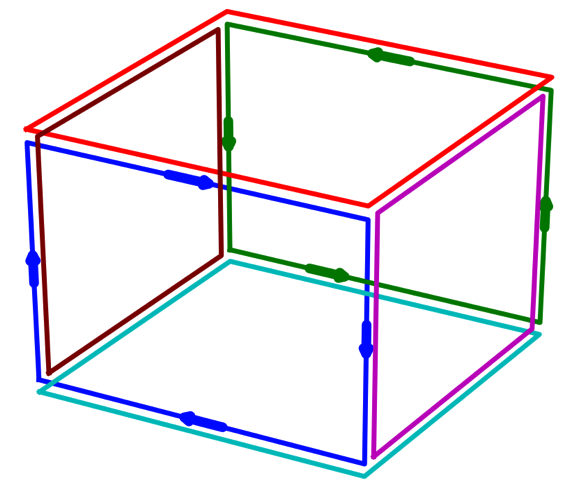
\includegraphics[scale=.28]{Images/c1_4}
        \caption{Current Direction in $C_x^{\pm}$}
        \label{fig:c1}
    \end{subfigure}%
    \begin{subfigure}{.5\linewidth}
        \centering
        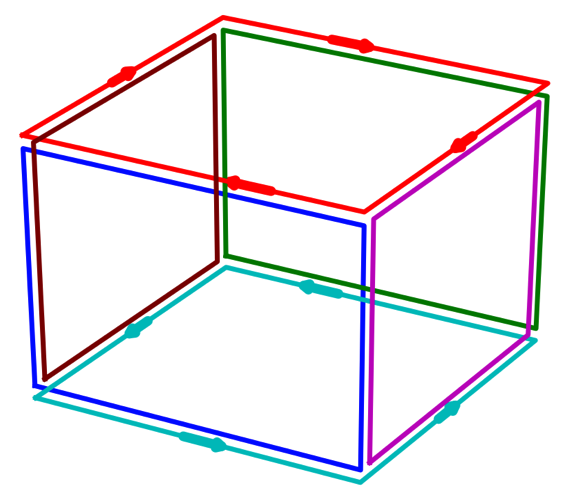
\includegraphics[scale=.28]{Images/c3_4}
        \caption{Current Direction in $C_y^{\pm}$}
        \label{fig:c3}
    \end{subfigure}\\[1ex]
    \begin{subfigure}{\linewidth}
        \centering
        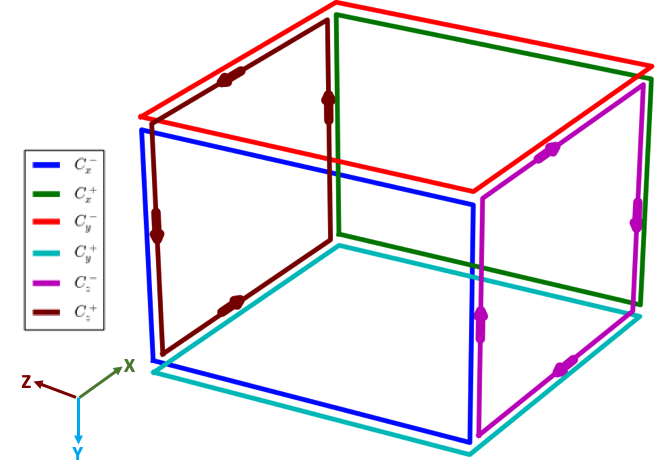
\includegraphics[scale=.33]{Images/c5_4}
        \caption{Current Direction in $C_z^{\pm}$}
        \label{fig:c5}
    \end{subfigure}

\caption[Singular currents corresponding to the singular value $\Sigma_{66}=0$]{Singular currents corresponding to the singular value $\Sigma_{66}=0$.  The currents are equal in magnitude but opposed in direction for each of (a) $C_x^{\pm}$, (b) $C_y^{\pm}$ and (c) $C_z^{\pm}$. When added, the net current (and hence field) is always zero, thus explaining the singular value of zero.}
    \label{fig:cDir}
\end{figure}

We can imagine the elements of the singular vector as describing
eigen-currents.  In row 6, this would describe a set of currents like
those depicted in Fig.~\ref{fig:cDir}.  In this case, if the coils all
overlap perfectly, as they do in this simulation, such a mode has a
net current of zero.  Hence, no matter what the total current applied
to this mode, it will never generate a magnetic field.  Hence the
singular value is always zero.

%\textcolor{red}{The higher frequency information is typically represented by the singular vectors corresponding to the smaller singular values. That is, with increase of n values the left and right singular vectors tend to have more sign changes. The consequence is that the SVD provides us with basis right singular vectors for an expansion where each basis vector represents a certain “frequency,” approximated by the number of times the entries in the vector change signs.}

%It can be as explained by Fig.~\ref{fig:cDir} where one of the coil current mode was shown for all six coils. The total current contribution is found to be zero due to current contributions from $C_x^{\pm}$ in Fig.~\ref{fig:cDir}\textcolor{blue}{(a)}, $C_y^{\pm}$ in Fig.~\ref{fig:cDir}\textcolor{blue}{(b)} and $C_z^{\pm}$ in Fig.~\ref{fig:cDir}\textcolor{blue}{(c)}.


On further inspection, the currents depicted in each of panels (a),
(b), and (c) of Fig.~\ref{fig:cDir} correspond to magnetic field
gradients $\partial B_x/\partial x$, $\partial B_y/\partial y$, and
$\partial B_z/\partial z$, respectively.  These gradients are not
independent of one another because, according to Maxwell's equations:
\begin{equation}
\frac{\partial B_x}{\partial x}+\frac{\partial B_y}{\partial y}+\frac{\partial B_z}{\partial z}=\vec{\nabla}\cdot\vec{B}=0.\label{eq:divb0}
\end{equation}
The problem of the singular value of zero can also be considered in
this differential form.  Consider coils which have been designed which
generate gradients $\partial B_x/\partial x$, $\partial B_y/\partial
y$, and $\partial B_z/\partial z$ near the origin of coordinates.  An
example of such a coil system would be three orthogonal anti-Helmholtz
coils.  If the first two coils are energized to produce uniform
gradients $\partial B_x/\partial x$, $\partial B_y/\partial y$, then
according to Eq.~(\ref{eq:divb0}) they necessarily also generate a
gradient in the $z$ direction
\begin{equation}
\frac{\partial B_z}{\partial z}=-\frac{\partial B_x}{\partial x}-\frac{\partial B_y}{\partial y}.\label{eq:dbzdz}
\end{equation}
The third coil, which generates $\partial B_z/\partial z$ is
therefore unnecessary.  Or conversely, if the third coil is included
in a three-dimensional feedback system, it is possible that the
control system will generate a current in the third coil which
mistakenly counteracts the effect of the other two coils.  This is
essentially what is happening in the case of the bad singular mode
described by Fig.~\ref{fig:cDir}. A general parametrization of the magnetic field in terms of spherical harmonics is proposed by Ref.~\cite{field_abel} and Ref.~\cite{field_jeff} has showed higher order multi-pole corrections to the false EDM of $\mathrm{^{199}Hg}$ spherical traps.

Eq.~(\ref{eq:dbzdz}) suggests one method to prevent the problematic
coil mode from ever being excited: remove the coil which generates
$\partial B_z/\partial z$. This was implemented in the Python
code by requiring that the currents in the $C_z^+$ and $C_z^-$ always
be in the same direction and have the same value, {\it i.e.}~like the
currents in a Helmholtz coil.  This means that there are only five
independently controlled currents, which we denote $C_x^+$, $C_x^-$,
$C_y^+$, $C_y^-$, and $C_z^\pm$.  More about the coils that generate spherical harmonics are discussed in Section~\ref{sec:spherical}.

% \textcolor{red}{Need to add a note here about spherical harmonics. Need to add some note about Rawlik's patch coil system.  Or this could/should go in future work with a forward reference here.}

% \textcolor{red}{Where to add Refs.~\cite{field_abel,field_jeff} ?}
%To break the mode, two out of
%the six coils have been wired together so that they can act as one
%resulting total compensation coils be five.
%It was found that due to this, the condition number is decreased drastically to 2.


% For the prototype, two different configuration of compensation coils have been exploited. In the first case, all the six coils have been used in the six faces surrounding the compensation area and for the later one, two coils have been wired together so that they can act as one making total five instead of six coils. The main reason for using the second configuration is the condition number of $\bm{M}$. It was found to be $\sim$4.7 for the second one as compared to $\sim$51 in the first.


%\textcolor{red}{Is Fig.~\ref{fig:matrix_patch_5c} required ????}

\fig{Images/matrix_patch_5c}{width =0.9\textwidth}{
Color map of $M_{sc}$ elements for 24 fluxgate axes and 5 coils. Coil
dimensions and fluxgate positions are the same as for
Fig.~\ref{fig:matrix_patch_6c}.\label{fig:matrix_patch_5c}}{Matrix for
5 coils.}

The simulated matrix $\bm{M}$ for this configuration is shown in
Fig.~\ref{fig:matrix_patch_5c}.  Naively, it is not considerably
different in terms of the corresponding matrix for six coils, which was
displayed in Fig.~\ref{fig:matrix_patch_6c}.  However, upon performing
the singular value decomposition, the differences become evident.



\fig{Images/Diag_patch_5c}{width =0.9\textwidth}{
Color map of diagonal matrix $\bm{\Sigma}$ found by SVD of simulated
$\bm{M}$ for 24 fluxgate axes and 5
coils. \label{fig:diag_patch_5c}}{Diagonal Matrix for 5 coils.}

Figure~\ref{fig:diag_patch_5c} displays the $\bm{\Sigma}$ matrix
resulting from singular value decomposition.  This results in five
singular values, one for each coil mode.  Most importantly, the
singular value which was zero has been removed from the matrix.  The
remaining singular values are now also all of similar order of
magnitude.  The condition number of the matrix is 2.01, which is a
considerable improvement compared to the infinite condition number of
the six-coil system.

\fig{Images/Right_patch_5c}{width=0.9\textwidth}{Color map of orthogonal matrix $\bm{V^T}$ found by SVD of $\bm{M}$ 24 fluxgate axes and 5 coils. \label{fig:right_patch_5c}}{Orthogonal matrix $\bm{V^T}$ for 5 coils.}

The matrix of right singular vectors $\bm{V^T}$ is displayed in
Fig.~\ref{fig:right_patch_5c}.  The uniform field modes are clearly
visible in rows 1, 3, and 4, corresponding to Helmholtz-like singular
current modes.  Two gradient modes also appear in rows 2 and 5, which
are different combinations of the anti-Helmholtz-like gradients in
each of the $x$ and $y$ directions.


\begin{table} [htb!]
    \centering
    \begin{tabular} { |c|c|c|c|c|c|} 
        \hline
        Coils & \makecell{Matrix \\Condition Number} &\makecell{Inverse Matrix \\ Condition Number} & \makecell{Regularization \\Parameter $r$}\\
        \hline\hline
        \makecell{$C_x^-$, $C_x^+$, $C_y^-$,\\ $C_y^+$, $C_z^-$ and $C_z^+$ } & 26.37 (25.96) & 1.71 (1.61) & 3.04 (2.96) \\ 
        \hline
        \makecell{$C_x^{\pm}$, $C_y^-$, $C_y^+$,\\ $C_z^-$ and $C_z^+$ } & 2.26 (2.05) & 1.08 (1.06) & 3.60 (3.57) \\         
        \hline
        \makecell{$C_x^-$, $C_x^+$, $C_y^\pm$,\\ $C_z^-$ and $C_z^+$ } & 2.27 (2.04) & 1.09 (1.06) & 3.62 (3.54) \\
        \hline
        \makecell{$C_x^-$, $C_x^+$, $C_y^-$,\\ $C_y^+$ and $C_z^\pm$ } & 2.41 (2.09) & 1.10 (1.07) & 3.56 (3.50) \\
        \hline

    \end{tabular}
    % \vspace{4mm}
    \caption[Properties for different coil configurations]{Matrix properties for different 6- and 5-coil configurations for fluxgate sensors at 1, 3, 6 and 8. The values inside the parentheses indicate the calculation done with shield present.}\label{table:mcond_coil}
\end{table}


This solution was then implemented into the active magnetic compensation
system.  Rather than physically wire two coils together, a software solution was used where the currents in one pair of opposing coils
were required to be equal and run in the same direction.

The results of matrix measurement followed by singular value
decomposition are shown in Table~\ref{table:mcond_coil}.  Since $4\times 3$ fluxgate axes could be instrumented, only such matrices
were considered.  The measurements shown inside and outside the parentheses were done with and without the magnetic shield within the coil cube. It is seen that they are similar as expected from the discussion in Section~\ref{sec:shield_impact}.

Table~\ref{table:mcond_coil} shows that the condition number of the
matrix is reduced by more than a factor of ten when comparing the
six-coil solution to the five-coil solution.  Configurations where
opposing coils in the $x$, $y$, and $z$ directions are alternately
selected for the Helmholtz-like current configuration in the five-coil
solution.  Table~\ref{table:mcond_coil} shows that any of these
configurations gave essentially the same results for the condition
number.

Clearly, in the six-coil case, it is an absolute necessity to
regularize the matrix.  As discussed earlier, this may be done by
adjusting the regularization parameter to minimize the condition
number of the Tikhonov regularized pseudoinverse. Tikhonov regularization was also studied for the five-coil case, to see if it had
any impact on the PI feedback system.  Results of the Tikhonov
regularization process are also displayed in
Table~\ref{table:mcond_coil}.

% \fig{Images/coil_reg}{width = \textwidth,height=12cm}{Currents (left vertical axis) in all six coil sides ($C_x^\pm$, $C_y^\pm$ and $C_z^\pm$) with drift $\Delta B$ (right vertical axis) at 12 sensor positions with fluxgate positions 1, 3, 6 and 8 for $k_c^p$=0.0, $k_c^i$=1.0 (see Eq.~(\ref{eq:I})). The $r$=2.9 in (a) and $r$=3.39 in (b). For position of coils and fluxgates see Fig.~\ref{fig:coil}. All grey color curves in $\Delta B$ graph denote the drift in signal that would have been without the compensation while all other color curves denote the actual drift in signal at all 12 sensor positions found by Eq.~(\ref{eq:del_B}). Vertical dashed lines indicate the time of the perturbation coil being turned on and off. The current supplied on perturbation coil was 10  mA. The resolution index 1 (see Table~\ref{table:t7freq}) with 50 no of averages per measurement used. The loop sampling frequency was found to be $\sim$6.5 Hz.\label{fig:coil_reg}}{Coil currents with drift $\Delta B$ for different coil configuration in regularized $\bm{M^{-1}}$}
\fig{Images/coil_reg4}{width=\textwidth,height=12cm}{(a) 6-coil feedback algorithm compared with (b) 5-coil feedback algorithm, where the only change is that the currents $C_x^+$ and $C_x^-$ are required to be a common current $C_x^\pm$.  Both pseudoinverses have been regularized using the method described Section~\ref{sec:new_study_r}.  Coil currents are shown in the left panels while magnetic field changes are shown  in the right panels.
In both (a) and (b), the feedback parameters are $k_c^p=0.0$ and
$k_c^i=1.0$.\label{fig:coil_reg}}{Coil currents with field change
$\Delta B$ for different coil configurations in regularized
$\bm{M^{-1}}$}

Figure~\ref{fig:coil_reg} shows experimental data which demonstrate
the success of the five-coil method compared to the six-coil method.
In this case, we have compared the matrices with our regularization
method, determining the best value of $r$ based on its ability to
minimize the condition number of the resultant pseudo-inverse (see
Section~\ref{sec:cond}).
Figs.~\ref{fig:coil_reg}\textcolor{blue}{(a)}
and \textcolor{blue}{(b)} correspond to the settings described in the
first two rows of Table~\ref{table:mcond_coil}.

The main success is that in the five-coil algorithm, the currents
settle rapidly after the excitation coil has been switched on, and
return rapidly to their initial values when switched off.  This can be
contrasted with the six-coil algorithm where the current drifting
problem is quite evident: the coil currents take more than ten seconds
to settle.

Another clear success is that in the five-coil case, the coil $C_z^+$,
which is {\it closest} to the perturbation coil, is the one that has
the most current driven by the feedback algorithm.  Certainly this
would be the expected result.  In the six-coil case,
Fig.~\ref{fig:coil_reg}\textcolor{blue}{(a)} demonstrates that the initial coil
responses are quite similar to the five-coil method (within the first
$<1$~s), but then the current drifting problem sets in, and the
currents grow in coils where one would expect them to be small.  The
growth of the problematic mode with singular value zero is also quite
evident in the six-coil case: the currents in opposite coils have
opposite changes relative to the initial current and are roughly equal
in magnitude.  This is the mode that in the ideal simulation does not
generate any magnetic field.  Because of the smallness of the effect
of this mode, the six-coil algorithm tends to set the current to a
somewhat arbitrary value.

In both the five-coil and six-coil cases, the overall results for the
reduction in the magnetic field at the control sensor positions are
quite similar.  Some small, longer term drifts in the six-coil case
can be seen.  We expect that this happens because the field generated
by the problematic mode is small but non-zero, because the coils do
not exactly overlap as they do in the ideal simulation.  There is some
evidence that there is additional higher frequency noise in the
six-coil case, which could be coming from the considerably larger and
less stable currents generated by the problematic mode.

So, while the two algorithms give similar results for the generated
magnetic fields, clearly the five-coil algorithm is more desirable
because smaller coil currents with smaller random fluctuations are
generated.  The five-coil system is clearly responding to a field in
the $z$-direction that is located near the $C_z^+$ coil.

% \fig{Images/coil_pseudo}{width = \textwidth,height=12cm}{Currents (left vertical axis) in all six coil sides ($C_x^\pm$, $C_y^\pm$ and $C_z^\pm$) with drift $\Delta B$ (right vertical axis) at 12 sensor positions with fluxgate positions 1, 3, 6 and 8 for $k_c^p$=0.0, $k_c^i$=1.0 (see Eq.~(\ref{eq:I})). Pseudoinverse was used in both case. For position of coils and fluxgates see Fig.~\ref{fig:coil}. All grey color curves in $\Delta B$ graph denote the drift in signal that would have been without the compensation while all other color curves denote the actual drift in signal at all 12 sensor positions found by Eq.~(\ref{eq:del_B}). Vertical dashed lines indicate the time of the perturbation coil being turned on and off. The current supplied on perturbation coil was 10  mA. The resolution index 1 (see Table~\ref{table:t7freq}) with 50 no of averages per measurement used. The loop sampling frequency was found to be $\sim$6.5 Hz.\label{fig:coil_pseudo}}{Coil currents with drift $\Delta B$ for different coil configuration in non-regularized $\bm{M^{-1}}$}

\fig{Images/coil_pseudo3}{width =\textwidth,height=12cm}{(a) 6-coil feedback algorithm compared with (b) 5-coil feedback algorithm, where the only change is that the currents $C_x^+$ and $C_x^-$ are required to be a common current $C_x^\pm$.  No regularization of the pseudoinverse has been done in either case.  All other parameters are the same as for Fig.~\ref{fig:coil_reg}.\label{fig:coil_pseudo}}{Coil currents with field change
$\Delta B$ for different coil configurations with non-regularized
$\bm{M^{-1}}$.}

The five-coil algorithm can even be operated without the need for
Tikhonov regularization of the pseudo-inverse.
Figure~\ref{fig:coil_pseudo} compares the six-coil and five-coil
algorithms when no regularization is performed.  The five-coil case
performs well, perhaps even better than the results displayed in
Fig.~\ref{fig:coil_reg}\textcolor{blue}{(b)} because the field
fluctuations are smaller.  This might also indicate that the PI
feedback parameters are not fully optimal, since more overshoot is
also evident in Fig.~\ref{fig:coil_pseudo}\textcolor{blue}{(b)} when
compared to Fig.~\ref{fig:coil_reg}\textcolor{blue}{(b)}.  For this
study, the feedback parameters were held constant, and in
Section~\ref{sec:new_study_r}, a relationship
between these parameters was shown.  Additional optimization is possible and
could affect this conclusion.

In general, we expect that the non-regularized solution is superior.
Tikhonov regularization introduces additional constraints in order
attempt to keep a poorly conditioned feedback system from oscillating.
It is a superior principle to design the system to be well-conditioned
rather than relying on Tikhonov regularization to solve the problem of
ill-conditioning.  This is also one of the general conclusions of
Ref.~\cite{rawlik}.

In Figs.~\ref{fig:matrix_patch_6c} and \ref{fig:matrix_patch_5c}, the ideal simulation results of the matrix $\bm{M}$ is shown.  The matrix $\bm{M}$ measured
experimentally is similar in its structure to these simulation
results.

\fig{Images/diag_comb}{width=\textwidth,height=5.5cm}{Color map of diagonal matrix $\bm{\Sigma}$ found by SVD of experimentally measured
$\bm{M}$ for the available 12 fluxgate axes and for (a) 5 coils,
where the $C_x^\pm$ coils are required to carry the same current,
and (b) 6 coils which, are permitted to carry any
current.\label{fig:diag_comb}}{Experimental results for the
$\bm{\Sigma}$ matrix.}

It is interesting to compare the results for the diagonal matrix
$\bm{\Sigma}$ in simulation and experiment.  The experimental results
for $\bm{\Sigma}$ are presented in Fig.~\ref{fig:diag_comb}, for both
the five-coil and six-coil case.  These can be compared with the
simulated results which were presented in
Figs.~\ref{fig:diag_patch_5c} and \ref{fig:diag_patch_6c}.  It can be
seen that, despite having only 12 fluxgate axes available
experimentally, the $\bm{\Sigma}$ matrices compare favorably with the
simulated counterparts.  In general the matrix elements are smaller
experimentally, but this is simply because the fluxgates were located
about 8-10~cm inside the corner positions of the coil cube, whereas in
the previously presented simulations, they were only 2~cm inside and
hence were closer to the coils.

The main similarity is in the trends of the singular values and in the
condition number of the matrix.  In the five-coil case, the singular
values are all the same order of magnitude, and the condition number
is 2.26 (see also Table~\ref{table:mcond_coil}).  In the six-coil
case, the first five singular values are of similar orders of
magnitude, and the sixth is significantly smaller.  In the simulation
(Fig.~\ref{fig:diag_patch_6c}), this singular value was exactly zero.
We expect the difference (zero vs.~non-zero) is due to the currents
not exactly overlapping in the experimental case.

\fig{Images/right_comb}{width = \textwidth,height=5.5cm}{Experimentally determined right singular vectors, represented by the rows of the matrix $\bm{V^T}$ resulting from SVD of the experimentally measured matrix $\bm{M}$.\label{fig:right_comb}}{Experimentally measured right singular vectors.}

Similarities can also be seen in the right singular vectors, described
by the rows of the $\bm{V^T}$ matrix.  The experimental results for
the right singular vectors are presented in Fig.~\ref{fig:right_comb}
and can be compared with the simulation results which were presented
in Figs.~\ref{fig:right_patch_6c} and \ref{fig:right_patch_5c}.  In
Fig.~\ref{fig:right_comb}\textcolor{blue}{(b)}, the problematic mode
corresponding to the smallest singular value can indeed be seen to
result from opposing currents of nearly equal magnitude being
generated in each of the six coils.  In the five-coil experimental
results shown in Fig.~\ref{fig:right_comb}\textcolor{blue}{(a)}, a similar pattern of singular vectors
can be seen as for the simulated version presented in
Fig.~\ref{fig:right_patch_5c}.  Row 1 corresponds to the uniform field
in the $x$-direction.  Rows 2 and 5 appear to correspond to admixtures
of gradients in the $y$ and $z$ directions.  Row 3, having two red
values in $C_y^+$ and $C_y^-$ most closely corresponds to a uniform
field in the $y$-direction, whereas row 4 corresponds most closely to
the uniform field in the $z$-direction.  There is some admixture of
the identities of the singular vectors which are likely due to some
experimental geometrical imperfections.



\fig{Images/5c_z}{width=\textwidth}{Five-coil feedback algorithm, where the currents $C_z^+$ and $C_z^-$ are required to be a common current $C_z^\pm$.  Tikhonov regularization of the pseudoinverse has been done, although the results would be very similar even without this.  All other parameters are the same as for Fig.~\ref{fig:coil_reg}.\label{fig:5c_z}}{Five-coil feedback results for common $C_z^\pm$ configuration.}

In Fig.~\ref{fig:coil_reg}\textcolor{blue}{(b)}, it was shown that the dominant current
response to the excitation coil was in the $C_z^+$ coil.  The reason
for this is that the $C_z^+$ coil is located at the closest position
and in the correct direction to cancel the field coming from the
excitation coil.  For that study, the $C_x^\pm$ coils were required to
have a common current.  We were interested to study the effect on the
five-coil feedback algorithm if common current was required in the
$C_z^\pm$ coils instead.

The results of this alternate choice are shown in Fig.~\ref{fig:5c_z}.
Turning on the excitation coil indeed causes the common $C_z^\pm$
current to become more positive with have the change of the previous
result for $C_z^+$ in Fig.~\ref{fig:coil_reg}\textcolor{blue}{(b)}.  The system now must
generate a large gradient in the $z$-direction.  This is achieved by
generating roughly equal gradients $\partial B_x/\partial x$ and
$\partial B_y/\partial y$ using the other four coils which then
generates the required gradient $\partial B_z/\partial z$ according to
Eq.~(\ref{eq:dbzdz}).

We think an interesting point in this case is that, for this particular
positioning of the perturbation coil, it would clearly be desirable
for the system itself to be able to generate different currents in
$C_z^+$ and $C_z^-$ if aiming to have the smallest changes in the
currents.

%\subsection{Extra Data}
%\begin{itemize}
%\item Some data with shield inside.
%\begin{enumerate}
%\item Something like $\bm{\Sigma}$ for the 5- and 6-coil.
%\item An example of the feedback system operating.
%\item Internal sensor perturbations (could appear in next section)
%\item Allan deviations (could appear in next section also) ... possibly with different or no excitation coil.  (slow ramp?  step function? ...)
%\end{enumerate}
%\end{itemize}


The tests were also redone with the magnetic shield inside the coil cube.
Not surprisingly, the conclusions were the same.

%\fig{Images/matrix_comb_shield}{width = \textwidth}{.. \label{fig:matrix_comb_shield}}{S}

\fig{Images/diag_comb_shield}{width=\textwidth,height=5.5cm}{Color map of diagonal matrix
$\bm{\Sigma}$ with the magnetic shield in place found by SVD of
experimentally measured $\bm{M}$ for the available 12 fluxgate axes
and for (a) 5 coils, where the $C_x^\pm$ coils are required to
carry the same current, and (b) 6 coils which, are permitted to carry
any current.\label{fig:diag_comb_shield}}{Experimental results for the
$\bm{\Sigma}$ matrix with the magnetic shield in place.}

Figure~\ref{fig:diag_comb_shield} shows the results for the
$\bm{\Sigma}$ matrix when the magnetic shield is in place.  The
general trends in the singular values are very similar as in the case
without the magnetic shield.  As reported in
Table~\ref{table:mcond_coil}, the condition number in the five-coil
case is 2.05 and in the six-coil case it is 25.96.

%\fig{Images/right_comb_shield}{width = \textwidth}{Experimentally determined right singular vectors, represented by the rows of the matrix $\bm{V^T}$ resulting from SVD of the experimentally measured matrix $\bm{M}$.\label{fig:right_comb_shield}}{Experimentally measured right singular vectors.}

The right singular vectors corresponding to the coil modes also show
similar trends.  For the six-coil case, the same problematic mode is
present.  For the five-coil case, the same general mode structure is
apparent, consisting of three uniform field modes and two gradient
modes in the same pattern.

%\fig{Images/6c_reg_shield}{width = \textwidth}{6c reg shield. \label{fig:6c_reg_shield}}{S}

%\fig{Images/6c_pseudo_shield}{width = \textwidth}{6c pseudo shield. \label{fig:6c_pseudo_shield}}{S}
 
%\fig{Images/5c_pseudo_shield_x}{width = \textwidth}{$C_x^\pm$, $C_y^-$, $C_y^+$, $C_z^-$ and $C_z^+$ . \label{fig:5c_pseudo_shield_x}}{S}

\fig{Images/5c_pseudo_shield_y}{width = \textwidth}{Five-coil feedback
algorithm with the magnetic shield placed inside the coil cube.  The
currents $C_y^+$ and $C_y^-$ are required to be a common current
$C_y^\pm$.  All other parameters are the same as for
Fig.~\ref{fig:coil_reg}.\label{fig:5c_pseudo_shield_y}}{Five-coil
feedback results with the magnetic shield inside the coil cube.}

The improvement in the general feedback system operation for the
five-coil feedback algorithm is also very clear when the magnetic
shield is within the coil cube.  Results of the usual test with the
excitation coil are shown in Fig.~\ref{fig:5c_pseudo_shield_y}, where
the non-regularized pseudo-inverse has been used.  For
Fig.~\ref{fig:5c_pseudo_shield_y}, the $C_y^+$ and $C_y^-$ coils have
been required to carry a common current $C_y^\pm$ while the other five
coils may be adjusted freely.  Even with the magnetic shield present,
the results are very similar to Fig.~\ref{fig:coil_pseudo}\textcolor{blue}{(b)} where no
shield was present. The results were also compared with redid in PI simulations and a similar behaviour was observed as expected.


%\fig{Images/5c_pseudo_shield_z}{width = \textwidth}{$C_x^-$, $C_x^+$, $C_y^-$, $C_y^+$ and $C_z^\pm$. \label{fig:5c_pseudo_shield_z}}{S}

%\fig{Images/i_rm_comb}{width = \textwidth}{.. \label{fig:i_r_comb}}{S}
%\fig{Images/matrix_comb}{width = \textwidth}{.. \label{fig:matrix_comb}}{S}

%\fig{Images/5c_x}{width = \textwidth}{$C_x^{\pm}$, $C_y^-$, $C_y^+$, $C_z^-$ and $C_z^+$. \label{fig:5c_x}}{S}

%\fig{Images/5c_x_all}{width = \textwidth}{$C_x^{\pm}$, $C_y^-$, $C_y^+$, $C_z^-$ and $C_z^+$. \label{fig:5c_x_all}}{S}
 
%\fig{Images/5c_y}{width = \textwidth}{$C_x^-$, $C_x^+$, $C_y^\pm$, $C_z^-$ and $C_z^+$ . \label{fig:5c_y}}{S}

%\fig{Images/5c_y_all}{width = \textwidth}{$C_x^-$, $C_x^+$, $C_y^\pm$, $C_z^-$ and $C_z^+$. \label{fig:5c_y_all}}{S}
%\fig{Images/5c_z_all}{width = \textwidth}{$C_x^-$, $C_x^+$, $C_y^-$, $C_y^+$ and $C_z^\pm$. \label{fig:5c_z_all}}{S}



%\begin{table} [htb!]
%    \centering \begin{tabular} { |c|c|c|c|c|c|} \hline Coils
%    & \makecell{Matrix \\Condition Number} &\makecell{Inverse
%    Matrix \\ Condition Number}
%    & \makecell{Regularization \\Parameter,
%    $r$}\\ \hline\hline \makecell{$C_x^-$, $C_x^+$, $C_y^-$,\\
%    $C_y^+$, $C_z^-$ and $C_z^+$ } & 26.37 & 1.71 &
%    3.04 \\ \hline \makecell{$C_x^{\pm}$, $C_y^-$, $C_y^+$,\\ $C_z^-$
%    and $C_z^+$ } & 2.26 & 1.08 & 3.6 \\ \hline \makecell{$C_x^-$,
%    $C_x^+$, $C_y^\pm$,\\ $C_z^-$ and $C_z^+$ } & 2.27 & 1.09 &
%    3.62 \\ \hline \makecell{$C_x^-$, $C_x^+$, $C_y^-$,\\ $C_y^+$ and
%    $C_z^\pm$ } & 2.41 & 1.10 & 3.56 \\ \hline \makecell{$C_x^-$,
%    $C_x^+$+$C_y^-$,\\ $C_y^+$, $C_z^-$ and $C_z^+$ } & 2.97 & 1.14 &
%    3.6 \\ \hline \makecell{$C_x^-$, $C_x^+$,$C_y^-$,\\
%    $C_y^+$+$C_z^-$ and $C_z^+$ } & 2.8 & 1.14 &
%    3.62 \\ \hline \makecell{$C_x^-$+$C_y^-$, $C_x^+$,\\
%    $C_y^+$,$C_z^-$ and $C_z^+$ } & 25 & 1.69 &
%    3.06 \\ \hline \makecell{$C_x^-$, $C_x^+$+$C_y^+$,\\ $C_y^-$,
%    $C_z^-$ and $C_z^+$ } & 25 & 1.70 &
%    3.05 \\ \hline \makecell{$C_x^-$, $C_x^+$, $C_y^+$,\\
%    $C_y^-$+$C_z^-$ and $C_z^+$ } & 26.14 & 1.65 &
%    3.06 \\ \hline \makecell{$C_x^-$+$C_x^+$, $C_y^-$+
%    $C_y^+$,\\$C_z^-$ and $C_z^+$ } & 440.57 & 1.79 &
%    2.54 \\ \hline \makecell{$C_x^-$+$C_x^+$, $C_y^-$+ $C_y^+$,\\ and
%    $C_z^-$+$C_z^+$ } & 1.27 & 1.0 & 3.73 \\ \hline
%
%    \end{tabular}
%    % \vspace{4mm}
%    \caption[Properties for different coil configurations]{Matrix properties for different 6- and 5-coil configurations for fluxgate sensors at 1, 3, 6 and 8.}\label{table:mcond_coi2}
%\end{table}








%\subsection{Extra Data} % (copied from previous Section)



%\subsection{Experimental Current Error and Remaining Fluctuation... maybe change this into a discussion on better ideas beyond regularization, such as spherical harmonics, patch coils, and how this can lead to a properly regularized system that is more flexible.}

%\begin{itemize}
%\item Basic message of Fig. 5.4 is that experiment and simulation kind of agree.
%% \item In simulation a set of twelve $B_s^\text{rand}$ has been generated by normal distribution around zero with standard deviation being 1.5 nT.
%% % \item In experiment  set of twelve $B_s^\text{rand}$ has been generated by magnetic field signals from fluxgate positions at 1, 2 and 7 using Eq.~(\ref{eq:del_B}). For position of the fluxgates please see Fig.~\ref{fig:coil}.
%% \item $r$ has been varied from 0 to 6 in an increment of 0.29 and for each $r%$, PI control algorithm has been implemented for n measurements and for every measurements, signals from fluxgates at positions 1,2 and 7 are stored as $B_{\text{meas}}$ and uncompensated B field has been stored as $B_{\text{uncomp}}$ using  $B_{\text{meas}}-\bm{M}(I_c^n-I_c^0)$ where $I_c^n$ can be found using Eq.~(\ref{eq:I}). From those stored values,  Eq.~(\ref{eq:B_coils-sim}) has been found by $B_{\text{meas}}^{\text{max}}(r)-B_{\text{meas}}^{\text{min}}(r)$ and $B_s^\text{rand}$ has been found by $B_{\text{uncomp}}^{\text{max}}(r)-B_{\text{uncomp}}^{\text{min}}(r)$ and $\Delta I_c^{\text{exp}}(r)$ has been found using same as Eq.(\ref{eq:del_Is}). 
%\end{itemize}

%\fig{Images/mont_exp}{width = \textwidth}{The effect of $r$ on (a) current error  and (b) remaining field fluctuations in experimental setup for $k_c^p=1.0$ for fluxgate signals from 1, 2 and 7. Here, 100 mA current has been supplied in the perturbation coil. For position of the fluxgates  and coil see Fig.~\ref{fig:coil}.\label{fig:mont_comp}}{The effect of $r$ for experimental setup.}

%The effect of $r$ on the current error and remaining field
%fluctuations in experimental setup for fluxgate signals from 1, 2 and
%7 are shown in Fig.~\ref{fig:mont_comp}. For position of the sensors
%please see Fig.~\ref{fig:coil}. For data measurement, for certain
%loops, PI control algorithm with $k_c^p=$1.0 and $k_c^i=$0.0 has been
%implemented for $r$ ranges from 0 to 6 in an increment of 0.29. For
%every measurements, signals from fluxgates at positions 1,2 and 7 are
%stored as $B_{\text{meas}}$ and uncompensated B field has been stored
%as $B_{\text{uncomp}}$ which is predicted by Eq.~\ref{eq:Buncomp}. The
%difference between maximum value of $B_{\text{uncomp}}$ and
%$B_{\text{uncomp}}$ will give the field fluctuation due to 100 mA
%supplied in rhe perturbation coil. Moreover, the difference between
%maximum value of $B_{\text{meas}}$ and $B_{\text{meas}}$ will give the
%amount of compensation of the field which when equal to field
%fluctuation indicates no compensation. The ratio of rms value of this
%to the field fluctuation will generate the remaining fluctuation $F$
%which is shown for different $r$ in
%Fig.~\ref{fig:mont_comp}\textcolor{blue}{(b)}. It is seen that for a
%particular filed perturbation, the remaining fluctuation is
%$\approx$0.45 which indicates that the maximum correction is
%$\mathbf{(1-0.45)\times100\%=55\%}$. Moreover, $\Delta
%I_c^{\text{exp}}(r)$ has been found using Eq.(\ref{eq:del_Is}) and the
%rms has been determined which is shown in
%Fig.~\ref{fig:mont_comp}\textcolor{blue}{(a)}. It is seen that around
%100 mA rms of current array is required to compensate the perturbation
%which eventually vanishes with $r$ increment as expected.
% We have studied the coil current response and magnetic fluctuation reduction in

% In Section~\ref{sec:inv}, we have already talked about how the regularization parameter $r$ came into effect. Then, in Section~\ref{sec:mont}, regularization by random magnetic distribution method has been described which has been taken from Ref.~\cite{bea} where a suitable value of $r$ has been found which will give the best compromise between the magnetic field fluctuation and coil current fluctuation. We have generated a fluctuation by our perturbation coil. $r$ has been varied from 0 to 6 in an increment of 0.29 and for each $r$, PI control algorithm has been implemented for n measurements and for every measurements, signals from fluxgates at positions 1,2 and 7 are stored as $B_{\text{meas}}$ and uncompensated B field has been stored as $B_{\text{uncomp}}$ using  $B_{\text{meas}}-\bm{M}(I_c^n-I_c^0)$ where $I_c^n$ can be found using Eq.~(\ref{eq:I}). From those stored values,  Eq.~(\ref{eq:B_coils-sim}) has been found by $B_{\text{meas}}^{\text{max}}(r)-B_{\text{meas}}^{\text{min}}(r)$ and $B_s^\text{rand}$ has been found by $B_{\text{uncomp}}^{\text{max}}(r)-B_{\text{uncomp}}^{\text{min}}(r)$ and $\Delta I_c^{\text{exp}}(r)$ has been found using same as Eq.(\ref{eq:del_Is}). 

% The root mean square (RMS) of $\Delta I_c^{\text{exp}}(r)$ is calculated as
% \begin{equation}\label{eq:delta_Iexp_rms}
%      \Delta I_{\text{RMS}}^{\text{exp}}(r)= \sqrt{\frac{1}{6}\sum_{c=1}^6 (\Delta I_c^{\text{exp}}(r))^2}
% \end{equation}
% The remaining fluctuation is calculated as
% \begin{equation}\label{eq:fluc}
%     F(r)=\frac{\sqrt{\frac{1}{12} \sum_{s=1}^{12} (B_s^{\text{sim}}(r))^2}}{\sqrt{\frac{1}{12} \sum_{s=1}^{12} (B_s^{\text{rand}}(r))^2}}
% \end{equation}
% The field without compensation is predicted by 
% \begin{equation}
    
% \end{equation}
% In this Section, we have found Eq.~(\ref{eq:delta_Isim_rms}) and Eq.~(\ref{eq:fluc}) in experimental setup.
% $B_s^{\text{rand}}$ will be replaced by
% The fluctuation caused by perturbation coil is
% \begin{equation}\label{eq:B_coils-exp}
%     B_s^{\text{fluc}}(r) =B_{\text{uncomp}}^{\text{max}}(r)-B_{\text{uncomp}}^{\text{min}}(r)
% \end{equation}
% To compensate the fluctuation
% \begin{equation}\label{eq:B_coils-exp}
%     B_s^{\text{exp}}(r) =B_{\text{meas}}^{\text{max}}(r)-B_{\text{meas}}^{\text{min}}(r)
% \end{equation}


% \begin{equation}\label{eq:fluc_exp}
%     F(r)=\frac{\sqrt{\sum_s \frac{1}{s}(B_{\text{meas}}^{\text{max}}(r)-B_{\text{meas}}^{\text{min}}(r))^2}}{\sqrt{\sum_s \frac{1}{s}(B_{\text{uncomp}}^{\text{max}}(r)-B_{\text{uncomp}}^{\text{min}}(r))^2}}
% \end{equation}

% In Section~\ref{sec:mont}, 30 different sets of random magnetic field ($B_s^{\text{rand}}$) values have been chosen with center of distribution being 0 and standard deviation 5 nT for 12 different fluxgate sensor positions whose labels are given in the horizontal axis of Fig.~\ref{fig:m} and the positions are specified in Fig.~\ref{fig:coil}. Here, we have chosen one out of the 30 different sets of $B_s^{\text{rand}}$ and go through the steps as in Section~\ref{sec:mont} to generate similar figures like in Fig.~\ref{fig:Isim}, Fig.~\ref{fig:fluc-sim} and Fig.~\ref{fig:I-fluc}. For the experimental setup, we have done the similar steps to generate those figures except instead of generating $B_s^{\text{rand}}$ randomly, we have applied current in the perturbation coil to generate the required drift ( see Eq.~(\ref{eq:del_B}) ) which will be treated as $B_s^{\text{rand}}$. The results of the simulation as well as experiment are given in Fig.~\ref{fig:mont_comp}, where Fig.~\ref{fig:mont_comp}\textcolor{blue}{(a)}, Fig.~\ref{fig:mont_comp}\textcolor{blue}{(b)} and Fig.~\ref{fig:mont_comp}\textcolor{blue}{(c)} are the results found from simulation and Fig.~\ref{fig:mont_comp}\textcolor{blue}{(d)}, Fig.~\ref{fig:mont_comp}\textcolor{blue}{(e)} and Fig.~\ref{fig:mont_comp}\textcolor{blue}{(f)} are the results found from experiment. They are described in detail in Fig.~\ref{fig:Isim}, Fig.~\ref{fig:fluc-sim} and Fig.~\ref{fig:I-fluc}. It is seen that the experimental counterpart of each of the simulation that is Fig.~\ref{fig:mont_comp}\textcolor{blue}{(a)} of simulation is comparable to Fig.~\ref{fig:mont_comp}\textcolor{blue}{(d)} of experiment. Similarly, Fig.~\ref{fig:mont_comp}\textcolor{blue}{(b)} of simulation with Fig.~\ref{fig:mont_comp}\textcolor{blue}{(e)} of experiment and Fig.~\ref{fig:mont_comp}\textcolor{blue}{(c)} of simulation with Fig.~\ref{fig:mont_comp}\textcolor{blue}{(f)} of experiment are comparable and they produce similar results. The similar results of the simulation with experiment justifies the the simulation model described in Section~\ref{sec:mont}.

% \fig{Images/mont_comp3}{width = \textwidth,height =10cm}{Simulation result for one set of $B_s^{\text{rand}}$ for the Fig.~\ref{fig:Isim}, Fig.~\ref{fig:fluc-sim} and Fig.~\ref{fig:I-fluc} are shown in (a), (b) and (c) and corresponding experimental results are in (d), (e) and (f). For the description of the figures see the text in Fig.~\ref{fig:Isim}, Fig.~\ref{fig:fluc-sim} and Fig.~\ref{fig:I-fluc}. For position of fluxgate sensors see Fig.~\ref{fig:coil}.\label{fig:mont_comp}}{Short}



% The above results in Fig.~\ref{fig:mont_comp}, where simulation results are similar to experimental one justify the simulation method described in Section~\ref{sec:mont}. The upcoming Section is all about P and I term (see Eq.~(\ref{eq:I}) ) behaviour. 
% \fig{Images/sf6p}{width = \textwidth}{p127, 100mA stimulus,p0.7,r3.5,Simulation result for one set of $B_s^{\text{rand}}$ for the Fig.~\ref{fig:Isim}, Fig.~\ref{fig:fluc-sim} and Fig.~\ref{fig:I-fluc} are shown in (a), (b) and (c) and corresponding experimental results are in (d), (e) and (f). For the description of the figures see the text in Fig.~\ref{fig:Isim}, Fig.~\ref{fig:fluc-sim} and Fig.~\ref{fig:I-fluc}. For position of fluxgate sensors see Fig.~\ref{fig:coil}.\label{fig:adev}}{Short}

\section{Other metrics of feedback system performance}\label{sec:metrics_res}

%\begin{enumerate}
%\item Allan deviations ... possibly with different or no excitation coil.  (slow ramp?  step function? ...)
%\item Internal sensor perturbations (related to previous section).
%\end{enumerate}

In Section~\ref{sec:metrics}, some additional
quantitative measures of the magnetic compensation performance were introduced.  These
metrics had been used in the previous studies of
Refs.~\cite{bea,lins,rawlik}.  The two metrics that will be discussed further in this section are
\begin{itemize}
\item the readings of central internal sensors when the compensation system is used, and
\item the Allan standard deviation, which is used to gauge the effectiveness of corrections over long timescales.
\end{itemize}
The general conclusion of these studies is that they are in
qualitative agreement with the previous works of others.  We also
believe that one of the main limiting factors relates to the need for
more advanced coil design, which is discussed further in
Chapter~\ref{ch:conclusion}.


\subsection{Internal Sensor Perturbations}

Most of the results that was showed so far are related to the magnetic field
measured by 12 fluxgate sensors positioned within the coil cube just
outside the region of interest.  Normally when these data were taken,
we simultaneously acquired data for two additional fluxgate axes placed
centrally within the coil cube.  These sensors were not used in the
feedback algorithm.  The idea was to use these as a way to estimate
average feedback system performance within the region of interest.

\fig{Images/center_6c_reg_sNs}{width = \textwidth}{Central magnetic field in
the $z$ (blue) and $x$ (red) directions.  The 6-coil feedback
algorithm was used.  The left graphs show the case when the magnetic
shield (the outermost layer of the 4-shell system) is present.  The
right graphs show the case when no magnetic shield is present.  A
current of 10 mA was applied to the perturbation coil.
\label{fig:center_6c_reg}}{Central magnetic field in
the $z$ and $x$ directions, 6-coil feedback algorithm.}

Figure~\ref{fig:center_6c_reg} shows the magnetic fluctuation
reduction on the central sensors in $z$, and $x$ axis for the 6-coil
feedback algorithm discussed in the previous Section.  Results are
compared when the outermost magnetic shield of the four-shell magnetic
shielding system is present.  The presence of the magnetic shield
reduces the perturbation of the central field by a factor of 25.
Otherwise the results are quite comparable, showing a similar
fractional reduction of the effect of the perturbation, which is
dominantly in the $z$ direction.  The central field in the $z$
direction is reduced by a factor $\sim 2/3$.

%without shield (right). Aside from the vertical axis, the results are
%similar both with shield and no shield. The magnetic field changes are
%reduced by 0.5 nT in case of with shield with the uncompensated field
%change is 1.25 nT and 15 nT in case without shield with the
%uncompensated field change is 37 nT in $z$ axis. It is also seen that
%there is hardly any changes in $x$ due to perturbation.

%Similar effect can also be seen in case of non-regularized pseudo-inverse of $\bm{M^{-1}}$ in Fig.~\ref{fig:center_6c_pseudo}.


%\fig{Images/center_6c_pseudo_sNs}{width = \textwidth}{6coils, shield, no shield, 10 mA perturbation, $k_c^p=0.0$, $k_c^i=1.0$, non-regularized pseudo-inverse of $\bm{M^{-1}}$.. \label{fig:center_6c_pseudo}}{S}

\fig{Images/center_pseudo_perturb_5c_x}{width = \textwidth}{Central magnetic field in
the $z$ (blue) and $x$ (red) directions.  The 5-coil feedback
algorithm was used, with the currents $C_x^\pm$ being constrained to
be equal.  The outermost layer of the magnetic shielding system was
placed around the sensors and within the coil
cube.\label{fig:center_pseudo_5c_x}}{The 5-coil feedback
algorithm}

The results are virtually identical if the 5-coil feedback algorithm
is used (Fig.~\ref{fig:center_pseudo_5c_x}).  This is not surprising
because generally the magnetic field results were often quite similar
for the 5- and 6-coil algorithms when properly tuned, despite the
currents in the 6-coil algorithm experiencing the current drifting
problem.

%\fig{Images/center_5c_pseudo_s_xz}{width = \textwidth}{5coils, $C_x^\pm$ (left),$C_z^\pm$ (right), shield, 44 mA perturbation, $k_c^p=0.0$, $k_c^i=0.6$, non-regularized pseudo-inverse of $\bm{M^{-1}}$.. \label{fig:center_5c_pseudo_s_xz}}{S}


%I have also studied in case of five coils configuration which also
%give similar results as can be seen by
%Fig.~\ref{fig:center_pseudo_5c_x} and
%Fig.~\ref{fig:center_5c_pseudo_s_xz}.

We also did various other trials varying the feedback system
parameters, and adjusting the current applied to the perturbation
coil, both with and without the magnetic shield present.  In general
the reduction in the central $z$ field was similar.

While it is not a large reduction, the result is relatively consistent
with our results for the general reduction in the field at the external
sensor sites when the feedback system is used to correct the effect of
the perturbation coil (see the previous Section).  In that case also,
the general reduction in the field at the external sensor sites was by a factor of roughly 1/2 to 2/3 on average.  We expect that in
order to provide better overall compensation results, the chief
improvement will be in coil design, which was beyond the scope of this
thesis.

%\fig{Images/5c_pseudo_s_xz}{width = \textwidth}{5coils, $C_x^\pm$ (a),$C_z^\pm$ (b), shield, 44 mA perturbation, $k_c^p=0.0$, $k_c^i=0.6$, non-regularized pseudo-inverse of $\bm{M^{-1}}$.. \label{fig:5c_pseudo_s_xz}}{S}


%The goal of the prototype is to reduce $\sim 200$ nT filed change. Fig.~\ref{fig:5c_pseudo_s_xz} shows the magnetic compensation result due to twelve compensation fluxgate sensors.  It is seen that the prototype is successfully reduce the $\sim 200$ nT filed change.

%\FloatBarrier

\subsection{Allan Deviation Results}\label{sec:adev_res}

The definition of the Allan standard deviation and the ``shielding
factor'' were discussed in Section~\ref{sec:metrics}.  Recall that the
shielding factor is the ratio of the estimated uncompensated Allan
deviation to the Allan deviation of the measured external fluxgate
sensors.
% \fig{Images/sf_5c_pseudo_perturb_x}{width = \textwidth}{5coils, $C_x^\pm$ , shield, 10 mA perturbation, $k_c^p=0.0$, $k_c^i=1.0$, non-regularized pseudo-inverse of $\bm{M^{-1}}$.\label{fig:sf_5c_pseudo_x}}{S}

% \fig{Images/sf_ramp_x2}{width = \textwidth}{(a)$\Delta B$ with feedback loop, (b) Allan Deviation, (c) Shielding Factor,5coils, $C_x^\pm$ , shield, ramping at an increment of $9.77 \mu A$ over 4096~s., $k_c^p=0.1$, $k_c^i=0.37$, non-regularized pseudo-inverse of $\bm{M^{-1}}$.\label{fig:sf_ramp_x}}{S}

%Fig.~\ref{fig:sf_rampo_x} shows (a) the magnetic field change reduction, () the Allan deviation of the compensated and uncompensated field change , and (c) the corresponding shielding factor. The PI algorithm introduces the high frequency noise in the feedback system which makes the shielding factor$<1$. To improve the result , the value of $k_c^p$ and $k_c^i$ terms can be lowered. For Fig.~\ref{fig:sf_rampo_x} , the value of $k_c^p$ is lowered to 0.1 compared to the tuned value of 0.6.


% \fig{Images/c_ramp_x}{width = \textwidth}{.\label{fig:c_ramp_x}}{S}
%\begin{itemize}
%\item Acquire ``natural'' fluctuations examples, with no perturbations.
%\begin{itemize}
%\item Feedback off.  This should give an idea of some ``typical'' fluctuations and typical Allan Deviations in nT.
%\item Feedback on.  The shielding factor does not have to always be greater than one.  In fact it might be good to compare a ``noisy'' case to a ``quiet'' case.  It is possible that in some extremely quiet case you might do better by not doing anything.
%\end{itemize}
%\item For the current ramping example, show all the currents, including the perturbation coil current if possible.
%\item For the same kpc and kpi, show what the response of the system is to step function in perturbation coil.
%\end{itemize}

%\fig{Images/adev_test}{width = \textwidth}{\label{fig:px}}{S}

This Section presents our results for Allan deviation measurements
under two conditions:
\begin{itemize}
\item ``Natural'' fluctuations with feedback on.  In this case we tried to compensate typical environmental changes in the magnetic field in the laboratory at U.~Winnipeg.
\item Simulated drift, where the current in the perturbation coil was ramped slowly over a long time, to see how well the feedback system could correct a linear drift.
\end{itemize}

In each case, the feedback system provided a shielding factor (ratio of uncorrected to feedback-corrected Allan deviations) larger than one.


\fig{Images/adev_nc_2}{width =\textwidth}{(a) Field change $\Delta B$ in 12 fluxgate sensors placed within the coil cube for 24 hrs with feedback algorithm switched off. (b) Corresponding Allan deviation.\label{fig:adev_nc}}{Field change $\Delta B$ for 24 hrs with feedback algorithm switched off.}

Figure~\ref{fig:adev_nc} shows a measurement of fluxgate readings over
a 24-hour period with the feedback system switched off.  This gives an
impression of the overall scale of the fluctuations that the feedback
algorithm must correct.  It was based on measurements like this that
feedback system was designed with a dynamic range capable of
correcting a few hundred nT in the fluxgate readings.  The Allan
deviation shown in Fig.~\ref{fig:adev_nc}\textcolor{blue}{(b)} typically rises with a
$\tau^{1/2}$-$\tau^{1/3}$ dependence, which is similar to a 1D random
walk.


\begin{figure}
     \begin{subfigure}{\textwidth} \centering \includegraphics[width=\textwidth,
        height=7
        cm]{Images/p10i37_x} \caption{}  \label{fig:1} \end{subfigure}\\[1ex] \begin{subfigure}{\textwidth} \centering \includegraphics[width=\textwidth,
        height=7 cm]{Images/c_p10i37_x} \caption{} \label{fig:2} \end{subfigure}
\caption[5-coil feedback algorithm with zoomed coil currents]{(a) 5-coil feedback algorithm with the currents $C_x^+$ and $C_x^-$ required to be a common current $C_x^\pm$. Coil currents are shown in the left panel while magnetic field changes are shown  in the right panel, (b) zoomed coil currents near the time when the perturbation coil is engaged. The feedback parameters are $k_c^p=0.1$ and $k_c^i=0.37$.}
    \label{fig:p10_i37_x}
\end{figure}

In order to ensure that the feedback system will not induce noise at
higher frequencies, the PI parameters were re-tuned, resulting in
reasonable values of $k_c^p=0.1$ and $k_c^i=0.37$.  The response of the
system to a step perturbation with this re-tuning is shown in
Fig.~\ref{fig:p10_i37_x}.  The main feature to be observed is the
coil currents do not experience and overshoot and appear more like a
critically damped solution than in the previous sections.  This does
not have much effect on the long-time behavior of the system, and
keeps the noise at higher frequencies (near the loop correction
frequency of 6~Hz) suppressed.  In this way the shielding factor
(ratio of Allan deviations) at 1~s is always $\gtrsim 1$.


%\begin{figure}
%     \begin{subfigure}{\textwidth}
%        \centering
%        \includegraphics[width=\textwidth, height=7 cm]{Images/p60i37_x}
%        \caption{p60i37.}
%        \label{fig:3}
%    \end{subfigure}\\[1ex]
%    \begin{subfigure}{\textwidth}
%        \centering
%        \includegraphics[width=\textwidth, height=7 cm]{Images/c_p60i37_x}
%        \caption{p60i37, c zoomed}
%        \label{fig:4}
%    \end{subfigure}
%\caption[S]{(a)5-coil feedback algorithm with the currents $C_x^+$ and $C_x^-$ are required to be a common current $C_x^\pm$. Coil currents are shown in the left panels while magnetic field changes are shown  in the right panels, (b) zoomed coil currents. The feedback parameters are $k_c^p=0.6$ and $k_c^i=0.37$.}
%    \label{fig:p60_i37_x}
%\end{figure}

%\begin{figure}
%     \begin{subfigure}{\textwidth}
%        \centering
%        \includegraphics[width=\textwidth, height=7 cm]{Images/p0_i100_x}
%        \caption{p0i100.}
%        \label{fig:5}
%    \end{subfigure}\\[1ex]
%    \begin{subfigure}{\textwidth}
%        \centering
%        \includegraphics[width=\textwidth, height=7 cm]{Images/c_p0_i100_x}
%        \caption{p0i100, c zoomed}
%        \label{fig:6}
%    \end{subfigure}
%\caption[S]{(a)5-coil feedback algorithm with the currents $C_x^+$ and $C_x^-$ are required to be a common current $C_x^\pm$. Coil currents are shown in the left panels while magnetic field changes are shown  in the right panels, (b) zoomed coil currents. The feedback parameters are $k_c^p=0.0$ and $k_c^i=1.0$.}
%    \label{fig:p0_i100_x}
%\end{figure}

%\begin{figure}
%     \begin{subfigure}{\textwidth}
\begin{figure}
\centering
\includegraphics[width=\textwidth]{Images/sf_np_x}
\caption[5-coil feedback algorithm for ``natural'' fluctuations]{5-coil feedback algorithm for ``natural'' fluctuations.  (a) Magnetic field changes $\Delta B$ over time (b) Allan deviation, and (c) shielding factor.  Grey curves show the results for the estimated uncorrected field values.  The feedback parameters are $k_c^p=0.1$ and $k_c^i=0.37$.}
\label{fig:7}
%\end{figure}
%\end{subfigure}\\[1ex]
%    \begin{subfigure}{\textwidth}
%\begin{figure}
%\centering
\includegraphics[width=0.7\textwidth]{Images/c_np_x}
\caption{Coil currents for the run shown in Fig.~\ref{fig:7}.}
\label{fig:8}
\end{figure}
%    \end{subfigure}
%\caption[S]{(a) 5-coil feedback algorithm for ``natural'' fluctuations.  Magnetic field changes $\Delta B$ are shown in the left panel while the corresponding Allan deviation (top) and shielding factor (bottom)  are shown in the right panels.  Grey curves show the results for the estimated uncorrected field values.  (b) Coil currents. The feedback parameters are $k_c^p=0.1$ and $k_c^i=0.37$.}
%    \label{fig:np_x}
%\end{figure}

The feedback algorithm corrects the natural field fluctuations well.
Figure~\ref{fig:7} shows the results of a run over a 4096~s period
(just over an hour).  In Fig.~\ref{fig:7}\textcolor{blue}{(a)}, it can be seen that in
general the fluctuations in the fluxgate readings are reduced compared
to their expected values.  This is also seen in the Allan deviations
shown in Fig.~\ref{fig:7}\textcolor{blue}{(b)}, where the uncorrected readings (shown in
grey) are seen generally to have a larger Allan deviation than the
corrected readings (shown by the colored curves).  In
Fig.~\ref{fig:7}\textcolor{blue}{(c)}, the ratio of Allan deviations
(uncorrected/corrected), which is defined as the shielding factor, is
shown.  In general the shielding factor is larger than one and less
than about 2.  For longer averaging times, $x$- and $y$-axis shielding factors of some of the sensors drop below one, indicating that the system failed to stabilize the magnetic fluctuations in these directions. However, on average the feedback
system improved the fluxgate reading stability over time.  For the
longest times $\tau\gtrsim 100$~s, there is also some increased
statistical fluctuation in the data.

%\textcolor{red}{For longer times one of the fluxgate axes drops below
%one, indicating that over long times, the feedback algorithm did not
%stabilize that particular axis better than as if the feedback
%algorithm had been switched off.} 

Figure~\ref{fig:8} shows the behavior of the coil currents for this
run over time.  It can be seen that the currents are indeed responding
to changes seen in the magnetic field, for example the step feature
near $t=3500$~s.

% Over these shorter, hour-long runs, a common feature is that the
% excursions in the magnetic field are generally smaller than over a
% 24~h period.

In these particular hour-long runs, a common feature was that the variations in field were smaller than over a typical 24~h period. It is just a coincidence that the environment happened to be quieter during these runs.

%\begin{figure}
%     \begin{subfigure}{\textwidth}
\begin{figure}
\centering
        \includegraphics[width=\textwidth]{Images/sf_np_x2}
        \caption[Second example run of 5-coil feedback algorithm for ``natural'' fluctuations]{Second example run of 5-coil feedback algorithm for ``natural'' fluctuations.  (a) Magnetic field changes $\Delta B$ over time (b) Allan deviation, and (c) shielding factor.  Grey curves show the results for the estimated uncorrected field values.  The feedback parameters are $k_c^p=0.1$ and $k_c^i=0.37$.}
        \label{fig:9}
%\end{figure}
%    \end{subfigure}\\[1ex]
%    \begin{subfigure}{\textwidth}
%\begin{figure}
%\centering
        \includegraphics[width=.85\textwidth]{Images/c_np_x2}
        \caption{Coil currents for the run shown in Fig.~\ref{fig:9}.}
        \label{fig:10}
\end{figure}

%    \end{subfigure}
%\caption[S]{(a)5-coil feedback algorithm for ``natural'' fluctuations with the currents $C_x^+$ and $C_x^-$ are required to be a common current $C_x^\pm$. Magnetic field changes $\Delta B$ are shown in the left panels while corresponding Allan deviation (top) and shielding factor (bottom)  are shown in the right panels, (b) Coil currents. The feedback parameters are $k_c^p=0.1$ and $k_c^i=0.37$.}
%    \label{fig:np_x2}
%\end{figure}

%\fig{Images/sf_np_x3}{width = \textwidth}{np3 p10i37. 5-coil feedback algorithm for ``natural'' fluctuations with the currents $C_x^+$ and $C_x^-$ are required to be a common current $C_x^\pm$. (a) Magnetic field changes $\Delta B$ , corresponding (b) Allan deviation, and (c) shielding factor. The feedback parameters are $k_c^p=0.1$ and $k_c^i=0.37$.\label{fig:np_x3}}{S}
%\fig{Images/sf_np_x4_i100}{width = \textwidth}{np4 p0i100. 5-coil feedback algorithm for ``natural'' fluctuations with the currents $C_x^+$ and $C_x^-$ are required to be a common current $C_x^\pm$. (a) Magnetic field changes $\Delta B$ , corresponding (b) Allan deviation, and (c) shielding factor. The feedback parameters are $k_c^p=0.0$ and $k_c^i=1.0$.\label{fig:np_x4}}{S}


The results of another similar hour-long sample run are shown in
Figs.~\ref{fig:9} and~\ref{fig:10}.  The general observations are
similar.  This run had some increased noise which begins at about
$t=2500$~s.  Nonetheless the feedback algorithm keeps the shielding
factor generally above one.

%\begin{figure}
%     \begin{subfigure}{\textwidth}
\begin{figure}
\centering
\includegraphics[width=\textwidth]{Images/sf_ramp_x2}
\caption[Correcting a slowly ramped current in the perturbation coil.]{Correcting a slowly ramped current in the perturbation coil.  (a)
 Magnetic field changes $\Delta B$ over time (b) Allan deviation, and
 (c) shielding factor.  Grey curves show the results for the estimated
 uncorrected field values.}  \label{fig:0_1}
%\end{figure}
%\begin{figure}[h]
%    \end{subfigure}\\[1ex]
%    \begin{subfigure}{\textwidth}
%        \centering
        \includegraphics[width=.7\textwidth]{Images/c_ramp_x}
        \caption{Coil currents for the run shown in Fig.~\ref{fig:0_1}.}
        \label{fig:0_2}
\end{figure}
%\end{subfigure}
%\caption[S]{(a)$\Delta B$ with feedback loop, (b) Allan Deviation, (c) Shielding Factor,5coils, $C_x^\pm$ , shield, ramping at an increment of $9.77 \mu A$ over 4096~s., $k_c^p=0.1$, $k_c^i=0.37$, non-regularized pseudo-inverse of $\bm{M^{-1}}$.}
%    \label{fig:p10_i37_ramp_x}
%\end{figure}

In order to induce a long-term drift in the fluxgate signals, we also
conducted runs where we slowly ramped the current in the perturbation
coil over the 4096~s measurement period.  The results of one such run
are shown in Figs.~\ref{fig:0_1} and~\ref{fig:0_2}.  In
Fig.~\ref{fig:0_1}, it can be seen that all the fluxgate signals ramp
slowly over time, in addition to experiencing the usual smaller
environmental changes.  Otherwise, in terms of the Allan deviation,
the feedback system performs similarly to before.  The different form
of the long-term drift in the perturbation manifests itself as a
linear dependence of the Allan deviation at long times, as can be seen
in Fig.~\ref{fig:0_1}\textcolor{blue}{(b)}.  But the shielding factor
(Fig.~\ref{fig:0_1}\textcolor{blue}{(c)}) is generally still with the range of 1 to 3.
Figure~\ref{fig:0_2} shows that the perturbation coil generally
affects the current $C_z^+$ in the coil closest to the perturbation
coil, as seen previously when a step in current is applied to the
perturbation coil and when using this 5-coil feedback system
configuration.

%\begin{figure}
%     \begin{subfigure}{\textwidth}
\begin{figure}
\centering
        \includegraphics[width=\textwidth]{Images/sf_ramp_x2_2} \caption[Second
        example run correcting a slowly ramped current in the
        perturbation coil.]{Second
        example run correcting a slowly ramped current in the
        perturbation coil.  (a) Magnetic field changes $\Delta B$ over
        time (b) Allan deviation, and (c) shielding
        factor.}  \label{fig:0_3}
%\end{figure}
%    \end{subfigure}\\[1ex]
%    \begin{subfigure}{\textwidth}
%\begin{figure}[h]
%\centering
        \includegraphics[width=.9\textwidth]{Images/c_ramp_x2} \caption{Coil
        currents for the run shown in
        Fig.~\ref{fig:0_3}.}  \label{fig:0_4}
%    \end{subfigure}
%\caption[S]{S.}
%    \label{fig:p10_i37_ramp_x2}
\end{figure}

Figs.~\ref{fig:0_3} and \ref{fig:0_4} show another example run where
the current in the perturbation coil was ramped.  This run is somewhat
unique in that it experienced very little environmental noise over the
course of the run.  This is seen through the Allan deviation in
Fig.~\ref{fig:0_3}\textcolor{blue}{(b)} which rises more slowly than usual, smoothly
transitioning to a linear dependence at long times because of the
drift induced by the ramping of the perturbation coil.  Otherwise the
behavior is quite similar to the previous example.

% \fig{Images/p10i37_x}{width = \textwidth}{p10i37.\label{fig:p10_i37_x}}{S}
% \fig{Images/c_p10i37_x}{width = \textwidth}{p10i37, c zoomed.\label{fig:C_p60_i37_x}}{S}
% \fig{Images/p60i37_x}{width = \textwidth}{p60i37.\label{fig:p60_i37_x}}{S}
% \fig{Images/c_p60i37_x}{width = \textwidth}{p60i37, c zoomed.\label{fig:c_p60_i37_x}}{S}
% \fig{Images/p0_i100_x}{width = \textwidth}{p0i100.\label{fig:p0_i100_x}}{S}
% \fig{Images/c_p0_i100_x}{width = \textwidth}{p0i100, c zoomed.\label{fig:c_p100_i37_x}}{S}
% \fig{Images/sf_np_x}{width = \textwidth}{np.\label{fig:sf_np_x}}{S}
% \fig{Images/c_np_x}{width = \textwidth}{np, c.\label{fig:c_np_x}}{S}
% \fig{Images/sf_np_x2}{width = \textwidth}{np2.\label{fig:sf_np_x2}}{S}
% \fig{Images/c_np_x2}{width = \textwidth}{np2, c.\label{fig:c_np_x2}}{S}

% \fig{Images/sf_np_x}{width = \textwidth}{(a)$\Delta B$ with feedback loop, (b) Allan Deviation, (c) Shielding Factor,5coils, $C_x^\pm$ , shield, ramping at an increment of $9.77 \mu A$ over 4096~s., $k_c^p=0.1$, $k_c^i=0.37$, non-regularized pseudo-inverse of $\bm{M^{-1}}$.\label{fig:sf_np_x}}{S}

% \fig{Images/sf_5c_pseudo_perturb_x2}{width = \textwidth}{5coils, $C_x^\pm$ , shield, 10 mA perturbation, $k_c^p=0.0$, $k_c^i=1.0$, non-regularized pseudo-inverse of $\bm{M^{-1}}$.\label{fig:sf_5c_pseudo_x2}}{S}

% \fig{Images/sf_5c_pseudo_perturb_x_34mA}{width = \textwidth}{5coils, $C_x^\pm$ , shield, 34 mA perturbation, $k_c^p=0.0$, $k_c^i=0.8$, non-regularized pseudo-inverse of $\bm{M^{-1}}$.\label{fig:sf_5c_pseudo_x_34}}{S}

% \fig{Images/sf_5c_pseudo_ramp_x}{width = \textwidth}{5coils, $C_x^\pm$ , shield, 10mA ramp over taus, $k_c^p=0.0$, $k_c^i=0.8$, non-regularized pseudo-inverse of $\bm{M^{-1}}$.\label{fig:sf_5c_pseudo_ramp_x}}{S}


% \fig{Images/sf6sr}{width = \textwidth}{Allan deviation and shielding factor for fluxgate positions 1, 3, 6 and 8. For position of fluxgate sensors see Fig.~\ref{fig:coil}.\label{fig:adev}}{Allan deviation and shielding factor.}

% \fig{Images/center}{width = \textwidth}{The effect on the control sensors signal fluctuations for PI control algorithm at fluxgate positions 1, 3, 6 and 8. For position of fluxgate sensors see Fig.~\ref{fig:coil}.\label{fig:center}}{The effect on the control sensors signal fluctuations.}

 \lhead{\emph{Conclusion}}
\chapter{Conclusion}\label{ch:conclusion}



\section{Summary of the Thesis}
This thesis started with reproducing the works of Ref.~\cite{bea}. While doing so we face problems in terms of slow current response in the compensation coils. We have done different experiments with different parameters for understanding the problem and figure out the solution. We have tried to make the system faster by increasing loop sampling frequency. To avoid high frequency noise we have built a $\mathbf{4^{th}}$ order low pass butterworth filter with 10 Hz corner frequency. The filter is one of the many achievements of this thesis. The filter is described in Section~\ref{sec:filter}. The effect  of the filter on increasing loop sampling frequency and noise reduction are discussed in Section~\ref{sec:freq}. We have used PI control algorithm to generate new current (Eq.~(\ref{eq:I})). The PI control algorithm requires a tuned proportional (P) term and a tuned integral (I) term. The tuning process is described in Section~\ref{sec:tune}. The general behaviour of P and I terms and their impact individually and combined are discussed in Section~\ref{sec:pi_behave} where it is seen that I term is necessary for prototype compensation. The impact of I term is significant on magnetic compensation compare to P term. It also reveals that I term is responsible for current unsettle problem in the coils. The previous studies does not help us understanding the current unsettle problem. We have added more fluxgates, change the positions of the fluxgates to understand the current unsettle problem which is discussed in Section~\ref{sec:flux_place}. Moreover, as the fluxgate placements study does not give us any clue we have removed the passive shield to see if that makes any difference but removing shield makes no difference . As our different studies are failing to discover the solution of slow current response we become motivate to build a simulation of the prototype. The simulation of the prototype integrating PI algorithm is discussed in Section~\ref{sec:pSim} where similarity between the experiment and simulation is shown. The PI simulation is another achievement for use. The simulation makes us generate new ideas to solve the current unsettle problem. As P and I term fail to solve the slow response problem, we change $r$ keeping P and I term fixed. The effect of changing $r$ is discussed in Section~\ref{sec:new_study_r} where it is discovered that lowering the value of $r$ can solve the slow current response but at the same time high frequency noise is induced. The author in Ref.~\cite{rawlik} introduces new ideas about the matrix should be well-conditioned before it takes part in the PI feedback loop which helps us look into matrix condition number in deep. While studying matrix condition number, we have realized that we can use the concept to find $r$ alternative to another method discussed in Section~\ref{sec:mont}. We propose new method of regularization where optimize $r$ is determined based on lowest matrix condition number the method is discussed in Section~\ref{sec:cond}. The author in Ref.~\cite{rawlik} also claims that for a perfectly conditioned matrix there is no need of PI algorithm which we prove wrong in Section~\ref{sec:style_pi}. While studying matrix condition number, we also realize that matrix is ill conditioned because one of of the current modes producing zero net current. We have improved the matrix condition number significantly which also eliminates our initial problem of current unsettle discussed in Section~\ref{sec:coil_config}.

\section{Directions for Future Students}

The simulation of the prototype active compensation system is vital to demonstrate a full understanding of the experimental results. We have made simulation which can produce $M_{sc}$ elements for any number of the sensors placed in the prototype geometry. This will be a tool for the future students who are limited by sensor position and placing them correctly in their system to study in detail about the effect of $\bm{M}$ for any set of sensors.Simulation of a certain system integrating feedback algorithm is a unique work that has not been still published in any thesis related to active compensation. 



\section{Implementation at TUCAN nEDM Experiment}
% \subsubsection{Effect of changing only P term}
% Here, the effect of changing proportional gain term (P) or $k_c^p$ of Eq.~(\ref{eq:I}) will be discussed.

% P term is proportionally multiplying the error (the difference between setpoint and actual measurement) with a constant gain. For the prototype it is

% \begin{equation}
%     P_{\text{PI}}=k_c^p \Delta I_c^n
% \end{equation}
% where, $k_c^p$ is the proportional gain and $\Delta I_c^n$ is explained in Eq.~(\ref{eq:del_I}).

% Depending on the value $k_c^p$, it tries to minimize the error level between the setpoint and the actual measurement with passage of several measurements. A large value of $k_c^p$ will result large output change for a particular error and eventually it reaches a threshold point above which the system becomes unstable. 

% % \begin{figure}[!htb]
% %     \begin{subfigure}{.5\linewidth}
% %         \centering
% %         \includegraphics[width=\linewidth, height= 6.5 cm]{Images/p25}
% %         \caption{at $k_c^p$=0.25}
% %         \label{fig:p25}
% %     \end{subfigure}%
% %     \begin{subfigure}{.5\linewidth}
% %         \centering
% %         \includegraphics[width=\linewidth, height= 6.5 cm]{Images/p50}
% %         \caption{at $k_c^p$=0.50}
% %         \label{fig:p50}
% %     \end{subfigure}\\[1ex]
% %     \begin{subfigure}{.5\linewidth}
% %         \centering
% %         \includegraphics[width=\linewidth, height= 6.5 cm]{Images/p75}
% %         \caption{at $k_c^p$=0.75}
% %         \label{fig:p75}
% %     \end{subfigure}%
% %         \begin{subfigure}{.5\linewidth}
% %         \centering
% %         \includegraphics[width=\linewidth, height= 6.5 cm]{Images/p100}
% %         \caption{at $k_c^p$=1.0}
% %         \label{fig:p100}
% %     \end{subfigure}

% %     \caption{Currents (left vertical axis) in all six coil sides ($C_x^\pm$, $C_y^\pm$ and $C_z^\pm$) with drift $\Delta$B (right vertical axis) at sensor position '1x' for different values of $k_c^p$ with $k_c^i$ in Eq.~(\ref{eq:I}) being zero. Blue color curve denotes the actual drift in signal at position '1x' found by Eq.~(\ref{eq:del_B}) while the red curve denotes the drift that would have been without the compensation. The 'ON' and 'OFF' vertical dashed lines indicate the time of the perturbation coil being turned 'ON' and 'OFF' respectively. For position of coils and sensors see Fig.~\ref{fig: coil}. }
% %     \label{fig:p_pi}
% % \end{figure}
% \begin{figure}[!htb]
%     \begin{subfigure}{.5\linewidth}
%         \centering
%         \includegraphics[width=\linewidth, height= 6.5 cm]{Images/p25_33}
%         \caption{at $k_c^p$=0.25}
%         \label{fig:p25}
%     \end{subfigure}%
%     \begin{subfigure}{.5\linewidth}
%         \centering
%         \includegraphics[width=\linewidth, height= 6.5 cm]{Images/p50_33}
%         \caption{at $k_c^p$=0.50}
%         \label{fig:p50}
%     \end{subfigure}\\[1ex]
%     \begin{subfigure}{.5\linewidth}
%         \centering
%         \includegraphics[width=\linewidth, height= 6.5 cm]{Images/p75_33}
%         \caption{at $k_c^p$=0.75}
%         \label{fig:p75}
%     \end{subfigure}%
%         \begin{subfigure}{.5\linewidth}
%         \centering
%         \includegraphics[width=\linewidth, height= 6.5 cm]{Images/p100_33}
%         \caption{at $k_c^p$=1.0}
%         \label{fig:p100}
%     \end{subfigure}

%     \caption{Currents (left vertical axis) in all six coil sides ($C_x^\pm$, $C_y^\pm$ and $C_z^\pm$) with drift $\Delta$B (right vertical axis) at sensor position '1x' for different values of $k_c^p$ with $k_c^i$ in Eq.~(\ref{eq:I}) being zero. Blue color curve denotes the actual drift in signal at position '1x' found by Eq.~(\ref{eq:del_B}) while the red curve denotes the drift that would have been without the compensation. The 'ON' and 'OFF' vertical dashed lines indicate the time of the perturbation coil being turned 'ON' and 'OFF' respectively. For position of coils and sensors see Fig.~\ref{fig: coil}. }
%     \label{fig:p_pi}
% \end{figure}

% The effect of changing $k_c^p$ has been shown in Fig.~\ref{fig:p_pi} where the currents (left) that are being sent to the coils ($C_x^\pm$, $C_y^\pm$ and $C_z^\pm$) for drift $\Delta$B found by Eq.~(\ref{eq:del_B}) in sensor position '1x'.  It is seen that $\Delta$B=17.5 nT, 15.5 nT and 13.5 nT for $k_c^p$ = 0.25, 0.5 and 0.75 respectively (see Fig.~\ref{fig:p_pi}\textcolor{blue}{(a)}, Fig.~\ref{fig:p_pi}\textcolor{blue}{(b)}, Fig.~\ref{fig:p_pi}\textcolor{blue}{(c)}). That is, with the increase of $k_c^p$, $\Delta$B magnetic field decreases. But, it has a limit after which with the increase of $k_c^p$, the systems becomes unstable and starts oscillating which can be seen from Fig.~\ref{fig:p_pi}\textcolor{blue}{(d)}) where the currents (left) are oscillating and the drift itself also at $\Delta$B=12.5 nT (right). So, the error is reduced maximum by (20.5-12.5)/20.5 * 100$\%\approx$37$\%$ from the initial drift of $\Delta$B=20.5 nT denoted by the red curve at position '1x'. 

% \FloatBarrier
% The above results confirm that the difference between the setpoint and the actual measurements of the magnetic field can be reduced upto a certain point. So, only having the P term is no the solution for the prototype. Next, we will discuss about the effect of only I term.

% \subsubsection{Effect of changing only I term}
% Here, the effect of changing integral reset term (I) or $k_c^i$ of Eq.~(\ref{eq:I}) will be discussed.

% The error (the difference between setpoint and actual measurement) is accumulated for the length of measurements and I term is multiplying that accumulated error  with a constant gain. For the prototype it is

% \begin{equation}
%     I_{\text{PI}}=k_c^i \sum_n \Delta I_c^n
% \end{equation}
% where, $k_c^i$ is the integral gain and $\Delta I_c^n$ is explained in Eq.~(\ref{eq:del_I}).

% Accumulated error keep tracks of the offsets that should be corrected previously. I term takes care of the offset which are not corrected by the P term and thus accelerates reducing the error level. Depending on the value $k_c^i$, how fast the feedback loop will response to the drift in the signal will be determined. A large value of $k_c^p$ will result large faster response to reducing the error level and eventually it reaches a threshold point above which the actual measurement will overshoot i.e. exceed the setpoint. 
% % The main downfall of this is that the time required for the coil current to be settle in after reducing the error level may be very slow or never ever settle in.



% % As like the effect on P, the effect of changing I has been shown in Fig.~\ref{fig:i_pi} where the change in current in all six coil sides with  $\Delta$B on a particular sensor position have been observed for $k_c^i$=0.25, 0.5, 0.75 and 1.0 . It is seen that with increase of I the level of compensation of the magnetic field is almost similar but the main difference occurs on how fast the system response in an expense of increasing current in all the coil sides (see Fig.~\ref{fig:i_pi}\textcolor{blue}{(a)}, Fig.~\ref{fig:i_pi}\textcolor{blue}{(b)}, Fig.~\ref{fig:i_pi}\textcolor{blue}{(c)} and Fig.~\ref{fig:i_pi}\textcolor{blue}{(d)}). The main problem with changing only I term is that it creates a very slow current response time. But, in terms of compensation only changing I gives very good result. The slow current response can be minimized by decreasing the value of optimized 'r' (see Section \ref{sec:r_pi} and Section \ref{sec:r_currentResponse} ).

% % \begin{figure}[!htb]
% %     \begin{subfigure}{.5\linewidth}
% %         \centering
% %         \includegraphics[width=\linewidth, height= 6.5 cm]{Images/i25}
% %         \caption{at $k_c^i$=0.25}
% %         \label{fig:i25}
% %     \end{subfigure}%
% %     \begin{subfigure}{.5\linewidth}
% %         \centering
% %         \includegraphics[width=\linewidth, height= 6.5 cm]{Images/i50}
% %         \caption{at $k_c^i$=0.5}
% %         \label{fig:i50}
% %     \end{subfigure}\\[1ex]
% %     \begin{subfigure}{.5\linewidth}
% %         \centering
% %         \includegraphics[width=\linewidth, height= 6.5 cm]{Images/i75}
% %         \caption{at $k_c^i$=0.75}
% %         \label{fig:i75}
% %     \end{subfigure}%
% %         \begin{subfigure}{.5\linewidth}
% %         \centering
% %         \includegraphics[width=\linewidth, height= 6.5 cm]{Images/i100}
% %         \caption{at $k_c^i$=1.0}
% %         \label{fig:i100}
% %     \end{subfigure}

% %     \caption{Currents (left vertical axis) in all six coil sides ($C_x^\pm$, $C_y^\pm$ and $C_z^\pm$) with drift $\Delta$B (right vertical axis) at sensor position '1x' for different values of $k_c^i$ with $k_c^p$ ( see Eq.~(\ref{eq:I}) ) being zero. Blue color curve denotes the actual drift in signal at position '1x' found by Eq.~(\ref{eq:del_B}) while the red curve denotes the drift that would have been without the compensation. The 'ON' and 'OFF' vertical dashed lines indicate the time of the perturbation coil being turned 'ON' and 'OFF' respectively. For position of coils and sensors see Fig.~\ref{fig: coil}.}
% %     \label{fig:i_pi}
% % \end{figure}
% \begin{figure}[!htb]
%     \begin{subfigure}{.5\linewidth}
%         \centering
%         \includegraphics[width=\linewidth, height= 6.5 cm]{Images/i25_33}
%         \caption{at $k_c^i$=0.25}
%         \label{fig:i25}
%     \end{subfigure}%
%     \begin{subfigure}{.5\linewidth}
%         \centering
%         \includegraphics[width=\linewidth, height= 6.5 cm]{Images/i75_33}
%         \caption{at $k_c^i$=0.75}
%         \label{fig:i50}
%     \end{subfigure}\\[1ex]
%     \begin{subfigure}{.5\linewidth}
%         \centering
%         \includegraphics[width=\linewidth, height= 6.5 cm]{Images/i100_33}
%         \caption{at $k_c^i$=1.0}
%         \label{fig:i75}
%     \end{subfigure}%
%         \begin{subfigure}{.5\linewidth}
%         \centering
%         \includegraphics[width=\linewidth, height= 6.5 cm]{Images/i125_33}
%         \caption{at $k_c^i$=1.25}
%         \label{fig:i100}
%     \end{subfigure}

%     \caption{Currents (left vertical axis) in all six coil sides ($C_x^\pm$, $C_y^\pm$ and $C_z^\pm$) with drift $\Delta$B (right vertical axis) at sensor position '1x' for different values of $k_c^i$ with $k_c^p$ ( see Eq.~(\ref{eq:I}) ) being zero. Blue color curve denotes the actual drift in signal at position '1x' found by Eq.~(\ref{eq:del_B}) while the red curve denotes the drift that would have been without the compensation. The 'ON' and 'OFF' vertical dashed lines indicate the time of the perturbation coil being turned 'ON' and 'OFF' respectively. For position of coils and sensors see Fig.~\ref{fig: coil}.}
%     \label{fig:i_pi}
% \end{figure}

% \FloatBarrier
% The effect of changing $k_c^i$ has been shown in Fig.~\ref{fig:i_pi} where the currents (left) that are being sent to the coils ($C_x^\pm$, $C_y^\pm$ and $C_z^\pm$) for drift $\Delta$B found by Eq.~(\ref{eq:del_B}) in sensor position '1x'.  It is seen from Fig.~\ref{fig:i_pi}\textcolor{blue}{(a)}, Fig.~\ref{fig:i_pi}\textcolor{blue}{(b)}, Fig.~\ref{fig:i_pi}\textcolor{blue}{(c)} and Fig.~\ref{fig:i_pi}\textcolor{blue}{(d)} which are correspond to $k_c^i$ = 0.25, 0.75, 1.0 and 1.25 respectively that the error level (right) is $\sim$3.5 nT in every case, the coil currents(left) never settle in any of them. The figures are neither helpful to understand the system response time nor the overshoot effect in the $\Delta$B graph (right). So for understating those effects, the $\Delta$B graphs (right) have been zoomed in and shown in Fig.~\ref{fig:i_pi_zoom}. Now it is easily seen that the system tries to keep the error level within $\sim$ 3 nT of the setpoint which is at 0 nT as a low as 6s for $k_c^i$=0.25, then 2.2 s for $k_c^i$=0.5, 1.5s for $k_c^i$=0.75 and as fast as 0.45s for $k_c^i$=1.0 in Fig.~\ref{fig:i_pi_zoom}\textcolor{blue}{(a)}, Fig.~\ref{fig:i_pi_zoom}\textcolor{blue}{(b)}, Fig.~\ref{fig:i_pi_zoom}\textcolor{blue}{(c)} and Fig.~\ref{fig:i_pi_zoom}\textcolor{blue}{(d)} respectively. It is also seen from the Fig.~\ref{fig:i_pi_zoom}\textcolor{blue}{(d)} that there is an overshoot in the error level before it settles in. That is the error level is exceeding the target which is $\sim$3 nT of the setpoint and then it settles in.

% \begin{figure}[!htb]
%     \begin{subfigure}{.5\linewidth}
%         \centering
%         \includegraphics[width=\linewidth, height= 6.5 cm]{Images/i25_33_zoom.png}
%         \caption{at $k_c^i$=0.25}
%         \label{fig:i25zoom}
%     \end{subfigure}%
%     \begin{subfigure}{.5\linewidth}
%         \centering
%         \includegraphics[width=\linewidth, height= 6.5 cm]{Images/i75_33_zoom.png}
%         \caption{at $k_c^i$=0.75}
%         \label{fig:i75zoom}
%     \end{subfigure}\\[1ex]
%     \begin{subfigure}{.5\linewidth}
%         \centering
%         \includegraphics[width=\linewidth, height= 6.5 cm]{Images/i100_33_zoom.png}
%         \caption{at $k_c^i$=1.0}
%         \label{fig:i100zoom}
%     \end{subfigure}%
%         \begin{subfigure}{.5\linewidth}
%         \centering
%         \includegraphics[width=\linewidth, height= 6.5 cm]{Images/i125_33_zoom.png}
%         \caption{at $k_c^i$=1.25}
%         \label{fig:i125zoom}
%     \end{subfigure}

%     \caption{Zoomed in version of the drift $\Delta$B shown in right side of Fig.~\ref{fig:i_pi}\textcolor{blue}{(a)}, Fig.~\ref{fig:i_pi}\textcolor{blue}{(b)}, Fig.~\ref{fig:i_pi}\textcolor{blue}{(c)} and Fig.~\ref{fig:i_pi}\textcolor{blue}{(d)} respectively at sensor position '1x' for different values of $k_c^i$ with $k_c^p$ ( see Eq.~(\ref{eq:I}) ) being zero. The red vertical dashed line indicates the time of the perturbation coil being turned 'ON'. For position of coils and sensors see Fig.~\ref{fig: coil}.\label{fig:i_pi_zoom}}
% \end{figure}

% % \fig{Images/i_pi_zoom}{width = \textwidth,height =10cm}{Zoomed in version of the drift $\Delta$B shown in right side of Fig.~\ref{fig:i_pi}\textcolor{blue}{(a)}, Fig.~\ref{fig:i_pi}\textcolor{blue}{(b)}, Fig.~\ref{fig:i_pi}\textcolor{blue}{(c)} and Fig.~\ref{fig:i_pi}\textcolor{blue}{(d)} respectively at sensor position '1x' for different values of $k_c^i$ with $k_c^p$ ( see Eq.~(\ref{eq:I}) ) being zero. The red vertical dashed line indicates the time of the perturbation coil being turned 'ON'. For position of coils and sensors see Fig.~\ref{fig: coil}.\label{fig:i_pi_zoom}}


% \FloatBarrier
% The above results confirm that to get rid of the offsets that could not be reduce by the P term, an I term is a must. But using I term shows that the currents in the coils never settles in. Next the effect of applying both of them after tuning (see Section~\ref{sec:tune}) will be discussed and may be the currents settle there!!
% % \subsection{r vs. Condition No.}\label{sec:cond}
% % Instead of going through all the steps that are discussed in section \ref{sec:inv}, the concept of condition number of a matrix can be used. The condition number of $\bm{M}$ can be determined from the diagonal matrix $\bm{\Sigma}$ as given in eq.\ref{eq:m} by -
% %  \begin{equation}
% %      cond(\bm{M})=\frac{max(\sigma_d)}{min(\sigma_d)}
% %  \end{equation}
 

% \subsubsection{Effect of changing PI term Combinely}
% Finally, the Section~\ref{sec:pi_behave} will be ended here with the discussion of the effect of changing P and I term at a time which will complete the Eq.~(\ref{eq:I}).

% Here, first the P and I term have been tuned following the discussion on Section~\ref{sec:tune} which has generated $k_c^p$=0.43 and $k_c^i$=0.52 . The results by applying $k_c^p$ and $k_c^i$ as those tuned values are shown in Fig.~\ref{fig:tuned_vs_i}\textcolor{blue}{(a)}. For simplicity instead of showing all the drift $\Delta$B for all the fluxgate sensors for the positions given in the horizonatal axis of Fig.~\ref{fig:m}, only '1x' is shown on the right of the figure. And same as earlier the currents  that are being sent to the coils ($C_x^\pm$, $C_y^\pm$ and $C_z^\pm$) shown on the left of the same figure. But, we couldn't determine the effect of having both of them at a time. So, keeping $k_c^i$ as 0.52 and excluding P term i.e. $k_c^p$=0.0 we run the same measurement again and the results are shwon in Fig.~\ref{fig:tuned_vs_i}\textcolor{blue}{(b)}. As as matter of surprise, there is hardly any difference between the results in Fig.~\ref{fig:tuned_vs_i}\textcolor{blue}{(a)} and Fig.~\ref{fig:tuned_vs_i}\textcolor{blue}{(b)}. Why is that so ? For the moment, the Fig.~\ref{fig:tuned_vs_i} suggests that may be we don't need P term at all or maybe we need different tuning methods. So, applying P and I term at a time doesn't solve our original problem of unsettle current, rather it raises another question of the necessity of the P term or importance of the tuning method describe in Section~\ref{sec:tune}. Due to lack of time, we did not further go into other tuning methods. Rather we have tried to correct our original problem of unsettle current and also discover the differences in the work between Ref.~\cite{bea} and Ref.~\cite{rawlik}.
% \doublefig{Images/p43i52_33}{width =\textwidth,height =8cm}{at $k_c^p$=0.43 and $k_c^i$=0.52. \label{fig:pi_tuned}}{Images/i52_33}{width = \textwidth,height =8cm}{at $k_c^p$=0.0 and $k_c^i$=0.52..\label{fig:i52}}{{Currents (left vertical axis) in all six coil sides ($C_x^\pm$, $C_y^\pm$ and $C_z^\pm$) with drift $\Delta$B (right vertical axis) at sensor position '1x' for combine different values of $k_c^i$ and $k_c^p$ ( see Eq.~(\ref{eq:I}) ). Blue color curve denotes the actual drift in signal at position '1x' found by Eq.~(\ref{eq:del_B}), while the red curve denotes the drift that would have been without the compensation. The 'ON' and 'OFF' vertical dashed lines indicate the time of the perturbation coil being turned 'ON' and 'OFF' respectively. For position of coils and fluxgate sensor see Fig.~\ref{fig: coil}.} \label{fig:tuned_vs_i}}

% \FloatBarrier
% The above results rather clearing our original acquisition of unsttle coil currents, give us more confusion on the effectiveness of the P term and also the tuning method. Instead of loooking more deep into tuning method, we moved our focused into regularization parameter to settle coil currents that will be presented in upcoming Section.


% \section{New Studies on Regularization Parameter}\label{sec:new_study_r}
% In Section~\ref{sec:inv} we have introduced the regularization parameter 'r' and then discussed a simulation model in Section~\ref{sec:mont} which later has been justified by comparing with experimental setup in Section~\ref{fig:mont_comp}. We have also talked about the tuning method in Section~\ref{sec:tune} and later in Section~\ref{sec:pi_behave} we have shown the the effect of the P and I term and a lot of questions arises there. Here, we will propose a new method to find 'r' based on condition number of matrix and finally we will will wrap up the Section with further tuning of optimized 'r' which will try to solve the current unsettle problems discussed in the earlier Section and 

% So, first new method to find 'r' will be discussed.

% \subsection{Regularization by Matrix Condition Number Method  }\label{sec:cond}
% Matrix Condition number ( see Eq.~(\ref{eq:cond} ) and regularization parameter 'r' ( see Eq.~(\ref{eq:minvR} ) have been introduced in Section.~\ref{sec:m} while discussing the inversion of the matrix $\bm{M}$ . Moreover, in Section~\ref{sec:mont}, a method of regularization by random fluctuation has been discussed. Here, we will propose another method of regularization using the concept of matrix condition number.
 
%  Recall from Section~\ref{sec:inv}, regularization is needed in the first place while inverse of the matrix $\bm{M}$ because $\bm{M}$ itself is ill-conditioned matrix. That means the $\bm{M}$ has a large condition number which while inverse would produce large currents in some ill-positioned places that will make the system unstable. So, it is required to have a well-conditioned  $\bm{M^{-1}}$ which implies that the condition number of $\bm{M^{-1}}$ should be small and that's what regularization has been doing. So, we introduce Eq.~\ref{eq:minvR} with various values of 'r' and each time the condition number of $\bm{M^{-1}}$ is stored. Then the optimized 'r'  has been determined by selecting the 'r' for which the condition number of $\bm{M^{-1}}$ is the minimum.
 
%  The condition number of $\bm{M^{-1}}$ for different values of 'r' has been shown in Fig.~\ref{fig:cond}. It is seen that for 'r'=0, the condition number of $\bm{M^{-1}}$=$\sim$40 that is same as the condition number of $\bm{M}$ itself. So, without regularization that is the condition number of pseudo-inverse of $\bm{M}$ would also give =$\sim$40. In regularization method, several 'r' is tried ( see Eq.~(\ref{eq:minvR}) ) and each time the condition number has been stored which are shown in the vertical axis. The red diamond symbol indicates that for 'r'=2.94, the condition number of $\bm{M^{-1}}$ is minimum and that is 3.1. That by using 'r'=2.94 in Eq.~(\ref{eq:minvR}), the condition number decrease from 40 to 3.1 which is 40/3.1$\approx$13 times of decrements. The Fig.\ref{fig:I-fluc} shows that the 'r'=2.87 compared to 'r'=2.94 that we found here. So, both method shows comparable result. This method will always produce fixed optimized 'r' for a particular  $\bm{M}$ but the method by random fluctuation (see Section~\ref{sec:mont}) will produce different optimize 'r' for different run as it because depends on the random field.

 
% \fig{Images/6c_Mcond}{width = \textwidth,height =10cm}{Condition Number of $\bm{M^{-1}}$ (vertical axis) for different values of 'r. The matrix is same as described by the Fig.~\ref{fig:m}.  \label{fig:cond}}

% \FloatBarrier

% In the above, different method to find optimize 'r' has been discussed which is a good alternative to the one explained in Section~\ref{sec:mont} and the results are similar. But it doesn't also solve the current unsettle problem discussed in Section~\ref{sec:pi_behave}. So, in the next tried again the several values of 'r' to see its effect on current unsettle problem. 


% % \subsubsection{Optimized r  Revisited Based on Current Response Time}\label{sec:r_currentResponse}
% % It was found that there is very slow coil current rise time while applying perturbation. To get rid of that problem, first and foremost, the fastest sampling frequency (see section [\ref{sec:filter}, \ref{sec:freq}]) is needed. Then, the next step of the problem can be solved via two ways with individual having own limitations. First way is tuning the value of P and I term of PI loop as explained in Eq.~(\ref{eq:I} and section \ref{sec:tune}. But with increasing the value of P, the current start oscillating after certain values as shown by the top and middle current graph on Fig.~\ref{fig:crnt} which is a problem. 

% % \fig{Images/crnt}{width = \textwidth}{Coil current in one of the coil side for optimized r=2.8 with P=0 and I=1.0 (top) and with P=0 and I=1.5 (middle) and for best r considering noise with P=0 and I=1.0 (bottom). \label{fig:crnt}}



% % The alternative way is to change the value of optimized r (see section [\ref{sec:mont}, \ref{sec:cond}]) which in turns increase noise in the prototype. But with inclusion of some current fluctuations, it was found that the coil current response time was increased heavily  as shown by the bottom current graph in Fig.~\ref{fig:crnt}. Now, the best compromised value of r was chosen by observing the 'rise time vs r' and 'fluctuations vs r' as shown in Fig.~\ref{fig:riseT}.



% %  \doublefig{Images/riseT}{width =\textwidth, height= 8 cm}{Rise Time vs r \label{fig:rise}}{Images/fluc}{width = \textwidth, height= 8 cm}{Fluctuations\label{fig:fluc}}{{(a) shows the Rise Time vs r (b) shows the Fluctuations } \label{fig:riseT}}
% % % \fig{Images/bt}{width = \textwidth}{Magnetic Field Compensation \label{fig:bt}}
% \subsection{r Behavior on PI Tuning}\label{sec:r_pi}
% % \begin{figure}[!htb]
% %     \begin{subfigure}{.5\linewidth}
% %         \centering
% %         \includegraphics[width=\linewidth, height= 5 cm]{Images/r16}
% %         \caption{at r=1.6}
% %         \label{fig:r16}
% %     \end{subfigure}%
% %     \begin{subfigure}{.5\linewidth}
% %         \centering
% %         \includegraphics[width=\linewidth, height= 5 cm]{Images/r18}
% %         \caption{at r=1.8}
% %         \label{fig:r18}
% %     \end{subfigure}\\[1ex]
% %     \begin{subfigure}{.5\linewidth}
% %         \centering
% %         \includegraphics[width=\linewidth, height= 5 cm]{Images/r20}
% %         \caption{at r=2.0}
% %         \label{fig:fExp}
% %     \end{subfigure}%
% %         \begin{subfigure}{.5\linewidth}
% %         \centering
% %         \includegraphics[width=\linewidth, height= 5 cm]{Images/r22}
% %         \caption{at r=2.2}
% %         \label{fig:r22}
% %     \end{subfigure}\\[1ex]
% %     \begin{subfigure}{.5\linewidth}
% %         \centering
% %         \includegraphics[width=\linewidth, height= 5 cm]{Images/r24}
% %         \caption{at r=2.4}
% %         \label{fig:r24}
% %     \end{subfigure}%
% %     \begin{subfigure}{.5\linewidth}
% %         \centering
% %         \includegraphics[width=\linewidth, height= 5 cm]{Images/r26}
% %         \caption{at r=2.6}
% %         \label{fig:r26}
% %     \end{subfigure}\\[1ex]
% %     \begin{subfigure}{.5\linewidth}
% %         \centering
% %         \includegraphics[width=\linewidth, height= 5 cm]{Images/r28}
% %         \caption{at r=2.8}
% %         \label{fig:r28}
% %     \end{subfigure}%
% %         \begin{subfigure}{.5\linewidth}
% %         \centering
% %         \includegraphics[width=\linewidth, height= 5 cm]{Images/r30}
% %         \caption{at r=23.0}
% %         \label{fig:r30}
% %     \end{subfigure}


% %     \caption{Change in the current in all six coil sides with obtained $\Delta$B on a particular sensor position. Here, the value of I=0.25,0.5,0.75 and 1.00 with P term being zero.}
% %     \label{fig:r_pi}
% % \end{figure}
% The discussion on Section \ref{sec:pi_behave} suggests that I term is necessary for fast system response due to any drift in the magnetic signal as it takes care of the offset problems which is unsolvable by using only P term. But, in doing so, it also creates problems in terms of the coil currents which never settle in for the duration of the perturbation. The tuning method described in Section~\ref{sec:tune} should have take care of this but we have realized that having tuned P and I has similar effect like having only I term. So, tuning method doesn't give us the solution. Rather looking for different tuning method , we have focused on the effect of 'r' on PI tuning. This Section will discuss that effect with possible outcome.

% The experimental setup is same as discussed in Section~\ref{sec:pi_behave}. But in this case we have chosen $k_c^p$=0 and $k_c^i$=0.52. Among those $k_c^i$=0.52 has been found due to PI tuning (see Section~\ref{sec:tune}) and instead of choosing  $k_c^p$=0.43 we have made this zero as from the earlier discussion we saw that it barely has any effect while we use the I term. So, these values of $k_c^p$ and $k_c^i$ will be applied on Eq.~\ref{eq:I} to find the currents to be sent to the coils ($C_x^\pm$, $C_y^\pm$ and $C_z^\pm$) for drift $\Delta$B found by Eq.~(\ref{eq:del_B}) in the sensor positions given in the horizontal axis of Fig.~\ref{fig:m}. So, keeping those fixed, we will try to change the value of 'r' which will modify the Eq.~(\ref{eq:minvR}) for each change of 'r' value.

% The effect of changing 'r' with $k_c^p$=0 and $k_c^i$=0.52 has been shown in Fig.~\ref{fig:r_pi} where the currents (left) that are being sent to the coils ($C_x^\pm$, $C_y^\pm$ and $C_z^\pm$) for drift $\Delta$B found by Eq.~(\ref{eq:del_B}) in sensor position '1x'.  It is seen from Fig.~\ref{fig:r_pi}\textcolor{blue}{(a)}, Fig.~\ref{fig:r_pi}\textcolor{blue}{(b)}, Fig.~\ref{fig:r_pi}\textcolor{blue}{(c)} and Fig.~\ref{fig:r_pi}\textcolor{blue}{(d)} which are correspond to 'r' = 2.0, 2.4, 2.8 and 3.2 respectively that the changing 'r' has significant effect on the coil current graph and barely any effect on the system response time for reducing the drift in the signal. That is at 'r'=2.0, the coil current graph has the fastest settling time where the current settles within 3 s after the perturbation has been applied. At 'r'=2.4, it takes 10s for the coil currents to settle in. But at 'r'=2.8, it seems like the coil current never settles in which is again improved at 'r'=3.2. Note that the here seroiusly ill conditioned matrix has been usedoptimized 'r' found by the simulation model is $\sim$2.9 which tells us that the coil settling of the current graph seems to have issue with the that optimized 'r. So, instead of taking the optimized 'r' that has been found by the simulation model we may have to choose the lower value of 'r'. Then question arises about what if 'r' value is chosen more than the optimized 'r'. For answering that question, we have also studied the effect for more values of 'r' with same setup which are shown in Fig.~\ref{fig:r_pi_more}. It is seen from Fig.~\ref{fig:r_pi_more}\textcolor{blue}{(a)}, Fig.~\ref{fig:r_pi_more}\textcolor{blue}{(b)}, Fig.~\ref{fig:r_pi_more}\textcolor{blue}{(c)} and Fig.~\ref{fig:r_pi_more}\textcolor{blue}{(d)} which are correspond to 'r' = 3.5, 3.6, 3.7 and 3.9 respectively that the coil current graph seems to be settle in for larger value of 'r' before it starts showing less responsive for example at 'r'=3.9 .   





% with the increase of 'r' although the error level (right) is $\sim$3 nT in every case, the coil currents(left) never settle in any of them. The figures are neither helpful to understand the system response time nor the overshoot effect in the $\Delta$B graph (right). So for understating those effects, the $\Delta$B graphs (right) have been zoomed in and shown in Fig.~\ref{fig:i_pi_zoom}. Now it is easily seen that the system tries to keep the error level within $\sim$ 3 nT of the setpoint which is at 0 nT as a low as 6s for $k_c^i$=0.25, then 2.2 s for $k_c^i$=0.5, 1.5s for $k_c^i$=0.75 and as fast as 0.45s for $k_c^i$=1.0 in Fig.~\ref{fig:i_pi_zoom}\textcolor{blue}{(a)}, Fig.~\ref{fig:i_pi_zoom}\textcolor{blue}{(b)}, Fig.~\ref{fig:i_pi_zoom}\textcolor{blue}{(c)} and Fig.~\ref{fig:i_pi_zoom}\textcolor{blue}{(d)} respectively. It is also seen from the Fig.~\ref{fig:i_pi_zoom}\textcolor{blue}{(d)} that there is an overshoot in the error level before it settles in. That is the error level is exceeding the target which is $\sim$3 nT of the setpoint and then it settles in.


% and fast response and that also causes the current in the coil sides being higher with very slow current response time. To minimize that in addition to normal tuning of PI, the effect of 'r' on PI tuning has been also studied as shown in Fig.~\ref{fig:r_pi} where the change in current in all six coil sides with  $\Delta$B on a particular sensor position have been observed for P=0.45, I=0.27 and r=1.8, 2.2, 2.6 and 3.0. It is seen that with increase of 'r' having same P and I term, the response on the current decreases (see Fig.~\ref{fig:r20}, Fig.~\ref{fig:r24}, Fig.~\ref{fig:r28} and Fig.~\ref{fig:r32}). So, the tuned system can be more tuned up by changing 'r' (more on Section \ref{sec:r_pi}). This is an unique finding as it suggests to alternative option of tuning.

% \begin{figure}[!htb]
%     \begin{subfigure}{.5\linewidth}
%         \centering
%         \includegraphics[width=\linewidth, height= 6.5 cm]{Images/r20}
%         \caption{at r=2.0}
%         \label{fig:r20}
%     \end{subfigure}%
%     \begin{subfigure}{.5\linewidth}
%         \centering
%         \includegraphics[width=\linewidth, height= 6.5 cm]{Images/r24}
%         \caption{at r=2.4}
%         \label{fig:r24}
%     \end{subfigure}\\[1ex]
%     \begin{subfigure}{.5\linewidth}
%         \centering
%         \includegraphics[width=\linewidth, height= 6.5 cm]{Images/r28}
%         \caption{at r=2.8}
%         \label{fig:r28}
%     \end{subfigure}%
%         \begin{subfigure}{.5\linewidth}
%         \centering
%         \includegraphics[width=\linewidth, height= 6.5 cm]{Images/r32}
%         \caption{at r=3.2}
%         \label{fig:r32}
%     \end{subfigure}


%     \caption{Change in the current in all six coil sides with obtained $\Delta$B on a particular sensor position with red represents uncompensated $\Delta$B. Here, the value of P=0.45, I=0.27 and r=1.8, 2.2, 2.6 and 3.0}
%     \label{fig:r_pi}
% \end{figure}
% \FloatBarrier

% \begin{figure}[!htb]
%     \begin{subfigure}{.5\linewidth}
%         \centering
%         \includegraphics[width=\linewidth, height= 6.5 cm]{Images/r35}
%         \caption{at r=3.5}
%         \label{fig:r35}
%     \end{subfigure}%
%     \begin{subfigure}{.5\linewidth}
%         \centering
%         \includegraphics[width=\linewidth, height= 6.5 cm]{Images/r36}
%         \caption{at r=3.6}
%         \label{fig:r36}
%     \end{subfigure}\\[1ex]
%     \begin{subfigure}{.5\linewidth}
%         \centering
%         \includegraphics[width=\linewidth, height= 6.5 cm]{Images/r37}
%         \caption{at r=3.7}
%         \label{fig:r37}
%     \end{subfigure}%
%         \begin{subfigure}{.5\linewidth}
%         \centering
%         \includegraphics[width=\linewidth, height= 6.5 cm]{Images/r39}
%         \caption{at r=3.9}
%         \label{fig:r39}
%     \end{subfigure}


%     \caption{Change in the current in all six coil sides with obtained $\Delta$B on a particular sensor position with red represents uncompensated $\Delta$B. Here, the value of P=0.45, I=0.27 and r=1.8, 2.2, 2.6 and 3.0}
%     \label{fig:r_pi_more}
% \end{figure}
% \FloatBarrier


%% ----------------------------------------------------------------
% Now begin the Appendices, including them as separate files

\addtocontents{toc}{\vspace{2em}} % Add a gap in the Contents, for aesthetics

\appendix % Cue to tell LaTeX that the following 'chapters' are Appendices

%  \input{Appendices/Appendix_A}	% Appendix Title
 
\chapter{Analytic solutions to a spherical mu-metal shell in multi-pole field}
\lhead{\emph{Analytic solutions to a spherical mu-metal shell in multi-pole field}}

The TUCAN nEDM experiment will be carried out inside the large magnetically shielded room that is roughly 3~m in diameter.  The magnetic environment around the experiment will be challenging because of the closeness of the experiment to the TRIUMF cyclotron, which generates a background field of $\sim 350 - 400$ $\mu$T.
%'which is almost one order of magnitude larger than usual background fields') and the changing environment with iron. 
As a result, it is important to gain an understanding of the magnitude and distribution of the field inside  the bulk of a large mu-metal shield located in such an external field. For the purpose of studying this, we derive here analytic solutions of the magnetic field inside the bulk of a spherical mu-metal shield that serves as a model of our MSR in the TRIUMF cyclotron field.  For simplicity, we assume a linear magnetic permeability for the shield.


\section{General solution for an applied zonal field}
The boundary conditions between two regions satisfying $\bm{B}=\mu \bm{H}$ with $\mu$ being  magnetic permeability are

% The normal components and tangential components of the msgnetic field on either side of the boundary between two media satisfying $\bm{B}=\mu \bm{H}$ is given in Eqs.~\textcolor{blue}{(5.88)}~and~\textcolor{blue}{(5.89)} of Ref.\cite{jackson}. They are

\begin{equation}\label{b1}   
\left.
  \begin{tabular}{ccc}
  $B_2^\bot=B_1^\bot$\\
  or \\
  $H_2^\bot=\frac{\mu_{1}}{\mu_{2}}H_1^\bot$
  \end{tabular}
 \right\}
\end{equation}
where, $B_1^\bot$ and $B_2^\bot$ are the normal components of magnetic flux density $\bm{B}$ immediately inside region 1 and region 2 respectively and

% {\it i.e.} the component of the magnetic flux density $\bm{B}$ perpendicular to the material change is continuous across the boundary of region 1 and region 2.
\begin{equation}\label{b2}   
\left.
  \begin{tabular}{ccc}
  $H_2^\parallel=H_1^\parallel$\\
  or \\
  $\frac{1}{\mu_2}B_2^\parallel=\frac{1}{\mu_1}B_1^\parallel$
  \end{tabular}
 \right\}
\end{equation}
where, $H_1^\parallel$ and $H_2^\parallel$ are the tangential components of magnetic field $\bm{H}$ immediately inside region 1 and region 2 respectively in absence of surface current.
% \begin{equation}\label{b1_0}   
% \B_2\cdot \bm{n}=\B_1\cdot \bm{n}
% \end{equation}

% \begin{equation}\label{b2_0}   
% \B_2\times \bm{n} = \frac{\mu_{2}}{\mu_{1}}\B_1\times \bm{n}  
% \end{equation}

% \begin{equation}\label{b1}   
% \H_2\cdot \bm{n}=\frac{\mu_{1}}{\mu_{2}}\H_1\cdot \bm{n}
% \end{equation}

% \begin{equation}\label{b2}   
% \H_2\times \bm{n} = \H_1\times \bm{n}  
% \end{equation}
% where, $\bm{n}$ is a unit vector pointing from region 1 into region 2 and $\mu$ is the magnetic permeability in different regions distinguished by subscript. 
In the limit $\mu_1/\mu_2\rightarrow\infty$, the magnetic field will be vanished in the cavity of region 1 and such a reduction in field is known as magnetic shielding due to high permeable material. The MSR for TUCAN nEDM experiment will be built using this concept of magnetic shielding. 

For a magnetic shielding system with $n$ number of shielding layers, there are $2n$ number of distinct surface currents contributing to the net magnetic field in each regions as presented by Ref.~\cite{CB1} whereas the net magnetic field is determined by $4n$ simultaneous equations while using the magnetic scalar potential which is presented by Ref.~\cite{jackson}.

In this section, we present those two different methods for solving the magnetic field inside the bulk of a spherical mu-metal shield in the presence of an applied zonal field. 

% The first using the equivalent bound surface current and the second is via the magnetic scalar potential.  We also show that the two methods are equivalent, of course.


\subsection{Using Equivalent Bound Surface Currents}

The spherical harmonics of order $l$ and degree $m$ can be used to represent any surface current bound to a sphere and the resulting field due to the surface current~\cite{CB1,smythe}. The magnetic field calculation using zonal surface current due to presence of a spherical mu-metal shield in a multi-pole field has been discussed in Ref.~\cite{CB1}. We have shown the intermediate steps of the derivation to find out the magnetic field inside the bulk of a spherical mu-metal shield.
% and compared with the bound surface current method discussed in previous Section considering the same mu-metal as shown in Fig.~\ref{fig:sphere_ls}.
% In general, any surface current bound to a sphere, and its resulting magnetic field, can be written in terms of spherical harmonics of order $m$ and degree $l$~\cite{CB1, smythe}. One can show , however, that the resulting equations arising from the boundary conditions on the tangential components of the magnetic field (i.e., $B_\theta$  and $B_\phi$) are independent of the order $m$ of the spherical harmonic. Without loss of generality, then, we can restrict the analysis of spherical shields to zonal surface currents and field only (i.e. $\phi$-independent, $m=0$). This also means that the following results can be applied to cases where tesseral components ($m > 0$) do exist in the fields and currents, which is extremely valuable from the point of view of coil design, where the general spherical harmonics can be used as ``building blocks" to produce a desire magnetic field.

% The spherical harmonics of order $m$ and degree $l$ can be used to represent any surface current bound to a sphere and the resulting field due to the surface current~\cite{CB1, smythe}. 

% From References.~\cite{CB1, smythe}, the zonal surface current bound to a spherical surface $r=a$ is
% % From References.~\cite{CB1, smythe}, the zonal surface current
% \begin{equation}\label{i}
% \bm{K}=KP_l^1(u)\bm{\hat{\phi}}
% \end{equation}
% where $P_l^1(u)$ is the associated Legendre function of order 1 and degree $l$,  $u=cos\theta$.
% The zonal surface current $\bm{K}$ of Eq.~(\ref{i}) gives rise to the vector potential
% \begin{equation}\label{a}
% \bm A =\mathcal{K} 
% \left \{
%   \begin{tabular}{ccc}
%   $r^l \bm{\hat{\phi}}$ &  & $r< a$  \\
%   $\frac{a^{2l+1}}{r^{l+1}}$ &  & $r> a$ 
%   \end{tabular}
%  \right.
% \end{equation}
% where, $\mathcal{K}={\muo K}/{(2l+1)a^{l-1}}$.

\fig{Images/sphere_1}{width = 0.8\textwidth}{Spherical shell of inner radius ``a" and outer radius ``b" with a thickness ``t" in the presence of uniform magnetic field (i.e. $l=1$).\label{fig:sphere_ls}}{Spherical shell in a uniform magnetic field}

We consider a spherical mu-metal shield of inner radius $r_1=a$ and outer radius $r_2=b$, and permeability $\mu$ centered on the origin and exposed to the general zonal field (\textit{i.e.}
%axisymmetric or $\phi$-independent) 
$m=0$)
of order $l$ %in the presence of an externally applied magnetic field 
as shown in Fig.~\ref{fig:sphere_ls}. The general external magnetic field can be written as~\cite{CB1}
\begin{equation}\label{bo}
\bm{B_0} = G_l r^{l-1} (l+1)[l P_l(u) \bm{\hat{r}} -  P_l^1(u)  \bm{\hat{\theta}} ]{\rm ,}
% \label{BextS}
\end{equation}
where the magnitude $G_l$ is in units of $T/m^{l-1}$, $P_l^1(u)$ is the associated Legendre function of order 1 and degree $l$, and $u=\cos\theta$.  
 The response of the permeable sphere  results in bound surface currents $\mathcal{K}_1$ and $\mathcal{K}_1$ on radius $a$ and $b$, respectively, that give rise to the following contributions to the net magnetic field:

% The response of the permeable sphere  results in bound surface currents $\mathcal{K}_1$ and $\mathcal{K}_2$ on radius $a$ and $b$, respectively. 

% Using the Eq.~(\ref{a}) and the relation $\bm{B}=\nabla\times\bm{A}$, the net magnetic field contributions due to $\mathcal{K}_1$ and $\mathcal{K}_2$ are:
%The magnetic fields arising from Eq.~(\ref{a}) are
\begin{equation}\label{r=R}
%\lim_{r\to R}
\bm B_{\mathcal{K}_1} =
\mathcal{K}_1
\left \{
  \begin{tabular}{ccc}
  $r^{l-1}(l+1)[l P_l(u)\bm{\hat{r}} -  P_l^1(u) \bm{\hat{\theta}} ]$ &  & $r<a$  \\
  $\frac{a^{2l+1}}{r^{l+2}}
l[(l+1) P_l(u) \bm{\hat{r}} +  P_l^1(u)  \bm{\hat{\theta}} ]$ &  & $r>a$  
  \end{tabular}
\right. 
\end{equation}

\begin{equation}\label{r=R+t}
%\lim_{r\to R+t}\bm B =
\bm B_{\mathcal{K}_2} =\mathcal{K}_2
\left \{
  \begin{tabular}{ccc}
  $r^{l-1} (l+1)[l P_l(u)\bm{\hat{r}} -  P_l^1(u)\bm{\hat{\theta}} ]$ &  & $r<b$  \\
  $\frac{b^{2l+1}}{r^{l+2}}l[(l+1) P_l(u)\bm{\hat{r}} +  P_l^1(u) \bm{\hat{\theta}} ]$ &  & $r>b$  
  \end{tabular}
\right.
\end{equation}
where, $\mathcal{K}_1={\muo K_1}/{(2l+1)a^{l-1}}$,~and~$\mathcal{K_2}_2={\muo K}/{(2l+1)b^{l-1}}$ are the modified surface currents of $K_1$ and $K_2$ respectively.

The net field in different regions superposing bound surface currents and external fields are 

% As aresult, using superposition, the net field inside the shield ($\it{i.e.}\;r<a$) is 
\begin{align}
%\lim_{r\to R}
    \bm B_1 &=(\mathcal{K}_1+\mathcal{K}_2+G_l) \, (l+1)\, r^{l-1} \, [l P_l(u) \, \bm{\hat{r}} -  P_l^1(u)  \, \bm{\hat{\theta}}] && \mathrm{for~r<a,}\label{r<R}\\[15pt]
    % \begin{split}
    \bm B_2 &=\mathcal{K}_1 \, l\, \frac{a^{2l+1}}{r^{l+2}} \,[(l+1) P_l(u) \, \bm{\hat{r}} +  P_l^1(u)  \, \bm{\hat{\theta}} ]\notag\\
&\quad +\, (\mathcal{K}_2+G_l) \, (l+1)\, r^{l-1} \, [l P_l(u) \, \bm{\hat{r}} -  P_l^1(u)  \, \bm{\hat{\theta}}] &&\mathrm{for~a<r<b,~and}\label{R<r<R+t}\\[15pt]
    % \end{split}\\
    % \begin{split}\label{r>R}
    \bm B_3 &= \frac{\mathcal{K}_1a^{2l+1} + \mathcal{K}_2 b^{2l+1} }{r^{l+2}} n [(l+1) P_l(u) \bm{\hat{r}} +  P_l^1(u)  \bm{\hat{\theta}} ]  \notag\\
&\quad  + G_l (l+1) r^{l-1} [n P_l(u) \bm{\hat{r}} - P_l^1(u)  \bm{\hat{\theta}} ]&& \mathrm{for~r>b.}\label{r>R}
    % \end{split}
\end{align}
% \begin{equation}\label{r<R}
% %\lim_{r\to R}
% \bm B_1 = (\mathcal{K}_1+\mathcal{K}_2+G_l) \, (l+1)\, r^{l-1} \, [l P_l(u) \, \bm{\hat{r}} -  P_l^1(u)  \, \bm{\hat{\theta}} \, ]
% \end{equation}
%
% The net field  within the bulk of the shield (\textit{i.e.} $a<r<b$)  is 
% \begin{multline}\label{R<r<R+t}
% %\lim_{r\to R<r<R+t}
% \bm B_2 = \mathcal{K}_1 \, l\, \frac{a^{2l+1}}{r^{l+2}} \,[(l+1) P_l(u) \, \bm{\hat{r}} +  P_l^1(u)  \, \bm{\hat{\theta}} ] \, \\ +\, (\mathcal{K}_2+G_l) \, (l+1)\, r^{l-1} \, [l P_l(u) \, \bm{\hat{r}} -  P_l^1(u)  \, \bm{\hat{\theta}} ] \, .
% \end{multline}
%
% Whereas, the net field  outside the shield (\textit{i.e.}, $r>b$) is
% \begin{multline}\label{r>R}
% %\lim_{r\to r>R+t}\bm 
% \bm B_3 =\frac{\mathcal{K}_1a^{2l+1} + \mathcal{K}_2 b^{2l+1} }{r^{l+2}} n [(l+1) P_l(u) \bm{\hat{r}} +  P_l^1(u)  \bm{\hat{\theta}} ]  \\+ G_l (l+1) r^{l-1} [n P_l(u) \bm{\hat{r}} - P_l^1(u)  \bm{\hat{\theta}} ]
% \end{multline}

The boundary condition of Eq.~(\ref{b2}) has been applied to the tangential compenetnents $B_\theta$ of different regions to find \(\mathcal{K}_1\) and \(\mathcal{K}_2\) \textit{i.e.}
The boundary condition for $r=a$ with region 1 and region 2 is
\begin{equation}\label{bk}
\frac{1}{\muo} B_{1\theta}=  \frac{1}{\mu} B_{2\theta}{\rm .} 
\end{equation}

Using Eqs.~(\ref{r<R}), and (\ref{R<r<R+t}) in (\ref{bk}),
% $$\(\mu B_{1\theta}=\muo B_{2\theta}\)$$

% $$\(\mu[(\mathcal{K}_1+\mathcal{K}_2+G_l) \, (l+1)\, r^{l-1}(-  P_l^1(u))\ ]=\muo[\mathcal{K}_1 \, n\, \frac{R^{2l+1}}{r^{l+2}}P_l^1(u) \,  +\, (\mathcal{K}_2+G_l) \, (l+1)\, r^{l-1}( -  P_l^1(u))]\)$$

% \begin{multline*}
% -\mu \mathcal{K}_1 r^{l-1}(l+1) P_l^1(u)-\mu (\mathcal{K}_2+G_l)r^{l-1}(l+1) P_l^1(u)\\=\muo \mathcal{K}_1 n \frac{R^{2l+1}}{r^{l+2}}P_l^1(u)-\muo (\mathcal{K}_2+G_l)r^{l-1}(l+1) P_l^1(u)
% \end{multline*}

% $$\([\mu r^{l-1}(l+1)+\muo n \frac{R^{2l+1}}{r^{l+2}}]P_l^1(u)\mathcal{K}_1+(\mu-\muo)r^{l-1}(l+1)P_l^1(u)\mathcal{K}_2=-(\mu-\muo)r^{l-1}(l+1)P_l^1(u)G_l\)$$
% Excluding $r^{l-1}(l+1)P_l^1(u)$ from both sides

% $$[\mu+\muo\frac{l}{l+1}\left(\dfrac{a}{r}\right)^{2l+1}]\mathcal{K}_1 +(\mu-\muo)\mathcal{K}_2=-(\mu-\muo)G_l$$

% At $r=a$
\begin{equation}\label{es1}
[\mu+\muo\frac{l}{l+1}]\mathcal{K}_1 +(\mu-\muo)\mathcal{K}_2=-(\mu-\muo)G_l
\end{equation}
\begin{equation}\label{k2}
\mathcal{K}_2=-G_l-\frac{\mu(l+1)+\muo l}{(\mu-\muo)(l+1)}\mathcal{K}_1
\end{equation}
Similarly, the boundary condition for $r=b$ with region 2 and region 3 is 
\begin{equation}\label{bk2}
    \frac{1}{\mu} B_{2\theta}=\frac{1}{\muo}B_{3\theta}{\rm .}
\end{equation}
% $$\muo B_{2\theta}=\mu B_{3\theta}$$
Using Eqs.~(\ref{R<r<R+t}), and (\ref{r>R}) in Eq.~(\ref{bk2}),
% $$\(\frac{1}{\mu} B_{2\theta}=\frac{1}{\muo} B_{3\theta}\)$$
% $$\muo B_{2\theta}=\mu B_{3\theta}$$

% Using eq. , (\ref{R<r<R+t}), (\ref{r>R})
% \begin{multline*}
% \muo\left[\mathcal{K}_1 n\left(\frac{R^{2l+1}}{r^{l+2}}\right)P_l^1(u)+ (\mathcal{K}_2+G_l)(l+1)r^{l-1}\left(-P_l^1(u)\right)\right]\\= \mu\left[\frac{\mathcal{K}_1R^{2l+1} + \mathcal{K}_2 b^{2l+1} }{r^{l+2}}n P_l^1(u) +G_l (l+1) r^{l-1}\left(-  P_l^1(u)\right)\right ]
% \end{multline*}

% \begin{multline*}
% (\mu-\muo)n\left(\frac{R^{2l+1}}{r^{l+2}}\right)P_l^1(u)\mathcal{K}_1+\left[\mu n\frac{b^{2l+1}}{r^{l+2}}+\muo(l+1)r^{l-1}\right]P_l^1(u)\mathcal{K}_2 \\= (\mu-\muo)r^{l-1}(l+1)P_l^1(u)G_l
% \end{multline*}
% Excluding $r^{l-1}(l+1)P_l^1(u)$ from both sides
% $$(\mu-\muo)\frac{l}{l+1}\left(\dfrac{a}{r}\right)^{2l+1}\mathcal{K}_1+[\mu\frac{l}{l+1}\left(\dfrac{b}{r}\right)^{2l+1}+\muo]\mathcal{K}_2=(\mu-\muo)G_l$$

% At $r=b$
\begin{equation}\label{es2}
(\mu-\muo)\frac{l}{l+1}\left(\dfrac{a}{b}\right)^{2l+1}\mathcal{K}_1+[\mu\frac{l}{l+1}+\muo]\mathcal{K}_2=(\mu-\muo)G_l
\end{equation}

% From Eq. (\ref{es1})
% % $$\(\frac{[\mu+\muo\frac{l}{l+1}]}{(\mu-\muo)}\mathcal{K}_1 +\mathcal{K}_2=-G_l\)$$
% \begin{equation}\label{k2}
% \mathcal{K}_2=-G_l-\frac{\mu(l+1)+\muo l}{(\mu-\muo)(l+1)}\mathcal{K}_1
% \end{equation}

Adding Eqs.~(\ref{es1}), and (\ref{es2}) and using the value of $\mathcal{K}_2$ from Eq.~(\ref{k2}),
% \begin{multline*}
% \left[\mu+\muo\frac{l}{l+1}\right]\mathcal{K}_1 +(\mu-\muo)\mathcal{K}_2+(\mu-\muo)G_l+(\mu-\muo)\frac{l}{l+1}\left(\dfrac{a}{b}\right)^{2l+1}\mathcal{K}_1\\+\left[\mu\frac{l}{l+1}+\muo\right]\mathcal{K}_2-(\mu-\muo)G_l=0
% \end{multline*}
% \begin{multline*}
% [\mu+\muo\frac{l}{l+1}+(\mu-\muo)\frac{l}{l+1}\left(\dfrac{a}{b}\right)^{2l+1}]\mathcal{K}_1 +[\mu-\muo+\mu\frac{l}{l+1}+\muo]\mathcal{K}_2=0
% \end{multline*}
% Multiplying by $(l+1)$
% \begin{multline*}
% \left[\mu(l+1)+\muo{n}+(\mu-\muo){n}\left(\dfrac{a}{b}\right)^{2l+1}\right]\mathcal{K}_1 +\mu (2l+1)\mathcal{K}_2=0
% \end{multline*}
% Putting the value of \(\mathcal{K}_2\) from Eq.(\ref{k2})
% \begin{multline*}
% \left[\mu(l+1)+\muo{n}+(\mu-\muo){n}\left(\dfrac{a}{b}\right)^{2l+1}\right]\mathcal{K}_1 \\+\mu (2l+1) \left[-G_l-\frac{\mu(l+1)+\muo n}{(\mu-\muo)(l+1)}\mathcal{K}_1\right]=0
% \end{multline*}

% \begin{multline*}
% \left[\frac{\mu^2 (l+1) (2l+1)+\muo\mu n(2l+1)}{(\mu-\muo)(l+1)}-\mu(l+1)-\muo{n}-(\mu-\muo){n}\left(\dfrac{a}{b}\right)^{2l+1}\right]\mathcal{K}_1\\=-\mu (2l+1)G_l
% \end{multline*}

% \begin{multline*}
% [\mu^2 (l+1) (2l+1)+\muo\mu n(2l+1)-\mu^2(l+1)^2+\muo\mu(l+1)^2-\muo\mu n(l+1)
% +\muo^2 n(l+1)\\-(\mu-\muo)^2 n(l+1)\left(\dfrac{a}{b}\right)^{2l+1}]\mathcal{K}_1=-\mu (\mu-\muo)(l+1)(2l+1)G_l
% \end{multline*}


% \begin{multline*}
% [\mu^2(2n^2+2n+l+1-n^2-2l-1)+\muo\mu (2n^2+n-n^2-n)+\muo\mu(l+1)^2+\muo^2 n(l+1)\\-(\mu-\muo)^2 n(l+1)\left(\dfrac{a}{b}\right)^{2l+1}]\mathcal{K}_1=-\mu(\mu-\muo)(l+1) (2l+1)G_l
% \end{multline*}

% \begin{multline*}
% [\mu^2 n(l+1)+\muo\mu n^2+\muo\mu(l+1)^2+\muo^2 n(l+1)-(\mu-\muo)^2 n(l+1)\left(\dfrac{a}{b}\right)^{2l+1}]\mathcal{K}_1\\=-\mu(\mu-\muo)(l+1) (2l+1)G_l
% \end{multline*}

% \begin{multline*}
% [\mu n(\mu(l+1)+\muo n)+\muo(l+1)(\mu(l+1)+\muo n)-(\mu-\muo)^2 n(l+1)\left(\dfrac{a}{b}\right)^{2l+1}]\mathcal{K}_1\\=-\mu(\mu-\muo)(l+1) (2l+1)G_l
% \end{multline*}

\begin{equation}\label{k1}
\mathcal{K}_1=-\frac{\mu(\mu-\muo)(l+1) (2l+1)G_l}{[\mu(l+1)+\muo l)][\mu l+\muo(l+1)]-(\mu-\muo)^2 l(l+1)\left(\dfrac{a}{b}\right)^{2l+1}}
\end{equation}


% The net field  within the bulk of the shield (\textit{i.e.}, $a<r<b$) (see Eq.~(\ref{R<r<R+t})) is 
% \begin{multline*}
% \bm B_2= \left[\mathcal{K}_1 n(l+1)\frac{R^{2l+1}}{r^{l+2}}+(\mathcal{K}_2+G_l)n(l+1) r^{l-1}\right] P_l(u) \bm{\hat{r}}\\ + \left[\mathcal{K}_1 n\frac{R^{2l+1}}{r^{l+2}}-(\mathcal{K}_2+G_l)(l+1) r^{l-1}\right] P_l^1(u) \bm{\hat{\theta}}
% \end{multline*}
% \begin{multline}\label{B2}
% \bm B_2= l(l+1)r^{l-1}\left[\mathcal{K}_1 \left(\dfrac{a}{r}\right)^{2l+1}+(\mathcal{K}_2+G_l)\right] P_l(u) \bm{\hat{r}} \\+r^{l-1} \left[\mathcal{K}_1 l\left(\dfrac{a}{r}\right)^{2l+1}-(\mathcal{K}_2+G_l)(l+1) \right] P_l^1(u) \bm{\hat{\theta}}
% \end{multline}

For $\mu\gg\muo$, Eqs.~(\ref{k2}),~and~(\ref{k1}) reduced to
\begin{align}
    \begin{split}\label{k11}
        \mathcal{K}_1 & \approx-\frac{\mu^2(l+1) (2l+1)G_l}{\mu^2 l(l+1)-\mu^2 l(l+1)\left(\dfrac{a}{b}\right)^{2l+1}}\\
        & \approx-\frac{(2l+1)G_l}{l-l\left(\dfrac{a}{b}\right)^{2l+1}}{\rm ,~and}
    \end{split}\\
    \begin{split}\label{k21}
        \mathcal{K}_2 & \approx-G_l-\frac{\mu(l+1)}{\mu(n+1}\mathcal{K}_1\\
        & \approx-G_l-\mathcal{K}_1{\rm .}
% $$\mathcal{K}_2^\infty+G_l=-\mathcal{K}_1^\infty$$
    \end{split}
\end{align}


The net field  within the bulk of the shield (\textit{i.e.}, $a<r<b$) (see Eq.~(\ref{R<r<R+t})) for \(\mu\gg\muo\) is 
% Using Eqs.~(\ref{k12}), and (\ref{k22}) in Eq.~(\ref{B2}):
% \begin{align*}
% &\bm B_2= n(l+1)r^{l-1}[\mathcal{K}_1 \left(\dfrac{a}{r}\right)^{2l+1}-\mathcal{K}_1] P_l(u) \bm{\hat{r}} +r^{l-1} [\mathcal{K}_1 n\left(\dfrac{a}{r}\right)^{2l+1}+\mathcal{K}_1(l+1) ] P_l^1(u) \bm{\hat{\theta}}\\
% &\bm B_2= n(l+1)r^{l-1}\mathcal{K}_1[\left(\dfrac{a}{r}\right)^{2l+1}-1] P_l(u) \bm{\hat{r}} +r^{l-1} \mathcal{K}_1[n\left(\dfrac{a}{r}\right)^{2l+1}+(l+1) ] P_l^1(u) \bm{\hat{\theta}}
% \end{align*}


% Now, using eq. (\ref{k12})
% \begin{multline*}
% \bm B_2= -n(l+1)r^{l-1}\left[-\frac{(2l+1)G_l}{n-n\left(\dfrac{a}{b}\right)^{2l+1}}][1-\left(\dfrac{a}{r}\right)^{2l+1}\right] P_l(u) \bm{\hat{r}} \\+r^{l-1} \left[-\frac{(2l+1)G_l}{n-n\left(\dfrac{a}{b}\right)^{2l+1}}\right]\left[(l+1)+n\left(\dfrac{a}{r}\right)^{2l+1}\right] P_l^1(u) \bm{\hat{\theta}}
% \end{multline*}
% \begin{multline*}
% \bm B_2= (l+1)(2l+1)r^{l-1}G_l\left[\frac{1-\left(\dfrac{a}{r}\right)^{2l+1}}{1-\left(\dfrac{a}{b}\right)^{2l+1}}\right] P_l(u) \bm{\hat{r}} \\-(2l+1)r^{l-1}G_l\left [\frac{\frac{l+1}{n}+\left(\dfrac{a}{r}\right)^{2l+1}}{1-\left(\dfrac{a}{b}\right)^{2l+1}}\right] P_l^1(u) \bm{\hat{\theta}}
% \end{multline*}
% \begin{multline*}
% \bm B_2= (l+1)(2l+1)r^{l-1}G_l\left[\frac{1-\left(\dfrac{a}{r}\right)^{2l+1}}{1-\left(\dfrac{a}{b}\right)^{2l+1}}\right] P_l(u) \bm{\hat{r}} \\-\frac{(2l+1)}{n}(l+1)r^{l-1}G_l \left[\frac{1+\frac{l}{l+1}\left(\dfrac{a}{r}\right)^{2l+1}}{1-\left(\dfrac{a}{b}\right)^{2l+1}}\right] P_l^1(u) \bm{\hat{\theta}}
% \end{multline*}

% Therefore,
\begin{multline}\label{B2}
    \bm B_2= (l+1)(2l+1)r^{l-1}G_l\\\left[\left[\frac{1-\left(\dfrac{a}{r}\right)^{2l+1}}{1-\left(\dfrac{a}{b}\right)^{2l+1}}\right] P_l(u) \bm{\hat{r}} -\frac{1}{l}\left[\frac{1+\frac{l}{l+1}\left(\dfrac{a}{r}\right)^{2l+1}}{1-\left(\dfrac{a}{b}\right)^{2l+1}}\right] P_l^1(u) \bm{\hat{\theta}}\right]{\rm .}
\end{multline}
% $$\bm B= (l+1)(2l+1)r^{l-1}G_l\left[\left[\frac{1-\left(\dfrac{a}{r}\right)^{2l+1}}{1-\left(\dfrac{a}{b}\right)^{2l+1}}\right] P_l(u) \bm{\hat{r}} -\frac{1}{n}\left[\frac{1+\frac{l}{l+1}\left(\dfrac{a}{r}\right)^{2l+1}}{1-\left(\dfrac{a}{b}\right)^{2l+1}}\right] P_l^1(u) \bm{\hat{\theta}}\right]$$



\subsection{Using Scalar Potential}
The magnetic field calculation using scalar potential due to presence of a spherical mu-metal shield in a uniform magnetic field has been discussed in Section~\textcolor{blue}{5.12} of Ref.~\cite{jackson}. We have extended the derivation of that Section to find out the magnetic field inside the bulk of a spherical mu-metal shield in a multi-pole field \(\bm{B_0}= \muo \bm H_0\) of order l and compared with the bound surface current method discussed in previous Section considering the same mu-metal as shown in Fig.~\ref{fig:sphere_ls}.
% \fig{Images/sphere_1}{width = \textwidth}{Spherical shell in a uniform magnetic field.\label{fig:sphere_ls}}{Spherical shell in a uniform magnetic field.}

% Fig.~\ref{fig:sphere_ls} shows an example of placing a spherical shell of thickness t in a uniform magnetic field, $\bm B_0$. The shell is made of material of permeability $\mu$.

Ampere's law relates the magnetic field $\bm{H}$ to the current density $\bm{J}$ as \(\bm{\nabla}\times\bm{H}=\bm{J}\). As there is no free currents presents $\it{i.e.}$ \(\bm{J}_f=\bm{K}_f=0\) , so \(\bm{\nabla}\times\bm{H}=0\) everywhere. It implies that there exists a magnetic scalar potential \(\Phi\) that is continuous  everywhere and the  magnetic field $\bm{H}$ is derivable as
\begin{equation}\label{H}
\bm{H}=-\bm{\nabla}\Phi{\rm .}
\end{equation} 

According to Maxwell's equation, the magnetic field $\bm{B}$ has divergence equal to zero $\it{i.e.}$ \(\bm{\nabla}\cdot\bm{B}=0\). Since \(\bm{B}=\mu\bm{H}\), magnetic field $\bm{H}$ also has divergence equal to zero $\it{i.e.}$
\begin{equation}\label{nablaH}
\bm{\nabla}\cdot\bm{H}=0{\rm .}
\end{equation}

Using Eq.~(\ref{H}) in Eq.~(\ref{nablaH}),
\begin{equation}
\bm{\nabla}\cdot\bm{H}=\bm{\nabla^2}\Phi=0{\rm .}
\end{equation}


So, $\Phi$ satisfies the Laplace equation.  In spherical co-ordinates ($r, \theta, \phi$), it is

\begin{equation}
\nabla^2 \Phi=\frac{1}{r^2}\left[\frac{\partial }{\partial r} \left(r^2\frac{\partial \Phi}{\partial r}\right) \right]+ \frac{1}{r^2 \sin\theta}\left[\frac{\partial }{\partial \theta} \left(\sin\theta\frac{\partial \Phi}{\partial \theta}\right) \right]+ \frac{1}{r^2 \sin^2\theta}\frac{\partial^2 \Phi}{\partial \phi^2}{\rm .}
\end{equation}

The general solution is
\begin{equation}
\Phi(r,\theta, \phi)=\sum_{l=0}^{\infty}\sum_{m=-l}^l [A_{lm}r^l+B_{lm}r^{-(l+1)}]Y_{lm}(\theta, \phi){\rm .}
\end{equation}

The problem has complete rotational symmetry about the $z$-axis $\it{i.e.}$ azimuthal symmetry. So, the general solution $\Phi$ is independent of $\phi$ $\it{i.e.}\;m=0$ is reduced to
\begin{equation}
\Phi(r,\theta)=\sum_{l=0}^{\infty} [A_lr^l+B_lr^{-(l+1)}]P_l(\cos\theta){\rm .}
\end{equation}

The scalar potential at different regions are then 

% \begin{align}
%     \Phi_1=-H_0 r^l P_l(\cos\theta)+\frac{\alpha}{r^{l+1}}P_l(\cos\theta)\;\;\;\;\;\;\;r>b \label{r>b} \\
%     \Phi_2=\left(\beta r^l+\frac{\gamma}{r^{l+1}}\right)P_l(\cos\theta)\;\;\;\;\;\;\;\;\;\;\;\;a<r<b \label{a<r<b} \\
%     \Phi_3=\delta r^l P_l(\cos\theta)\;\;\;\;\;\;\;\;\;\;\;\;\;\;\;\;\;\;\;\;\;\;\;\;\;\;\;\;\;\;\;\;\;\;\;r<a \label{r<a} 
% \end{align}

\begin{align}
    \Phi_1 &= \delta r^l P_l(\cos\theta) && \mathrm{for~r<a,} \label{r<a} \\
    \Phi_2 &= \left(\beta r^l+\frac{\gamma}{r^{l+1}}\right)P_l(\cos\theta) && \mathrm{for~a<r<b,~and} \label{a<r<b} \\
    \Phi_3 &= -H_0 r^l P_l(\cos\theta)+\frac{\alpha}{r^{l+1}}P_l(\cos\theta) && \mathrm{for~r>b.} \label{r>b} 
\end{align}
The co-coefficients $\delta$,~$\beta$,~$\gamma$~and~$\alpha$ for different regions are determined by boundary conditions (Eqs.~(\ref{b1})~and~(\ref{b2})) at $r=a$, and $r=b$.

Using Eq.~(\ref{H}) and the boundary condition from Eq.~(\ref{b1}),

% At $r=a$

$$\frac{\partial \Phi_2}{\partial \theta}\Bigr|_{\substack{r=a}}=\frac{\partial \Phi_1}{\partial \theta}\Bigr|_{\substack{r=a}}{\rm .}$$

Using the values from Eqs.~(\ref{r<a}), and~(\ref{a<r<b}),
% $$\left(\beta a^l+\frac{\gamma}{a^{l+1}}\right)\frac{\delta}{\delta \theta}(P_l(\cos\theta))=\delta a^l \frac{\delta}{\delta \theta}(P_l(\cos\theta))$$
\begin{equation}\label{e01}
\beta a^l+\frac{\gamma}{a^{l+1}}=\delta a^l{\rm .}
\end{equation}

% At $r=b$
% The boundary conditions at $r=a$, and $r=b$ are that $H_\theta$ and $B_r$ be continuous
$$\frac{\partial \Phi_3}{\partial \theta}\Bigr|_{\substack{r=b}}=\frac{\partial \Phi_2}{\partial \theta}\Bigr|_{\substack{r=b}}{\rm .}$$

Using the values from Eqs.~(\ref{a<r<b}), and~(\ref{r>b}),
% $$-H_0b^l\frac{\delta}{\delta \theta}(P_l(\cos\theta))+\frac{\alpha}{r^{l+1}}\frac{\delta}{\delta \theta}(P_l(\cos\theta))=\left(\beta b^l+\frac{\gamma}{b^{l+1}}\right)\frac{\delta}{\delta \theta}(P_l(\cos\theta))$$
\begin{equation}\label{e02}
-H_0b^l+\frac{\alpha}{b^{l+1}}=\beta b^l+\frac{\gamma}{b^{l+1}}{\rm .}
\end{equation}



Using Eq.~(\ref{H}) and the boundary condition from Eq.~(\ref{b2}),

$$\mu \frac{\partial \Phi_2}{\partial r}\Bigr|_{\substack{r=a}}=\muo\frac{\partial \Phi_1}{\partial r}\Bigr|_{\substack{r=a}}{\rm .}$$

Using the values from Eqs.~(\ref{r<a}), and~(\ref{a<r<b}), and  $\mu'=\mu/\muo$,
% $$\mu'\left[\beta l a^{l-1}+\frac{-(l+1)\gamma}{a^{l+2}}\right]P_l(\cos\theta)=\delta l a^{l-1} P_l(\cos\theta)$$
\begin{equation}\label{e03}
\delta l a^{l-1}=\mu'\left[\beta l a^{l-1}-\frac{(l+1)\gamma}{a^{l+2}}\right]{\rm .}
\end{equation}

% at $r=b$

$$\muo\frac{\partial \Phi_3}{\partial r}\Bigr|_{\substack{r=b}}=\mu\frac{\partial \Phi_2}{\partial r}\Bigr|_{\substack{r=b}}{\rm .}$$

Using the values from Eqs.~(\ref{a<r<b}), and~(\ref{r>b}),
% $$\muo\left[-H_0lb^{l-1}+\frac{-(l+1)\alpha}{b^{l+2}}\right]P_l(\cos\theta)=\mu\left[\beta l b^{l-1}+\frac{-(l+1)\gamma}{b^{l+2}}\right]P_l(\cos\theta)$$
\begin{equation}\label{e04}
-H_0lb^{l-1}-\frac{(l+1)\alpha}{b^{l+2}}=\mu'\left[\beta l b^{l-1}-\frac{(l+1)\gamma}{b^{l+2}}\right]{\rm .}
\end{equation}

% Eq.~(\ref{e01}) can be reduced to -
% % $$-H_0b^l+\frac{\alpha}{b^{l+1}}=\beta b^l+\frac{\gamma}{b^{l+1}}$$
% % $$\frac{-H_0b^{2l+1}+\alpha}{b^{l+1}}=\frac{\beta b^{2l+1}+\gamma}{b^{l+1}}$$
% % $$-H_0b^{2l+1}+\alpha=\beta b^{2l+1}+\gamma$$
% \begin{equation}
% \alpha- b^{2l+1}\beta-\gamma=b^{2l+1}H
% \end{equation}

% Eq.[\ref{e02}] can be reduced to -
% % $$\beta a^l+\frac{\gamma}{a^{l+1}}=\delta a^l$$
% % $$\frac{\beta a^{2l+1}+\gamma}{a^{l+1}}=\delta a^l$$
% \begin{equation}
%  a^{2l+1}\beta+\gamma-a^{2l+1}\delta =0
% \end{equation}

% Eq.~(\ref{e03}) can be reduced to -
% % $$-H_0lb^{l-1}-\frac{(l+1)\alpha}{b^{l+2}}=\mu'\left[\beta l b^{l-1}-\frac{(l+1)\gamma}{b^{l+2}}\right]$$
% % $$\frac{-H_0lb^{2l+1}-(l+1)\alpha}{b^{l+2}}=\mu'\left[\frac{\beta l b^{2l+1}-(l+1)\gamma}{b^{l+2}}\right]$$
% \begin{equation}
% (l+1)\alpha+\mu' l b^{2l+1}\beta-\mu'(l+1)\gamma=-lb^{2l+1}H
% \end{equation}

% Eq.~(\ref{e04}) can be reduced to -
% % $$\delta l a^{l-1}=\mu'\left[\beta l a^{l-1}-\frac{(l+1)\gamma}{a^{l+2}}\right]$$
% % $$\delta l a^{l-1}=\mu'\left[\frac{\beta l a^{2l+1}-(l+1)\gamma}{a^{l+2}}\right]$$
% % $$\delta l a^{2l+1}=\mu'\beta l a^{2l+1}-\mu'(l+1)\gamma$$
% \begin{equation}
% \mu'l a^{2l+1}\beta -\mu'(l+1)\gamma- l a^{2l+1}\delta=0
% \end{equation}

Eqs.~(\ref{e01}),~(\ref{e02}),~(\ref{e03}), and ~(\ref{e04}) can be reduced to
\begin{align}
    &\alpha- b^{2l+1}\beta-\gamma & &=b^{2l+1}H_0{\rm ,}\label{e1}\\
    &a^{2l+1}\beta+\gamma-a^{2l+1}\delta &&=0{\rm ,}\label{e2}\\
    &(l+1)\alpha+\mu' l b^{2l+1}\beta-\mu'(l+1)\gamma &&=-lb^{2l+1}H_0{\rm ,~and}\label{e3}\\
    &\mu'l a^{2l+1}\beta -\mu'(l+1)\gamma- l a^{2l+1}\delta &&=0{\rm .}\label{e4}
\end{align}

Subtracting Eq.~(\ref{e2}) from Eq.(\ref{e4})/$l$,
% $$\mu' a^{2l+1}\beta -\left(\frac{l+1}{l}\right)\mu'\gamma- a^{2l+1}\delta-a^{2l+1}\beta-\gamma+a^{2l+1}\delta=0$$
% $$ \beta a^{2l+1}(\mu'-1) -\gamma\left[\left(\frac{l+1}{l}\right)\mu'+1\right]=0$$
% So
\begin{equation}\label{g1}
\gamma=\beta \left[\frac{a^{2l+1}(\mu'-1)}{\left(\frac{l+1}{l}\right)\mu'+1}\right]{\rm .}
\end{equation}

Subtracting Eq.~(\ref{e1})$*(l+1)$ from Eq.~(\ref{e3}) and using the value of Eq.(\ref{g1}),
% $$(l+1)\alpha+\mu' l b^{2l+1}\beta-\mu'(l+1)\gamma+lb^{2l+1}H-(l+1)\alpha+(l+1) b^{2l+1}\beta+(l+1)\gamma+(l+1)b^{2l+1}H$$
% $$(\mu'l+l+1) b^{2l+1}\beta+(1-\mu')(l+1)\gamma=-(l+1+l)b^{2l+1}H$$
% Putting the value of eq.[\ref{g1}]
% $$(\mu'l+l+1) b^{2l+1}\beta+(l+1)a^{2l+1}\beta \left[\frac{(1-\mu')(\mu'-1)}{\left(\frac{l+1}{l}\right)\mu'+1}\right]=-(2l+1)b^{2l+1}H$$
% $$\beta(\mu'l+l+1) -\beta(l+1)\left(\frac{a}{b}\right)^{2l+1} \left[\frac{(\mu'-1)^2}{\left(\frac{l+1}{l}\right)\mu'+1}\right]=-(2l+1)H$$
% $$\beta\left[(\mu'l+l+1) -(l+1)\left(\frac{a}{b}\right)^{2l+1} \left[\frac{(\mu'-1)^2}{\left(\frac{l+1}{l}\right)\mu'+1}\right]\right]=-(2l+1)H$$
% $$\beta\left[\frac{(\mu'l+l+1)\left[\left(\frac{l+1}{l}\right)\mu'+1\right]-(l+1)\left(\frac{a}{b}\right)^{2l+1}(\mu'-1)^2}{\left(\frac{l+1}{l}\right)\mu'+1}\right]=-(2l+1)H$$
% So
\begin{equation}\label{bt1}
\beta=-\left[\frac{(2l+1)\left(\left(\frac{l+1}{l}\right)\mu'+1\right)}{(\mu'l+l+1)\left[\left(\frac{l+1}{l}\right)\mu'+1\right]-(l+1)\left(\frac{a}{b}\right)^{2l+1}(\mu'-1)^2}\right]H_0{\rm .}
\end{equation}

% For $\mu\gg\muo \Rightarrow \mu/\muo\gg 1 \Rightarrow \mu'\gg 1$ -
% % $$\beta\approx-\left[\frac{\left[\frac{(2l+1)(l+1)}{l}\right]\mu'}{(l+1)\mu'^2-(l+1)\left(\frac{a}{b}\right)^{2l+1}\mu'^2}\right]H$$
% % $$\beta\approx-\left[\frac{(2l+1)(l+1)\mu'}{l(l+1)\mu'^2\left[1-\left(\frac{a}{b}\right)^{2l+1}}\right]\right]H$$
% % So

% \begin{equation}\label{bt2}
% \beta\approx-\left[\frac{(2l+1)\muo}{l\mu\left[1-\left(\frac{a}{b}\right)^{2l+1}\right]\right]H
% \end{equation}

Putting the value of Eq.~(\ref{bt1}) in Eq.~(\ref{g1}),
% $$\gamma=-\left[\frac{(2l+1)\left(\left(\frac{l+1}{l}\right)\mu'+1\right)}{(\mu'l+l+1)\left[\left(\frac{l+1}{l}\right)\mu'+1\right]-(l+1)\left(\frac{a}{b}\right)^{2l+1}(\mu'-1)^2}\right] \left[\frac{a^{2l+1}(\mu'-1)}{\left(\frac{l+1}{l}\right)\mu'+1}\right]H$$
\begin{equation}\label{g2}
\gamma=-\left[\frac{(2l+1)a^{2l+1}(\mu'-1)}{(\mu'l+l+1)\left[\left(\frac{l+1}{l}\right)\mu'+1\right]-(l+1)\left(\frac{a}{b}\right)^{2l+1}(\mu'-1)^2}\right] H_0{\rm .}    
\end{equation}

Putting the value of Eqs.~(\ref{bt1}),~and~(\ref{g2}) in Eq.~(\ref{e2}),
\begin{equation}\label{dt1}
\delta =-\left[\frac{\frac{(2l+1)^2}{l}\mu'}{(\mu'l+l+1)\left[\left(\frac{l+1}{l}\right)\mu'+1\right]-(l+1)\left(\frac{a}{b}\right)^{2l+1}(\mu'-1)^2}\right]H{\rm .}    
\end{equation}


% For \(\mu'\gg 1\)
% % $$\gamma\approx-\left[\frac{(2l+1)a^{2l+1}\mu'}{\mu'^2(l+1)-(l+1)\left(\frac{a}{b}\right)^{2l+1}\mu'^2}\right] H$$
% % $$\gamma\approx-\left[\frac{(2l+1)a^{2l+1}\mu'}{\mu'^2(l+1)\left(1-\left(\frac{a}{b}\right)^{2l+1}\right)}\right] H$$
% % So,
% \begin{equation}\label{g2}
% \gamma\approx-\left[\frac{(2l+1)a^{2l+1}\muo}{\mu(l+1)\left(1-\left(\frac{a}{b}\right)^{2l+1}\right)}\right] H
% \end{equation}
% Using Eqs.~(\ref{g2}), and (\ref{bt1}) in Eq.~(\ref{e2})
% % $$\delta =\beta+\frac{\gamma}{a^{2l+1}}$$
% % $$\delta =-\left[\frac{1}{(\mu'l+l+1)\left[\left(\frac{l+1}{l}\right)\mu'+1\right]-(l+1)\left(\frac{a}{b}\right)^{2l+1}(\mu'-1)^2}\right]$$ $$\left[(2l+1)\left(\left(\frac{l+1}{l}\right)\mu'+1\right)+(2l+1)(\mu'-1)\right]H$$
% % $$\delta =-\left[\frac{(2l+1)\left[\left(\frac{l+1}{l}\right)\mu'+1+\mu'-1\right]}{(\mu'l+l+1)\left[\left(\frac{l+1}{l}\right)\mu'+1\right]-(l+1)\left(\frac{a}{b}\right)^{2l+1}(\mu'-1)^2}\right]H$$
% % $$\delta =-\left[\frac{(2l+1)\left[\mu'\left(\frac{l+1}{l}+1\right)\right]}{(\mu'l+l+1)\left[\left(\frac{l+1}{l}\right)\mu'+1\right]-(l+1)\left(\frac{a}{b}\right)^{2l+1}(\mu'-1)^2}\right]H$$
% % So
% \begin{equation}\label{dt1}
% \delta =-\left[\frac{\frac{(2l+1)^2}{l}\mu'}{(\mu'l+l+1)\left[\left(\frac{l+1}{l}\right)\mu'+1\right]-(l+1)\left(\frac{a}{b}\right)^{2l+1}(\mu'-1)^2}\right]H    
% \end{equation}


% Therefore,

% \begin{equation}\label{bt1}
% \beta=-\left[\frac{(2l+1)\left(\left(\frac{l+1}{l}\right)\mu'+1\right)}{(\mu'l+l+1)\left[\left(\frac{l+1}{l}\right)\mu'+1\right]-(l+1)\left(\frac{a}{b}\right)^{2l+1}(\mu'-1)^2}\right]H
% \end{equation}
% \begin{equation}\label{g1}
% \gamma=-\left[\frac{(2l+1)a^{2l+1}(\mu'-1)}{(\mu'l+l+1)\left[\left(\frac{l+1}{l}\right)\mu'+1\right]-(l+1)\left(\frac{a}{b}\right)^{2l+1}(\mu'-1)^2}\right] H    
% \end{equation}
% \begin{equation}\label{dt1}
% \delta =-\left[\frac{\frac{(2l+1)^2}{l}\mu'}{(\mu'l+l+1)\left[\left(\frac{l+1}{l}\right)\mu'+1\right]-(l+1)\left(\frac{a}{b}\right)^{2l+1}(\mu'-1)^2}\right]H    
% \end{equation}
For $\mu'\gg 1$, Eqs.~(\ref{bt1}),~and~(\ref{g2}) reduced to
\begin{align}
\beta &\approx-\left[\frac{2l+1}{\mu'l\left[1-\left(\frac{a}{b}\right)^{2l+1}\right]}\right]H_0{\rm ,~and}\label{bt2}\\
\gamma &\approx-\left[\frac{(2l+1)a^{2l+1}}{\mu'(l+1)\left(1-\left(\frac{a}{b}\right)^{2l+1}\right)}\right] H_0{\rm .}\label{g3}
\end{align}


Using the values from Eqs.~(\ref{bt2}),~and~(\ref{g3}), and $u=\cos\theta$ in Eq.~(\ref{a<r<b}),



% $$\Phi=\left(\beta r^l+\frac{\gamma}{r^{l+1}}\right)P_l(\cos\theta)$$
% $$\Phi=\left[-r^l\left[\frac{(2l+1)\muo}{l\mu\left[1-\left(\frac{a}{b}\right)^{2l+1}}\right]\right]H-\frac{r^l}{r^{2l+1}}\left[\frac{(2l+1)a^{2l+1}\muo}{\mu(l+1)\left(1-\left(\frac{a}{b}\right)^{2l+1}\right)}\right] H}\right]P_l(\cos\theta)$$
% $$\Phi=-\frac{(2l+1)Hr^lP_l(\cos\theta)}{\mu\left[1-\left(\frac{a}{b}\right)^{2l+1}}\right]}\left[\frac{\muo}{l}+\left(\frac{a}{r}\right)^{2l+1}\left(\frac{\muo}{l+1}\right)\right]$$
% $$\Phi=-\frac{(2l+1)(\muo H)r^lP_l(\cos\theta)}{\mu(l+1)}\left[\frac{\frac{l+1}{l}+\left(\frac{a}{r}\right)^{2l+1}}{1-\left(\frac{a}{b}\right)^{2l+1}}\right]$$
% $$\Phi=-\frac{(2l+1)Br^lP_l(\cos\theta)}{\mu(l+1)}\left[\frac{\frac{l+1}{l}+\left(\frac{a}{r}\right)^{2l+1}}{1-\left(\frac{a}{b}\right)^{2l+1}}\right]$$
\begin{equation}\label{p}
\Phi_2=-\frac{(2l+1)B_0r^lP_l(u)}{\mu l}\left[\frac{1+\frac{l}{l+1}\left(\frac{a}{r}\right)^{2l+1}}{1-\left(\frac{a}{b}\right)^{2l+1}}\right]{\rm .}
\end{equation}
% From Eq.[\ref{H}] we know,
% $$\bm{H}=-\bm{\nabla}\Phi$$
% $$H_r=-\frac{\delta \Phi}{\delta r}$$
% $$H_r=-\frac{\delta}{\delta r}\left[-\frac{(2l+1)Br^lP_l(\cos\theta)}{\mu l}\left[\frac{1+\frac{l}{l+1}\left(\frac{a}{r}\right)^{2l+1}}{1-\left(\frac{a}{b}\right)^{2l+1}}\right]\right]$$
% $$H_r=\frac{(2l+1)BP_l(u)}{\mu l\left[1-\left(\frac{a}{b}\right)^{2l+1}\right]}\frac{\delta}{\delta r}\left[r^l+\frac{l}{l+1}a^{2l+1}r^{-2l-1+l}\right]$$
% $$H_r=\frac{(2l+1)BP_l(u)}{\mu l\left[1-\left(\frac{a}{b}\right)^{2l+1}\right]}\left[l r^{l-1}+\frac{l}{l+1}a^{2l+1}\frac{(-l-1)}{r^{l+2}}\right]$$
% $$H_r=\frac{(2l+1)BP_l(u)l r^{l-1}}{\mu l\left[1-\left(\frac{a}{b}\right)^{2l+1}\right]}\left[1-\left(\frac{a}{r}\right)^{2l+1}\right]$$
% So
Using the value from Eq.~(\ref{p}),
\begin{align}
    \begin{split}\label{Hr}
        H_r &=-\frac{\partial \Phi_2}{\partial r}\\
        &=\frac{(2l+1)}{\mu}r^{l-1}B_0P_l(u)\left[\frac{1-\left(\frac{a}{r}\right)^{2l+1}}{1-\left(\frac{a}{b}\right)^{2l+1}}\right]{\rm ~and}
    \end{split}\\
    B_r &=(2l+1)r^{l-1}B_0P_l(u)\left[\frac{1-\left(\frac{a}{r}\right)^{2l+1}}{1-\left(\frac{a}{b}\right)^{2l+1}}\right]{\rm ,}\label{Br}\\
    \begin{split}\label{Ht}
        H_\theta &=-\frac{1}{r}\frac{\partial \Phi_2}{\partial \theta}\\
         & =-\frac{(2l+1)}{\mu l}B_0r^{l-1}P_l^1(u)\left[
         \frac{1+\frac{l}{l+1}\left(\frac{a}{r}\right)^{2l+1}}
         {1-\left(\frac{a}{b}\right)^{2l+1}}
         \right]{\rm ~and}
    \end{split}\\
    B_\theta &=-\frac{(2l+1)}{l}B_0r^{l-1}P_l^1(u)\left[\frac{1+\frac{l}{l+1}\left(\frac{a}{r}\right)^{2l+1}}{1-\left(\frac{a}{b}\right)^{2l+1}}\right]{\rm .}\label{Bt}
\end{align}

% \begin{equation*}
% \begin{split}
% H_\theta &=-\frac{1}{r}\frac{\delta \Phi}{\delta \theta}\\
%         & =-\frac{1}{r}\frac{\delta}{\delta \theta}\left[-\frac{(2l+1)Br^lP_l(\cos\theta)}{\mu l}\left[\frac{1+\frac{l}{l+1}\left(\frac{a}{r}\right)^{2l+1}}{1-\left(\frac{a}{b}\right)^{2l+1}}\right]\right]
% \end{split}
% \end{equation*}

% % So
% \begin{equation}\label{Ht}
% \begin{split}
%  H_\theta &=-\frac{1}{r}\frac{\partial \Phi_2}{\partial \theta}\\
%          & =-\frac{(2l+1)}{\mu l}B_0r^{l-1}P_l^1(u)\left[
%          \frac{1+\frac{l}{l+1}\left(\frac{a}{r}\right)^{2l+1}}
%          {1-\left(\frac{a}{b}\right)^{2l+1}}
%          \right]
% \end{split}
% \end{equation}

% \begin{equation}\label{Bt}
% B_\theta=-\frac{(2l+1)}{l}B_0r^{l-1}P_l^1(u)\left[\frac{1+\frac{l}{l+1}\left(\frac{a}{r}\right)^{2l+1}}{1-\left(\frac{a}{b}\right)^{2l+1}}\right]
% \end{equation}

Finally, the magnetic field inside the bulk of a spherical mu-metal shield is
% \begin{multline}\label{B}
% \bm{B_2}=(2l+1)r^{l-1}B_0 P_l(u)\left[\frac{1-\left(\frac{a}{r}\right)^{2l+1}}{1-\left(\frac{a}{b}\right)^{2l+1}}\right] \hat{r} \\ -\frac{(2l+1)}{l}B_0 r^{l-1}P_l^1(u)\left[\frac{1+\frac{l}{l+1}\left(\frac{a}{r}\right)^{2l+1}}{1-\left(\frac{a}{b}\right)^{2l+1}}\right] \hat{\theta}
% \end{multline}
\begin{multline}\label{B}
\bm{B_2}=(2l+1)r^{l-1} B_0  \\
\left[ \left[\frac{1-\left(\frac{a}{r}\right)^{2l+1}}{1-\left(\frac{a}{b}\right)^{2l+1}}\right]P_l(u) \hat{r} -\frac{1}{l}\left[\frac{1+\frac{l}{l+1}\left(\frac{a}{r}\right)^{2l+1}}{1-\left(\frac{a}{b}\right)^{2l+1}}\right] P_l^1(u)\hat{\theta} \right]{\rm .}
\end{multline}


\subsection{Comparison of two methods}
For comparing two methods discussed in previous Sections, the surface current flowing at the interface of two magnetic materials has to be taken into consideration. Under such consideration, the boundary condition will be


\begin{equation}\label{b3}   
\mu_2 H_2^\parallel - \mu_1 H_1^\parallel =\muo \bm{K}{\rm .} 
\end{equation}

Using Eq.~(\ref{H}) and the boundary condition from Eq.~(\ref{b3}) at $r=a$,
$$-\mu\frac{1}{r}\frac{\partial \Phi_2}{\partial \theta}\Bigr|_{\substack{r=a}}+\muo \frac{1}{r}\frac{\partial \Phi_1}{\partial \theta}\Bigr|_{\substack{r=a}}=\muo\bm{K_1} $$
$$\frac{1}{r}\frac{\partial \Phi_1}{\partial \theta}\Bigr|_{\substack{r=a}}-\mu^{\prime}\frac{1}{r}\frac{\partial \Phi_2}{\partial \theta}\Bigr|_{\substack{r=a}}=\bm{K_1} $$

Using Eqs.~(\ref{r<a}),~and~(\ref{a<r<b}),
$$\frac{1}{a}\left[\delta a^l-\mu^{\prime}\left(\beta a^l+\frac{\gamma}{a^{l+1}}\right)\right]\frac{\partial}{\partial \theta}(P_l(\cos\theta))= \bm{K_1}$$
$$\frac{1}{a}\left[\delta a^l-\mu^{\prime} \left(\beta a^l+\frac{\gamma}{a^{l+1}}\right)\right][-P_l^1(u)]= K_1 P_l^1(u)$$
$$a K_1=\mu^{\prime}\left(\beta a^l+\frac{\gamma}{a^{l+1}}\right)-\delta a^l$$
$$\frac{(2l+1)a^{l-1+1}\mathcal{K}_1}{\muo}=\mu^{\prime}\left(\beta a^l+\frac{\gamma}{a^{l+1}}\right)-\delta a^l$$
$$\frac{(2l+1)a^l\mathcal{K}_1}{\muo}=a^l\left[\mu^{\prime}\left(\beta +\frac{\gamma}{a^{2l+1}}\right)-\delta \right]$$

Using the values from Eqs.~(\ref{bt1}),~(\ref{g2}),~and~(\ref{dt1}),
% $$\frac{(2l+1)\mathcal{K}_1}{\muo}=-\left[\frac{2l+1}{(\mu'l+l+1)\left[\left(\frac{l+1}{l}\right)\mu'+1\right]-(l+1)\left(\frac{a}{b}\right)^{2l+1}(\mu'-1)^2}\right]$$ $$\left[\mu'\left(\left(\frac{l+1}{l}\right)\mu'+1+\mu'-1\right)-\frac{(2l+1)}{l}\mu'}\right]H$$
% $$\frac{\mathcal{K}_1}{\muo}=-\left[\frac{\mu'\left(\left(\frac{l+1}{l}\right)\mu'+\mu'-\frac{2l+1}{l}\right)}{(\mu'l+l+1)\left[\left(\frac{l+1}{l}\right)\mu'+1\right]-(l+1)\left(\frac{a}{b}\right)^{2l+1}(\mu'-1)^2}\right]H$$
% $$\frac{\mathcal{K}_1}{\muo}=-\left[\frac{\mu'\left(\frac{\mu'l+\mu'+\mu'l-2l-1}{l}\right)}{(\mu'l+l+1)\left[\left(\frac{l+1}{l}\right)\mu'+1\right]-(l+1)\left(\frac{a}{b}\right)^{2l+1}(\mu'-1)^2}\right]H$$
% $$\frac{\mathcal{K}_1}{\muo}=-\frac{1}{l}\left[\frac{\mu'\left(\mu'(2l+1)-1(2l+1)\right)}{(\mu'l+l+1)\left[\left(\frac{l+1}{l}\right)\mu'+1\right]-(l+1)\left(\frac{a}{b}\right)^{2l+1}(\mu'-1)^2}\right]H$$
% So
\begin{equation}\label{k1s}
\mathcal{K}_1=-\frac{\muo H}{l}\left[\frac{(2l+1)(\mu'-1)\mu'}{(\mu'l+l+1)\left[\left(\frac{l+1}{l}\right)\mu'+1\right]-(l+1)\left(\frac{a}{b}\right)^{2l+1}(\mu'-1)^2}\right]{\rm .}
\end{equation}

Eq.~(\ref{k1}) can be written as
% $$\mathcal{K}_1=-\frac{G_l(2l+1)(l+1)(\mu-\muo)\mu}{[\mu(l+1)+\muo l)][\mu l+\muo(l+1)]-l(l+1)\left(\dfrac{a}{b}\right)^{2l+1}(\mu-\muo)^2}$$
% $$\mathcal{K}_1=-\frac{G_l(2l+1)(l+1)(\mu'-1)\muo\mu}{[\muo(\mu' l+\mu'+ l)\muo(\mu' l+l+1)]-l(l+1)\left(\dfrac{a}{b}\right)^{2l+1}\muo^2(\mu'-1)^2}$$
% $$\mathcal{K}_1=-\frac{G_l(2l+1)(l+1)(\mu'-1)\mu'}{[(\mu' l+\mu'+ l)l(\mu'( 1+\frac{1}{l})+1)]-l(l+1)\left(\dfrac{a}{b}\right)^{2l+1}(\mu'-1)^2}$$
% So
\begin{equation}\label{k1b}
\mathcal{K}_1=-\frac{G_l (l+1)}{l}\left[\frac{(2l+1)(\mu'-1)\mu'}{(\mu'l+l+1)\left[\left(\frac{l+1}{l}\right)\mu'+1\right]-(l+1)\left(\frac{a}{b}\right)^{2l+1}(\mu'-1)^2}\right]{\rm .}
\end{equation}

Comparing Eqs.~(\ref{k1s}), and (\ref{k1b})
\begin{equation}\label{g}
G_l(l+1)=\muo H{\rm .}
\end{equation}

So, if Eq.~(\ref{g}) is correct, then we are getting same result using scalar potential as we got from bound surface current method for $\mathcal{K}_1$. Similar approach can be taken for $\mathcal{K}_2$.


\section{Magnetic field with uniform background (l=1)}\label{sec:uniform}

\fig{Images/sphere_s}{width = 0.8\textwidth}{Shielding effect of spherical shell in a uniform magnetic field.\label{fig:sphere_s}}{Shielding effect of spherical shell in a uniform magnetic field.}

In this Section, we will calculate the magnetic field inside the bulk of a spherical mu-metal shield in a uniform magnetic field (l=1). Figure~\ref{fig:sphere_s} shows the shielding effect of spherical shell in a uniform magnetic field (l=1). 

For \(\mu\gg\muo\) in Eq.(\ref{k11}),
\begin{equation}\label{k12}
\begin{split}
\mathcal{K}_1 & \approx-\frac{\mu^2(l+1) (2l+1)G_l}{\mu^2 l(l+1)-\mu^2 l(l+1)\left(\dfrac{a}{b}\right)^{2l+1}}\\
& \approx-\frac{3 G_1}{1-\left(\dfrac{a}{b}\right)^{3}}{\rm .}
\end{split}
\end{equation}

For \(\mu\gg\muo\) in Eq.(\ref{k21}),
% $$\(\mathcal{K}_2^\infty=-G_l-\frac{\mu(l+1)}{\mu(l+1}\mathcal{K}_1^\infty\)$$
% $$\(\mathcal{K}_2^\infty=-G_l-\mathcal{K}_1^\infty\)$$
\begin{equation}\label{k22}
\mathcal{K}_2\approx-G_1-\mathcal{K}_1{\rm .}
\end{equation}

Using Eqs.~(\ref{k12}), and (\ref{k22}) in Eq.~(\ref{B2}), the magnetic field inside the bulk of a spherical mu-metal shield in a uniform magnetic field (l=1) is
\begin{equation}
    \bm{B}_2=6 G_1\frac{1-\left(\frac{a}{r}\right)^3}{1-\left(\frac{a}{b}\right)^3}\cos\theta\;\bm{\hat{r}}-3 G_1\frac{2+\left(\frac{a}{r}\right)^3}{1-\left(\frac{a}{b}\right)^3}\sin\theta\;\bm{\hat{\theta}}{\rm .}
\end{equation}

At poles and equator the field is
\begin{align}
    &\bm{B}_2\Bigr|_{\substack{\theta=0}} &=& 3\;B_0\;\frac{1-\left(\frac{a}{r}\right)^3}{1-\left(\frac{a}{b}\right)^3}\bm{\hat{z}}&\mathrm{at~poles,~and}&\\
    &\bm{B}_2\Bigr|_{\substack{\theta=\pi/2}} &=& \frac{3}{2}\;B_0\;\frac{2+\left(\frac{a}{r}\right)^3}{1-\left(\frac{a}{b}\right)^3}\bm{\hat{z}}\approx \frac{3}{2}\;B_0\frac{a}{t}\bm{\hat{z}}&\mathrm{at~equator.}&
\end{align}

\subsection{Comparison with simulation}
\begin{table} [!tb]
    \centering
    \begin{tabular} { |c|c|c|c|c|c|} 
        \hline
        Parameters & Sphere \\
        \hline\hline
        Inner Radius, a (m) & 1.296\\ 
        \hline
        Outer Radius, b (m) & 1.3 \\ 
        \hline
        Thickness, t (mm) & 4 \\ 
        \hline
        $\mu$  & 20,000 \\ 
        \hline
    \end{tabular}
    % \vspace{4mm}
    \caption{Properties of the spherical mu-metal shield in OPERA.}\label{table:opera_sphere}
\end{table}

In this Section, the values obtained for uniform field in Section~\ref{sec:uniform} will be compared with simulated values. The simulation was performed in OPERA using the parameters of the mu-metal shield as shown in Table~\ref{table:opera_sphere} for a $400~\mu$T applied field in $y$-direction.

\FloatBarrier

\fig{Images/Contour}{width = \textwidth}{Color map of the spherical mu-metal shield in OPERA.\label{fig:sphere_contour}}{Color map of the spherical mu-metal shield in OPERA.}

Figure~\ref{fig:sphere_contour} shows the color map of the spherical mu-metal shield in OPERA for the parameters in Table~\ref{table:opera_sphere} for the uniform applied field.



\begin{table} [tb!]
    \centering
    \begin{tabular} { |c|c|c|c|c|c|} 
        \hline
        Positions (m) & Simulated $\bm{B}$ ($\mu$T) & Analytical $\bm{B}$ ($\mu$T)\\
        \hline\hline
        $x=1.298$, $y=0.0$, and $z=0.0$ & 192,000 & 195,000\\ 
        \hline
        $x=0.0$, $y=1.298$, and $z=0.0$ & 537 & 602\\ 
        \hline
        $x=0.0$, $y=0.0$, and $z=1.298$ & 192,000 & 195,000\\ 
        \hline
        $x=0.0$, $y=1.3$, and $z=0.0$ & 1,120 & 1,200\\ 
        \hline

    \end{tabular}
    % \vspace{4mm}
    \caption[Comparison of simulated $\bm{B}$ field with analytical one ]{Comparison of simulated $\bm{B}$ field with analytical one for a 400 $\mu$T applied field in $y$-direction.}\label{table:opera_analytical}
\end{table}

\FloatBarrier

Table~\ref{table:opera_analytical} shows the comparison of simulated $\bm{B}$ field with analytical one for a 400 $\mu$T applied field in $y$-direction. It is seen that the analytical values are in agreement with the simulated values.
%  \input{Appendices/Appendix_C}

\addtocontents{toc}{\vspace{2em}}  % Add a gap in the Contents, for aesthetics


%% ----------------------------------------------------------------

\label{Bibliography}
\lhead{\emph{Bibliography}} 

\bibliography{Bibliography}
 \bibliographystyle{unsrt}
% \bibliographystyle{plain}
% \bibliographystyle{ieeetr}


% \bibliography{Bibliography} \addcontentsline{toc}{chapter}{\bibname}
% \bibliography{url}
\end{document}
